%\documentclass[12pt]{ruthesis}

% NOTE: these bibentry shenanigans are to workaround a clash between hyperref and bibentry
% Seriously, wtf: https://tex.stackexchange.com/questions/227933/using-bibentry-to-cite-in-text-reference-with-apacite
%\RequirePackage{bibentry}
%\makeatletter\let\saved@bibitem\@bibitem\makeatother
\documentclass[oneside,12pt]{Ricethesis_PDF}
%\makeatletter\let\@bibitem\saved@bibitem\makeatother
\usepackage[]{hyperref}
%\makeatletter\let\@bibitem\saved@bibitem\makeatother

\usepackage{amsmath}
%\usepackage{amsthm}
\usepackage{amssymb}
\usepackage{latexsym}
\usepackage{graphics}

% for nice tables
%\usepackage{graphicx}
\usepackage{multirow}

\usepackage{epsfig,epsf,rotating}
\usepackage{subfigure}
%\usepackage{pictex}
\usepackage{epsf}
\usepackage{cite}
\usepackage{theorem}
\usepackage{tikz}
\usepackage{color,soul}
\definecolor{lightblue}{rgb}{.90,.95,1}
\sethlcolor{lightblue}
\usepackage{url}
\usepackage{verbatim}
\usepackage[printonlyused,withpage]{acronym}

% For formatted tables
\usepackage{colortbl}
\usepackage{booktabs}

% For printing code
\usepackage{listings}

%\usepackage[acronym]{glossaries}

%\usepackage[acronym]{glossaries}

% Fixes the font substitution warning with sfrac
\usepackage{fix-cm}

\usepackage{epsfig}
\usepackage{latexsym,psfig,times,epsf,amsmath,amssymb,amsfonts,graphicx}
%\usepackage[tight,TABTOPCAP]{subfigure}
\usepackage{psfrag}
\usepackage{amsfonts}
\usepackage{paralist}
\usepackage{threeparttable}
\usepackage{xfrac}
\usepackage{xcolor}

\usepackage{array}

\usepackage{cancel}
\usepackage{bm}

%\textbf{E}stimatio\textbf{N}
\usepackage{hyphenat}
\usepackage{xstring}
\usepackage{forloop}

\usepackage{hyperref}
\usepackage{bookmark}
% to get toggle functionality
\usepackage{etoolbox}

%t to include the signed title page
\usepackage[final]{pdfpages}

% To print individual bibliography entries
%\usepackage{natbib}
%\usepackage{bibentry}

%\hyphenation{sti-matio}

%\usepackage{glossaries}
%\usepackage[nopostdot,style=super]{glossaries}



%% ALLOWS ACRO PACKAGE TO SPLIT HYPHENATED ACRONYMS
\makeatletter
\renewcommand*\AC@acs[1]{%
    \expandafter\AC@get\csname fn@#1\endcsname\@firstoftwo{#1}}
\makeatother


% MACROS
% THESE MUST ERROR OUT
%\newcommand{ \nm }{PUMA}
%% PROTOCOL NAME
%\newcommand{ \longnm }{\textbf{P}re-sounding \textbf{U}ser and \textbf{M}ode selection \textbf{A}lgorithm (\nm )}


%% Timeline Width
\newcommand{ \TLwidNEW }{5.3in}
\newcommand{ \TLLEGwid }{6.5in-\TLwidNEW}

\newcommand{ \TLwid }{6.8in}
\newcommand{ \Figwid }{3in}
%3.32in


\newcommand{\shorteq}{\text{=}}
\newcommand{\shortmin}{\text{-}}
\newcommand{\shortplus}{\text{+}}
% Some Definitions...
\newcommand{ \shtcol }{\text{:}}
\newcommand{ \ndbps }{$N_{\text{{\tiny DBPS}}}$}

%\newcommand{ \mkeq }[2]{[$M\shorteq #1$,~$K\shorteq #2$]}
%\newcommand{ \meq }[1]{$M\shorteq#1$ }
%\newcommand{ \keq }[1]{$K\shorteq#1$ }


\newcommand{ \mklt }[2]{[$M\leq#1$,~$K\leq#2$] }
\newcommand{ \mk }{[$M$,~$K$] }

\newcommand{ \mkeq }[2]{[$M_{#1}$,~$K_{#2}$]}
\newcommand{ \meq }[1]{$M_{#1}$}
\newcommand{ \keq }[1]{$K_{#1}$}
\newcommand{ \beq }[1]{$b\shorteq #1$}

\newcommand{\mmax}{M_{\textit{max}}}
\newcommand{\kmax}{K_{\textit{max}}}

\DeclareMathOperator*{\argmax}{arg\,max}
\DeclareMathOperator*{\argmin}{arg\,min}

% From FROZEN
\newcommand{\Hb}{\mathbf{H}}
\newcommand{\Hup}{\mathbf{H^{UP}}}
\newcommand{\Hdn}{\mathbf{H^{DN}}}
\newcommand{\Tb}{\mathbf{T}}
\newcommand{\Tt}{\mathbf{\tilde{T}}}
\newcommand{\Rb}{\mathbf{R}}
\newcommand{\Rt}{\mathbf{\tilde{R}}}
\newcommand{\SNR}{\text{SNR}}
\newcommand{\EVM}{\text{EVM}}

% An aesthetically pleasing overline that increases the size of \bar but isn't as horrendously big as \overline.
\newcommand{\overbar}[1]{\mkern 1.5mu\overline{\mkern-1.5mu#1\mkern-1.5mu}\mkern 1.5mu}


%\newcommand{ \mubf }{CE}
%\newcommand{ \eav }[1]{$\text{E}_{#1}$}
%\newcommand{ \eran }[2]{$\text{E}_{#1\text{-}#2}$}
%% Image Width macros
%% Width of Heat Map Images
%%1.65 for 4 across
%\newcommand{ \bwid }{3.5in}
%% Width for ppt diag img
%\newcommand{ \pwid }{3in}
%% Width for bar graphs
%\newcommand{ \bgwid }{4in}
%% Width for platform image
%\newcommand{ \platwid }{4.1in}
%% Width for DA beampat
%\newcommand{ \dawid }{4in}
%% Width for Class Diagram
%\newcommand{ \cwid }{3.5in}

%% TODO PACKAGE %%

\usepackage{xcolor}
\usepackage{fixme}
\fxsetup{
		status=draft,
    layout=inline,
    theme=color,
    mode=multiuser
}
\FXRegisterAuthor{rg}{reg}{\color{red}Ryan}
\FXRegisterAuthor{ek}{ewk}{\color{orange}Knightly} 
\FXRegisterAuthor{cs}{cws}{\color{cyan}Clay} 

\newtoggle{isready}
\togglefalse{isready}
%\FXRegisterAuthor{x}{xx}{\color{green}PREVTEXT: } 

%\newcommand{ \SRC }[1]{ {\color{cyan} | \srcnote{ #1 }  | \newline} }
%%%%%%%

%\newcommand{ \xnote }[1] { {\color{green} PREVTEXT: #1} }
%\newcommand{ \xnote }[1] {  }

\newtheorem{proposition}{Proposition}

\theoremheaderfont{\itshape} {\theoremstyle{break}
\newtheorem{Fact}{Fact}[chapter]} \theoremstyle{break}
\newtheorem{Lem}{Lemma}[chapter] \theoremstyle{break}
\newtheorem{Thm}{Theorem}[chapter] {\theoremstyle{plain}
  \theorembodyfont{\rmfamily}  \newtheorem{Prf}{Proof}[chapter]}
{\theoremstyle{plain}
  \theorembodyfont{\rmfamily}  \newtheorem{Def}{Definition}[chapter]}


%% TITLE PAGE
%\title{MU-MIMO in Diverse Bands and Environments}
%\ctitle{MU-MIMO in Diverse Bands and Environments}
%\author{Narendra Anand}
%\department{Electrical and Computer Engineering}
%\school{Rice University}
%\degree{Doctor of Philosophy}
%
%\committee {
        %Edward W. Knightly, \textit{Chair} \\
        %Professor of Electrical and Computer Engineering and Computer Science \and
        %Ashutosh Sabharwal\\
        %Professor of Electrical and Computer Engineering \and
        %Lin Zhong\\
        %Associate Professor of Electrical and Computer Engineering \and
				%David B. Johnson\\
				%Professor of Computer Science
%}
%
%\address{Houston, Texas}
%\donemonth{April} \doneyear{2015} \makeindex



% I always thought it was super-stupid that LaTeX doesn't show pictures in draft mode. This disables draft mode when processing graphics.
\setkeys{Gin}{draft=false}
%% Document properties:

% Specify the name of the bibliography.  I like "References"
\def\bibsecname{References}

%% Author properties: specify who you are, title of thesis, degree and date
\author{Ryan E. Guerra}
\title{Large-Scale Software Defined Radio Systems: \protect\\ Design, Implementation, and Evaluation}
\degree{Doctor of Philosophy}
\degreedate{May 2019}

% Define the thesis committee, and their positions
% The comchair appears first, the others appear in order
\comchair{Dr. \ Edward W. \  Knightly}
\comchairaffil{Professor of Electrical and Computer Engineering and Computer Science} 
\comtwo{Dr. Ashutosh Sabharwal}
\comtwoaffil{Professor of Electrical and Computer Engineering}
\comthree{Dr. \ Lin Zhong}
\comthreeaffil{Professor of Electrical and Computer Engineering and Computer Science}
\comfour{Dr. T.S. Eugene Ng}
\comfouraffil{Professor of Computer Science and of Electrical and Computer Engineering}

% Uncomment for fifth committee member if required
%\comfive{Dr. Sim\'{e}on Poisson}
%\comfiveaffil{Professor of Analysis, \'{E}cole Polytechnique}

%%%%%%%%%%%%%%%%%%%%%%%%%%%%%%%%%%%%%%%%%%%%%%%%%%%%
%% LIST OF SYMBOLS HACKING
%\usepackage{linegoal}
\usepackage[style=super,sort=use]{glossaries}
%\usepackage{glossaries}


\renewcommand*\glsdescwidth{5.3in}

\renewcommand*\glspostdescription{\dotfill}
%\renewcommand*{\glossarypreamble}{\onehalfspacing}

\renewcommand*{\glossarypreamble}{\begin{doublespace}}
\renewcommand*{\glossarypostamble}{\end{doublespace}}

\makeglossaries

%\include{sec/notation_def}


\begin{document}

%\bstctlcite{IEEEexample:BSTcontrol}


  %\begin{frontmatter}
   %\pagenumbering{roman}
   %%\makecover
   %\maketitle
   %\thispagestyle{empty}
\begin{abstract}


	Since 2012, Television White Space (TVWS) systems have been permitted unlicensed operation on unused television channels between 50 to 800 MHz utilizing radio spectrum sharing techniques.

	Often considered ``beachfront property'' radio spectrum for their advantageous propagation characteristics, 6~MHz TVWS channels are nevertheless narrow relative to other unlicensed radio frequency bands and often fragmented, resulting in low network throughput and limiting their usefulness for modern, high-bandwidth applications.

	However, new many-antenna radio technologies have been shown to improve spectral efficiency beyond 100 bits/s/Hz, mitigating the need for wide channel bandwidths by leveraging spatial multiplexing.
	This presents an opportunity to deploy new unlicensed wireless networks that are large-scale in both range and speed as well as the number of coherent radios utilized for Multi-User Beamforming (MUBF).

	In this thesis, we design and implement the first scalable, agile, Software-Defined Radio (SDR) platform designed to support multi-user beamforming on TVWS.
	This design addresses key physical layer implementation barriers such as: fast automatic gain control, ultra-wideband power transfer networks, and distributed clocking architecture for scalable MUBF.

	Through an extensive series of indoor and outdoor measurements using our new platform, we show that in comparison to other unlicensed frequency bands, measured TVWS channels have temporal characteristics that are more beneficial for MUBF while maintaining nearly the same amount of spatial diversity.

	We leverage this new experimental insight to design an opportunistic MUBF protocol for 802.11af-like networks that can avoid all overhead associated with MUBF channel estimation by exploiting the high stability of fixed TVWS channels.
	We emulate this protocol based on empirical measurements and show that our opportunistic channel sounding protocol outperforms alternative 802.11af-based strategies for $4\times4$ or $8\times4$ MUBF when packets are short and modulation rates are high. 
	For high-order MUBF like $32\times16$, opportunistic channel sounding outperforms all alternatives by avoiding significant overhead that scales with the degree of spatial multiplexing.

	Through a comprehensive end-to-end system design addressing hardware, digital, and protocol challenges with final system validation, we develop a holistic new approach for leveraging TVWS to enable very large-scale, unlicensed wireless systems with gigabit network throughput.

\end{abstract}


%% COPY/PASTE ABSTRACT

%Since 2012, Television White Space (TVWS) systems have been permitted unlicensed operation on unused television channels between 50 to 800 MHz utilizing radio spectrum sharing techniques. Often considered "beachfront property" radio spectrum for their advantageous propagation characteristics, 6 MHz TVWS channels are nevertheless narrow relative to other unlicensed radio frequency bands and often fragmented, resulting in low network throughput and limiting their usefulness for modern, high-bandwidth applications.
%
%However, new many-antenna radio technologies have been shown to improve spectral efficiency beyond 100 bits/s/Hz, mitigating the need for wide channel bandwidths by leveraging spatial multiplexing. This presents an opportunity to deploy new unlicensed wireless networks that are large-scale in both range and speed as well as the number of coherent radios utilized for Multi-User Beamforming (MUBF).
%
%In this thesis, we design and implement the first scalable, agile, Software-Defined Radio (SDR) platform designed to support multi-user beamforming on TVWS. This design addresses key physical layer implementation barriers such as: fast automatic gain control, ultra-wideband power transfer networks, and distributed clocking architecture for scalable MUBF.
%
%Through an extensive series of indoor and outdoor measurements using our new platform, we show that in comparison to other unlicensed frequency bands, measured TVWS channels have temporal characteristics that are more beneficial for MUBF while maintaining nearly the same amount of spatial diversity.
%
%We leverage this new experimental insight to design an opportunistic MUBF protocol for 802.11af-like networks that can avoid all overhead associated with MUBF channel estimation by exploiting the high stability of fixed TVWS channels. We emulate this protocol based on empirical measurements and show that our opportunistic channel sounding protocol outperforms alternative 802.11af-based strategies for 4x4 or 8x4 MUBF when packets are short and modulation rates are high. For high-order MUBF like 32x16, opportunistic channel sounding outperforms all alternatives by avoiding significant overhead that scales with the degree of spatial multiplexing.
%
%Through a comprehensive end-to-end system design addressing hardware, digital, and protocol challenges with final system validation, we develop a holistic new approach for leveraging TVWS to enable very large-scale, unlicensed wireless systems with gigabit network throughput.

   %
\begin{acknowledgements}

First and foremost I would like to thank my advisor, Dr. Edward Knightly, whose guidance, patience, and support has been invaluable in producing this thesis and providing me the space to be the best version of myself.  
Additionally, I would like to thank my thesis committee members for their comments, evaluation, and their time spent examining my work. 

I am grateful to my colleagues and especially my collaborators in the Rice ECE department without whom I would have learned very little.
Every Quixote needs their Sancho, and I am thrilled to have been able to tilt on my burro alongside some of the best researchers, dreamers, and friends you can find.
You know who you are and I owe you a drink and more.

I owe a large debt of gratitude to the previous generation of graduate students, particularly the WARP team: Patrick, Chris, Gareth, and Sid, for blazing a path that many of us have followed.
It may have been circuitous, but without it, we would still be lost in the woods.

How any family can put up with ten years of ambivalence is well beyond me, but I love you, Mom \& Dad.
You revealed the beautiful consistency of Science and then let me run double-blind to see what would happen. Well, I became an engineer, but not all is lost!

And finally, to the beautiful woman who beat me to the finish line only to run the race again while holding my hand: Rose, you continue to challenge and inspire me every day.

%The authors would like to thank the following people for their assistance in performing experiments included in this work: Rachel J. Gray (Rice University), Yuqiang Mu (Rice University), and Pablo Salvador (IMDEA Networks Institute). This research was supported by NSF grants CNS-1314822, CNS-1126478, CNS-1012831, and a grant from Cisco Systems, Inc.

\end{acknowledgements}
   %\tableofcontents
   %\listoffigures
  %% \listoftables
%%   \include{ded}
  %\end{frontmatter}
%\pagenumbering{arabic}
%
%\linespacing{1.7}


% The first few pages are labeled in Roman numerals
\begin{romanpages}

% Build the tile page
%\maketitle

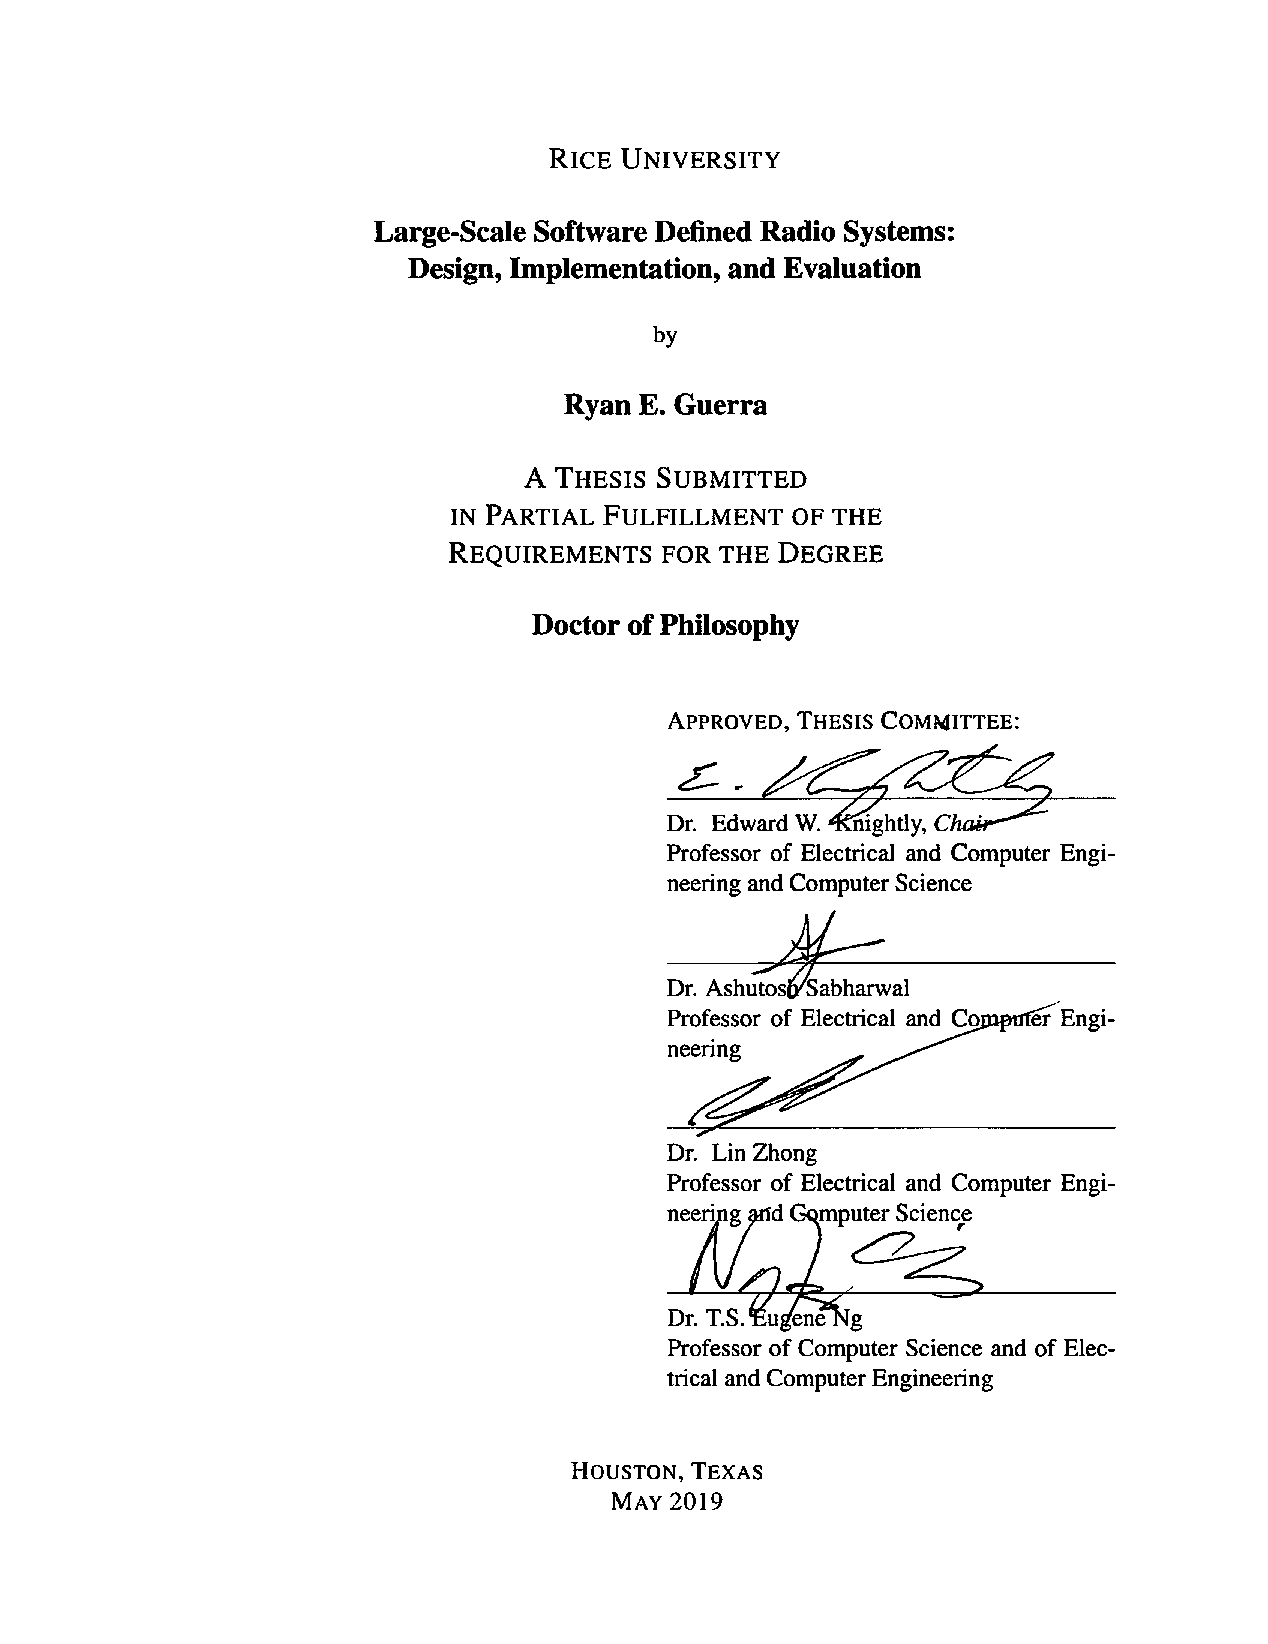
\includepdf[pages=-]{thesis_signature_page_signed.pdf}

% Include Abstract, Acknowledgement, and dedication if required.  It's in another file called "preface.tex"

\doublespacing
\thispagestyle{empty}
\begin{abstract}


	Since 2012, Television White Space (TVWS) systems have been permitted unlicensed operation on unused television channels between 50 to 800 MHz utilizing radio spectrum sharing techniques.

	Often considered ``beachfront property'' radio spectrum for their advantageous propagation characteristics, 6~MHz TVWS channels are nevertheless narrow relative to other unlicensed radio frequency bands and often fragmented, resulting in low network throughput and limiting their usefulness for modern, high-bandwidth applications.

	However, new many-antenna radio technologies have been shown to improve spectral efficiency beyond 100 bits/s/Hz, mitigating the need for wide channel bandwidths by leveraging spatial multiplexing.
	This presents an opportunity to deploy new unlicensed wireless networks that are large-scale in both range and speed as well as the number of coherent radios utilized for Multi-User Beamforming (MUBF).

	In this thesis, we design and implement the first scalable, agile, Software-Defined Radio (SDR) platform designed to support multi-user beamforming on TVWS.
	This design addresses key physical layer implementation barriers such as: fast automatic gain control, ultra-wideband power transfer networks, and distributed clocking architecture for scalable MUBF.

	Through an extensive series of indoor and outdoor measurements using our new platform, we show that in comparison to other unlicensed frequency bands, measured TVWS channels have temporal characteristics that are more beneficial for MUBF while maintaining nearly the same amount of spatial diversity.

	We leverage this new experimental insight to design an opportunistic MUBF protocol for 802.11af-like networks that can avoid all overhead associated with MUBF channel estimation by exploiting the high stability of fixed TVWS channels.
	We emulate this protocol based on empirical measurements and show that our opportunistic channel sounding protocol outperforms alternative 802.11af-based strategies for $4\times4$ or $8\times4$ MUBF when packets are short and modulation rates are high. 
	For high-order MUBF like $32\times16$, opportunistic channel sounding outperforms all alternatives by avoiding significant overhead that scales with the degree of spatial multiplexing.

	Through a comprehensive end-to-end system design addressing hardware, digital, and protocol challenges with final system validation, we develop a holistic new approach for leveraging TVWS to enable very large-scale, unlicensed wireless systems with gigabit network throughput.

\end{abstract}


%% COPY/PASTE ABSTRACT

%Since 2012, Television White Space (TVWS) systems have been permitted unlicensed operation on unused television channels between 50 to 800 MHz utilizing radio spectrum sharing techniques. Often considered "beachfront property" radio spectrum for their advantageous propagation characteristics, 6 MHz TVWS channels are nevertheless narrow relative to other unlicensed radio frequency bands and often fragmented, resulting in low network throughput and limiting their usefulness for modern, high-bandwidth applications.
%
%However, new many-antenna radio technologies have been shown to improve spectral efficiency beyond 100 bits/s/Hz, mitigating the need for wide channel bandwidths by leveraging spatial multiplexing. This presents an opportunity to deploy new unlicensed wireless networks that are large-scale in both range and speed as well as the number of coherent radios utilized for Multi-User Beamforming (MUBF).
%
%In this thesis, we design and implement the first scalable, agile, Software-Defined Radio (SDR) platform designed to support multi-user beamforming on TVWS. This design addresses key physical layer implementation barriers such as: fast automatic gain control, ultra-wideband power transfer networks, and distributed clocking architecture for scalable MUBF.
%
%Through an extensive series of indoor and outdoor measurements using our new platform, we show that in comparison to other unlicensed frequency bands, measured TVWS channels have temporal characteristics that are more beneficial for MUBF while maintaining nearly the same amount of spatial diversity.
%
%We leverage this new experimental insight to design an opportunistic MUBF protocol for 802.11af-like networks that can avoid all overhead associated with MUBF channel estimation by exploiting the high stability of fixed TVWS channels. We emulate this protocol based on empirical measurements and show that our opportunistic channel sounding protocol outperforms alternative 802.11af-based strategies for 4x4 or 8x4 MUBF when packets are short and modulation rates are high. For high-order MUBF like 32x16, opportunistic channel sounding outperforms all alternatives by avoiding significant overhead that scales with the degree of spatial multiplexing.
%
%Through a comprehensive end-to-end system design addressing hardware, digital, and protocol challenges with final system validation, we develop a holistic new approach for leveraging TVWS to enable very large-scale, unlicensed wireless systems with gigabit network throughput.



\begin{acknowledgements}

First and foremost I would like to thank my advisor, Dr. Edward Knightly, whose guidance, patience, and support has been invaluable in producing this thesis and providing me the space to be the best version of myself.  
Additionally, I would like to thank my thesis committee members for their comments, evaluation, and their time spent examining my work. 

I am grateful to my colleagues and especially my collaborators in the Rice ECE department without whom I would have learned very little.
Every Quixote needs their Sancho, and I am thrilled to have been able to tilt on my burro alongside some of the best researchers, dreamers, and friends you can find.
You know who you are and I owe you a drink and more.

I owe a large debt of gratitude to the previous generation of graduate students, particularly the WARP team: Patrick, Chris, Gareth, and Sid, for blazing a path that many of us have followed.
It may have been circuitous, but without it, we would still be lost in the woods.

How any family can put up with ten years of ambivalence is well beyond me, but I love you, Mom \& Dad.
You revealed the beautiful consistency of Science and then let me run double-blind to see what would happen. Well, I became an engineer, but not all is lost!

And finally, to the beautiful woman who beat me to the finish line only to run the race again while holding my hand: Rose, you continue to challenge and inspire me every day.

%The authors would like to thank the following people for their assistance in performing experiments included in this work: Rachel J. Gray (Rice University), Yuqiang Mu (Rice University), and Pablo Salvador (IMDEA Networks Institute). This research was supported by NSF grants CNS-1314822, CNS-1126478, CNS-1012831, and a grant from Cisco Systems, Inc.

\end{acknowledgements}

% Set the number of sectioning levels that get numbered and appear in the contents
\setcounter{secnumdepth}{3}
\setcounter{tocdepth}{2}
 
% I prefer half spacing for lists like this.
\onehalfspacing
\tableofcontents


%\printglossary[title={List of Symbols}]


\listoffigures
\listoftables

\chapter*{List of Acronyms}

\begin{acronym}
	\setlength{\parskip}{0ex}
	\setlength{\itemsep}{-3.5ex}

	\acro{WLAN}{Wireless LAN}
	\acro{TVWS}{Television-band White Space}
	%\acro{NLOS}{Non-Line-of-Sight}
	%\acro{LOS}{Line-of-Sight}
	\acro{MUBF}{Multi-User Beamforming}
	\acro{MIMO}{Multiple-Input, Multiple-Output}
	\acro{SISO}{Single-Input, Single-Output}
	\acro{MU-MIMO}{Multi-User MIMO}
	%\acro{MU-MIMO}{Multi-user Multiple-Input Multiple-Output}
	\acro{SDR}{Software-Defined Radio}
	\acro{ZFBF}{Zero-forcing Beamforming}
	\acro{TDMA}{Time-Division Multiple Access}
	\acro{CSI}{Channel State Information}
	\acro{OTA}{Over The Air}
	\acro{ISM}{Industrial, Scientific, and Medical}
	\acro{LNA}{Low-Noise Amplifier}
	\acro{FCC}{Federal Communications Commission}
	\acro{IC}{Integrated Circuit}
	\acro{CSIT}{Channel Side Information at the Transmitter}
	\acro{CSIR}{Channel Side Information at the Receiver}
	\acro{TDD}{Time-Division Duplex}
	\acro{FDD}{Frequency-Division Duplex}
	\acro{AGC}{Automatic Gain Control}
	\acro{ADC}{Analog-to-Digital Converter}
	\acro{DAC}{Digital-to-Analog Converter}
	\acro{UWB}{Ultra-WideBand}
	\acro{OFDM}{Orthogonal Frequency-Division Multiplexing}
	\acro{CFO}{Carrier Frequency Offset}
	\acro{STF}{802.11 Short Training Field}
	\acro{LTF}{802.11 Long Training Field}
	\acro{SNR}{Signal-to-Noise Ratio}
	\acro{MAC}{Media Access Control}
	\acro{PHY}{Physical}
	\acro{BER}{Bit Error Rate}
	\acro{EVM}{Error-Vector Magnitude}
	\acro{ASIC}{Application Specific Integrated Circuit}
	\acro{CSMA}{Carrier-Sense Multiple Access}
	\acro{SINR}{Signal-to-Interference-and-Noise Ratio}
	\acro{LS}{Least-Squares}
	\acro{MMSE}{Minimum Mean-Squared Error}
	\acro{MCS}{Modulation and Coding Scheme}
	%\acro{MUBF}{Multi-User Beam-Forming}
	\acro{SoC}{System-on-Chip}
	\acro{SBIR}{Small Business Innovation Grant}
	\acro{STTR}{Small Business Technology Transfer Grant}
	\acro{FPGA}{Field-Programmable Gate Array}
	\acro{FPRF}{Field-Programmable RF}
	\acro{CPU}{Central Processing Unit}
	\acro{WURC}{Wideband UHF Radio Card}
	\acro{NSF}{National Science Foundation}
	\acro{DSP}{Digital Signal Processor}
	%\acro{DPC}{Dirty Paper Coding}
	\acro{WISP}{Wireless Internet Service Provider}
	\acro{ISP}{Internet Service Provider}
	%\acro{DSL}{Digital Subscriber Line}
	\acro{adaptive}{Mobility-Aware Beamforming}
	\acro{spr}{Soft Pilot Reuse}
	\acro{IEEE}{Institute of Electrical and Electronics Engineers}
	\acro{3GPP}{3rd Generation Partnership Project}
	\acro{FARAD}{Frequency-Agile Radio}
	\acro{CAD}{Computer-Assisted Design}
	\acro{ETSI}{European Telecommunications Standards Institute}
	\acro{DSL}{Domain-Specific Language}
	\acro{SIR}{Signal-to-Interference Ratio}
	\acro{JT}{Joint Transmission}
	\acro{DPS}{Dynamic Point Selection}
	\acro{CBS}{Coordinated Beam-Switching}
	\acro{CS}{Coordinated Switching}

	% Included for FB proposal
	\acro{SRS}{Sounding Reference Signal}
	\acro{UpPTS}{Uplink Pilot Time Slots}
	\acro{SSF}{Special Sub-Frame}
	\acro{COTS}{Commercial Off-The-Shelf}
	\acro{UE}{LTE User Equipment}
	\acro{AoA}{Angle-of-Arrival}
	\acro{GPSDO}{GPS-Disciplined Oscillator}

	% Included for REG Thesis
	\acro{ACK}{Acknowledgement}
	\acro{LoS}{Line of Sight}
	\acro{NLoS}{Non-Line of Sight}
	\acro{BTS}{Base Station}
	\acro{CPE}{Consumer Premises Equipment}
	\acro{ROM}{Read-Only Memory}
	\acro{FSM}{Finite State Machine}
	\acro{LOFT}{Local Oscillator Feed-Through}
	\acro{FSPL}{Free-Space Path Loss}
	\acro{SINAD}{Signal-to-Noise-and-Distortion Ratio}
	\acro{RMS}{Root Mean Square}
	\acro{PPDU}{PLCP Protocol Data Unit}
	\acro{SPI}{Serial Programming Interface}
	\acro{RSSI}{Received Signal Strength Indicator}
	\acro{OOB}{Out-Of-Band}
	\acro{PCB}{Printed Circuit Board}
	\acro{SRF}{Self-Resonant Frequency}
	\acro{API}{Application Programming Interface}
	\acro{HDL}{Hardware Description Language}
	\acro{USB}{Universal Serial Bus}
	\acro{UART}{Universal Asynchronous Receiver/Transmitter}
	\acro{CoMP}{Coordinated Multi-Point}
	\acro{DDMTD}{Digital Dual Mixer Time Difference}
	\acro{CERN}{European Organization for Nuclear Research}
	\acro{PTP}{Precision Time Protocol}
	\acro{TIE}{Time Interval Error}
	\acro{CDR}{Clock Data Recovery}
	\acro{NI}{National Instruments}
	\acro{MEMS}{Micro-Electro-Mechanical Systems}
	\acro{GPS}{Global Positioning System}

	% Added for the 2016 ITC paper. REG 02/08/2016
	\acro{STA}{Station}
	\acro{AP}{Access Point}
	%\acro{CSIT}{Channel State Information at the Transmitter}
	\acro{GPIO}{General Purpose Input/Output}
	\acro{LAN}{Local Area Network}
	\acro{DPC}{Dirty Paper Coding}
	\acro{RSS}{Received Signal Strength}
	\acro{CBFR}{Compressed Beam-Forming Report}
	\acro{NDP}{Null Data Packet}
	\acro{ACK}{Acknowledgment}
	\acro{PLCP}{802.11 Physical Layer Convergence Procedure}
	\acro{MU-MIMO}{Multi-User MIMO}
	%\acro{SDR}{Software-Defined Radio}
	\acro{WARP}{Wireless open-Access Research Platform}
	\acro{CW}{Continuous Wave}
	\acro{DoF}{Degree of Freedom}
	\acro{FEC}{Forward Error Correction}
	\acro{FSR}{Full-Scale Range}
	\acro{ENOB}{Effective Number of Bits}
	\acro{PAPR}{Peak-to-Average Power Ratio}
	\acro{BSS}{Basic Service Set}
	\acro{DFS}{Dynamic Frequency Selection}
	\acro{DSSS}{Direct-Sequence Spread Spectrum}
	\acro{BPSK}{Binary Phase-Shift Keying}
	\acro{DCF}{Distributed Coordination Function}
	\acro{TPG}{Transducer Power Gain}
	\acro{EIRP}{Equivalent Isotropically Radiated Power}
	\acro{MAG}{Maximum Available Gain}
	\acro{PLL}{Phase Lock Loop}
	\acro{LVDS}{Low Voltage Differential Signaling}
	\acro{PDF}{Probability Distribution Function}
	\acro{SMT}{Surface-Mount Technology}
\end{acronym}


\bibliographystyle{IEEEtran}
\chapter*{List of Publications}

%\nobibliography*

\textbf{\textsc{Publications containing work that appears in part in this thesis.
}}
%\noindent\rule{8cm}{0.4pt}

\begin{itemize}
	\item R.~E. Guerra, N.~Anand, C.~W. Shepard, and E.~W. Knightly, ``{Opportunistic
  Channel Estimation for Implicit 802.11af MU-MIMO},'' in \emph{Proceedings of the 25th International Conference on Telecommunications},
  Wurzburg, Germany, Sept. 2016.
	\item C.~W. Shepard, R.~Doost-Mohammady, R.~E. Guerra, and L.~Zhong, ``{ArgosV3: An
  Efficient Many-Antenna Platform},'' in \emph{Proceedings of the 23rd Annual
  International Conference on Mobile Computing and Networking}.\hskip 1em plus
  0.5em minus 0.4em\relax ACM, 2017, pp. 501--503.
	\item C.~W. Shepard, J.~Ding, R.~E. Guerra, and L.~Zhong, ``{Understanding Real
  Many-Antenna MU-MIMO Channels},'' in \emph{Proceedings of IEEE Asilomar Signals,
  Systems, and Computers}, November 2016.
	\item N.~Anand, R.~E. Guerra, and E.~W. Knightly, ``{The Case for UHF-band
  MU-MIMO},'' \emph{Proceedings of ACM MobiCom}, September 2014.
	\item A.~Flores, R.~E. Guerra, E.~W. Knightly, P.~Ecclesine, and S.~Pandey, ``{IEEE
  802.11af: A Standard for TV White Space Spectrum Sharing},'' \emph{IEEE
  Communications Magazine}, October 2013.
	\item C.~Shepard, R.~Doost-Mohammady, J.~Ding, R.~E. Guerra, and L.~Zhong,
  ``Argosnet: A multi-cell many-antenna mu-mimo platform,'' November 2017.
	\item R.~E. Guerra, N.~Anand, and E.~Knightly, ``{Demo: An open-source development
  platform for long-range UHF-connected wifi hotspots},'' \emph{Proc. of ACM
  MobiCom}, September 2014.
	\item R.~E. Guerra, N.~Anand, and E.~W. Knightly, ``{Demo: A Platform for At-Scale
  Wideband UHF MU-MIMO Systems},'' \emph{Proc. of USENIX NSDI}, April 2014.
\end{itemize}


\textbf{\textsc{3rd-party publications utilizing the \ac{WURC} \ac{SDR} platform.}}

%\noindent\rule{8cm}{0.4pt}

\begin{itemize}
	\item T.~Wei, S.~Wang, A.~Zhou, and X.~Zhang, ``Acoustic eavesdropping through
  wireless vibrometry,'' in \emph{Proceedings of the 21st Annual International
  Conference on Mobile Computing and Networking}.\hskip 1em plus 0.5em minus
  0.4em\relax ACM, 2015, pp. 130--141.
	\item S.~Sur and X.~Zhang, ``Bridging link power asymmetry in mobile whitespace
  networks,'' in \emph{Computer Communications (INFOCOM), 2015 IEEE Conference
  on}.\hskip 1em plus 0.5em minus 0.4em\relax IEEE, 2015, pp. 1176--1184.
	\item X.~Zhang and E.~W. Knightly, ``Watch: Wifi in active tv channels,'' \emph{IEEE
  Transactions on Cognitive Communications and Networking}, vol.~2, no.~4, pp.
  330--342, 2016.
	\item C.~A. Tarver, ``Sub-band digital predistortion for noncontiguous carriers:
  Implementation and testing,'' Ph.D. dissertation, Rice University, 2016,
  {Masters Thesis}.
	\item X.~Zhang, ``Watch: Enabling wifi in active tv channels,'' Ph.D. dissertation,
  Rice University, 2014, {Masters Thesis}.
\end{itemize}



%%%%%%%%%%% ACRO DEFS %%%%%%%%%%%%
%\printglossary[type=acronym, title={List of Acronyms}] %={List of Acronyms}]
%
\begin{acronym}
	\setlength{\parskip}{0ex}
	\setlength{\itemsep}{-3.5ex}

	\acro{WLAN}{Wireless LAN}
	\acro{TVWS}{Television-band White Space}
	%\acro{NLOS}{Non-Line-of-Sight}
	%\acro{LOS}{Line-of-Sight}
	\acro{MUBF}{Multi-User Beamforming}
	\acro{MIMO}{Multiple-Input, Multiple-Output}
	\acro{SISO}{Single-Input, Single-Output}
	\acro{MU-MIMO}{Multi-User MIMO}
	%\acro{MU-MIMO}{Multi-user Multiple-Input Multiple-Output}
	\acro{SDR}{Software-Defined Radio}
	\acro{ZFBF}{Zero-forcing Beamforming}
	\acro{TDMA}{Time-Division Multiple Access}
	\acro{CSI}{Channel State Information}
	\acro{OTA}{Over The Air}
	\acro{ISM}{Industrial, Scientific, and Medical}
	\acro{LNA}{Low-Noise Amplifier}
	\acro{FCC}{Federal Communications Commission}
	\acro{IC}{Integrated Circuit}
	\acro{CSIT}{Channel Side Information at the Transmitter}
	\acro{CSIR}{Channel Side Information at the Receiver}
	\acro{TDD}{Time-Division Duplex}
	\acro{FDD}{Frequency-Division Duplex}
	\acro{AGC}{Automatic Gain Control}
	\acro{ADC}{Analog-to-Digital Converter}
	\acro{DAC}{Digital-to-Analog Converter}
	\acro{UWB}{Ultra-WideBand}
	\acro{OFDM}{Orthogonal Frequency-Division Multiplexing}
	\acro{CFO}{Carrier Frequency Offset}
	\acro{STF}{802.11 Short Training Field}
	\acro{LTF}{802.11 Long Training Field}
	\acro{SNR}{Signal-to-Noise Ratio}
	\acro{MAC}{Media Access Control}
	\acro{PHY}{Physical}
	\acro{BER}{Bit Error Rate}
	\acro{EVM}{Error-Vector Magnitude}
	\acro{ASIC}{Application Specific Integrated Circuit}
	\acro{CSMA}{Carrier-Sense Multiple Access}
	\acro{SINR}{Signal-to-Interference-and-Noise Ratio}
	\acro{LS}{Least-Squares}
	\acro{MMSE}{Minimum Mean-Squared Error}
	\acro{MCS}{Modulation and Coding Scheme}
	%\acro{MUBF}{Multi-User Beam-Forming}
	\acro{SoC}{System-on-Chip}
	\acro{SBIR}{Small Business Innovation Grant}
	\acro{STTR}{Small Business Technology Transfer Grant}
	\acro{FPGA}{Field-Programmable Gate Array}
	\acro{FPRF}{Field-Programmable RF}
	\acro{CPU}{Central Processing Unit}
	\acro{WURC}{Wideband UHF Radio Card}
	\acro{NSF}{National Science Foundation}
	\acro{DSP}{Digital Signal Processor}
	%\acro{DPC}{Dirty Paper Coding}
	\acro{WISP}{Wireless Internet Service Provider}
	\acro{ISP}{Internet Service Provider}
	%\acro{DSL}{Digital Subscriber Line}
	\acro{adaptive}{Mobility-Aware Beamforming}
	\acro{spr}{Soft Pilot Reuse}
	\acro{IEEE}{Institute of Electrical and Electronics Engineers}
	\acro{3GPP}{3rd Generation Partnership Project}
	\acro{FARAD}{Frequency-Agile Radio}
	\acro{CAD}{Computer-Assisted Design}
	\acro{ETSI}{European Telecommunications Standards Institute}
	\acro{DSL}{Domain-Specific Language}
	\acro{SIR}{Signal-to-Interference Ratio}
	\acro{JT}{Joint Transmission}
	\acro{DPS}{Dynamic Point Selection}
	\acro{CBS}{Coordinated Beam-Switching}
	\acro{CS}{Coordinated Switching}

	% Included for FB proposal
	\acro{SRS}{Sounding Reference Signal}
	\acro{UpPTS}{Uplink Pilot Time Slots}
	\acro{SSF}{Special Sub-Frame}
	\acro{COTS}{Commercial Off-The-Shelf}
	\acro{UE}{LTE User Equipment}
	\acro{AoA}{Angle-of-Arrival}
	\acro{GPSDO}{GPS-Disciplined Oscillator}

	% Included for REG Thesis
	\acro{ACK}{Acknowledgement}
	\acro{LoS}{Line of Sight}
	\acro{NLoS}{Non-Line of Sight}
	\acro{BTS}{Base Station}
	\acro{CPE}{Consumer Premises Equipment}
	\acro{ROM}{Read-Only Memory}
	\acro{FSM}{Finite State Machine}
	\acro{LOFT}{Local Oscillator Feed-Through}
	\acro{FSPL}{Free-Space Path Loss}
	\acro{SINAD}{Signal-to-Noise-and-Distortion Ratio}
	\acro{RMS}{Root Mean Square}
	\acro{PPDU}{PLCP Protocol Data Unit}
	\acro{SPI}{Serial Programming Interface}
	\acro{RSSI}{Received Signal Strength Indicator}
	\acro{OOB}{Out-Of-Band}
	\acro{PCB}{Printed Circuit Board}
	\acro{SRF}{Self-Resonant Frequency}
	\acro{API}{Application Programming Interface}
	\acro{HDL}{Hardware Description Language}
	\acro{USB}{Universal Serial Bus}
	\acro{UART}{Universal Asynchronous Receiver/Transmitter}
	\acro{CoMP}{Coordinated Multi-Point}
	\acro{DDMTD}{Digital Dual Mixer Time Difference}
	\acro{CERN}{European Organization for Nuclear Research}
	\acro{PTP}{Precision Time Protocol}
	\acro{TIE}{Time Interval Error}
	\acro{CDR}{Clock Data Recovery}
	\acro{NI}{National Instruments}
	\acro{MEMS}{Micro-Electro-Mechanical Systems}
	\acro{GPS}{Global Positioning System}

	% Added for the 2016 ITC paper. REG 02/08/2016
	\acro{STA}{Station}
	\acro{AP}{Access Point}
	%\acro{CSIT}{Channel State Information at the Transmitter}
	\acro{GPIO}{General Purpose Input/Output}
	\acro{LAN}{Local Area Network}
	\acro{DPC}{Dirty Paper Coding}
	\acro{RSS}{Received Signal Strength}
	\acro{CBFR}{Compressed Beam-Forming Report}
	\acro{NDP}{Null Data Packet}
	\acro{ACK}{Acknowledgment}
	\acro{PLCP}{802.11 Physical Layer Convergence Procedure}
	\acro{MU-MIMO}{Multi-User MIMO}
	%\acro{SDR}{Software-Defined Radio}
	\acro{WARP}{Wireless open-Access Research Platform}
	\acro{CW}{Continuous Wave}
	\acro{DoF}{Degree of Freedom}
	\acro{FEC}{Forward Error Correction}
	\acro{FSR}{Full-Scale Range}
	\acro{ENOB}{Effective Number of Bits}
	\acro{PAPR}{Peak-to-Average Power Ratio}
	\acro{BSS}{Basic Service Set}
	\acro{DFS}{Dynamic Frequency Selection}
	\acro{DSSS}{Direct-Sequence Spread Spectrum}
	\acro{BPSK}{Binary Phase-Shift Keying}
	\acro{DCF}{Distributed Coordination Function}
	\acro{TPG}{Transducer Power Gain}
	\acro{EIRP}{Equivalent Isotropically Radiated Power}
	\acro{MAG}{Maximum Available Gain}
	\acro{PLL}{Phase Lock Loop}
	\acro{LVDS}{Low Voltage Differential Signaling}
	\acro{PDF}{Probability Distribution Function}
	\acro{SMT}{Surface-Mount Technology}
\end{acronym}

%%%%%%%%%%%%%%%%%%%%%%%%%%%%%%%%%%%

%\chapter*{List of Notation}
%\printglossary[title=Notation]
%%%%%%%%%%%%%%%%%%%%%%%%%%%%%%%%%%


% End roman numerals, begin numbering in Arabic starting with the text
\end{romanpages}
 
\doublespacing

\acresetall

% https://tex.stackexchange.com/questions/76273/multiple-pdfs-with-page-group-included-in-a-single-page-warning
\pdfsuppresswarningpagegroup=1

%###########################################################
\chapter{Introduction}
\section{Thesis Motivation}
\label{sec_introduction}

IEEE 802.11, or ``Wi-Fi'' is one of the most successful technologies in the world.
	As of today, the global installed base of 802.11-powered wireless devices has grown past 9.5~billion units, with over 3~billion wireless sensors, phones, computers, and other connected devices shipping each year\cite{wifi2018installed}.
	This large and vibrant device ecosystem was enabled by the establishment of the unlicensed \ac{ISM} wireless bands in 1985, unleashing decades of rapid wireless technology innovation.
	
	We saw a similar dynamic playing out when in 2012 the switch to digital broadcast television from analog broadcasts released hundreds of megahertz of valuable radio spectrum in the VHF and UHF frequency bands for 802.11-like unlicensed purposes \cite{fcc2010second, fcc2012third, fcc2015ro}.
	Known for their excellent propagation characteristics \cite{flores2013ieee80211af, stone1997nist}, these \acf{TVWS} frequencies between 54~MHz to 608~MHz in the United States and 470~MHz to 790~MHz in Europe may now be used by \emph{unlicensed} secondary devices in the many locations where primary television broadcasters are not operating.

	However, there are significant implementation challenges for \ac{TVWS} networks and devices if they are to meet the performance and user experience targets of today's multi-gigabit 802.11 systems.
	Practical \ac{TVWS} channel availability is limited in many locations and in most cases the available channels are non-contiguous.
	Without the ability to practically bond the dozens of 6~MHz \ac{TVWS} channels that would be needed to match the performance of wide 80+80~MHz channels in 802.11ac/ax \ac{ISM} bands, it instead becomes necessary to focus on utilizing the available radio spectrum with high spectral efficiency.

	In this, we are in luck; advancements in radio technology now allow us to create highly flexible and agile \acf{SDR} systems that adapt center frequency and waveform easily to match the local RF landscape and regulatory limitations.
	Cognitive radio technologies allow systems to dynamically detect and share scarce radio resources with other systems for optimal radio spectrum utilization.
	In addition, the computational and system complexity of large-scale \ac{MU-MIMO} beamforming can now be addressed with modern radio design and computational platforms, allowing us to increase the capacity of wireless systems along the complementary axis of spatial multiplexing, rather than just increasing channel bandwidth.
	
	As we demonstrate, serious system limitations exist both in hardware design and protocol design that limit the amount of spatial diversity that \ac{TVWS} radio systems can practically leverage.		
	Therefore, we seek to design new \ac{TVWS} radio systems that can realize the promise of new ``low-band'' unlicensed radio spectrum and bring the \ac{TVWS} opportunity to fruition.
	
			\ac{TVWS} systems represent an opportunity to provide 802.11-like connectivity on an unprecedented scale, reaching new environments and applications that can not be efficiently served with standard 802.11ac/ax.
			For the purposes of this thesis, we consider ``large-scale'' to have two meanings: first, we wish to design wireless systems that can provide high-speed connectivity on the campus or city-scale distances typically associated with television broadcasters but out of reach for other 802.11 systems; second, we wish to design systems that highly leverage spatial multiplexing, scaling the number of spatial streams beyond the $4\times 4$ or $8\times 8$ numbers seen in 802.11ac/ax standards, in order to increase the throughput performance of 802.11af \ac{TVWS} system on part with other 802.11 standards.

\section{Thesis Contributions}
\label{sec_contributions}

In this thesis, we develop the tools and understanding necessary to design, implement, and evaluate large-scale and high-speed wireless networks utilizing \ac{TVWS} radio spectrum.

	We start in Chapter~\ref{sec_background_chapter} with a discussion of necessary background information useful as context, as well as an introduction to the notation used throughout this thesis.

	Chapter~\ref{sec_wurc} presents the design, implementation, and testing of a flexible software-defined radio platform that implements 802.11af and \ac{MU-MIMO} beamforming in a custom hardware platform that we design and manufacture.
	In order to realize this new platform, we develop solutions to multiple physical layer challenges:
\begin{itemize}
	\item We design and test several iterations of \ac{WURC}, a new agile \ac{SDR} platform with an operational frequency range of 50 - 3800~MHz, and integrate it with WARPv3 to create the most agile MU-MIMO SDR platform at the time with range from 50 - 5800~MHz,
	%\item We develop analog calibration algorithms suited for tuning agile \acp{SDR} with wide operational bandwidths, 
	\item We design and test power transfer impedance matching circuits for \ac{TVWS} with over 40\% bandwidth using numerical circuit synthesis and optimization techniques,
	\item We design a generic fast automatic gain control for \acp{SDR} that avoids utilizing external power estimation components and still meets strict 802.11 timing constraints,
	\item We design an extensive library of software drivers and logic blocks that enable both real-time 802.11ac/af-like communication on our \ac{SDR} platform as well as the ability to scale operation to 8x8 802.11ac/af-like MU-MIMO,
	\item We design, implement, and test several methods for reference clock sharing between remote coherent radios heads in a live hardware system for scalable many-antenna \ac{MIMO}.
\end{itemize}
	When taken together, our system design contributions constitute the development of the world's first open-source software-defined \ac{MU-MIMO} \ac{TVWS} testbed.
	We have made the design files for all \ac{WURC} \acp{PCB} available open-source \cite{guerra2012wurc_pcb}.
	
	In Chapter~\ref{sec_env_study_chapter}, we leverage our new \ac{MU-MIMO} platform to perform a comprehensive series of environmental measurement studies of indoor and outdoor \ac{MU-MIMO} channels in various static and mobile scenarios in unlicensed and \ac{ISM} bands from 470 - 5800~MHz.
	We first start with an early study of a prototype \ac{SISO} \ac{TVWS} network that we installed in a Houston neighborhood.
	As the first residential \ac{TVWS} network deployed, we are able to confirm the superior propagation performance of 802.11af systems while exposing serious platform and system-level limitations.
	
	We then proceed to utilize our newly developed \ac{TVWS} \ac{SDR} system from Chapter~\ref{sec_wurc} and perform the first study of \ac{MU-MIMO} \ac{TVWS} channel dynamics, finding that spatial diversity is preserved in \ac{TVWS} channels while system temporal dynamics are much improved compared to higher-frequency \ac{ISM} bands.

	In Chapter~\ref{sec_protocols_chapter}, we present the design and analysis of an opportunistic channel sounding protocol for 802.11af-like systems that increases spectral efficiency by two orders of magnitude over \ac{SISO} systems.
	For this design, we leverage the advantageous temporal dynamics of \ac{TVWS} observed in our measurement studies in order to opportunistically estimate \ac{CSI} information using implicit feedback from control and data packets already on the air.
	This design allows \ac{TVWS} multi-user beamforming systems to scale the number of simultaneous data streams while mitigating the channel sounding overhead incurred by the 802.11af protocol when estimating channel state information.
	
	Chapter~\ref{sec_related_chapter} reviews and compares the current literature in related fields, providing additional context for those readers wishing to learn more.
	
	Finally, Chapter~\ref{sec_conclusion_chapter} concludes this thesis with a discussion of our findings and some future directions to take \ac{TVWS} and \ac{MU-MIMO} systems.


%###########################################################

\chapter{Background}
\label{sec_background_chapter}
\section{Introduction}
\label{sec:background}

%In this chapter we provide background for the 802.11 wireless communications standard, including its 802.11af \ac{TVWS} extensions, with a focus on \ac{MU-MIMO} transmission techniques in 802.11ac/ax and key performance factors for general \ac{MU-MIMO}.
In this chapter we provide background for wireless communications systems with a focus on \ac{MU-MIMO} transmission techniques such as those used in \ac{IEEE} 802.11ac/ax and key performance factors for \ac{MU-MIMO}.

We will also review software-defined radios and their implementation in order to provide context for the innovative \ac{SDR} system design in this thesis.


	%#######################################################
	%\section{Wi-Fi: the IEEE 802.11 Standard}
	%\label{sec:back_80211}
%
%\iftoggle{isready} {
%
	%As the second widespread use of spectrum sharing,\footnote{The IEEE 802.11a standard includes \ac{DFS} sensing and protection of radar signals between [5.260, 5.700]~GHz.} 
%
	%\rgnote{Basic background about 802.11, random access, frame structure, terminology. 802.11ac extension for MU-MIMO. This is where \ac{STA} and \ac{AP} get defined}
%
	%%#######################################################
	%\subsection{IEEE 802.11af Standard Extension for TVWS}
	%\label{sec:back_80211af}
%
	%\rgnote{Motivation and constraints of 802.11af, pulling from my IEEE article content. Database vs. sensing approaches--we focus on database-driven approaches.}
%
	%Wifi over TVWS: \cite{bahl2009white}
%
%}{ \rgnote{The WiFi background section is pending.}}

%#######################################################
\section{Multi-user Beamforming}
\label{sec_mubf_back}
	Multi-user beamforming is a multi-antenna transmission technique that allows a transmitter to spatially reuse a wireless channel by transmitting multiple concurrent data streams on the same radio frequency using linear pre-coding.
	This is achieved in two steps: first, the wireless channel is estimated and represented as a complex matrix $\mathbf{H}_c\in \mathbb{C}^{M\times K}$ representing the narrowband scalar channel weights for each path between $M$ transmit antennas and $K$ receive antennas for each of $C$ narrowband subcarriers within the wideband.
	Shown in Figure~\ref{fig_h_matrix}, this wireless channel representation is called the \ac{OFDM} wideband channel representation since it treats each subcarrier independently and is used for \ac{OFDM} transmission techniques \cite{perahia2008}.
	An underlying assumption for this channel model is that the bandwidth of the subcarriers is chosen such that a complex scalar coefficient, $h_{mkc}$, is sufficient to accurately represent the magnitude and phase of the channel state of subcarrier $c$.
	For the remainder of this thesis, we will forgo the subscript $c$ when discussing the wireless $\mathbf{H}$ matrix channel representation.
	
	\begin{figure}[h]
\centering
  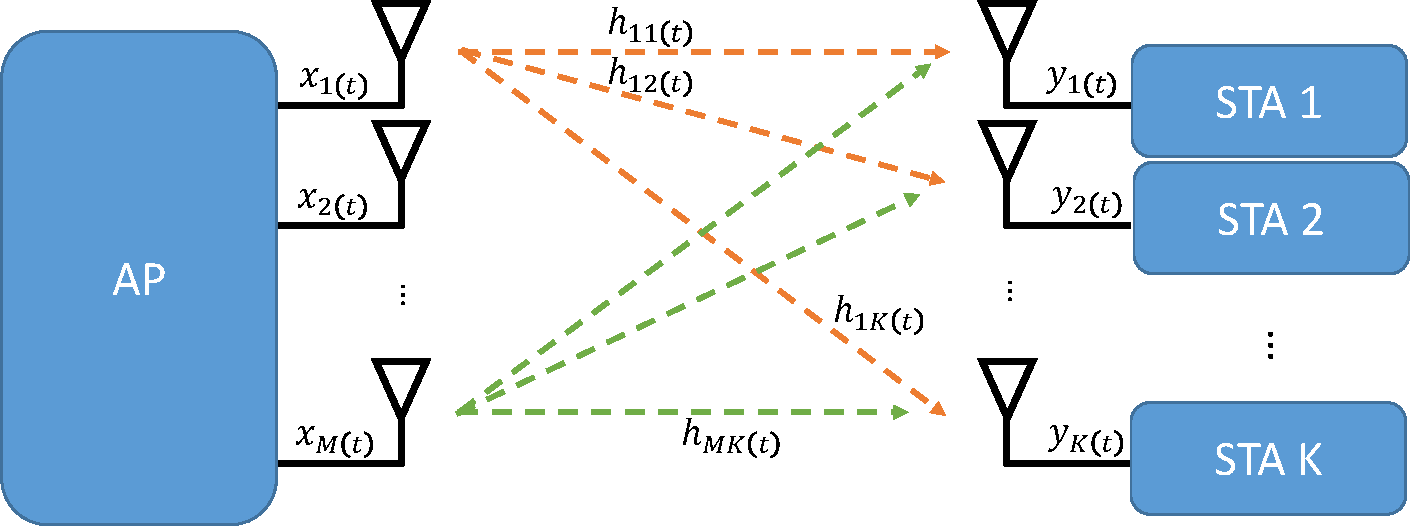
\includegraphics[width=4.5in]{figs/general/beamforming_h_matrix}   
    \caption{H-matrix representation of the physical wireless channel.}
\label{fig_h_matrix}
\end{figure}

	The second step for multi-user beamforming is the application of downlink beam-steering weights.
	Each data stream for each of $K$ receive antennas, $\mathbf{S}\in \mathbb{C}^{K\times 1}$, is left-multiplied by a matrix of complex steering weights $\mathbf{W}\in \mathbb{C}^{M\times K}$  resulting in $\mathbf{X} = \mathbf{W}\cdot \mathbf{S} \in\mathbb{C}^{1\times M}$ pre-coded signals containing a linear combination of each data stream to transmit from each of the \ac{AP}'s $M$ antennas.
	
	The $K$ antennas may each be on a single separate \ac{STA} or may be in any combination where a subset of $K$ is on a single receiver \ac{STA}.
	When all $K$ are on a single \ac{STA} this reduces to a simple single-user \ac{MIMO} transmission.
	The key distinction is that \acp{STA} are independent receivers in \ac{MU-MIMO} transmissions and do not share receive information between each other.


%#######################################################
\subsection{Pre-coding Weight Selection}
	The linear pre-coding weights $\textbf{W}$, also called ``beam-steering weights,'' are chosen such that the interference between the parallel streams is minimal.  
	To compute these weights, the transmitter must first measure the channel state matrix $\textbf{H}$.
	The optimal method of constructing the steering matrix is \acf{DPC} \cite{costa1983dpc}; however, its computational complexity makes it impractical to implement in full. 
	
	
	Instead, a practical method for calculating $\mathbf{W}$ from $\mathbf{H}$ that approaches optimal performance is \ac{ZFBF}\cite{goldsmith2006zf}.  
 Zero-forcing drives interference between spatial streams to zero, and can be inefficient when users' \ac{CSI} is not sufficiently orthogonal \cite{aryafar2010design} or in low \ac{SNR} environments.
 \ac{ZFBF} requires calculation of the $\mathbf{H}$ matrix's Moore-Penrose pseudo-inverse:
\begin{equation}
\mathbf{W} = \mathbf{H}^\dagger =  (\mathbf{H}^\textsc{H} \mathbf{H})^{-1} \mathbf{H}^\textsc{H}, \label{eq:zf}
\end{equation}
where $(\cdot)^\textsc{H}$ represents the matrix conjugate transpose and $(\cdot)^\dagger$ is the Moore-Penrose pseudo-inverse.
%When the transmitter precodes with perfect \ac{ZFBF} weights, $\mathbf{W}$, signals ideally cancel the effects of the wireless channel at the receiver, allowing each user to receive their own, independent streams.

	A key element of \ac{ZFBF} is the zero-interference condition which is a direct result of the pseudo-inverse.
	Because $\textbf{W}=\textbf{H}^\dagger$, then $\textbf{H}\cdot\textbf{W}$ is the identity matrix, meaning that the interference from the data stream from user $k=i$ on the data stream for user $k=j$ is nulled and vice versa.
	\ac{ZFBF} pre-codes the transmitted data streams such that the combined wireless channel between the transmitter and the receivers is separated.
	If \ac{ZFBF} works perfectly, we can express the pre-coded transmission $\mathbf{X}$ as:
\begin{align}
\mathbf{X} = \mathbf{W} \cdot \mathbf{S} \xrightarrow[\mathbf{H}]{\text{Transmit}} & \mathbf{H}\cdot (\mathbf{W} \cdot \mathbf{S}) \notag \\
 = & \cancel{\mathbf{H}} \cdot (\cancel{\mathbf{W}} \cdot \mathbf{S}) = \mathbf{S}
\end{align}

	There are additional ways to calculate the pre-coding weights for digital beamforming systems; two of the most notable alternatives are conjugate beamforming \cite{yang2013performance} and \ac{MMSE} beamforming \cite{joham2005linear}, both of which are optimal under certain conditions.
	In our work, due to the computational complexity of \ac{MMSE} beamforming implementation, we focus on the zero-forcing beamforming technique for \ac{MU-MIMO}, though most of the insights and systems could be easily applied to alternative types of beamforming.


%#######################################################
\subsection{MIMO Channel Correlation and Temporal Correlation Function}
%\rgnote{Beamforming Performance Limits Clean this notation and discusion up}
	The key to the success of the precoding operation is that $\textbf{H}\cdot \textbf{W}$ is designed to reduce to the identity matrix so the transmitted streams are received separately at each receiver.
	We are generally interested in two characteristics of $\textbf{H}$ that can degrade the performance of this precoding operation: an ill-conditioned $\textbf{H}$ \cite{zhong2011distribution} or an out-dated $\textbf{H}$ \cite{kaltenberger2008correlation}, each related to different statistical correlation concepts.

\textbf{MIMO Channel Correlation.}
	An ill-conditioned $\textbf{H}$ matrix renders matrix inversion inaccurate \cite{greenbaum2012numerical, peel2005vector} which is required to calculate the pseudo-inverse in Equation~\ref{eq:zf}.
	This results in $\textbf{H}\cdot \textbf{W}$ becoming far less likely to equal $\textbf{I}$ and causes ``inter-stream interference'' as a result of beamformed data streams interfering and degrading the received signal strength of a data stream to its intended receiver \cite{kaltenberger2008correlation}.
	Ill-conditioned $\textbf{H}$ matrices can be a result of \ac{MIMO} channel correlation, a characteristic of the physical arrangement of the \ac{MIMO} antenna array or the wireless environment that measures how similar the independent paths between \ac{MIMO} antennas are to each other by relating their individual path random processes \cite{loyka2001channel}.
	With sufficiently high \ac{MIMO} channel correlation, any particular realization of the matrix channel random process is likely to not be full-rank, which makes it non-invertible or singular \cite{peel2005vector}.
	Increasing channel correlation in general results in a decrease in \ac{SNR} for a \ac{MIMO} system \cite{loyka2001channel}, and can be interpreted as a lack of physically independent information channels in the environment or radio array available to convey information.

\textbf{Channel Correlation Function.}
	Channel correlation is a property of the wireless \ac{MIMO} channel matrix $\textbf{H}$ and is not to be confused with the channel \emph{temporal correlation} function, which is a property of the individual channel random process $h_{mk}$ and indicates how correlated the channel condition is as a function of time.
	Temporal correlation is the expected autocorrelation between channel snapshots at varying intervals of time calculated as described in \cite{wallace2003experimental}.
	An intrinsic property of the channel random process, an empirical temporal correlation function can be estimated from time series of channel state observations.
	The empirical correlation coefficient for a single channel $\rho$ at time interval $\ell$ is defined as:
\begin{align}
\rho_\ell = \frac{\mathbb{E}\big[h_{m}[k]h^{*}_{mn}[k+\ell]\big]}{\mathbb{E}\big[h_{mn}[k]h^{*}_{mn}[k]\big]}
\label{eq_corr_coeff}
\end{align}
where the expectation is calculated for all combinations of transmit antenna $m$, receive antenna $n$ and starting time sample $k$.
 %Assuming each channel path is generated by the same random process, the resulting empirical correlation functions for each \ac{MIMO} channel path can be averaged together for an overall estimate of channel temporal performance.

	Out-dated $\textbf{H}$ matrices are a direct result of the latency between the measurement of the $\textbf{H}$ matrix and the transmission of the $\textbf{W}$ precoded data streams.  
	Increased time between the measurement of $\textbf{H}$ and the transmission of $\textbf{W}\cdot \textbf{S}$, results in a higher probability of incorrect transmit precoding.  
	Essentially, the transmitter measures $\textbf{H}_{t}$ and then calculates $\textbf{W}_t = \textbf{H}_t^\dagger$.
However, the subsequent precoded transmission is $\textbf{H}_{t+\Delta}\cdot \textbf{W}_{t}$, which may not equal $\textbf{I}$ since the channel has changed since estimation at time $t$.
	The temporal correlation function is a way of estimating how much the channel will change over time.
	Whether or not $\textbf{H}_{t}=\textbf{H}_{t+\Delta}$ is based on environmental variability and user mobility; and, like channel conditioning, is also an environment and frequency dependent characteristic. 

	While a large number of studies have characterized the indoor and outdoor propagation environment for the purpose of network planning and algorithm design, few are applicable to evaluating \ac{MU-MIMO} performance and most have focused on a single frequency band \cite{boyer2007mimo, hammons2008cooperative, jung2011multipath}.
	This makes measurement studies of different frequencies and radio technologies difficult to compare.

At the same time, the implementation complexity and computation required for real-time implementation of multi-carrier \ac{MU-MIMO} has traditionally been prohibitive for software-defined radio platforms \cite{aryafar2010design}, thus providing a challenge to empirical measurement of \ac{MU-MIMO} performance.

%\subsection{Systemic CSI Estimation Error}
%\label{sec_systemic_csi_error}
%
%\rgnote{review this section--I wanted to include it because I constantly have to explain this and it's not immediately clear until you actually prove it with math. This might get cut.}
%
%Recall that given a channel estimate, $\Hb$, the precoding weights for the zero-forcing transmitter are $\mathbf{W} = \mathbf{H}^\dagger =  (\mathbf{H}^\textsc{H} \mathbf{H})^{-1} \mathbf{H}^\textsc{H}$.
	%Arbitrary magnitude and phase offsets may be present in any one estimate of the \ac{CSI} due to receive gain control or timing estimation jitter, respectively.
	%These are normal effects in \ac{OFDM} transceivers that are compensated by the receive \ac{OFDM} channel equalization, yet become part of the channel estimation at the receiver \cite{park2003timing, breit2009coherencetime}.
	%While not a new finding, it is useful to discuss the effect that these types of systemic \ac{CSI} estimation error components and how they differ from estimation error due to stale \ac{CSI}.
	%
	%We define a systemic \ac{CSI} estimation error as any error matrix $\Phi \in \mathbb{C}^{M\times K}$ that can be represented as a diagonal matrix: $\Phi = diag(\alpha_1,\ldots,\alpha_M)$.
%
	%It is a well-known property of beamforming that the input \ac{CSI}, $\Hb$, can be perturbed by an arbitrary diagonal matrix $\Phi = diag(\alpha_1,\ldots,\alpha_M)$ such that the \ac{CSI} used for precoding is $\hat{\Hb} = \Hb\Phi$.
	%The resulting original beamformed streams, $\mathbf{Y} = \mathbf{W}\Hb$, and the received perturbed beamformed streams, $\mathbf{Y'} = \hat{\Hb}^\dagger\Hb$, still preserve the orthogonal separation of the user streams owing to the diagonality of $\Phi$.
	%In other words, $\mathbf{Y'} = (\Phi)^{-1}\mathbf{Y}$, and beamforming performance is not significantly impacted by such measurement artifacts.
%
	%This is a powerful result \rgnote{finish this section when I'm less tired}

%#######################################################
%\section{Many-Antenna and Massive MIMO}
%\label{sec_mami_back}
%
%\iftoggle{isready} {
%
%
%}{ \rgnote{The Massive MIMO background section is pending.}}

%#######################################################
\section{Software Defined Radio Architecture}
\label{sec_sdr_back}

A \acf{SDR} is a radio that replaces analog signal processing components with programmable digital logic.
This radio architecture increases flexibility by replacing analog signal processing components with digital logic, enabling the use of more flexible and complex waveforms such as \ac{OFDM} and simplifying cross-layer system design.

\begin{figure}[ht] % Idealized AGC block diagram
\centering
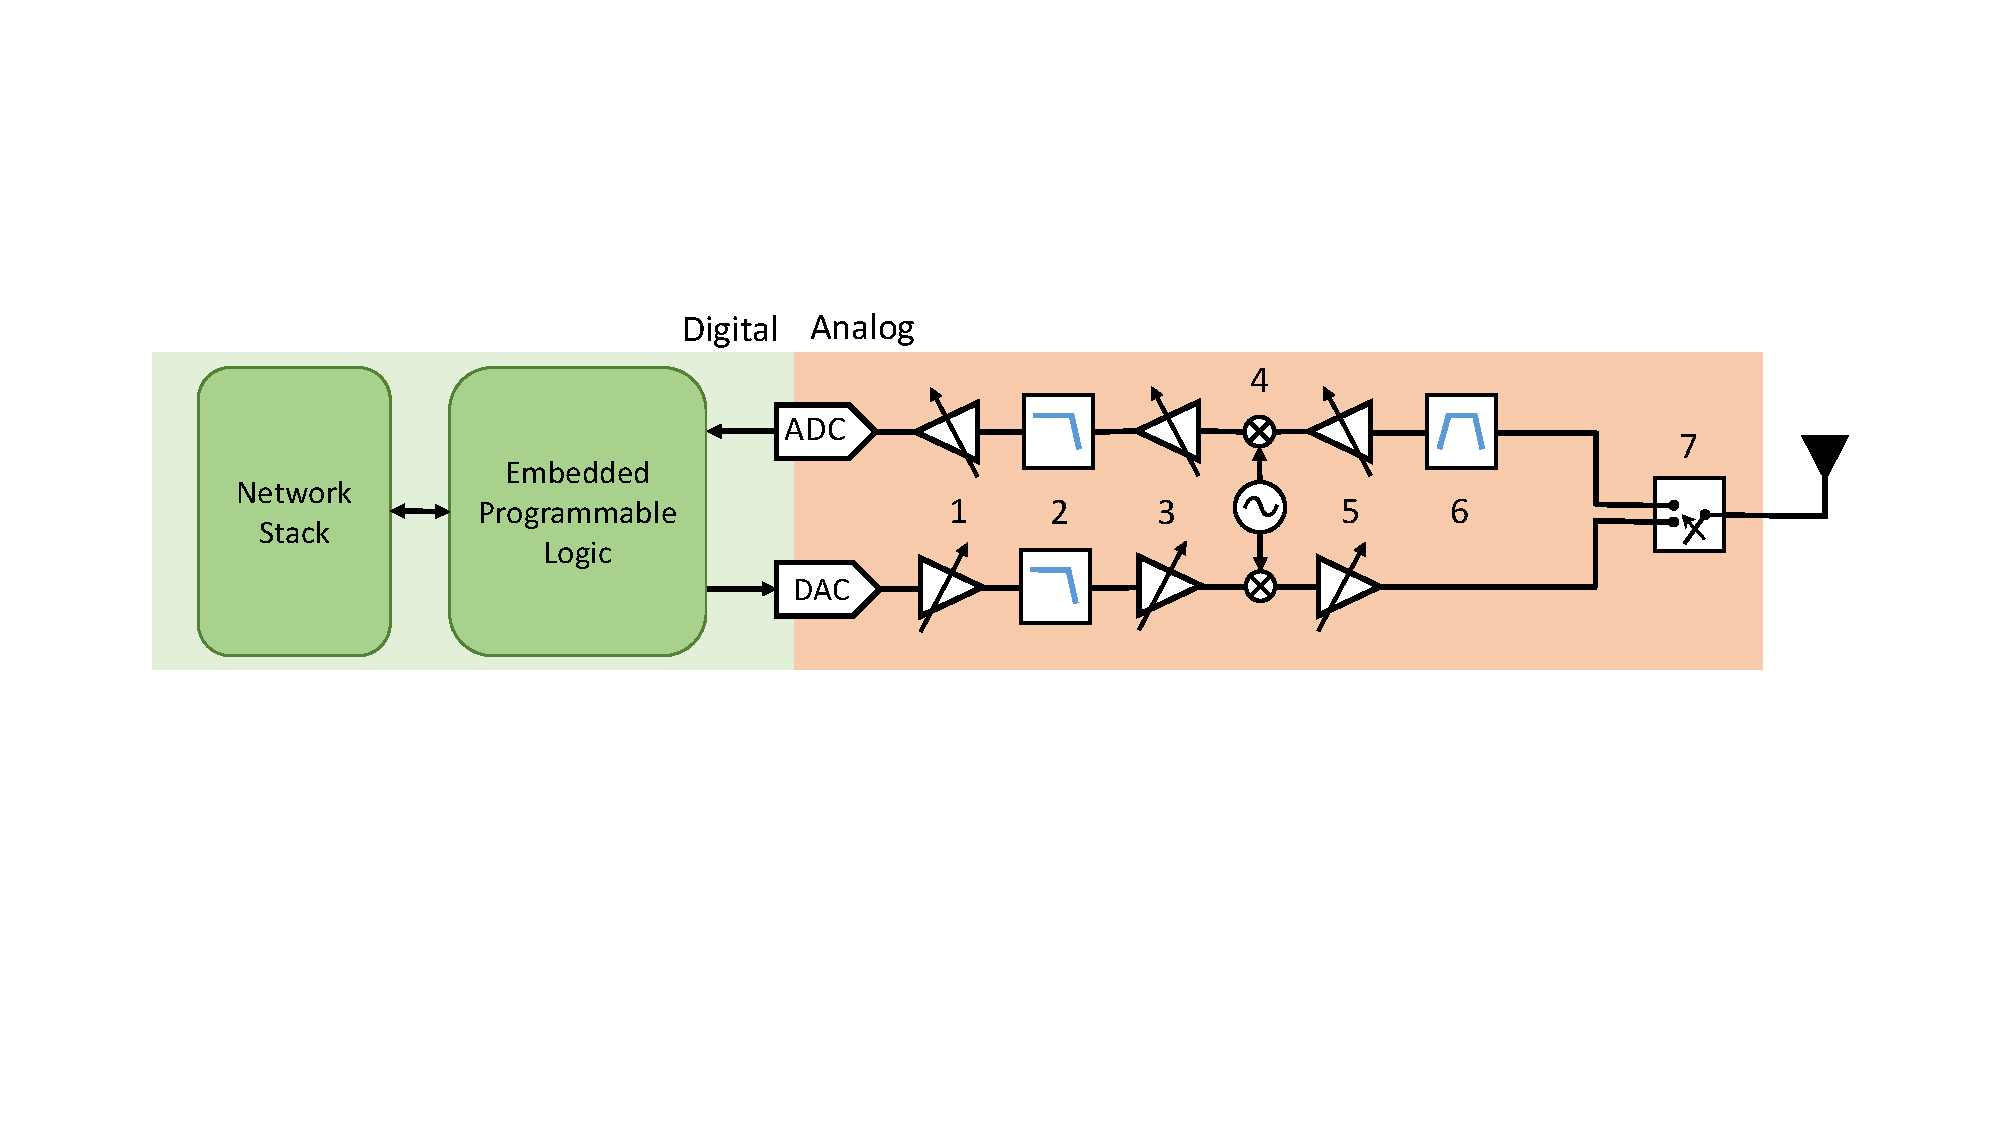
\includegraphics[width=1\linewidth]{./figs/agc/generic_sdr}
\caption{Block diagram of a generalized Software-Defined Radio system.}
\label{fig_sdr_ideal}
\end{figure}

We present a generalized block diagram model of a single-radio \ac{SDR} in Figure~\ref{fig_sdr_ideal}.
While implementations of \acp{SDR} vary, our model captures key components (from left to right) considered in this work and generalizes well to most commercial \ac{SDR} architectures:
\begin{itemize}
	\item \textbf{Network stack} - signal processing components with non time-critical functions; for example: user scheduling, priority queuing, or layer-2 routing.
	\item \textbf{Programmable logic} - signal processing components with time-critical or hardware-accelerated functions, specifically for networks layers 1 and 2; for example: gain control, digital pre-distortion, forward error correction.
	\item \textbf{Analog/Digital interface} - \acp{ADC} and \acp{DAC} provide the interface between digital and analog domains by converting digital samples to analog voltages and vice-versa.
	\item \textbf{Analog Gain Block (1)} - controls the amplitude of the signal entering or leaving the ADC/DAC.
	\item \textbf{Anti-aliasing filter (2)} - provides a low-pass filtering function on the analog signal to limit its information bandwidth to below the Nyquist sampling rate of the digital conversion step in order to avoid aliasing.
	\item \textbf{Analog Gain Block (3)} - controls the amplitude of the signal entering or leaving the analog mixer.
	\item \textbf{Frequency Up/Downconversion Mixing (4)} - a local center frequency, or \textit{carrier}, is multiplied by the analog signal to either up-convert or down-convert the signal to/from the RF frequency.
	\item \textbf{RF Gain Block (5)} - the input and output RF signal is amplified in order to meet the linearity or power budget requirements of the system's components.
	\item \textbf{Receive Band-Pass Filter (6)} - a band-pass filter limits the frequency content of the signal input to the receive radio chain in order to limit noise ingress and harmonic interference from strong out-of-band signals.
	\item \textbf{Transmit/Receive Switch (7)} - shares a signal antenna with the transmit and receive circuits; while this work generally considers \ac{TDD} protocols, this system component can be replaced with a frequency duplexer to support \ac{FDD} protocols, as well.
\end{itemize}

	This is by no means an exhaustive enumeration of the signal conditioning components present in all \ac{SDR} systems, but captures the important features needed for the techniques and systems in this work while being generic enough to apply across a wide range of commercial \ac{SDR} platforms.

	In addition, the division of functions between ``programmable logic'' and ``network stack'' blocks is a soft delineation made for ease of discussion.
	For the purpose of this work, we consider programmable logic to be an \ac{FPGA} or similar digital logic, whereas the network stack is implemented in embedded C or higher layer computer languages on a general-purpose processor.
	This division matches well-known experimental \ac{SDR} platforms like those mentioned in Section~\ref{sec_related_sdr}.

\subsection{Direct Sampling RF}
	As digital circuit integration and speed increases, a new \ac{SDR} paradigm is emerging in recent years that further reduces the amount of analog components necessary, shifting the dividing line between digital and analog domains in Figure~\ref{fig_sdr_ideal} nearly all the way to the antenna.
	``Direct sampling RF'' systems first used a combination of filtering and aliased sampling to directly sample RF signals without a down-conversion mixing step \cite{psiaki2005design}.
	More recently, increases in the integration and speed of digital circuits now permit direct sampling \acp{ADC} at RF frequencies without the drawback of aliased sampling \cite{xilinx2017rfsoc}.
	Although widespread use of direct sampling architectures will obviate the need for some of the analog components discussed in this thesis, key contributions of \ac{AGC}, environmental \ac{MU-MIMO} studies, and our protocol design remain unchanged.

%#######################################################
\section{Two Port Scattering Parameters}
\label{sec_scattering}

	In order to present some of our circuit design techniques, it will be necessary to be familiar with the definition and notation of normalized scattering, or S-parameters.
	The following discussion is a summary of the discussion and derivation by Yarman \cite{yarman2010design} and Orfanidis \cite{orfanidis2002electromagnetic} to describe a lossless two-port device.
	
\begin{figure}[h]
\centering
  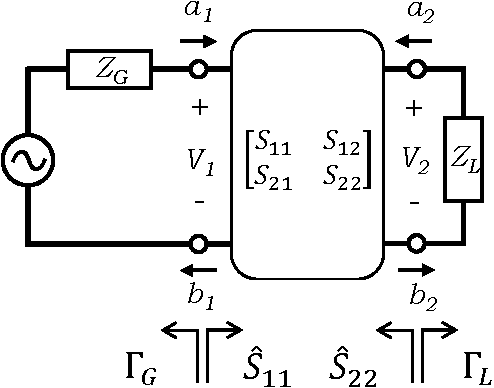
\includegraphics[width=0.4\linewidth]{figs/matching/general_2_port}   
    \caption{General diagram of a lossless linear 2-port device with scattering parameters.}
\label{fig_general_2_port}
\end{figure}
	
	Consider Figure~\ref{fig_general_2_port}, a linear two-port microwave device that is excited by a complex source or ``generator'' impedance $Z_G$ and terminated in a complex load impedance $Z_L$.
	Assuming it it lossless, it is possible to describe the two-port system by describing the relationship of any incident and reflected voltage wave characterized by the wave variables $a_i, b_i$, where the current is defined in the direction of the corresponding $a_i$ vector and the characteristic reference impedance of the system is $Z_0$.
\begin{align}
a_1 &= \frac{V_1+Z_0 I_1}{2\sqrt{Z_0}}  &a_2 = \frac{V_2+Z_0 I_2}{2\sqrt{Z_0}} \\
b_1 &= \frac{V_1-Z_0 I_1}{2\sqrt{Z_0}}  &b_2 = \frac{V_2-Z_0 I_2}{2\sqrt{Z_0}}
\end{align}
This results in a relationship between incident and reflected traveling waves:
\begin{align}
	b_1 &= S_{11}a_1 + S_{12}a_2 \\
	b_2 &= S_{21}a_1 + S_{22}a_2.
\end{align}
	The system of traveling wave equations forms a scattering matrix, $\mathbf{S}\in\mathbb{C}^{2\times2}$ for a two-port device, $\mathbf{S}\in\mathbb{C}^{4\times4}$ for a four-port device, etc, that completely characterizes the device's linear, lossless behavior.
	
	There are two important assumptions related to the use of S-parameters; the first is that each set of empirical S-parameter is measured within a system with arbitrary characteristic impedance $Z_0$.
	As a matter of convention, nearly all S-parameters are measured in reference to 50~$\Omega$ and we will assume that in the rest of this thesis.
	
	Second, S-parameters only capture \emph{linear} steady-state device behavior, and for this reason they are generally described as ``small-signal'' parameters. For example, as the input signal power to a two-port amplifier is increased close to the IP1dB point, or the point where the amplifier becomes saturated and the output power decreases by 1~dB from ideal, non-linear behavior will be observed, requiring ``large-signal'' design techniques like load-pull analysis.
	Quaglia and Cripps present an excellent discussion of recent developments and models for power amplifiers operating in the saturated regime \cite{quaglia2017reappraisal}.
	We instead focus on linear operating conditions and small-signal designs for our system in order to preserve the simplicity of each radio chain within a complex many-antenna system, leaving energy efficiency optimization to future work.

For the system in Figure~\ref{fig_general_2_port}, it is also useful to define generator and load \emph{reflection coefficients} that describe the portion of a reflected incident wave with characteristic reference impedance $Z_0$ into a load.
\begin{equation}
\Gamma_G = \frac{Z_G - Z_0}{Z_G + Z_0},~~~ \Gamma_L = \frac{Z_L - Z_0}{Z_L + Z_0}
\end{equation}

	In this work, we will use the $\hat{(\cdot)}$ notation to indicate a reflection coefficient that is cascaded into a non-reference impedance.
	For example, $\hat{S}_{11}$ in Figure~\ref{fig_general_2_port} is the reflection coefficient of the active two-port terminated in an arbitrary load impedance $Z_L$ and can be written:
\begin{equation} \label{eq_}
\hat{S}_{11}=S_{11}+\frac{S_{12}S_{21}\Gamma_L}{1-S_{22}\Gamma_L},
\end{equation}
where in the case of $Z_L = Z_0 = 50~\Omega$, we see that this reduces to $\hat{S}_{11} = S_{11}$.
	Similarly, we can see that:
\begin{equation}
\hat{S}_{22}=S_{22}+\frac{S_{21}S_{12}\Gamma_G}{1-S_{11}\Gamma_G}.
\end{equation}

	We now have the tools needed to address the broadband power transfer network design problems presented in Section~\ref{sec_wurc_pa_design}.
	

%###########################################################
\chapter{Architectures for Large-Scale TVWS Systems}
\label{sec_wurc}

	% WURC Hardware Introduction
\section{Introduction}
\label{sec_hw_intro}

	When \ac{TVWS} radio spectrum was first released for unlicensed use, the only systems that were available for operation on this band were early prototypes from Microsoft \cite{yuan2007knows} and Adaptrum \cite{ko2014television}, as well as a few other frequency-shifted single-radio, single-carrier modulation systems from several vendors \cite{ko2014television}. 

	In fact, we evaluate the performance of our own prototype legacy \ac{SISO} \ac{TVWS} system in Section~\ref{sec_siso_tvws} and show that while propagation of 802.11-like \ac{TVWS} systems is much improved compared to similar 802.11 networks operating in 2.4 and 5.8~GHz \ac{ISM} bands, system performance is significantly decreased due to the limited practical channel bandwidth available in \ac{TVWS}.\footnote{It was only in 2015 that final rules were issued by the FCC that enabled \ac{TVWS} systems to bond multiple 6~MHz TV channels within the United States \cite{fcc2015ro}.}
		
	At the time, no radio platform existed that: 1) allowed us to transmit at 1~Watt or greater within \ac{TVWS} bands; 2) allowed access to the \ac{PHY} layer for \ac{CSI}, precoding, and modification of the \ac{PHY} itself; and most importantly, 3) could be configured for large-scale, real-time, and \emph{mobile} \ac{MU-MIMO} operation.
	
	% WURC Prototypes
\begin{figure}[ht]
\centering
  	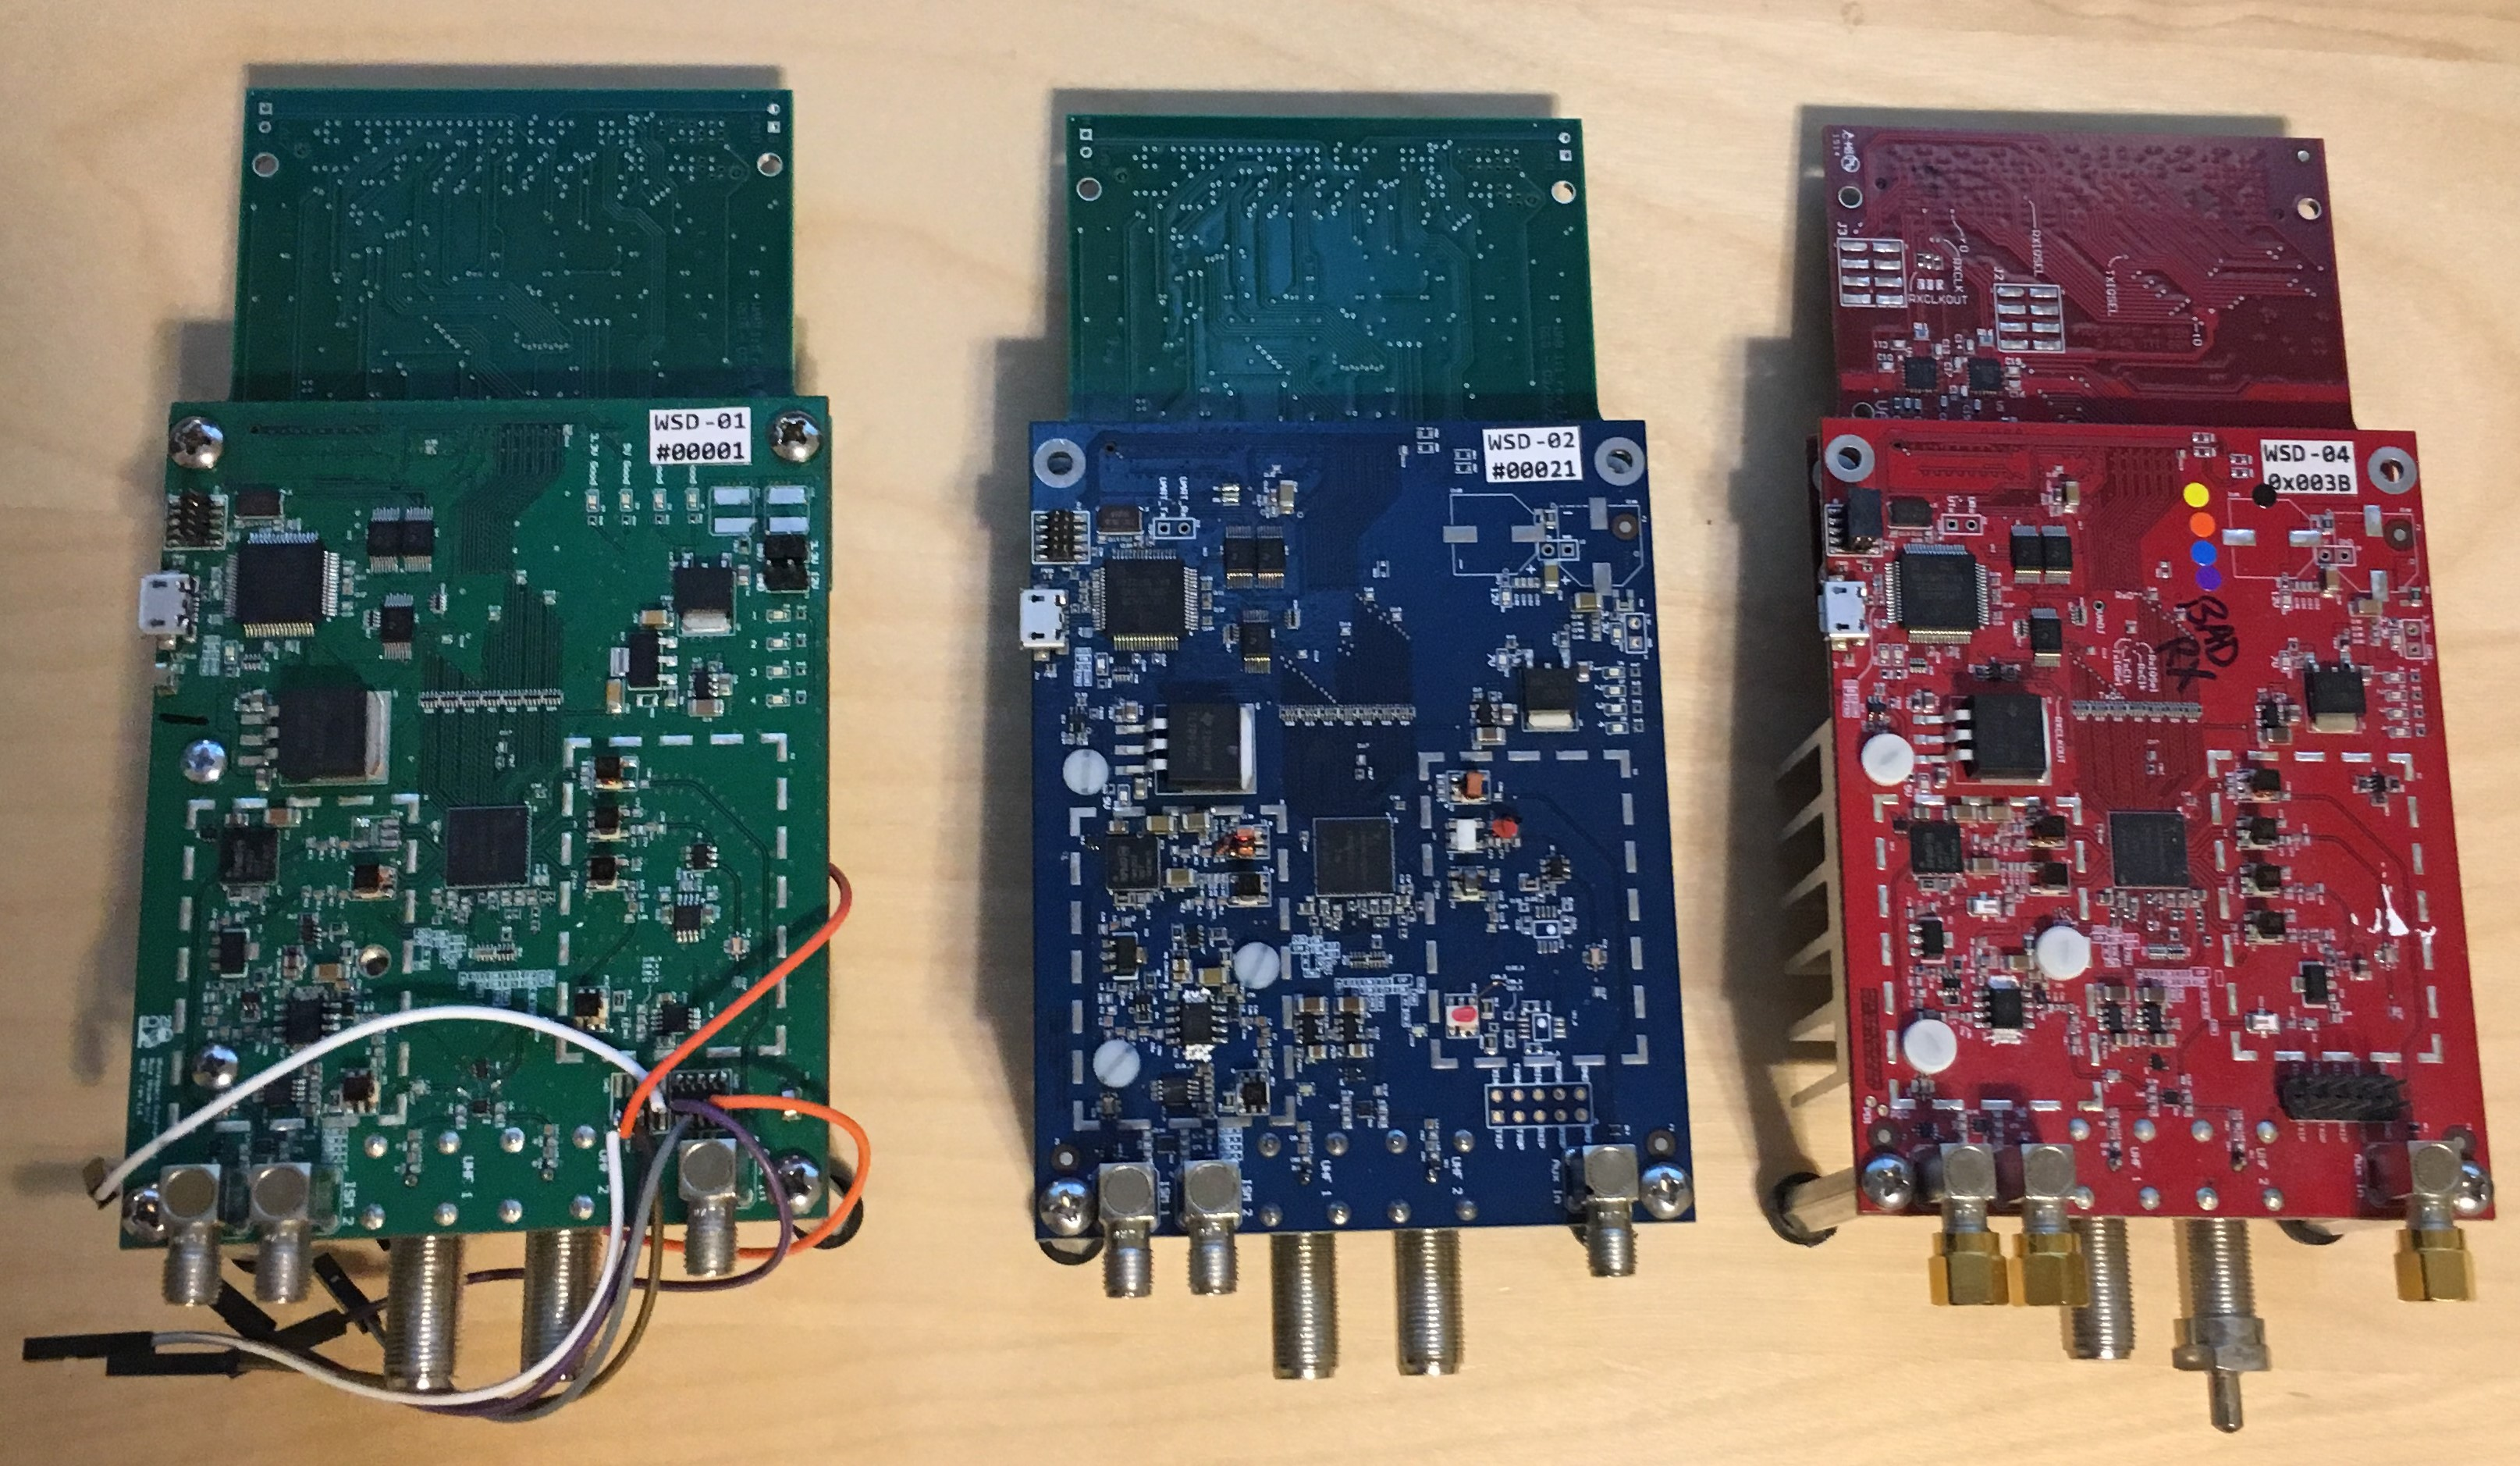
\includegraphics[width=1\linewidth]{figs/wurc/wurc_versions}   
   	\caption{Three revisions of the Wideband UHF Radio Card (WURC) prototype.
	\label{fig_wurc_versions}}
\end{figure}

	Therefore, in this chapter, we seek to design, implement, and test a new radio system that meets the above criteria for providing broadband connectivity over \ac{TVWS} channels.
	
	To this end, we present the \acf{WURC}, the first software-defined radio platform that implements 802.11af-like operation and \ac{MU-MIMO} beamforming \cite{WURC} (Figure~\ref{fig_wurc_versions}).
	When implemented in a larger system, \ac{WURC} is able to leverage an unprecedented tuning range for \ac{MU-MIMO} systems between 50 - 5875~MHz, enabling direct comparison of key \ac{MU-MIMO} performance metrics across \emph{two octaves} of radio spectrum.
	
	In order to realize this new experimental platform, we had to solve several key physical layer design challenges to enable agile, wideband operation, fast transit/receive switching required for the 802.11 \ac{DCF} protocol, and distributed clock and timing synchronization issues that limited the scalability of our system in particular and \ac{MU-MIMO} systems in general.
	
	These solutions are implemented on a new, modular PCB-based \ac{SDR} platform shown in Figure~\ref{fig_wurc_versions} that we designed, manufactured, and tested. Over 50 \ac{WURC} systems were manufactured and used in over a dozen research labs around the world for \ac{TVWS} system prototyping.
		
	This hardware platform was operated with an extensive and modular software command and control library that leverages the open-source WARP project to implement its \ac{PHY} rapid-prototyping experimental framework and real-time 802.11af-like communications framework \cite{warpProject}.

	%We first present a high-layer overview of \acp{WURC} modular architecture and construction, discuss the various \ac{PHY} design challenges and solutions we develop for \ac{WURC}.
	After describing the basic \ac{WURC} radio module, we will present several \ac{MU-MIMO} experimental platforms built with \ac{WURC} that enable us to achieve our large-scale \ac{TVWS} system design goals.


%##############################################################################
\section{WURC High-Level System Design}
\label{sec_wurc_module}

	\ac{MU-MIMO} systems generally require a large number of transmit and receive RF chains on the \ac{AP} to generate multiple spatial streams; these radios must be coherent (\emph{i.e.} share the same RF reference clock).
	In addition, a large number of distributed \ac{STA} nodes are required to serve as the clients to the \ac{AP}.
	Given that we wished to implement the complete 8x8 \ac{MU-MIMO} 802.11af standard with accessibility and programmability across the entire network stack, we decided to implement our own \ac{SDR} platform, \ac{WURC} that could be produced in large numbers.

% WURC hardware key features
\begin{figure}[ht]
\centering
  \includegraphics[width=1\linewidth]{figs/wurc/wurc_detailed_components}   
    \caption{A Wideband UHF Radio Card (WURC) with sections labeled.}
\label{fig_wurc_hw_diagram}
\end{figure}

	\ac{WURC} is a software-defined radio daughter-card, designed to present an abstracted 12-bit quadrature I/Q parallel interface and a serial control console to the host system.
	By designing each \ac{WURC} board as a self-calibrating, self-configuring radio head, we simplified the system architecture and made each unit modular.
	The layout and various important features of the \ac{WURC} \ac{SDR} module can be seen in Figure~\ref{fig_wurc_hw_diagram}, where notably a 50~$\Omega$ port for 2.4~GHz \ac{ISM}-band operation and a 75~$\Omega$ port for UHF-band operation are the primary antenna interfaces.
	
	We designed \ac{WURC} to implement the \textit{direct-conversion} \acf{FPRF} LMS6002D system from Lime Microsystems \cite{lime2012lms6002d}, which integrates frequency synthesis, quadrature digital/analog conversion, baseband filters, RF mixing, and programmable gain controls into a single integrated circuit.
		This minimizes size, implementation complexity, and energy-consumption of the radio transceiver chain while providing significant flexibility regarding analog RF properties.
	The LMS6002D is configured through a 4-wire serial interface into an 8-bit register space.
	In order to simplify the management of a large number of radio chains,  \ac{WURC} is designed to be modular, with calibration/control libraries and board-dependent calibration tables stored locally on each daughter-card on a Texas Instruments LM3S5R36 microcontroller \cite{ti2012stellaris} and controlled through a simplified \ac{UART} interface.
	This eases the requirements for integration with a host platform and makes the radio daughter-cards completely interchangeable.
	A simplified block diagram showing input and output data paths is shown in Figure~\ref{fig_wurc_block_diagram}.
	
	Some of the important system parameters that will be used in this thesis are available in Table~\ref{tab_wurc_specs}; additional hardware details can be found in the relevant hardware specification sheets \cite{lime2012lms6002d, ti2012stellaris}.

% Table generated by Excel2LaTeX from sheet 'Sheet1'
\begin{table}[htbp]
  \centering
  \caption{Important system parameters for \acf{WURC}}
%\resizebox{0.6\textwidth}{!}{%
    \begin{tabular}{|lrl|}
    \toprule
    \rowcolor[rgb]{ .31,  .506,  .741} \multicolumn{1}{|c}{\textcolor[rgb]{ 1,  1,  1}{\textbf{Parameter}}} & \multicolumn{1}{c}{\textcolor[rgb]{ 1,  1,  1}{\textbf{Value}}} & \multicolumn{1}{c|}{\textcolor[rgb]{ 1,  1,  1}{\textbf{Unit}}} \\
    \midrule
    \rowcolor[rgb]{ .863,  .902,  .945} \multicolumn{1}{|c}{\textbf{RF Transceiver}} & \multicolumn{1}{c}{\textbf{LMS6002D} \cite{lime2012lms6002d}} &  \\
    \midrule
    Tuning Range & 50 - 3800 & MHz \\
    \midrule
    \rowcolor[rgb]{ .863,  .902,  .945} Output Power (UHF) & 30    & dBm CW \\
    \midrule
    Output Power (ISM) & 27    & dBm CW \\
    \midrule
    \rowcolor[rgb]{ .863,  .902,  .945} ADC Bits & 12    & bits \\
    \midrule
    ADC Sampling Rate & 40    & MSps \\
    \midrule
    \rowcolor[rgb]{ .863,  .902,  .945} SFDR  & 60    & dBc \\
    \midrule
    DAC Bits & 12    & bits \\
    \midrule
    \rowcolor[rgb]{ .863,  .902,  .945} DAC Sampling Rate & 40    & MSps \\
    \midrule
    SPI Bus Rate & 50    & MHz \\
    \midrule
    \rowcolor[rgb]{ .863,  .902,  .945} \multicolumn{1}{|c}{\textbf{Microcontroller}} & \multicolumn{1}{c}{\textbf{TI LM3S5R36} \cite{ti2012stellaris}} &  \\
    \midrule
    Processor & ARM Cortex-M3 & - \\
    \midrule
    \rowcolor[rgb]{ .863,  .902,  .945} Clock Speed & 80    & MHz \\
    \midrule
    Debug Interface & Micro-USB, JTAG & - \\
    \midrule
    \rowcolor[rgb]{ .863,  .902,  .945} SPI Write Speed & 40    & MHz \\
    \midrule
    SPI Read Speed & 10    & MHz \\
    \bottomrule
    \end{tabular}%
%}
  \label{tab_wurc_specs}%
\end{table}%


% WURC block diagram
\begin{figure}[p]
\centering
  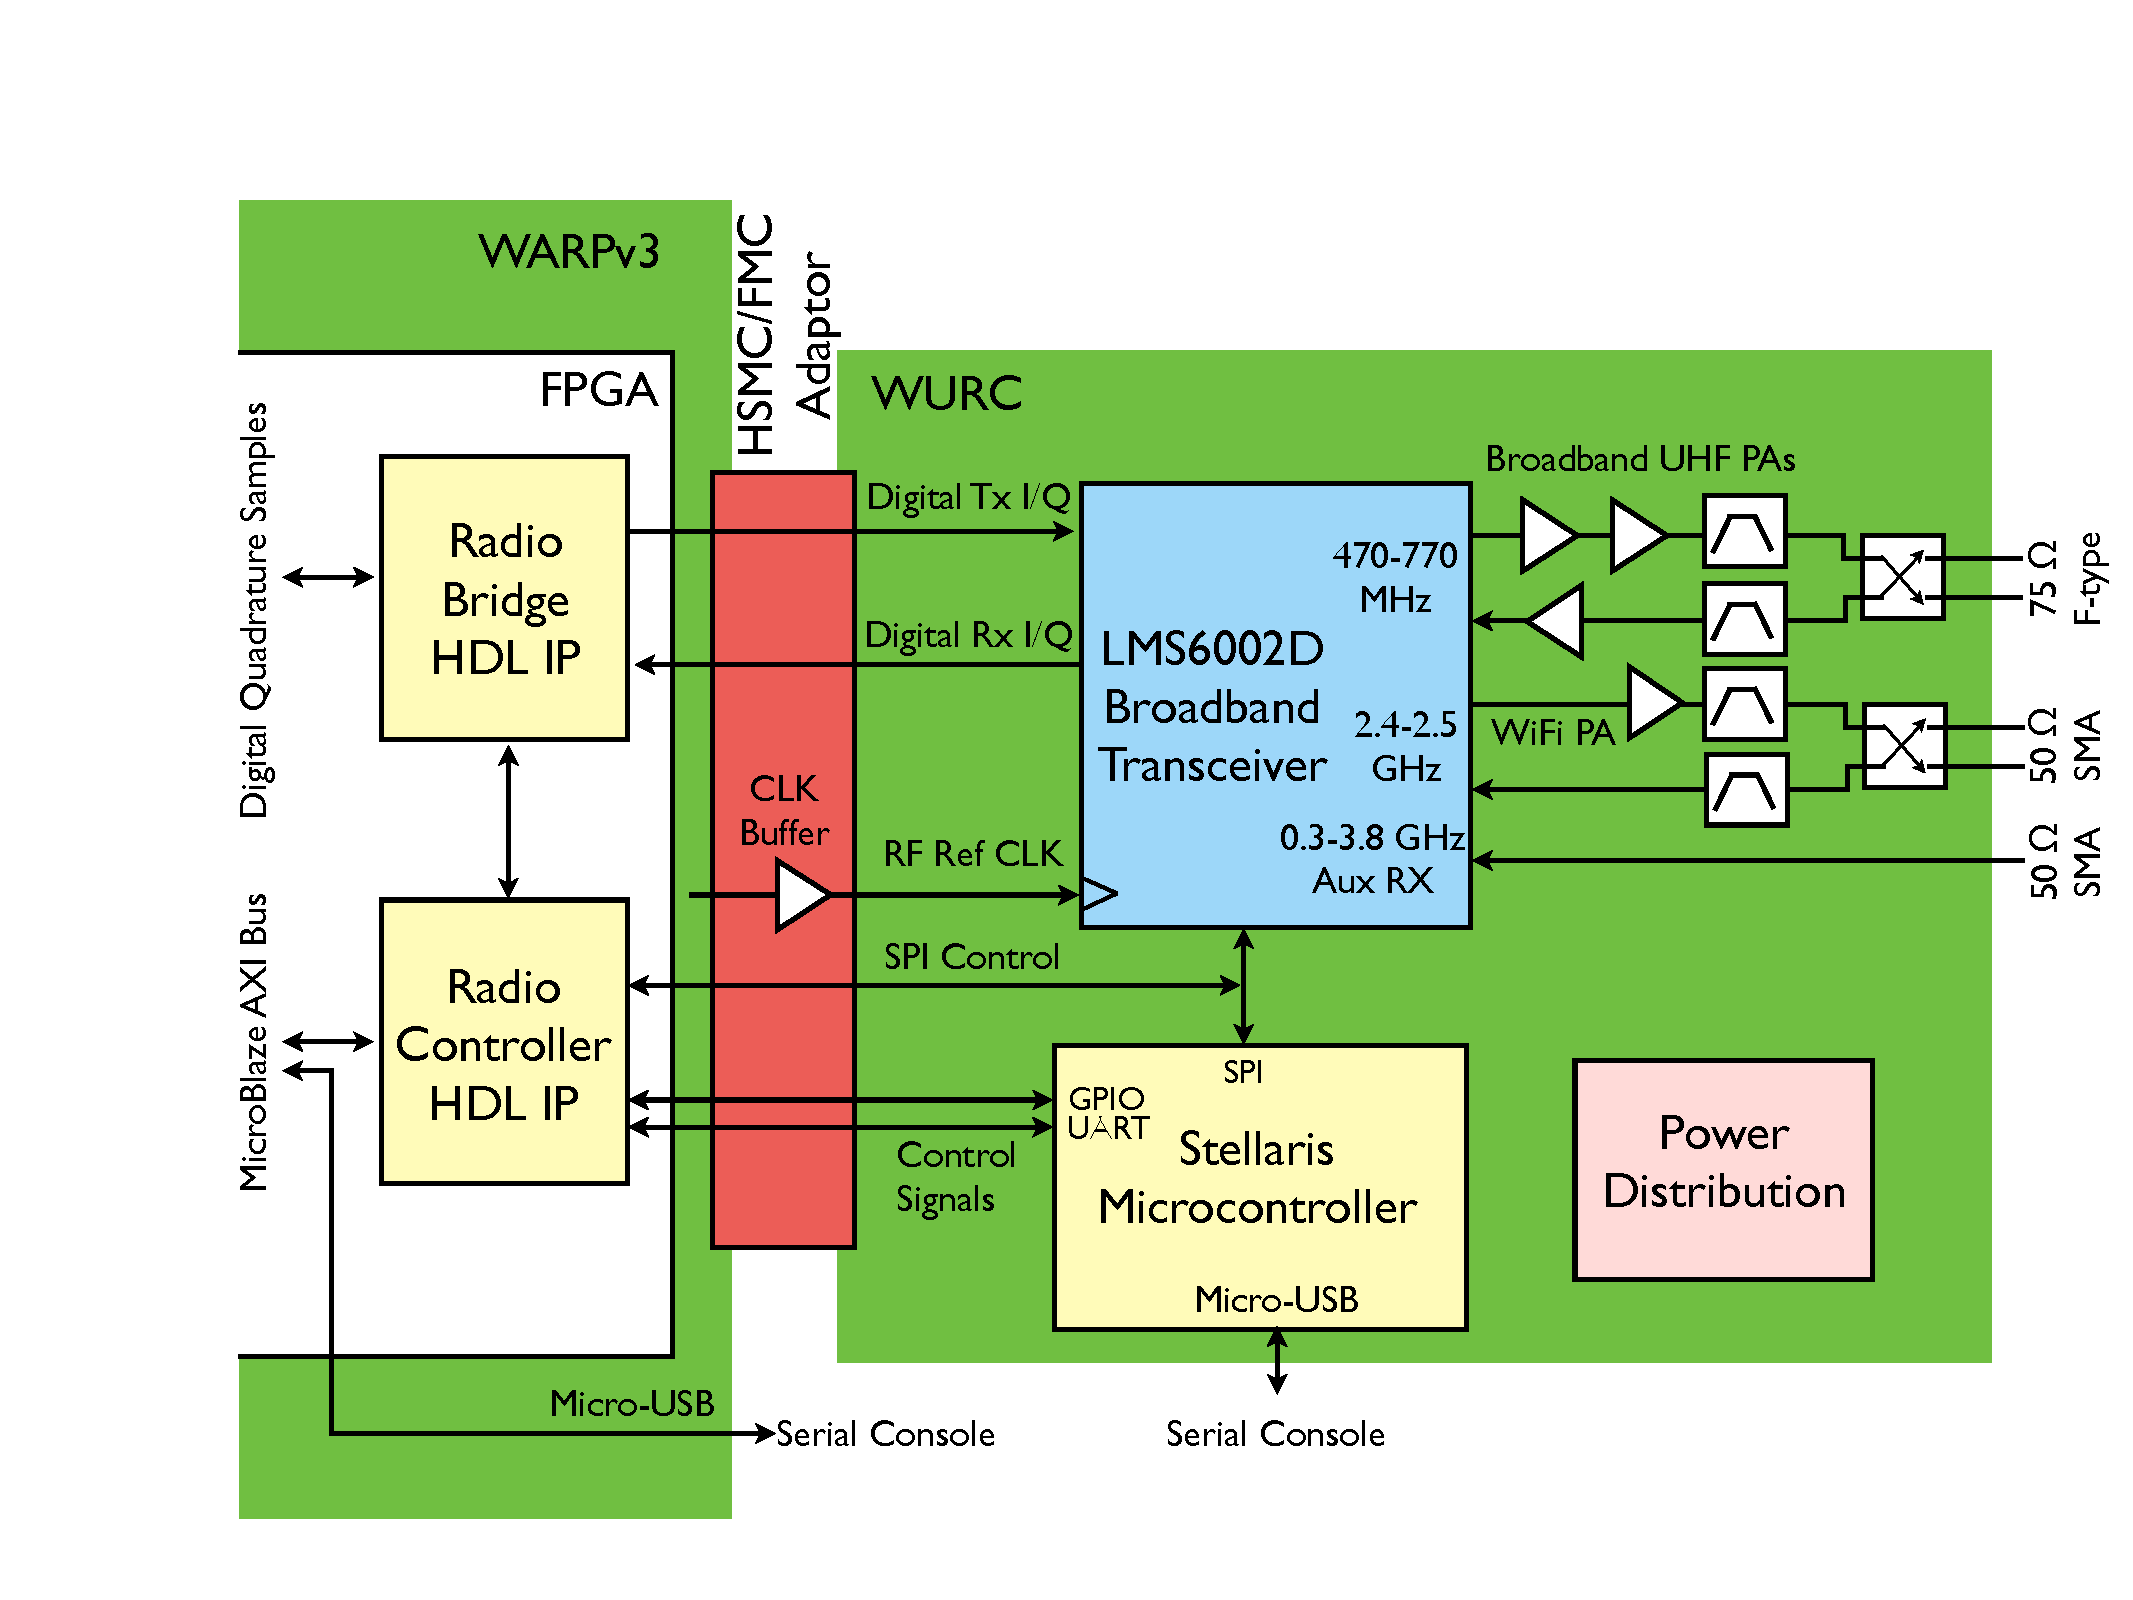
\includegraphics[width=0.7\linewidth]{figs/wurc/WARP_WURC}   
    \caption{Block diagram of WURC module on a host WARPv3 board.}
\label{fig_wurc_block_diagram}
\end{figure}

% WURC block diagram
\begin{figure}[p]
\centering
  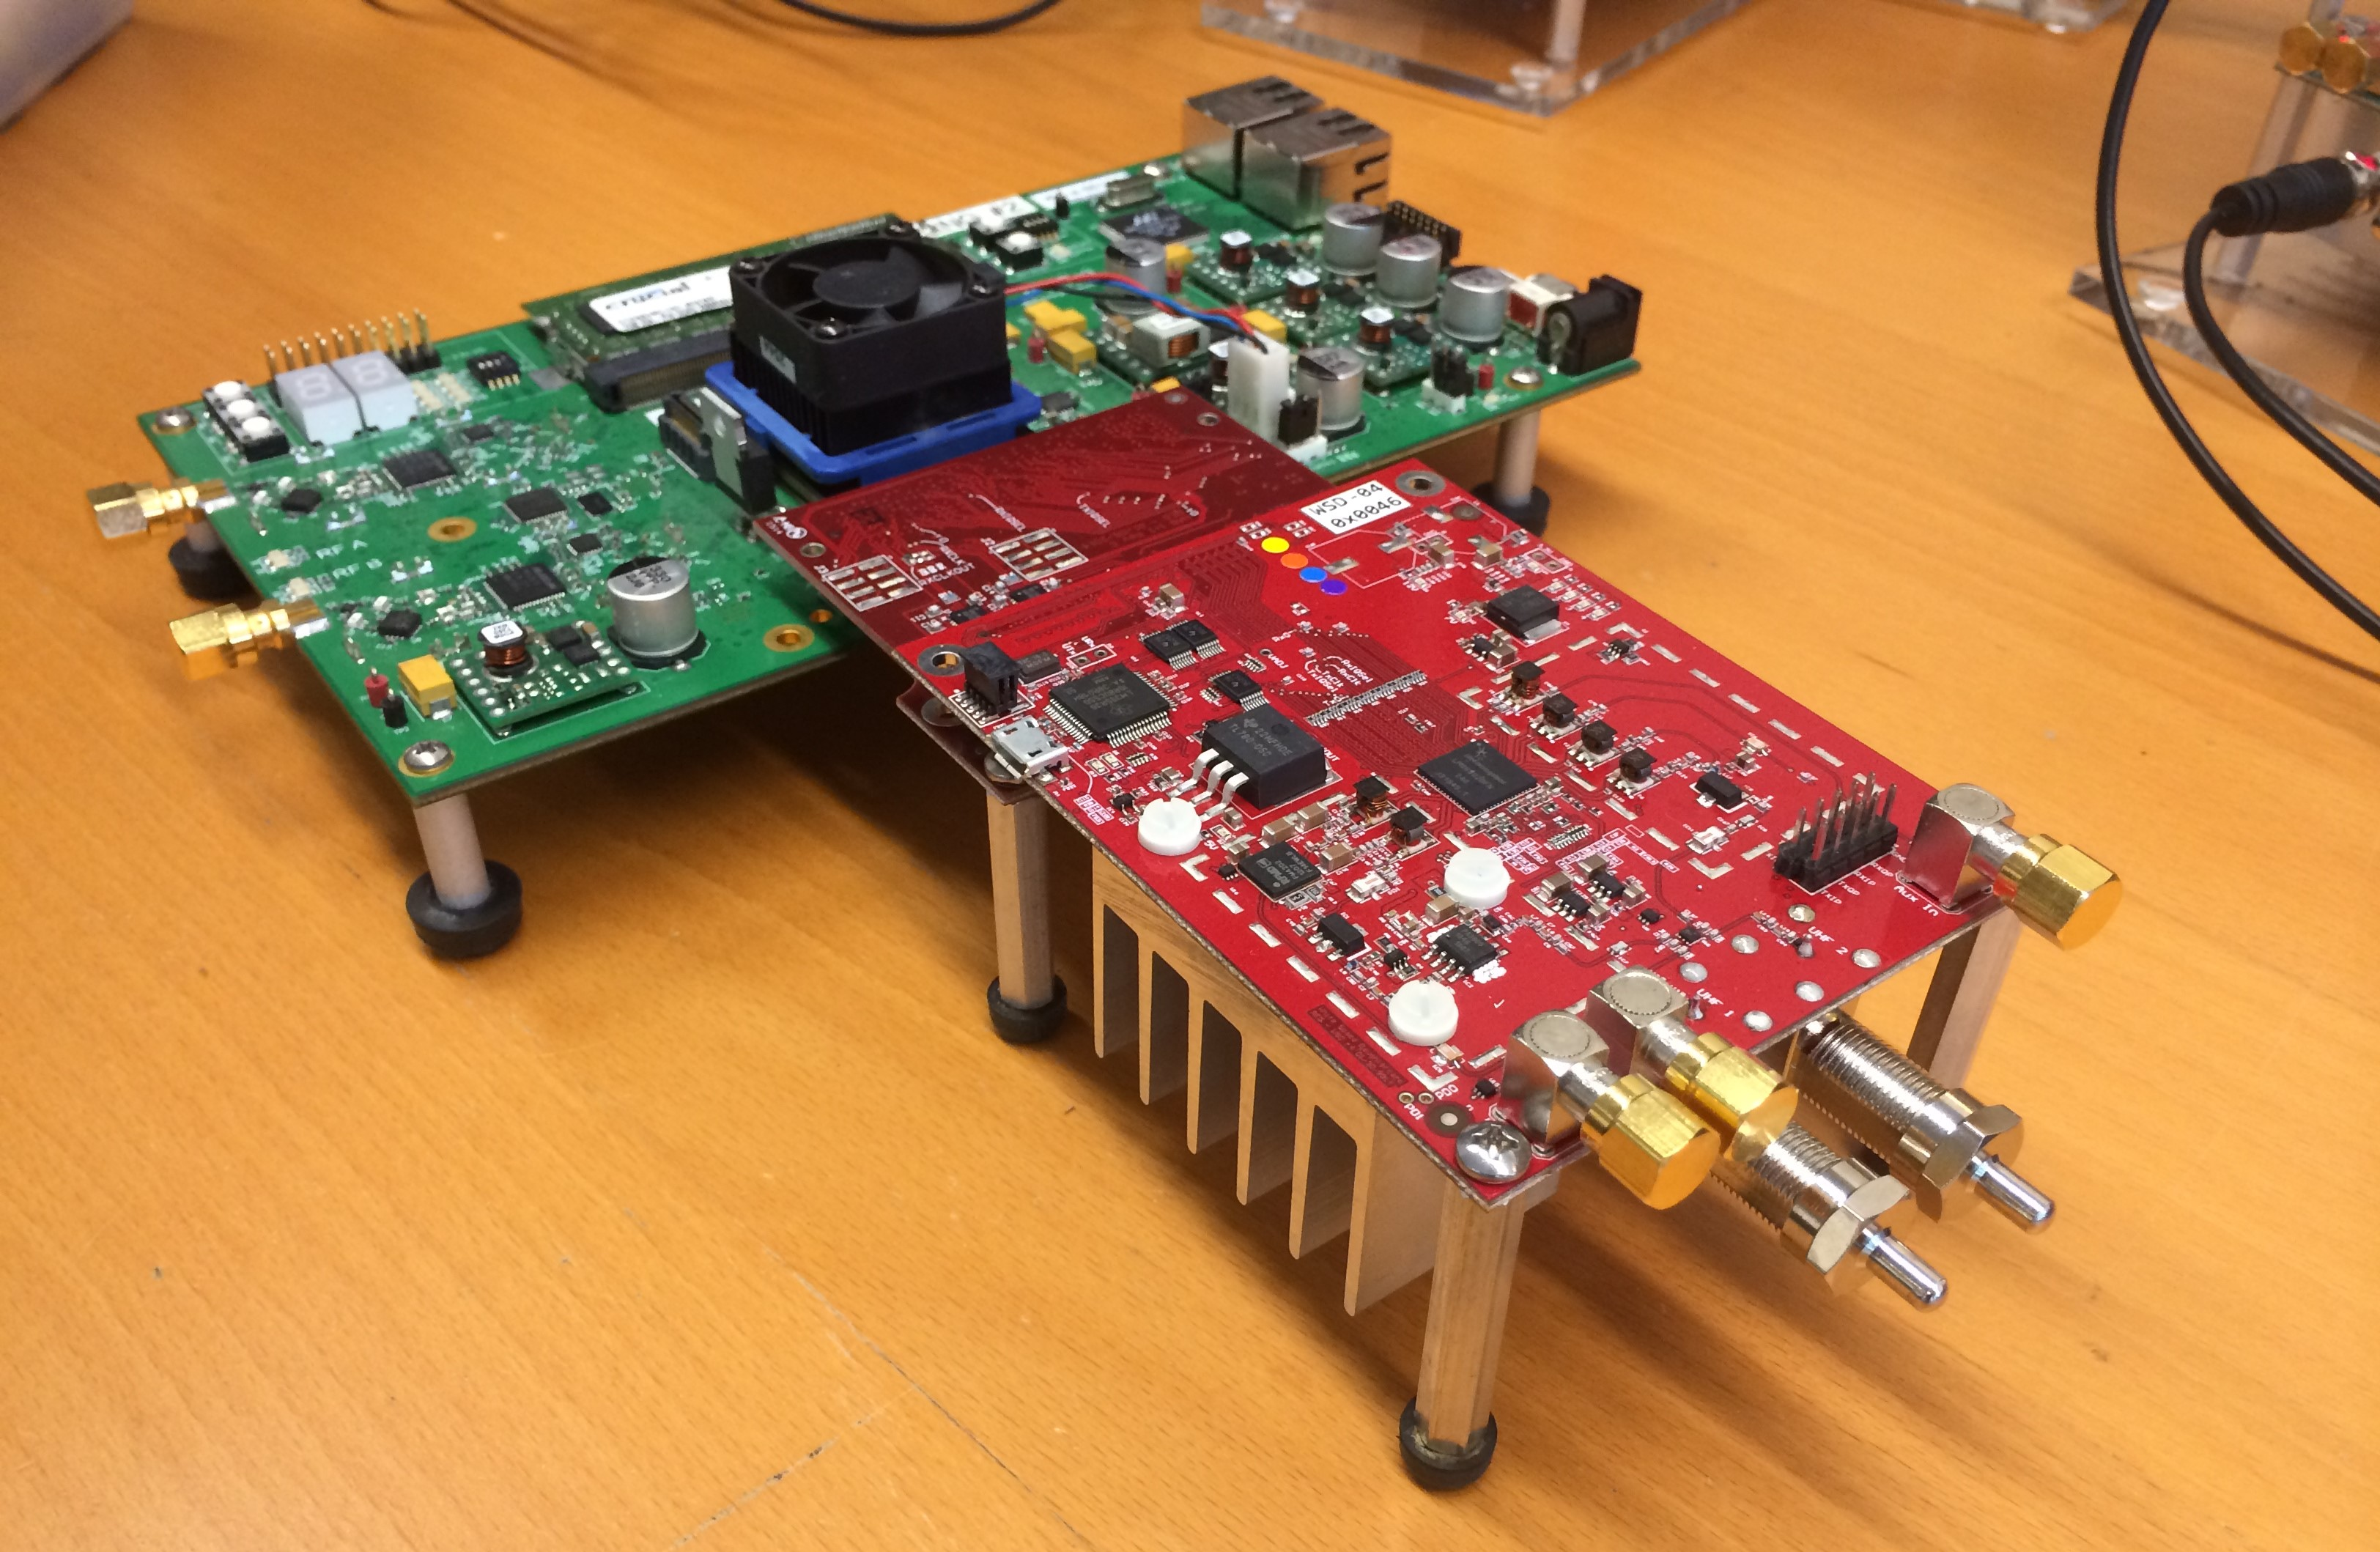
\includegraphics[width=0.7\linewidth]{figs/wurc/wurc_platform_rev_a_warp}   
    \caption{WARPv3 SDR platform, HSMC/FMC adaptor, and WURC SDR platform.}
\label{fig_warp_wurc_hw}
\end{figure}

	\ac{WURC} physically connects to a host via an HSMC or FMC (with custom adapter board) daughter-card slot, and provides a 12-bit digital baseband quadrature interface to the host system (Figure~\ref{fig_wurc_block_diagram}).
	This permits in-field reconfiguration of RF analog parameters such as channel bandwidth and center frequency between 300-3800 MHz, though the analog transmit and receive paths are currently optimized and calibrated for transmissions between 470-798 MHz on the UHF antenna ports, and 2400-2500 MHz on the ISM antenna ports.

	The daughter-card is powered by the 12V HSMC standard voltage rail, with all additional voltages and power filtering circuits contained on the daughter-card.

	We designed and tested fast-switching control circuits on the discrete amplification stages that allow the system to operate as a \ac{TDD} transceiver with a switching time of less than 7~$\mu$s, or an \ac{FDD} transceiver with independent transmit and receive fractional-N frequency synthesizers.
	Since our primary interest was to operate the \ac{WURC} as a \ac{TDD} 802.11af radio, we designed in two RF ports, one transmit/receive and one dedicated receive, which would allow the addition of an external duplexer for \ac{FDD} operation to a single antenna, if desired.
	For the rest of this thesis, we will focus on \ac{TDD} applications.
	
\subsubsection{WARP Framework Integrations}
\label{sec_warp_mods}

	WARPv3 is an open-source hardware platform for prototyping \ac{SDR} systems with a large Xilinx Virtex-6 LX240T FGPA, transceivers for 2.4 and 5.8~GHz ISM-bands, software reference designs, MATLAB integration \cite{warpProject}, and most importantly, a VITA 57.1 FMC expansion connector \cite{samtec2018vita}.
	With an intermediate adaptor \ac{PCB} that we designed and manufactured to translate between the HSMC and FMC mezzanine connector standards, we are able to interface our \ac{WURC} daughter-card to a host WARPv3 system shown in Figure~\ref{fig_warp_wurc_hw}.
	In the WARPv3 \ac{FPGA}, we multiplex radio control signals and digital quadrature I/Q streams between the built-in ISM-band radios and WURC's UHF transceivers.

	A standards-compliant 802.11 \acf{MAC} and \acf{PHY} implementation has been developed for the WARPv3 platform \cite{warp80211}, which we use as a starting point for our real-time 802.11af implementation \cite{flores2013ieee80211af}.
	From the perspective of the WARP 802.11 digital baseband, the analog front-end is transparent, which allows an interchangeable \emph{analog} \ac{PHY} to be used with the same digital MAC/PHY for fair comparison.
	This is especially useful for MU-MIMO comparison studies across ISM bands as this re-used of the digital MAC/PHY controls for a large number of variables in the radio chain.

\subsubsection{Adjustable Channel Bandwidth}
\label{sec_warp_chan_bw}

	The 802.11 reference design operates by default in a 20~MHz channel bandwidth.
	In order to enable a UHF transmission to fit within one or two contiguous UHF channels of 6~MHz, we modify the 802.11 reference design to operate at 10 and 5~MHz channel bandwidths in compliance with the 802.11af standard \cite{warp80211}.
	This is accomplished by reducing the data sampling rate by $\frac{1}{2}$ and $\frac{1}{4}$, respectively, with new programmable decimation filters added to the WARPv3 reference \ac{FPGA} design and adjusting \ac{MAC} timing parameters and receiver \ac{DSP} blocks to match.
	
		Now that we've presented the high-level overview of the designed \ac{WURC} \ac{TVWS} radio module, we will now dive in to some of the important \ac{PHY} problems and solution that were required to realize this platform before rounding out this chapter with a discussion of software architecture design for scaling from 1x1 up to 8x8 and larger \ac{MU-MIMO} arrays.

 % <-- introduction here
	%##########################################
\section{Broadband Power Transfer Networks}
\label{sec_wurc_pa_design}

%\rgnote{This is a brief of the content that will be presented here--I have models, simulations, and a discussion of the new design approach (and why alternative methods don't work). This is a contribution that first formulates a numerical optimization framework for wideband matching building on Yarman's real frequency techniques, and then solves it to produce a seed mathching circuit design. We show that although Yarman leaves off here, that is not sufficient to realize a practical solution and that additional parasitic models and empirical design techniques must be used to bring the design to realization. I'm cleaning up the plots and code to expand this section right now.}

	In order to operate as an opportunistic transmitter in the UHF band and adapt to various channel bandwidths, spectrum availability, and regulatory domains across the world, \ac{WURC} is designed to operate at arbitrary channel bandwidths from 1.5 - 28~MHz with center frequencies ranging from 470 - 700~MHz on its 75~$\Omega$ UHF antenna ports, and 2400 - 2500~MHz on its 50~$\Omega$ ISM antenna ports. 

	We target a design goal of radio output power up to 30~dBm from 470 to 700~MHz, the maximum conducted power to the antenna currently allowed by the \ac{FCC} in the United States for unlicensed operation within a single 6~MHz UHF channel \cite{flores2013ieee80211af}.\footnote{The 30~dBm limit is measured at the input RF connector to the antenna. \ac{FCC} regulation allows up to 36~dB \ac{EIRP} when including passive antenna gain. With antenna gain greater than 6~dB, the conducted power limit is decreased by 1~dB for each 1~dB of additional antenna gain in order to maintain a 36~dBm \ac{EIRP} maximum per 6~MHz channel. When channels are bonded, the total power budget for all channels is increased according to the total number of bonded channels \cite{fcc2015ro}.}
	The 2.4~GHz ISM transmit chain provides up to 27~dBm between 2400 - 2500~MHz.
	%The wide UHF frequency range presents a challenge for a high-power RF design since power amplifiers and their associated impedance matching networks are generally optimized for a narrow frequency band.

	By targeting nominal operation between 470 - 700~MHz, the \ac{WURC} analog front end utilizes a passband that is approximately $\frac{2\cdot(700-470)}{700+470}\cdot 100\% = 39.3\%$ wide, which is a significant design challenge.
	Intuitively, the wide 160~MHz channels for 802.11ac or 2.16~GHz for 802.11ad standards seem large, but they only represent a percent bandwidth of 3.1\% and 3.6\%, respectively, making their power transfer networks more simple.\footnote{Accurate physical modeling and parasitics are more of a concern at 5.8 and 60~GHz than is achieving a wide bandwidth power transfer match.}
	The efficiency of a \emph{passive} power transfer network will fundamentally trade off with the operational bandwidth of that network, as first proved by Fano for a simple RC capacitive load \cite{fano1950theoretical}.
	Fano's fundamental limit motivates the need to optimize the efficiency of the passive transfer network that delivers power to the various amplification stages of \ac{WURC}.
	As we will show, this process is non-trivial and requires multiple iterations utilizing various design techniques.

	In this section, we will first utilize real frequency techniques to construct an optimization problem and numerically solve for an ideal solution for the passive broadband power transfer network design.
	We will then show that this solution is inadequate to actually realize in a passive lumped element circuit, which will require us to develop empirical models of our circuit elements and layout to accurately capture parasitic circuit elements.
	This will finally allow us to synthesize a physical circuit realization that meets design goals.
	The circuit is manufactured, tested, and validated with consistent results that eventually match simulated results.

%%##################################################
%\subsection{Power Transfer Network Synthesis}
%\label{sec_match_synthesis}
%
%\rgnote{content snipped from paper follows, FIXME} 
%
%
%A common technique for designing high-power analog front-ends is to build multiple switched amplification and filtering chains, each optimized for a narrow band.
%However, when the system operating frequency range spans multiple octaves, space and cost constraints require that each chain support a wide range of frequencies.
%In the design of \ac{WURC}, we target two optimized transmit and receive chains for 470-698~MHz and 2400-2500~MHz, chosen because these two bands allow unlicensed operation and are invaluable for research and testing.
%
%
%
%Since the bandwidth of an RF chain is generally proportional to $\Delta f/f$, common techniques for designing and implementing discrete power transfer networks (e.g., multi-section Chebyshev transformers \cite{grebennikov2005rf}) either cannot meet design requirements for passband flatness or result in non-realizable circuits when applied to bandpass designs spanning a large frequency range like 470-698 MHz.

% ###################################
\subsection{Real Frequency Technique for Initial Circuit Synthesis}
\label{sec_dual_match}

%\rgnote{State the GEL dual matching problem here.}
%
%\begin{figure}[h]
%\centering
  %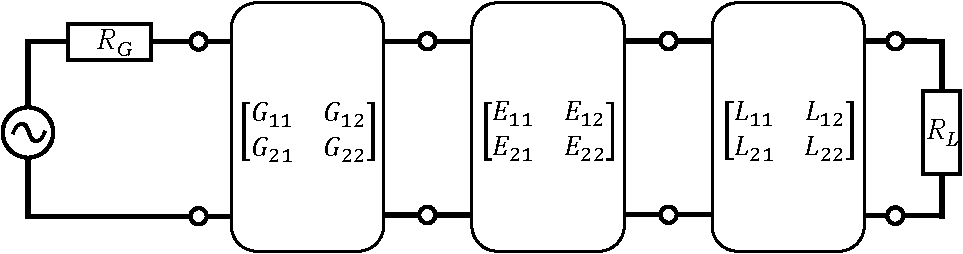
\includegraphics[width=0.67\linewidth]{figs/matching/matching_gel}   
    %\caption{Block diagram of dual matching problem with Darlington source and load representations.}
%\label{fig_matching_gel}
%\end{figure}

 	Several traditional analog design techniques can be used to design a passive matching network for amplifier circuits, such as an analytical conjugate match \cite{orfanidis2002electromagnetic} \S13, the direct design approach using the Smith Chart \cite{grebennikov2005rf} \S3.3, or prototype filter design \cite{grebennikov2005rf} \S10.7.	
	However, in the case that the desired passive matching network must match a complex real-world device over a large bandwidth, then these traditional design techniques become ``inaccessible'' \cite{yarman2010design, chen2015broadband}.
	Specifically, analytical and direct design techniques can yield physically feasible results for narrowband matches but produce negative-valued resistances, require the use of ideal transformers, or require very high-order circuits with a large number of components for wideband matches.
	Unfortunately, while useful for developing circuit theory, each of these outcomes is either not possible or extremely impractical to actually implement with a passive physical circuit.
	
	Instead, we utilize the real frequency matching technique proposed and developed by Carlin and Yarmin \cite{carlin1977new, carlin1983double, yarman1982simplified} which utilizes numerical methods to solve for a piecewise approximation to the reflection coefficient of the optimal matching network.
	The entire set of matching network S-parameters are determined from a series of identities and Belevitch factorizations of the single reflection coefficient \cite{yarman1982simplified}.
	Finally, an LC-ladder circuit can be realized with a simple lumped element passive circuit using long division(\cite{yarman2010design} \S9.7).
	We repeat this optimization for both the input and the output matching network for each amplifier component separately rather than using the cascaded gain stage approach proposed by Yarmin \cite{carlin1983double} for practical reasons: we find that physical circuit layout is improved when each amplifier component is individually matched to the system characteristic impedance rather than to each other, allowing arbitrary placement of the components.

% ######################
\subsubsection{Broadband Matching Problem Statement}
\label{sec_srft_problem_statement}
	
	Our objective is to maximize the \ac{TPG} of our chosen broadband amplifiers across the target band of operation utilizing only passive, lumped-element power transfer, or ``matching'' networks between the source \ac{SDR} transceiver, analog pre-amplifier and power amplifier stages, and the antenna.
	We choose to target a flat frequency response within the 470 - 700~MHz passband, thereby simplifying operation while maximizing the Bode-Fano bandwidth-efficiency tradeoff  \cite{bode1945network, fano1950theoretical}.
	
	The active amplifier circuits for the TQP3M9009 and RFPA3800 are represented by their de-embedded two-port S-parameter representations (Section~\ref{sec_scattering}) obtained from the component vendors and validated using evaluation boards for each component.
	In the case where the component S-parameter data are sampled at different frequency intervals, we observe that their real and imaginary components are individually smooth functions and therefore we can linearly interpolate the real and imaginary components separately with negligible loss in their S-parameter representation accuracy before recombining into a sequence of complex $\mathbf{S}[\omega_i]\in\mathbb{C}^{2\times 2}$ matrices indexed by uniform frequency intervals $\omega_i$.
	The original technique proposed by Carlin \cite{carlin1977new} also solved for the optimal ``break points,'' or arbitrary frequency points for representing the sampled reflection coefficients; however, we simplify the problem formulation by choosing uniform break points and oversampling substantially.
	Modern computational capabilities permit this luxury.
	
	Assuming a steady-state input stimulus and linear operating regime,\footnote{While our small-signal technique does not, in general, optimize the performance of the system when the amplifier becomes saturated, we claim first that energy efficiency was not one of our design goals, therefore operating the amplifier near saturation is not desired; and second, the design paradigm of many-antenna wireless systems is to \emph{reduce} the power budget of any single radio chain while relying on array beamforming gain to provide the link budget necessary for communication. Therefore, we always expect to operate this design in the amplifier's linear operating regime, which is where small-signal techniques excel.} the first stage amplifier system for optimization can be represented as in Figure~\ref{fig_matching_stage_1}.
	
\begin{figure}[h]
\centering
  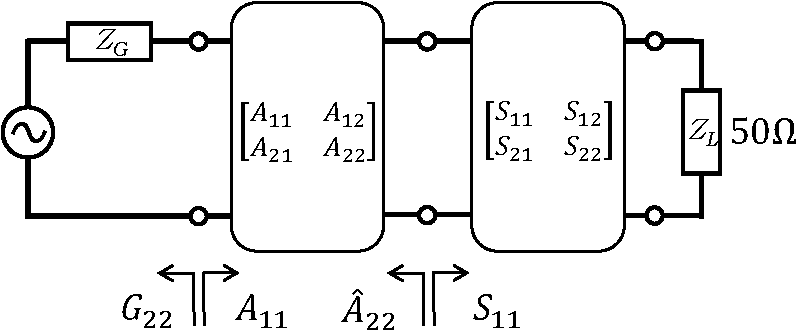
\includegraphics[width=0.67\linewidth]{figs/matching/matching_stage_1}   
    \caption{First stage of the dual matching problem with an active amplifier.}
\label{fig_matching_stage_1}
\end{figure}

	%In the first half of the optimization, we consider the partial system shown in Figure~\ref{fig_matching_stage_1}.
	Both the source impedance, $Z_G(\omega)$, and the amplifier itself, $\mathbf{S}(\omega)$, are parametrized with scattering parameters, allowing the complex frequency response of the amplifier to be represented with empirical data.
	For this stage, the load impedance is set to be purely resistive: $Z_L(\omega) = Z_0 = 50~\Omega$.

% ############### 
\subsubsection{Real Frequency Objective Function Stage 1}
\label{sec_srft_stage_1}

	With this simplification, our goal is to find the input matching network as a function of angular frequency, $\textbf{A}(\omega)$, that maximizes the flat \ac{TPG} of the active amplifier cascaded into a 50-$\Omega$ load, or formally:
	\begin{equation} \label{eq_stage_1}
		\argmax_{[\textbf{A}(\omega)]}{[T_1(\omega) - T_{01}]},
	\end{equation}
where the first stage \ac{TPG} is
	\begin{equation} \label{eq_stage_1_tpg}
		{T_1(\omega)} = |G_{21}|^2\frac{|A_{21}|^2}{|1-A_{11}G_{22}|^2\cdot|1-\hat{A}_{22}S_{11}|^2}|S_{21}|^2,
	\end{equation}
and the target flat \ac{TPG}, $T_{01}$, is set by the engineer.
	A reasonable value for $T_{01}$ can be more systematically determined by setting $T_{01}$ to the minimum value of the amplifier's \ac{MAG} within the band of interest and decreasing $T_{01}$ until an acceptable solution to Equation~\ref{eq_stage_1} is found.
	For an active amplifier in a nominal 50~$\Omega$ circuit, the \ac{MAG} for an unconditionally stable \cite{orfanidis2002electromagnetic} amplifier is defined as 
\begin{equation} \label{eq_mag}
T_{MAG} := \frac{|S_{21}|^2}{(1-|S_{11}|^2)(1-|S_{22}|^2)}.
\end{equation}

	In Equation~\ref{eq_stage_1_tpg}, we let $p:=j\omega$ and the unknown $\mathbf{A}(\omega)$ is completely determined by the polynomial
\begin{equation}	
\hat{A}_{22}(p) = \frac{h(p)}{g(p)} = \frac{h_np^n+\dotsb+h_1p+h_0}{g_np^n+\dotsb+g_1p+g_0}, \label{eq_belevich_poly}
\end{equation}
where the optimization is taken over just the coefficients of $h(p)$, since all other terms can be derived uniquely from $h(p)$ as shown by Yarman \cite{yarman1982simplified}.
	First, the solution matching equalizer is assumed lossless, therefore we restrict solutions to those that obey the lossless criterion $$g(p)g(-p)=h(p)h(-p)+(-1)^k p^{2k} ~>~ 0 ~\forall p,$$
which provides the means to derive $g(p)$ from $h(p)$. %G(p^2)=
	The remaining terms are also derived as:\footnote{There is a typo in \cite{yarman2010design} with incorrect derivation of $A_{11}(p)$. The equations given here are correct and verified with working examples.}
\begin{align}
	A_{12}(p) &= A_{21}(p) = \textpm \frac{p^k}{g(p)} \\
	A_{11}(p) &= -(-1)^k\frac{h(-p)}{g(p)}.
\end{align}

	The number of reactive circuit elements is set implicitly by allocating the initial polynomial solution $h(p)$ with length $n$.
	The order of the zero of the transmission coefficients $A_{12}(p)$ at DC is also set to $k \in \mathbb{Z} \geqslant 0$ by the engineer, thus providing all the remaining unknowns and allowing the optimization to continue.
	In our case, we set $k=0$ in order to avoid additional components needed to produce zeros at DC; this produces a lowpass circuit.
	This could introduce some inefficiency in our synthesized matching circuit since the Bode-Fano limit suggests zeroing gain outside of the desired passband \cite{bode1945network, fano1950theoretical}, however we find that the tradeoff in reducing the number of components to realize the circuit to be worth it.
	
% ############### 
\subsubsection{Real Frequency Objective Function Stage 2}
\label{sec_srft_stage_2}

\begin{figure}[h]
\centering
  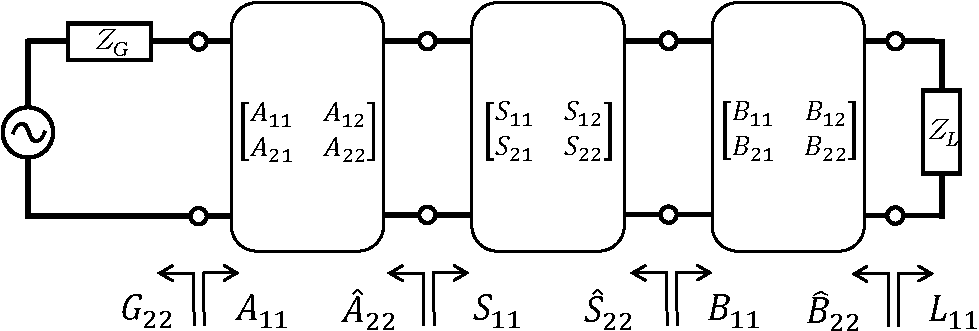
\includegraphics[width=0.8\linewidth]{figs/matching/matching_stage_2}   
    \caption{Second stage of the dual matching problem with an active amplifier.}
\label{fig_matching_stage_2}
\end{figure}

	Once the input matching equalizer has been synthesized, we then change the load impedance from a nominal $50~\Omega$ to $Z_L(\omega)$, which may be a constant scalar value represented by its Darlington 2-port equivalent reflection coefficients \cite{yarman2010design} or may be specified empirically by measured or modeled 2-port S-parameters $\textbf{L}(\omega)$.
	We fix $\textbf{A}(\omega)$ to the optimal value found for Equation~\ref{eq_stage_1} and define a new optimization objective function for the cascaded \ac{TPG} for the system extended in Figure~\ref{fig_matching_stage_2}:
\begin{equation} \label{eq_stage_2}
	\argmax_{[\textbf{B}(\omega)]}{[T_2(\omega) - T_{02}]},
\end{equation}
where the second stage \ac{TPG} is
\begin{equation} \label{eq_stage_2_tpg}
	{T_2(\omega)} = \overbar{T_1}(\omega)\frac{|B_{21}|^2}{|1-B_{11}\hat{S}_{22}|^2\cdot|1-\hat{B}_{22}L_{11}|^2}|L_{21}|^2,
\end{equation}
and $\overbar{T_1}(\omega)$ is the piecewise optimized \ac{TPG} for the numerical solution for Equation~\ref{eq_stage_1} and the system in Figure~\ref{fig_matching_stage_1}.

	In order to solve the two posed optimization problems, we develop a MATLAB script utilizing modified functions from Yarman \cite{yarman2010design} and write an error function taking the numerator from Equation~\ref{eq_belevich_poly} as an argument and outputting the error function from Equations~\ref{eq_stage_1} and \ref{eq_stage_2} for optimization.
	Using MATLAB's non-linear optimization toolbox utilizing the Levenberg-Marquardt least-squares optimization algorithm \cite{hansen2013least}, it is possible to converge on a satisfactory solution.
	Since the optimization is highly sensitive to the initial conditions of the polynomial in Equation~\ref{eq_belevich_poly}, we run the algorithm starting with all combinations of the coefficients of $h(p)$, \{$h_0 + \ldots + h_k\} = \{\pm 1, \ldots , \pm 1 \}$ and choose the result with the smallest error.
	While this would be prohibitive for large-sized problems, we find it works well for problems with 2-10 passive components; any more components and the set of starting conditions would be too large to exhaustively search and the physical circuit implementation would be quite large and sensitive to component tolerance.
	
	Finally, there do not appear to be strict guarantees that the proposed optimization will always converge for all input data sets nor that the global minimum will be found utilizing our starting conditions.
	Nevertheless, we found this optimization to be well-behaved and did not encounter any conditions that resulted in a failure to converge upon a satisfactory solution.
	
	\begin{figure*}[th]
\centering        
   	\subfigure[TQP3M9009 Reflection Coefficients.]{
		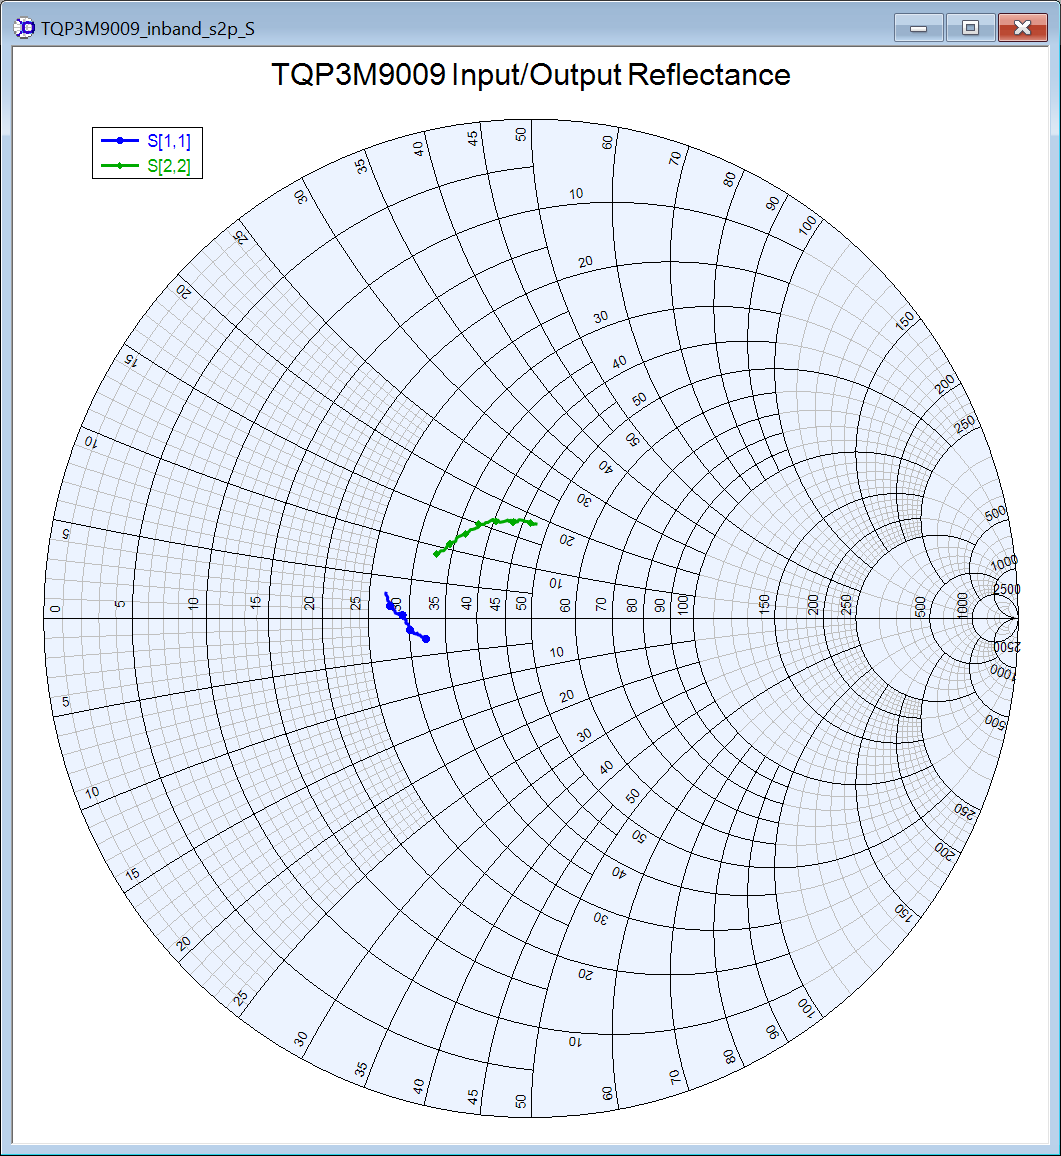
\includegraphics[width=0.44\linewidth]{figs/matching/TQP3M9009_smith}   \label{fig_tqp_smith}
        	}
	\subfigure[RFPA3800 Reflection Coefficients.]{
		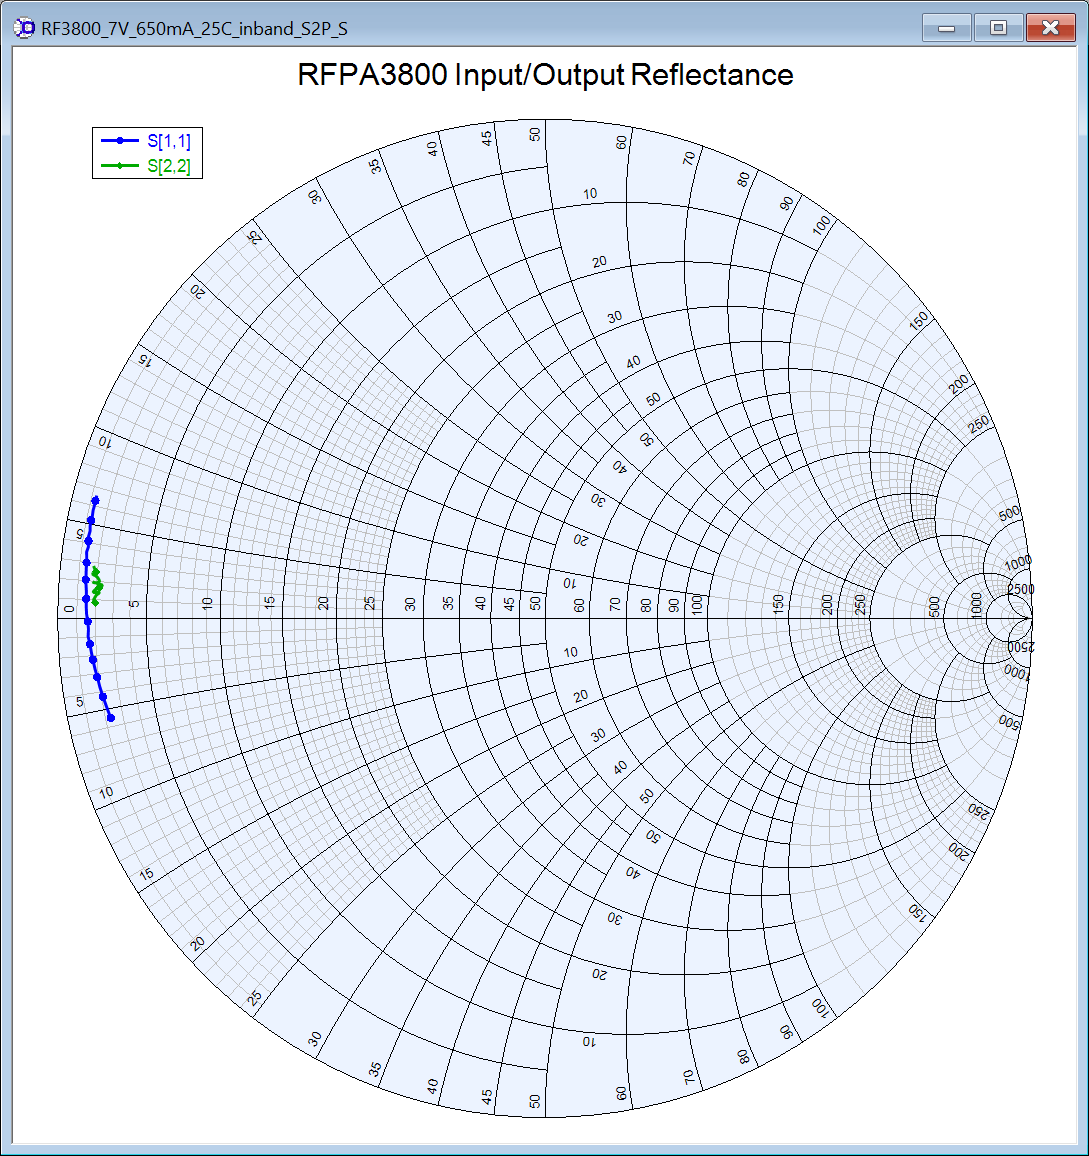
\includegraphics[width=0.45\linewidth]{figs/matching/RFPA3800_smith}   \label{fig_rfpa_smith}
        	}
\caption{Unmatched Smith Chart plots of PA components from 300 - 800 MHz.\label{fig_smith_charts}}
\end{figure*}
	
\subsubsection{Results for TQP3M9009}

	We display the results of the tuned optimization for the TQP3M9009 component in Figure~\ref{fig_srft_tqp}, with the \ac{MAG} (Equation~\ref{eq_mag}) displayed as an upper bound on the achievable matched gain for both the input and output matching circuits.
	In each case, we choose $T_{01} = T_{02} = 25$~dBm as the target flat gain value, represented as the flat dotted green line in Figure~\ref{fig_srft_tqp} (top left, top right).
	These values were chosen by trial and error as the maximum flat gain values that could be supported with this matching circuit.
		The number of matching elements is also chosen through trial and error in order to meet the optimization target with a minimal number of physical components.
		We can tell immediately from the relatively flat T1 and T2 \ac{MAG} that the TQP3M9009 is already well-matched and will require few components to produce a flat gain response.
		This is confirmed by viewing the Smith chart representation \cite{orfanidis2002electromagnetic} of the input and output reflection coefficients of the unmatched amplifier in Figure~\ref{fig_tqp_smith}, where we can see it is already well-matched in a 50~$\Omega$ system. 

	The resulting optimized TQP3M9009 gain with only input matching, $\text{T1}_{\text{dB}}$, and both input and output matching, $\text{T2}_{\text{dB}}$, is shown as solid blue lines.
	Compared to the \ac{MAG}, which represents the optimal gain in the case where each frequency point is optimized individually without regard for a broadband match, our optimized flat passband gain performs quite well.
	
	The physical ideal circuits that realize this optimized gain are also shown in Figure~\ref{fig_srft_tqp} (middle left, middle right).
	Numerical solutions to Equation~\ref{eq_stage_1} result in arbitrary circuit component values, but lumped elements are only available in discrete values.
	Therefore we perform a final processing step to round the solution lumped element component values to their nearest commercially available common values.
	The raw solution and the processed solution based on common component values is given as the second and third rows in Figure~\ref{fig_srft_tqp}.


%\pagebreak


\begin{figure}[p]
\centering
  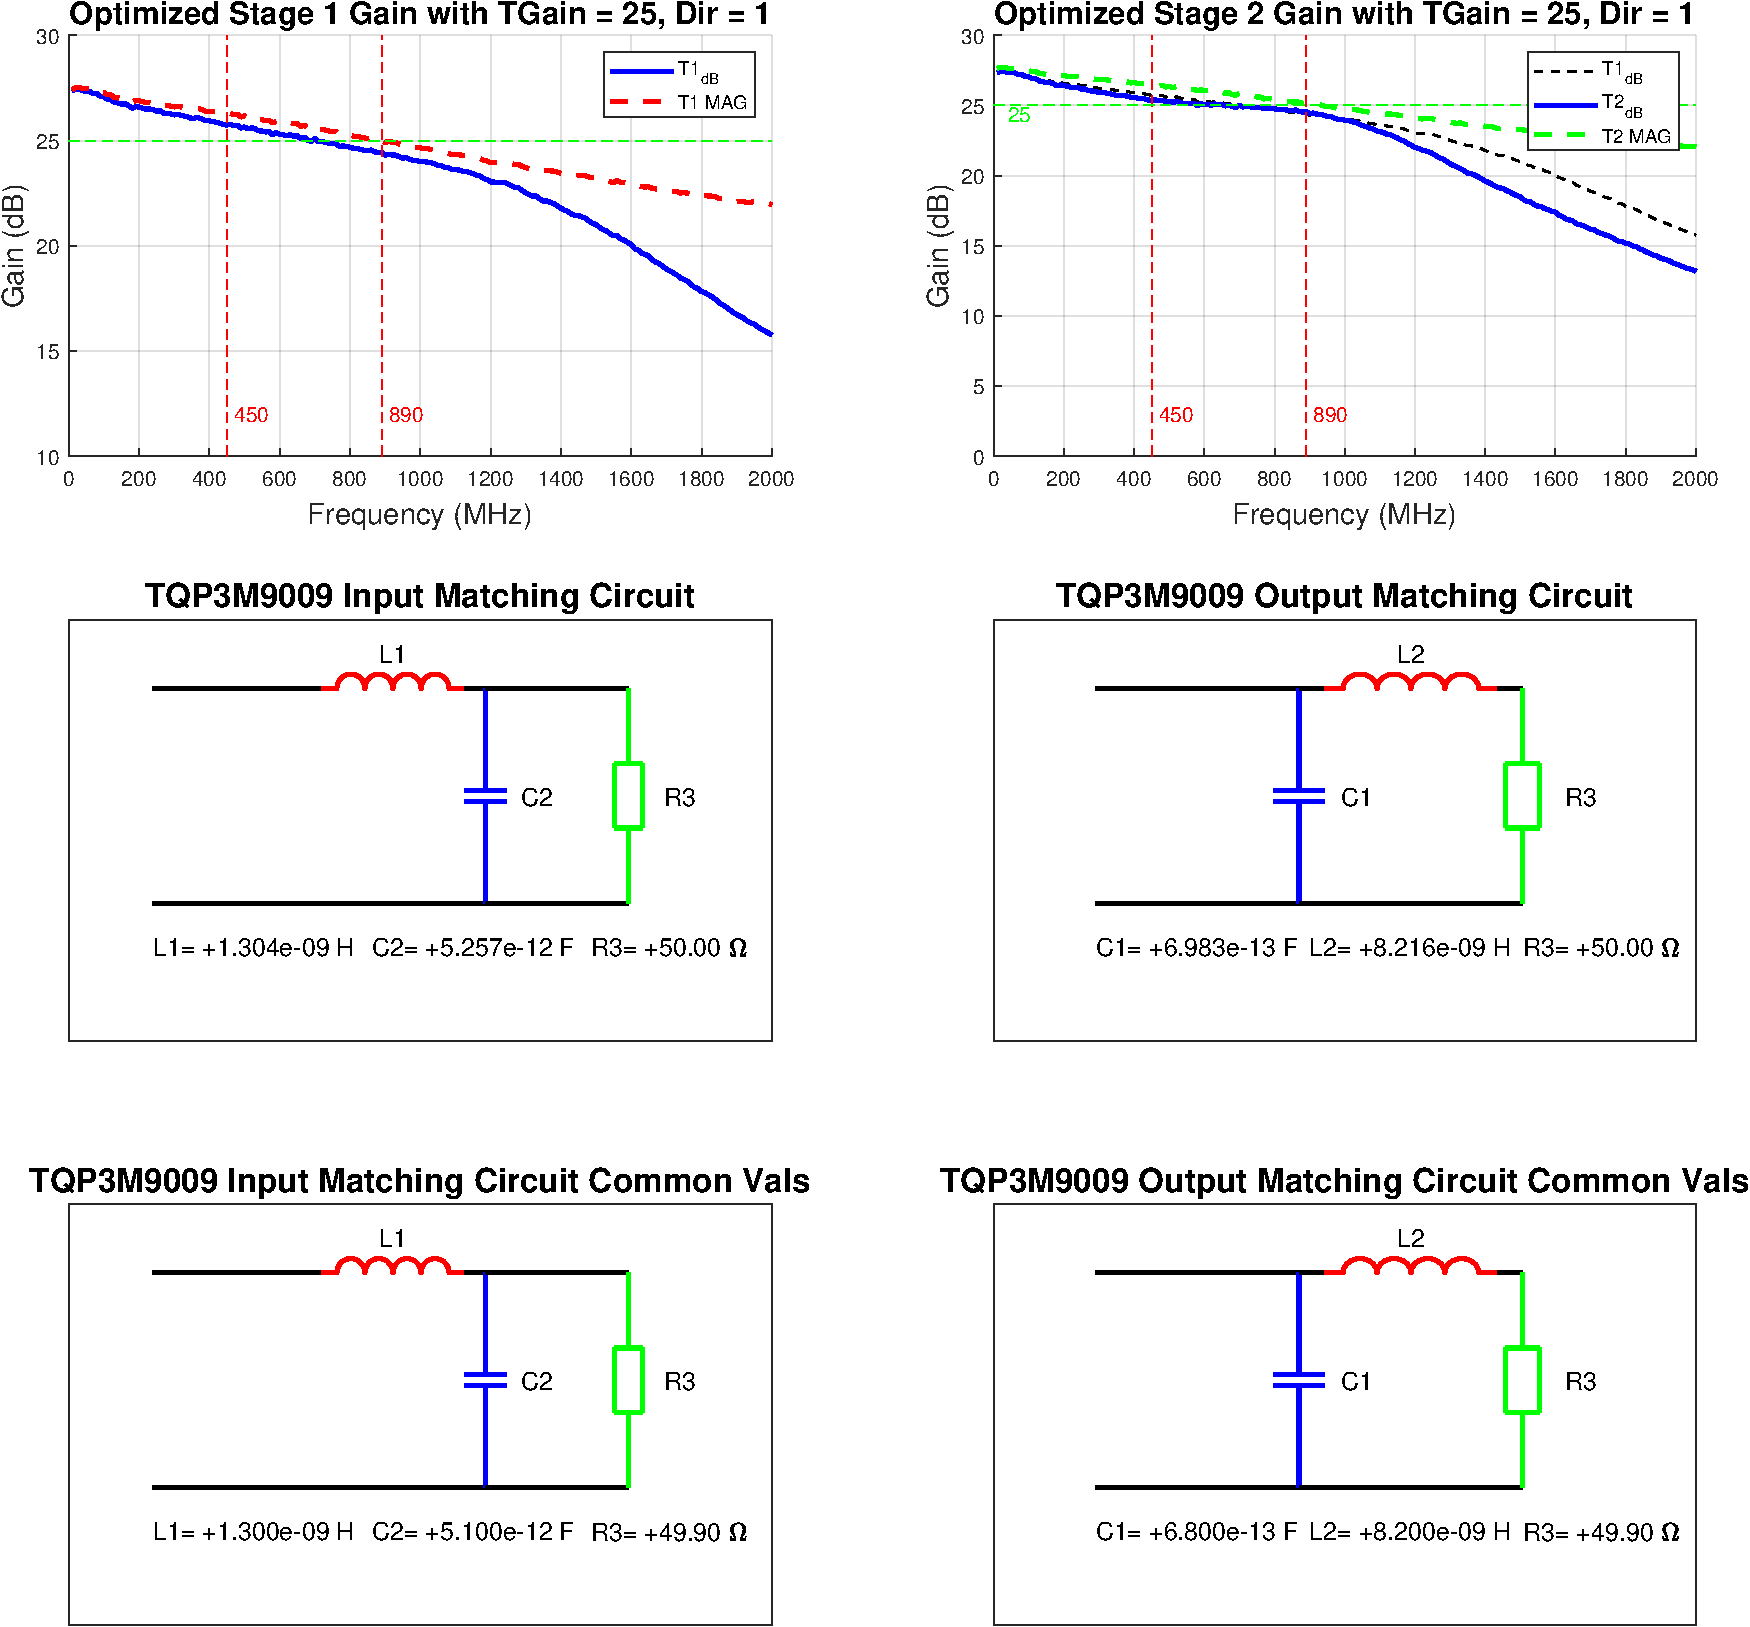
\includegraphics[width=1\linewidth]{figs/matching/14-Oct-2018_TQP3M9009_srft_results_sequential}   
    \caption{50-$\Omega$ input and output broadband match and synthesized circuit for 1st stage TQP3M9009 amplifier.}
\label{fig_srft_tqp}
\end{figure}


\pagebreak


%
%
%\begin{equation}
	%\argmax_{\textbf{[E]}}{T(\omega)} = |G_{21}|^2\frac{|E_{21}|^2}{|1-E_{11}G_{22}|^2|1-\hat{E}_{22}L_{11}|^2}|L_{21}|^2
%\end{equation}

\subsubsection{Results for RFPA3800}

	We display the results of the same tuned optimization for the RFPA3800 component in Figure~\ref{fig_srft_rfpa}, with the \ac{MAG} (Equation~\ref{eq_mag}) displayed as an upper bound on the achievable matched gain for both the input and output matching circuits.
	
	In this case, we empirically choose $T_{03} = 7.8$ and $T_{04} = 15.3$~dBm as the target flat gain value, represented as the flat dotted green line in Figure~\ref{fig_srft_rfpa} (top left, top right).
		
	The RFPA3800 presents a more difficult circuit to match; from its unmatched Smith Chart representation in Figure~\ref{fig_rfpa_smith} it is not internally matched to a 50~$\Omega$ system.
	This is a common occurrence with most high-power amplifiers or transistors, which leaves flexibility to the microwave designer, but also means we will need to apply more effort to get the part matched to 50~$\Omega$.

	This means that there is a larger different between the RFPA3800 T3 and T4 \ac{MAG} and its optimized flat gain, as shown in Figure~\ref{fig_srft_rfpa} (top left, top right).
	For the same reason, a larger number of matching components are required to achieve a reasonable flat frequency response across the band from 470 - 700~MHz and a few dB of gain compared to the upper bound \ac{MAG} are sacrificed in order to achieve this relatively flat gain target.
	
	We extended the upper frequency range in our final optimization of this broadband matching circuit to 800~MHz based on our experience implementing the circuit and finding that high-band performance above 650~MHz suffered from parasitics.
	This extra effort extends the lowpass roll off of the power transfer circuit topology higher to ensure that performance below 700~MHz remains nominal once implemented as a physical circuit.

\begin{figure}[p]
\centering
  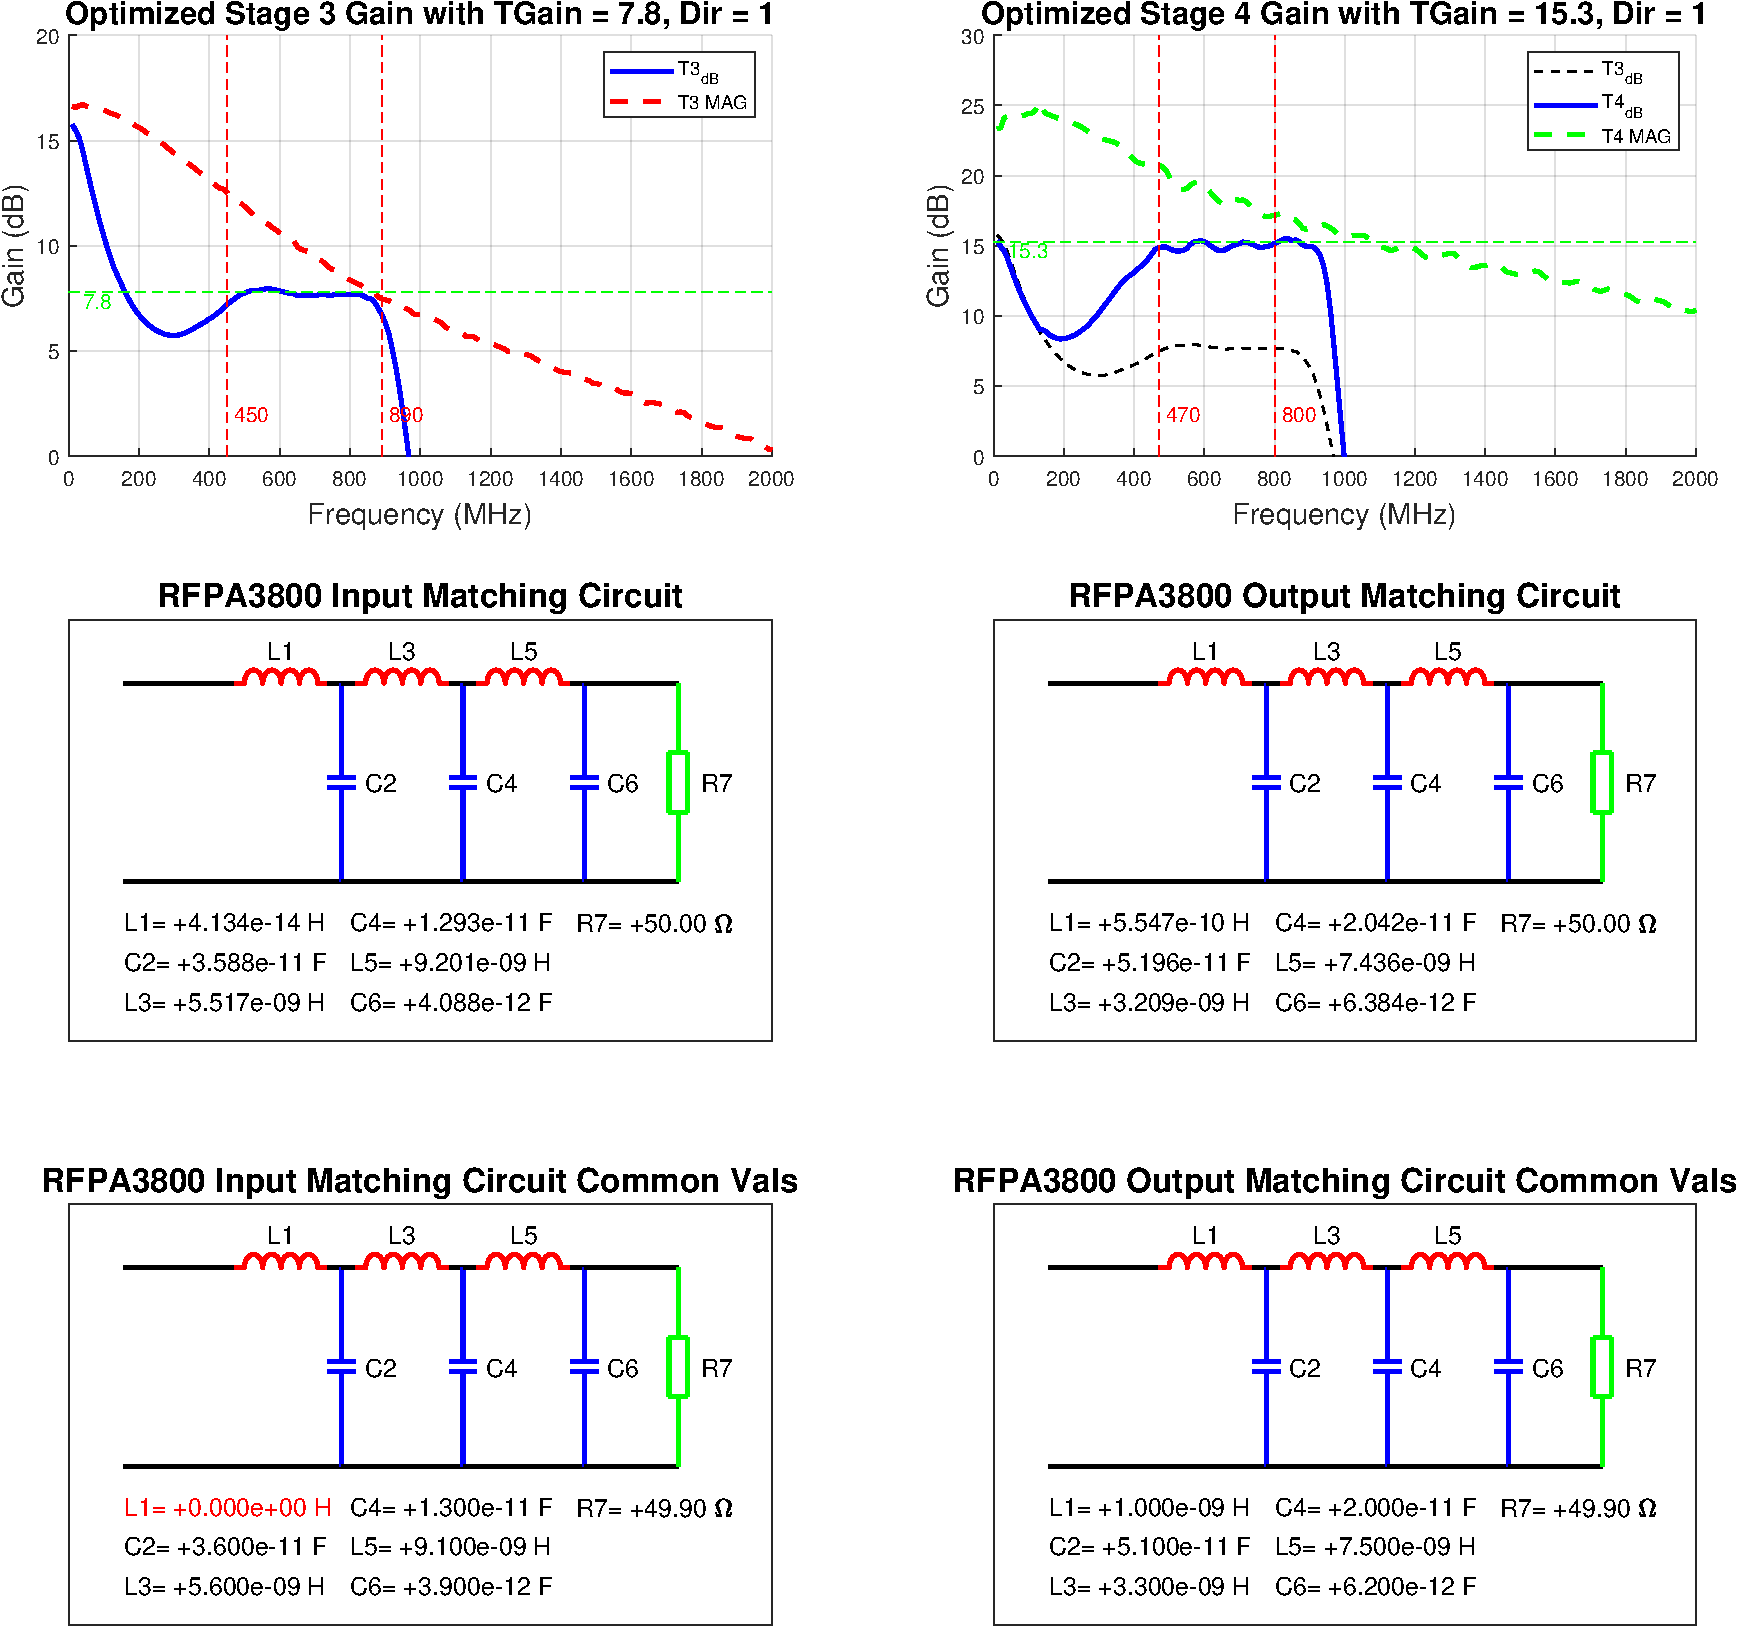
\includegraphics[width=1\linewidth]{figs/matching/14-Oct-2018_RFPA3800_srft_results_sequential}   
    \caption{50-$\Omega$ input and output broadband match and synthesized circuit for 2nd stage RFPA3800 amplifier.}
\label{fig_srft_rfpa}
\end{figure}


\pagebreak


%\begin{figure}[h]
%\centering
  %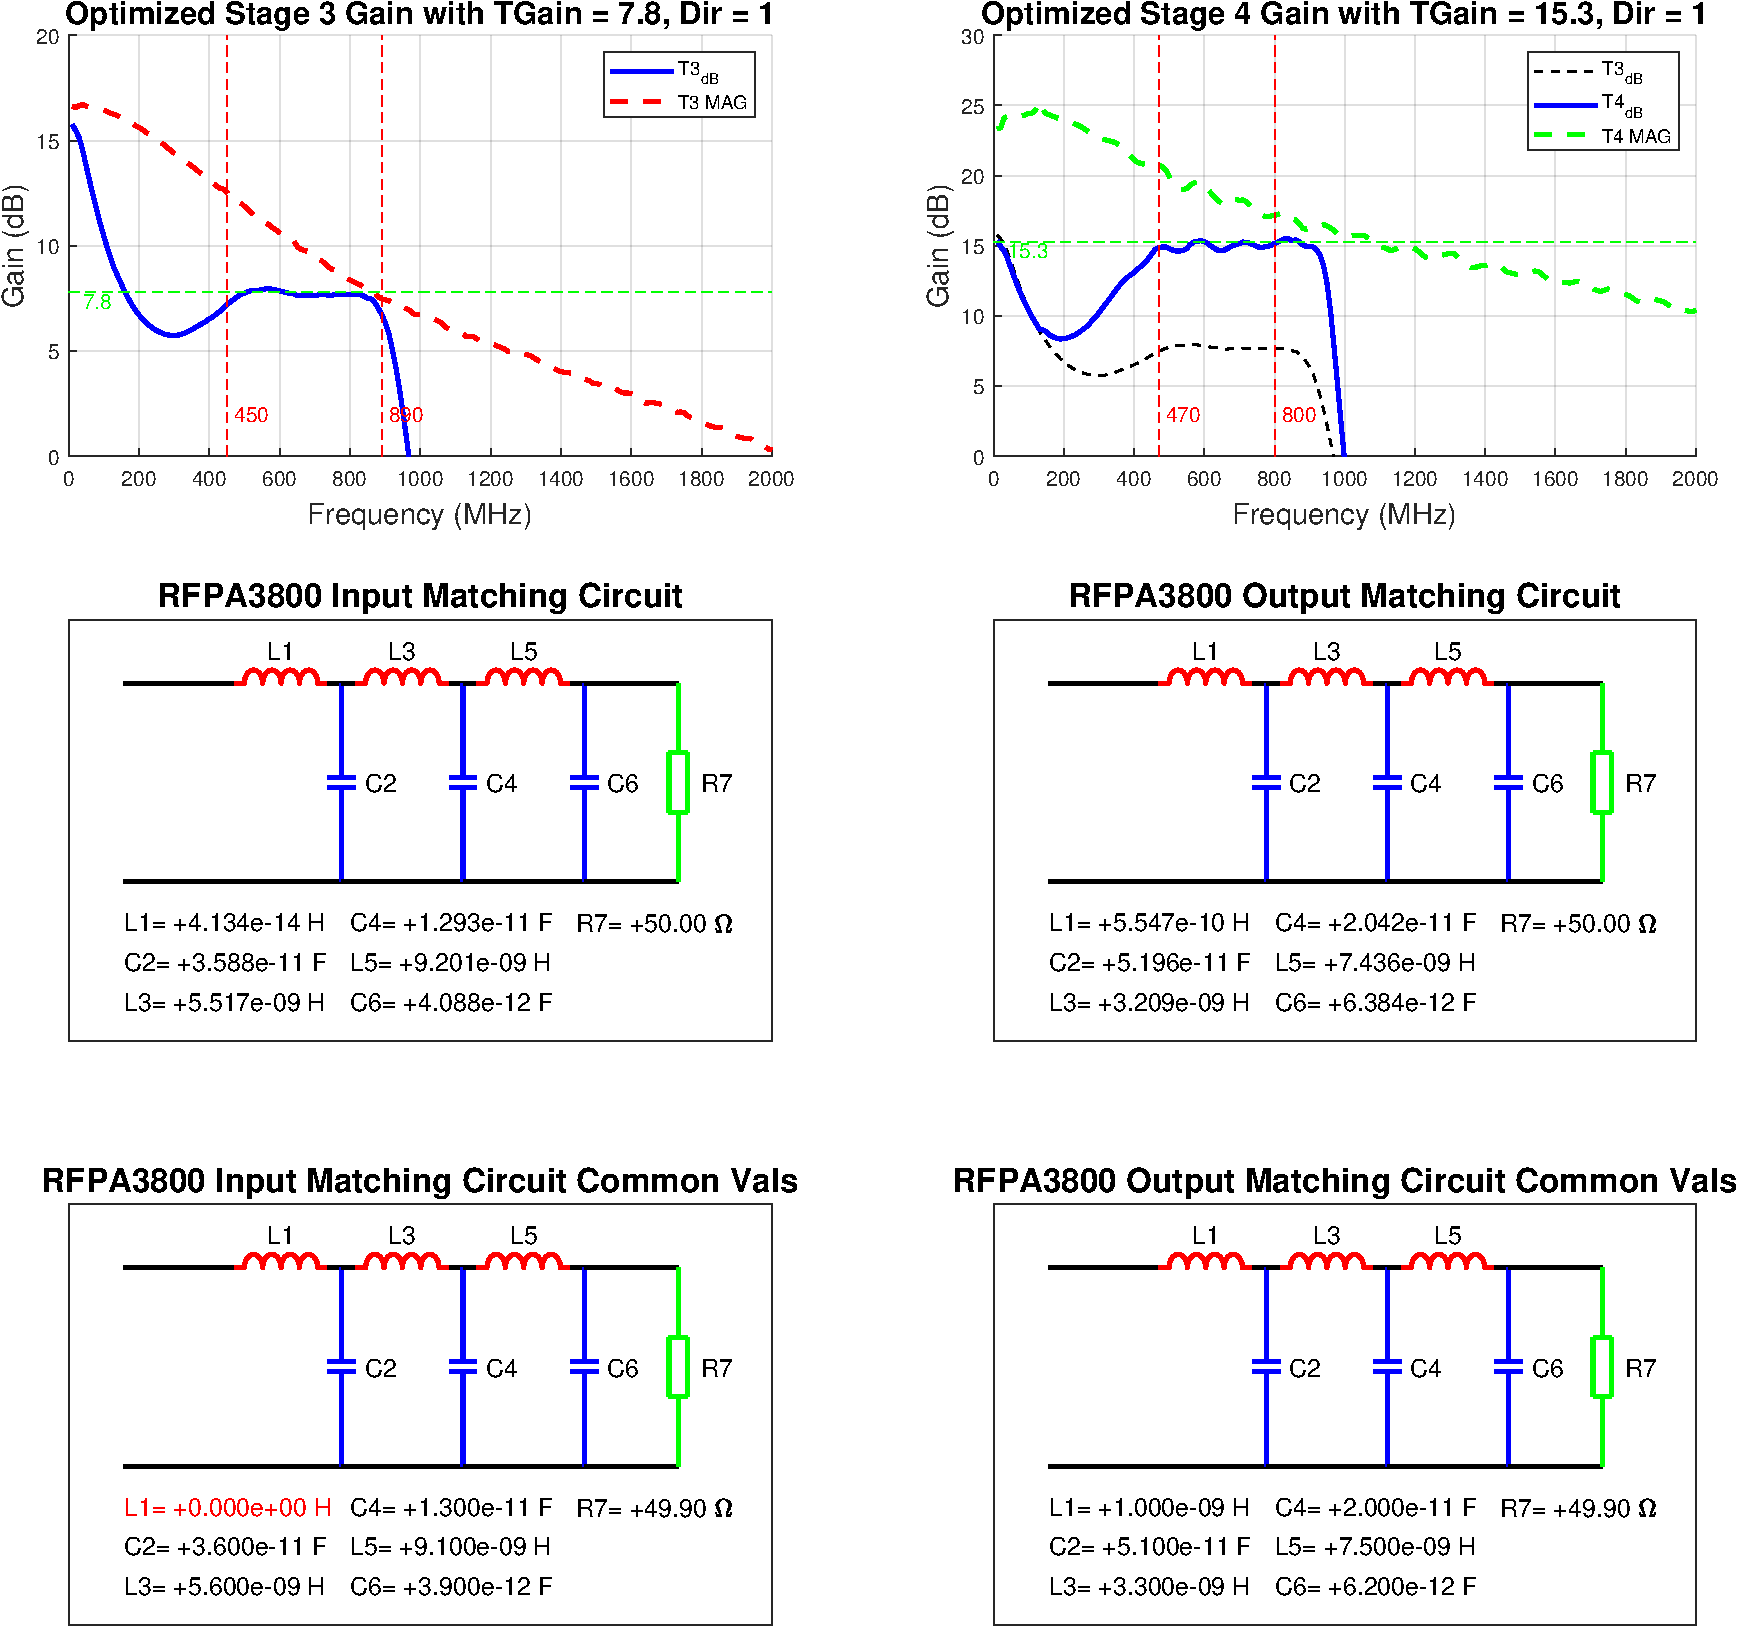
\includegraphics[width=0.9\linewidth]{figs/matching/14-Oct-2018_RFPA3800_srft_results_sequential} 
    %\caption{50-$\Omega$ input and output broadband match and synthesized circuit for RFPA3800 amplifier.}
%\label{fig_srft_rfpa}
%\end{figure}


%##################################################
\subsection{Simulation of Broadband Matching Networks}
\label{sec_broadband_ideal}
% XSPICE simulation circuit and results

%\begin{figure}[h]
%\centering
  %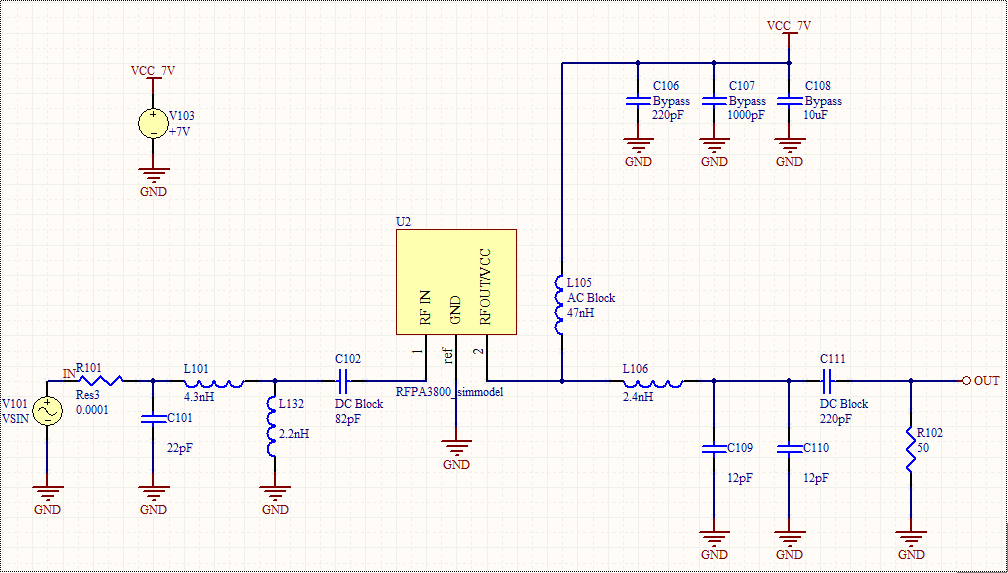
\includegraphics[width=4in]{figs/matching/RFPA3800_circuit}   
    %\caption{SPICE simulation circuit for ideal broadband power transfer network}
%\label{fig:tx_power_plot}
%\end{figure}

	In this section, we present an early prototype of the \ac{WURC} broadband power transfer network that utilized the same real frequency numerical optimization design technique as discussed in Section~\ref{sec_srft_stage_1} and \ref{sec_srft_stage_2}, but rather than matching each amplifier to a 50~$\Omega$ input and output impedance, the multiple stages were cascaded into each other following the general procedure outlined in Yarman 1982 \cite{yarman1982simplified}.
	The intent of these simulations were to confirm the validity of the designed broadband matching circuit before producing physical prototypes; however we found that both our design technique as well as our modeling approach was insufficient to fully represent the physical realization of the broadband matching circuit.
	In this section we will discuss in detail why this occurred and the additional steps needed to implement the ideal broadband power transfer network developed in Section~\ref{sec_dual_match}.

	The initial prototype circuit design is shown in Figure~\ref{fig_spice_circuit}, where XSPICE models for the amplifier elements were extracted from the empirical S-parameter files using EMtoSPICE \cite{mandrutareduced}, a commercial tool for extracting stable time-domain simulation models from frequency-domain S-parameter data.
	We used the built-in XSPICE simulator in \ac{CAD} tool Altium Designer 13 to simulate the steady-state frequency response of the broadband amplifier chain.
	In Figure~\ref{fig_spice_results}, we show the broadband matching gain as a function of the center frequency.
	Both a match to a 65~$\Omega$ (blue) and 50~$\Omega$ (red) differential source impedance were simulated, as we had not yet decided how to compensate for the LMS6002D's 65~$\Omega$ source impedance.
	
	With a minimum simulated 39.2~dBm in-band gain matched against a 50~$\Omega$ source, this was sufficiently close to the designed frequency response that a prototype \ac{PCB} was fabricated to implement the circuit for testing and fine-tuning.
	
% SPICE Model Circuit
\begin{figure}[p]
\centering
  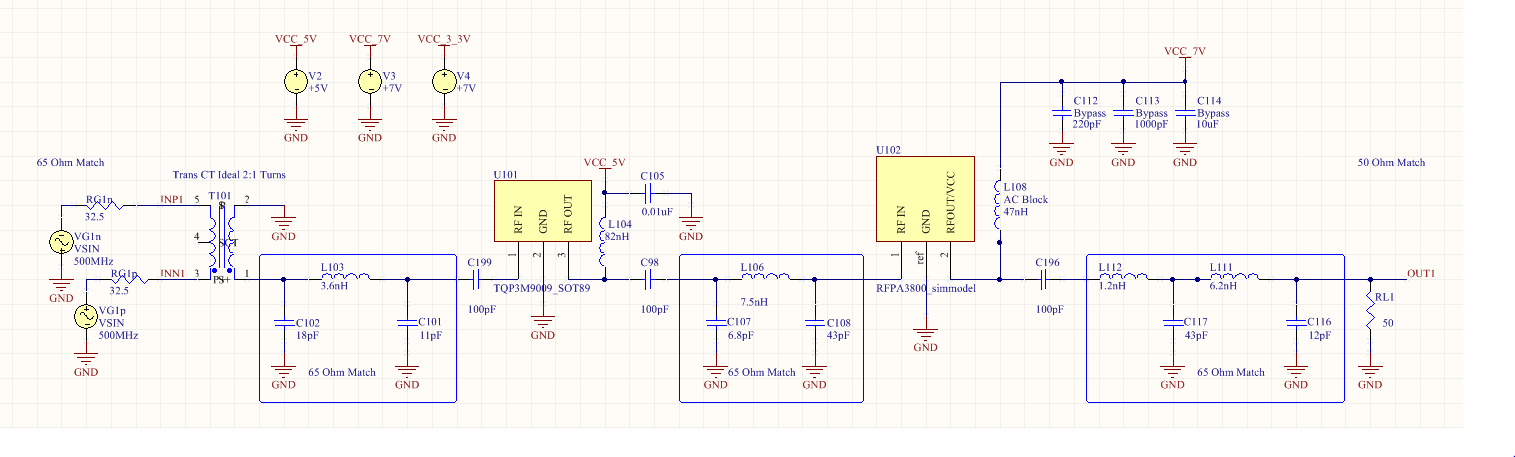
\includegraphics[width=1\linewidth]{figs/matching/tqp_rfpa_circuit_50_65_load}   
    \caption{XSPICE simulation circuit for ideal broadband power transfer network.}
\label{fig_spice_circuit}
\end{figure}

% SPICE Simulation Results
\begin{figure}[p]
\centering
  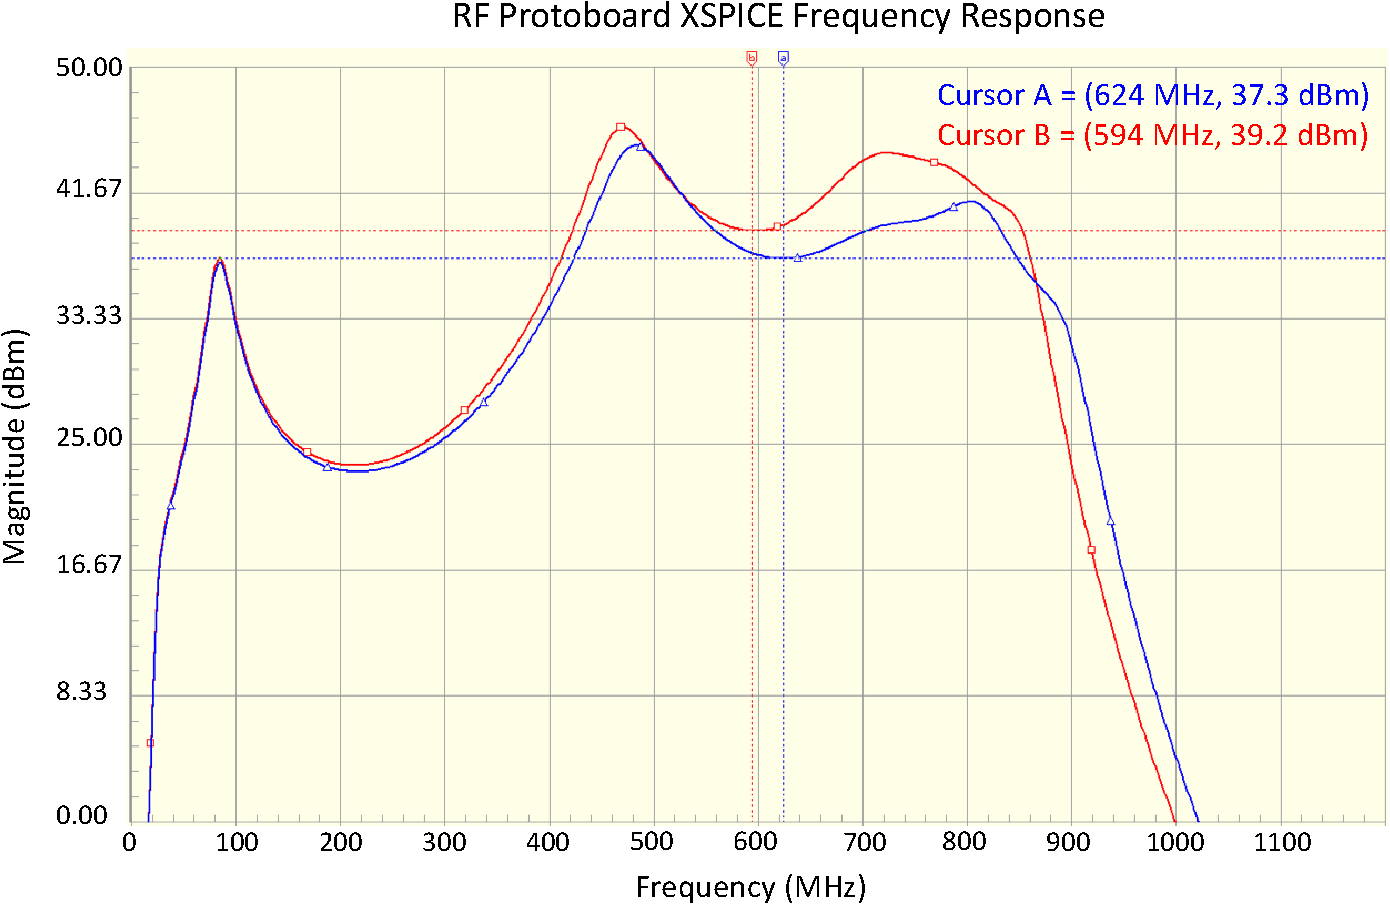
\includegraphics[width=0.9\linewidth]{figs/matching/RF_Protoboard_XSPICE}   
    \caption{XSPICE simulation results of ideal broadband power transfer network.}
\label{fig_spice_results}
\end{figure} 
	
% #########
\subsubsection{Evaluation of Broadband Matching Networks}
\label{sec_rf_protoboard}
% RF Protoboard and results
	
	We designed and manufactured a controlled impedance 2-layer PCB to implement the circuit presented in Figure~\ref{fig_spice_circuit} \ref{sec_broadband_ideal}.
	With 50~$\Omega$ input and output, the circuit was designed to provide space for any additional matching components and RF probes.
	%An additional pass-through 50~$\Omega$ microstrip trace was provided to de-embed the PCB or individual components, should that become necessary.
	The assembled PCB is shown in Figure~\ref{fig_match_proto_pcb}.
	The extra grounding copper foil shown in the picture was added after initial characterization and can be ignored.
	
	The prototype amplification PCB was measured with a calibrated vector network analyzer and it became clear that the physical device performance was not matching simulated results.
	We show the actual $|S_{21}|$, or forward gain, of the cascaded designed gain stages in Figure~\ref{fig_match_proto_gain}, where we can immediately see that gain unexpectedly drops off to zero drastically after approximately 500~MHz whereas the designed circuit maintained a flat gain out beyond 800~MHz in simulation.

% RF Prototype Board for UHF RF PAs
\begin{figure}[p]
\centering
  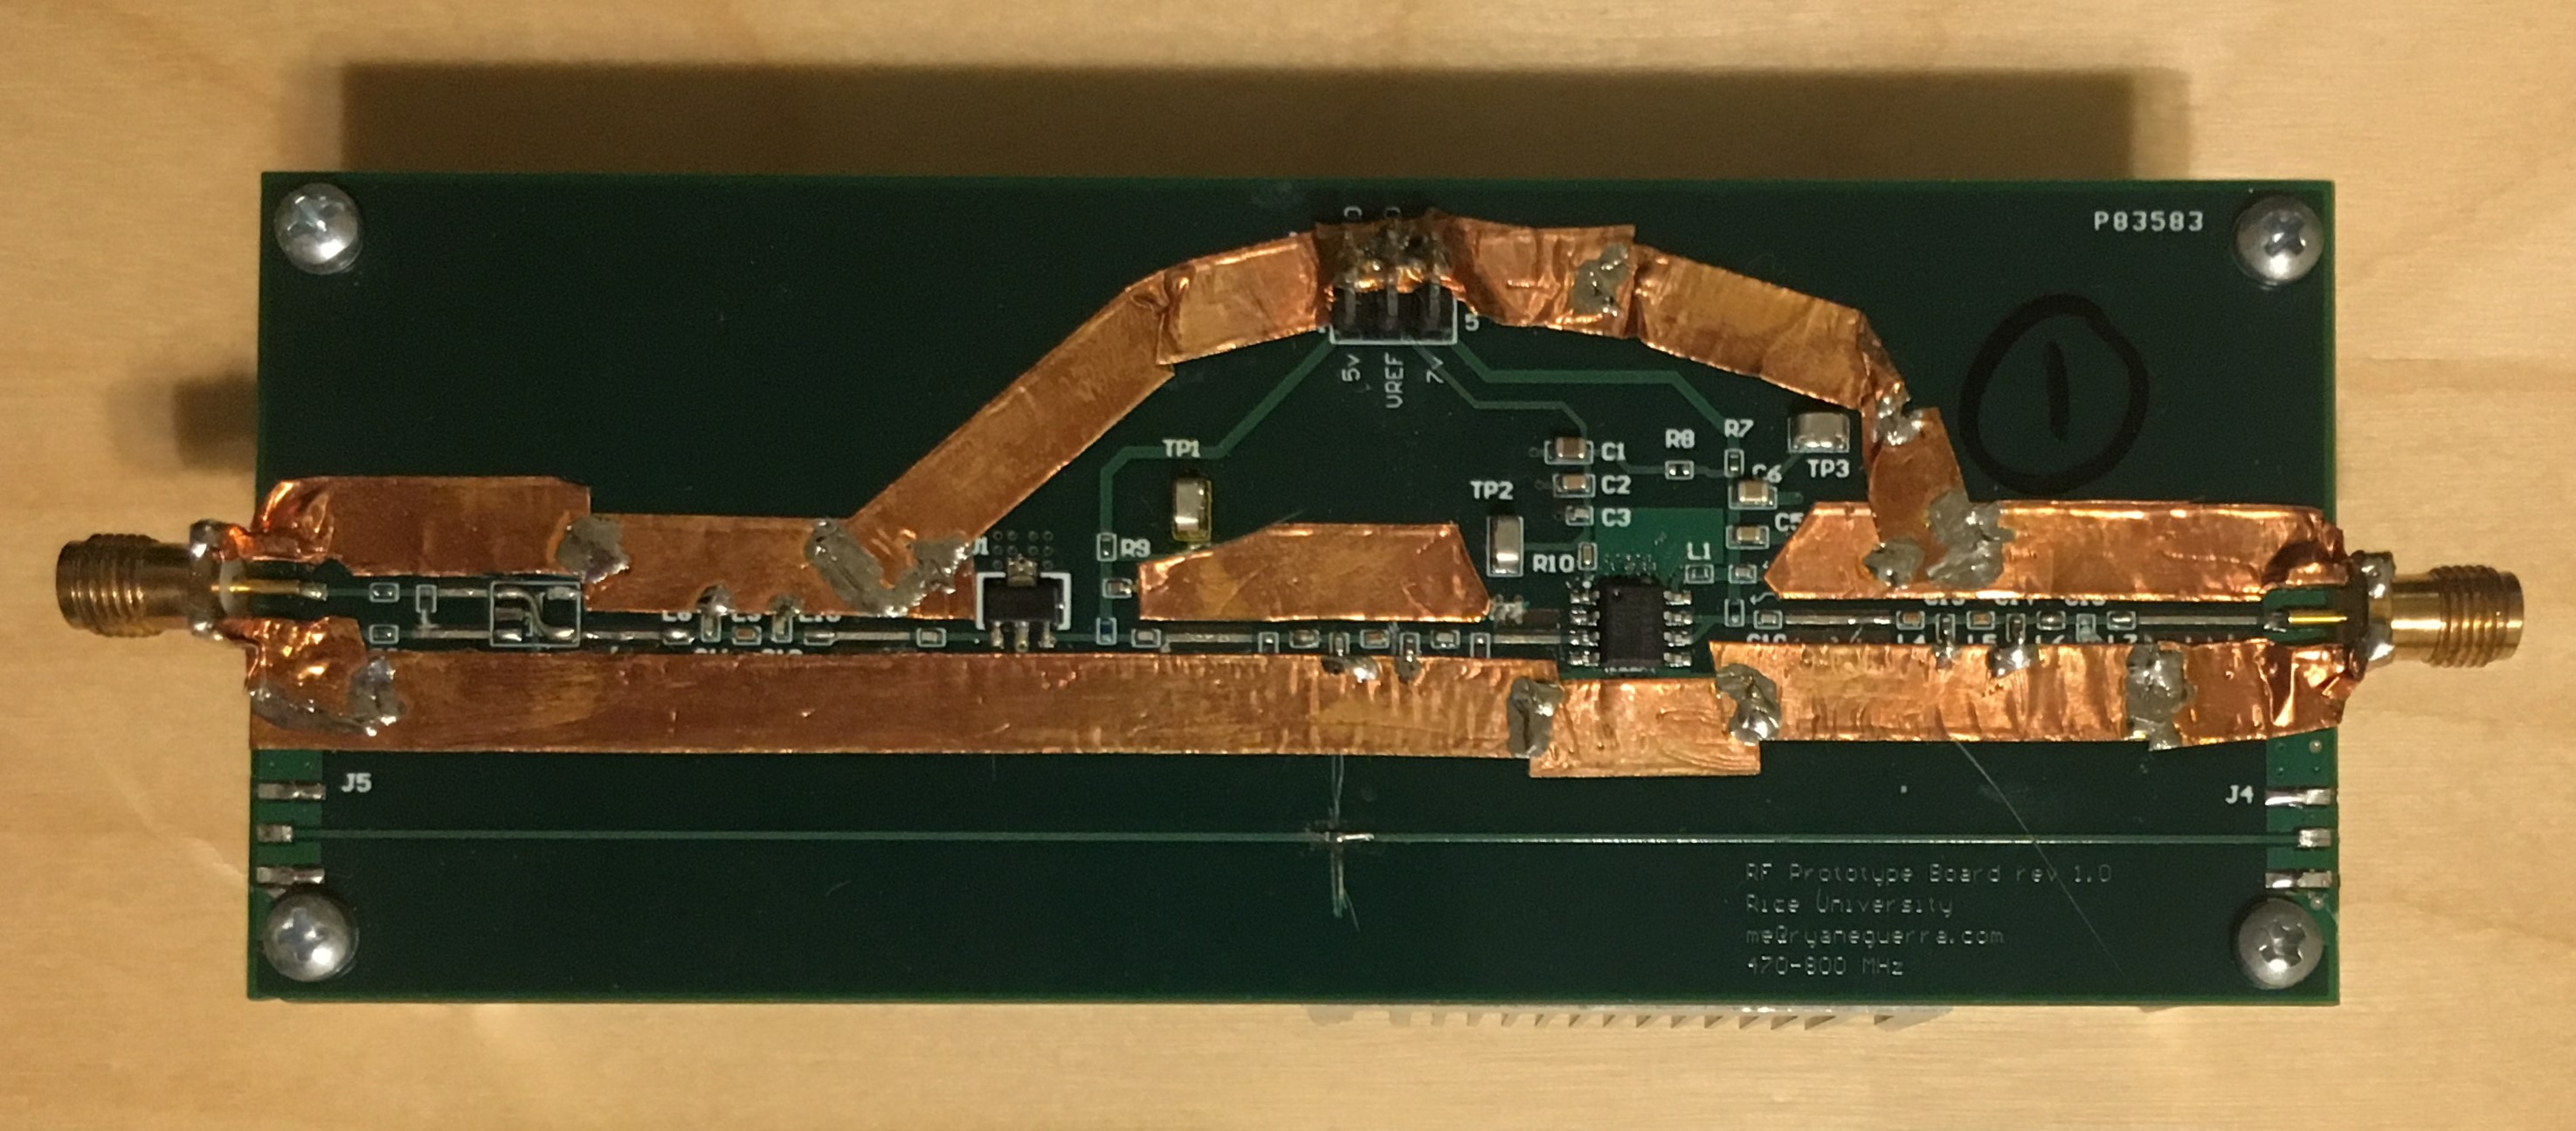
\includegraphics[width=1\linewidth]{figs/matching/rf_protoboard}   
    \caption{Prototype PCB of WURC broadband power transfer circuit.}
\label{fig_match_proto_pcb}
\end{figure}

% Gain Plot for RF Prototype Board
\begin{figure}[p]
\centering
  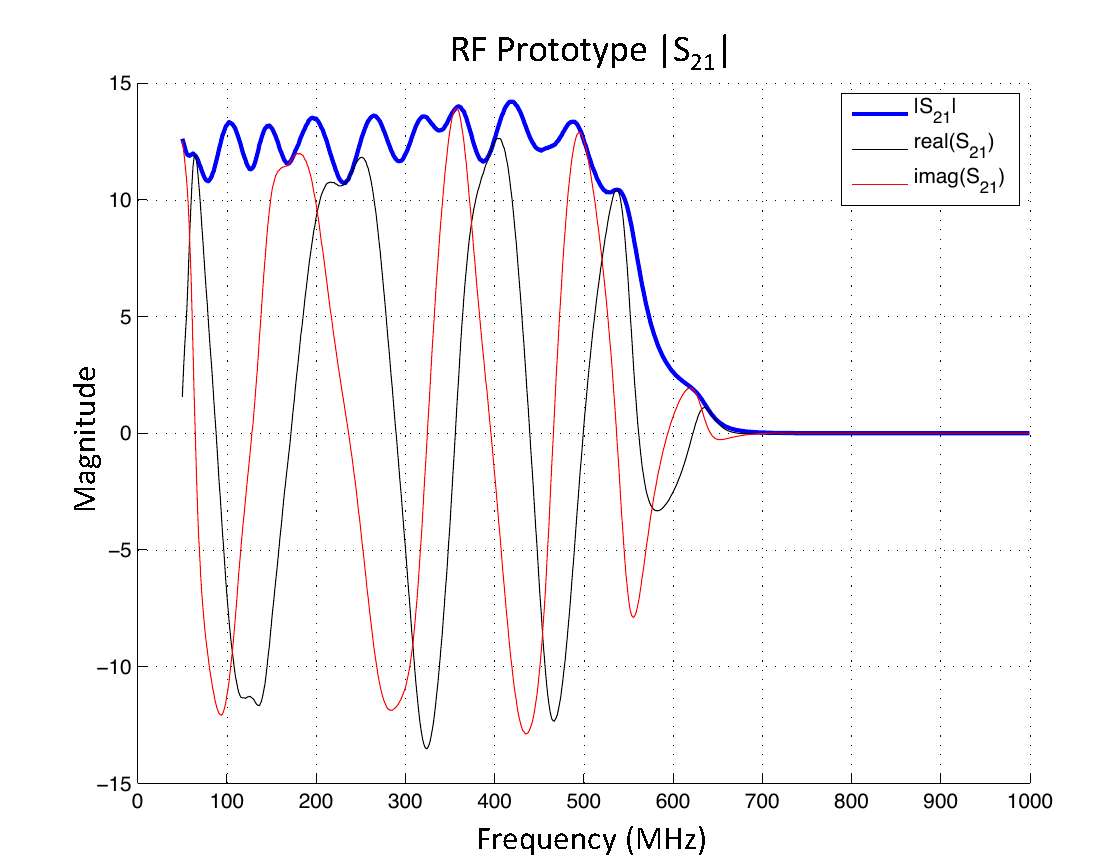
\includegraphics[width=0.8\linewidth]{figs/matching/RF_Protoboard_S21_measured}   
    \caption{Measured gain of prototype WURC broadband power transfer circuit.}
\label{fig_match_proto_gain}
\end{figure}


	The root cause of this unintended result is the inability of the real-frequency matching technique to directly consider parasitic circuit elements in its formulation.
	It is a well-characterized fact that physical circuit elements are non-ideal: coupling between physical elements and construction from non-ideal materials yields parasitic resistance, capacitance, and inductance in each lumped-element component.
	A chip capacitor in particular has a \ac{SRF}, $\omega_0 = \frac{1}{\sqrt{L_p\cdot C}}$, when the desired series capacitance resonates with the parasitic series inductance of the part \cite{murata2010srf}.
	Below the resonant frequency, the capacitance term dominates; above the resonant frequency, the parasitic inductive term dominates and the physical capacitor no longer behaves like an ideal capacitor.
	
	\pagebreak
	
	For example, we present the empirical impedance functions provided by the component manufacturer of three chip capacitors considered in our matching circuit design in Figure~\ref{fig_cap_comparison}: a 16~pF 0201 (GRM0335C1H160 blue), a 5~pF 0402 (GJM1555C1H5R0 green), and a 47~pF 0402 (GJM1555C1H470 red).
	These capacitors were considered to implement the circuit in Figure~\ref{fig_spice_results}, specifically component C117 in that diagram.
	
	The 47~pF 0402 component has a self-resonant frequency of approximately 1600~MHz, represented by the trough in the red curve in Figure~\ref{fig_cap_comparison}.
	As a rule of thumb, the \ac{SRF} of a component should be selected to be approximately 3-times larger than the maximum operating frequency of the circuit for filters and matching application in order to ensure that its behavior approaches its expected ideal behavior.
	We confirmed that this particular capacitor was behaving in a non-ideal manner due to its low \ac{SRF} that effectively destroyed the designed conjugate match above 500~MHz in the implemented circuit.
	
	In general, larger value capacitances and larger physical packages result in lower \ac{SRF}, so we focused on reducing both parameters.
	
% Self-resonant frequencies for capacitors in WURC
\begin{figure}[hb]
\centering
  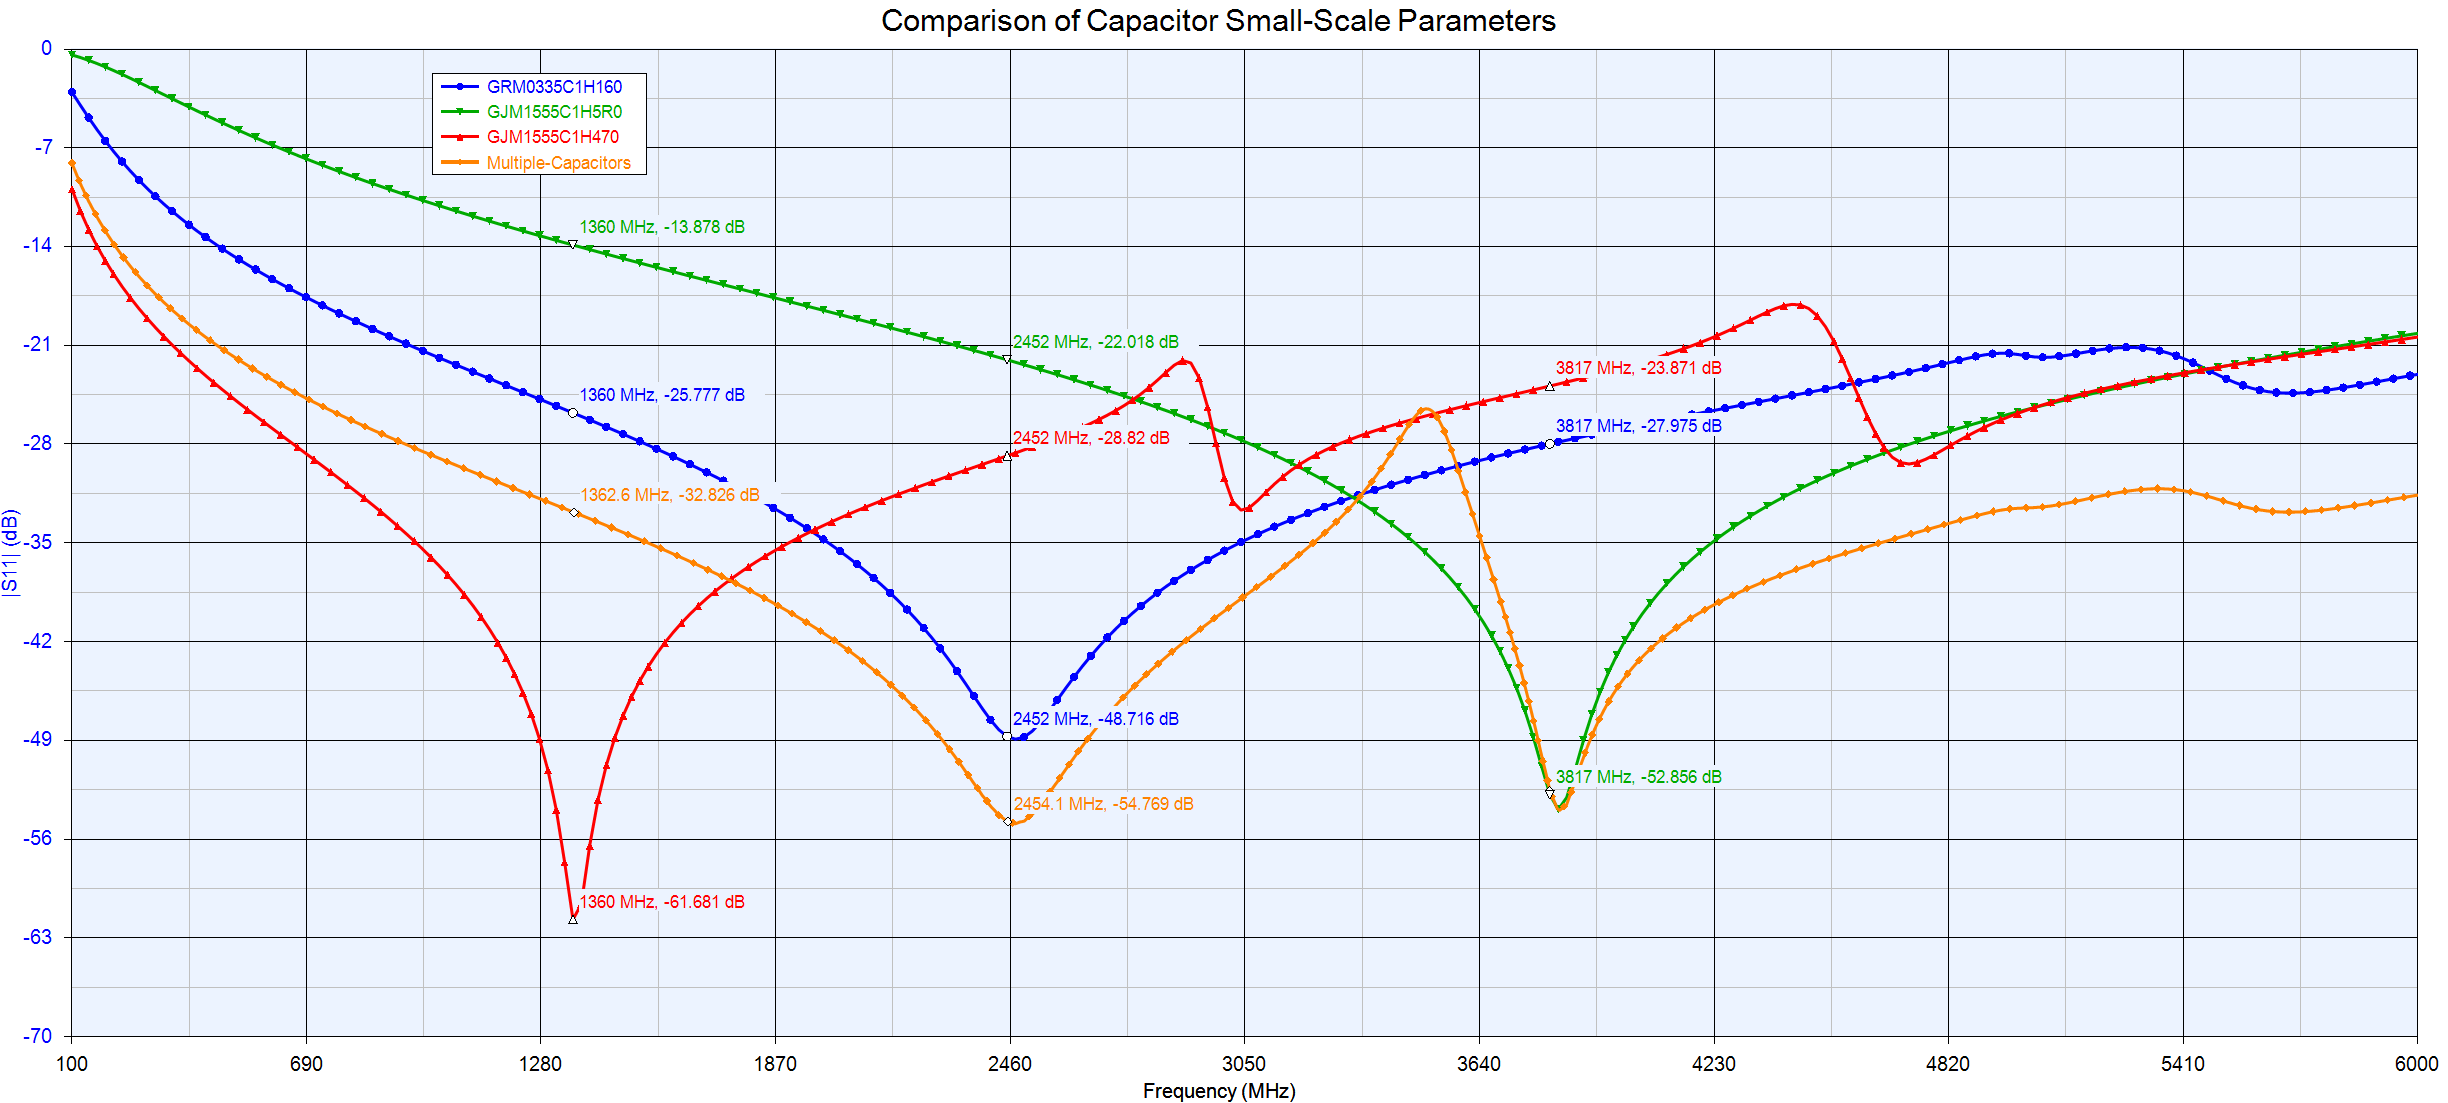
\includegraphics[width=1\linewidth]{figs/matching/capacitor_comparison}   
    \caption{S-parameters for various MLCC capacitor configurations.}
\label{fig_cap_comparison}
\end{figure}
	
	After much iteration with small-scale simulation techniques that could accurately model the parasitics, we decided to replace the 47~pF 0402 with three different capacitors in parallel: two 16~pF 0201 and one 5~pF 0402 capacitor.
	The \ac{SRF} for these two parts was respectively 2450~MHz and 3820~MHz, well above the maximum 800~MHz operating range of the amplifiers; the combined frequency response of this parallel circuit is shown in Figure~\ref{fig_cap_comparison} as the orange plotline.
		

%##################################################
\subsection{Simulation of Broadband Matching Networks with Parasitics}
\label{sec_wurc_parasitics}

	While this design was confirmed at the early design stage with XSPICE simulation models, evaluation of the prototypes presented earlier demonstrated that package parasitics in the lumped-element broadband power transfer chain were missing from the XSPICE simulator models.
	These parasitics severely impaired the implemented high-frequency gain response above 500~MHz and required a more advanced model and simulation technique to correctly predict their effect.
	Re-modeling the RF chain in the Cadence Virtuoso SpectreRF circuit simulator utilizing empirical S-parameter models resulted in a more accurate simulation, allowing package parasitics to be compensated for in the lumped-element design.

	We considered the entire physical layout in SpectreRF, including transformers, microstrip, switches and filters.
	For each discrete component, empirical S-parameter files were obtained from the equipment manufacturer or directly generated from development boards using a vector network analyzer.
	The resulting physical model considering parasitics and layout is shown in Figure~\ref{fig_spectre_uhf_circuit} for the entire \ac{WURC} UHF transmit chain.
	
% PAGEBREAK  vvvvvvvvvvvvvv
% SpectreRF full RF chain model
\begin{figure}[p]
\centering
  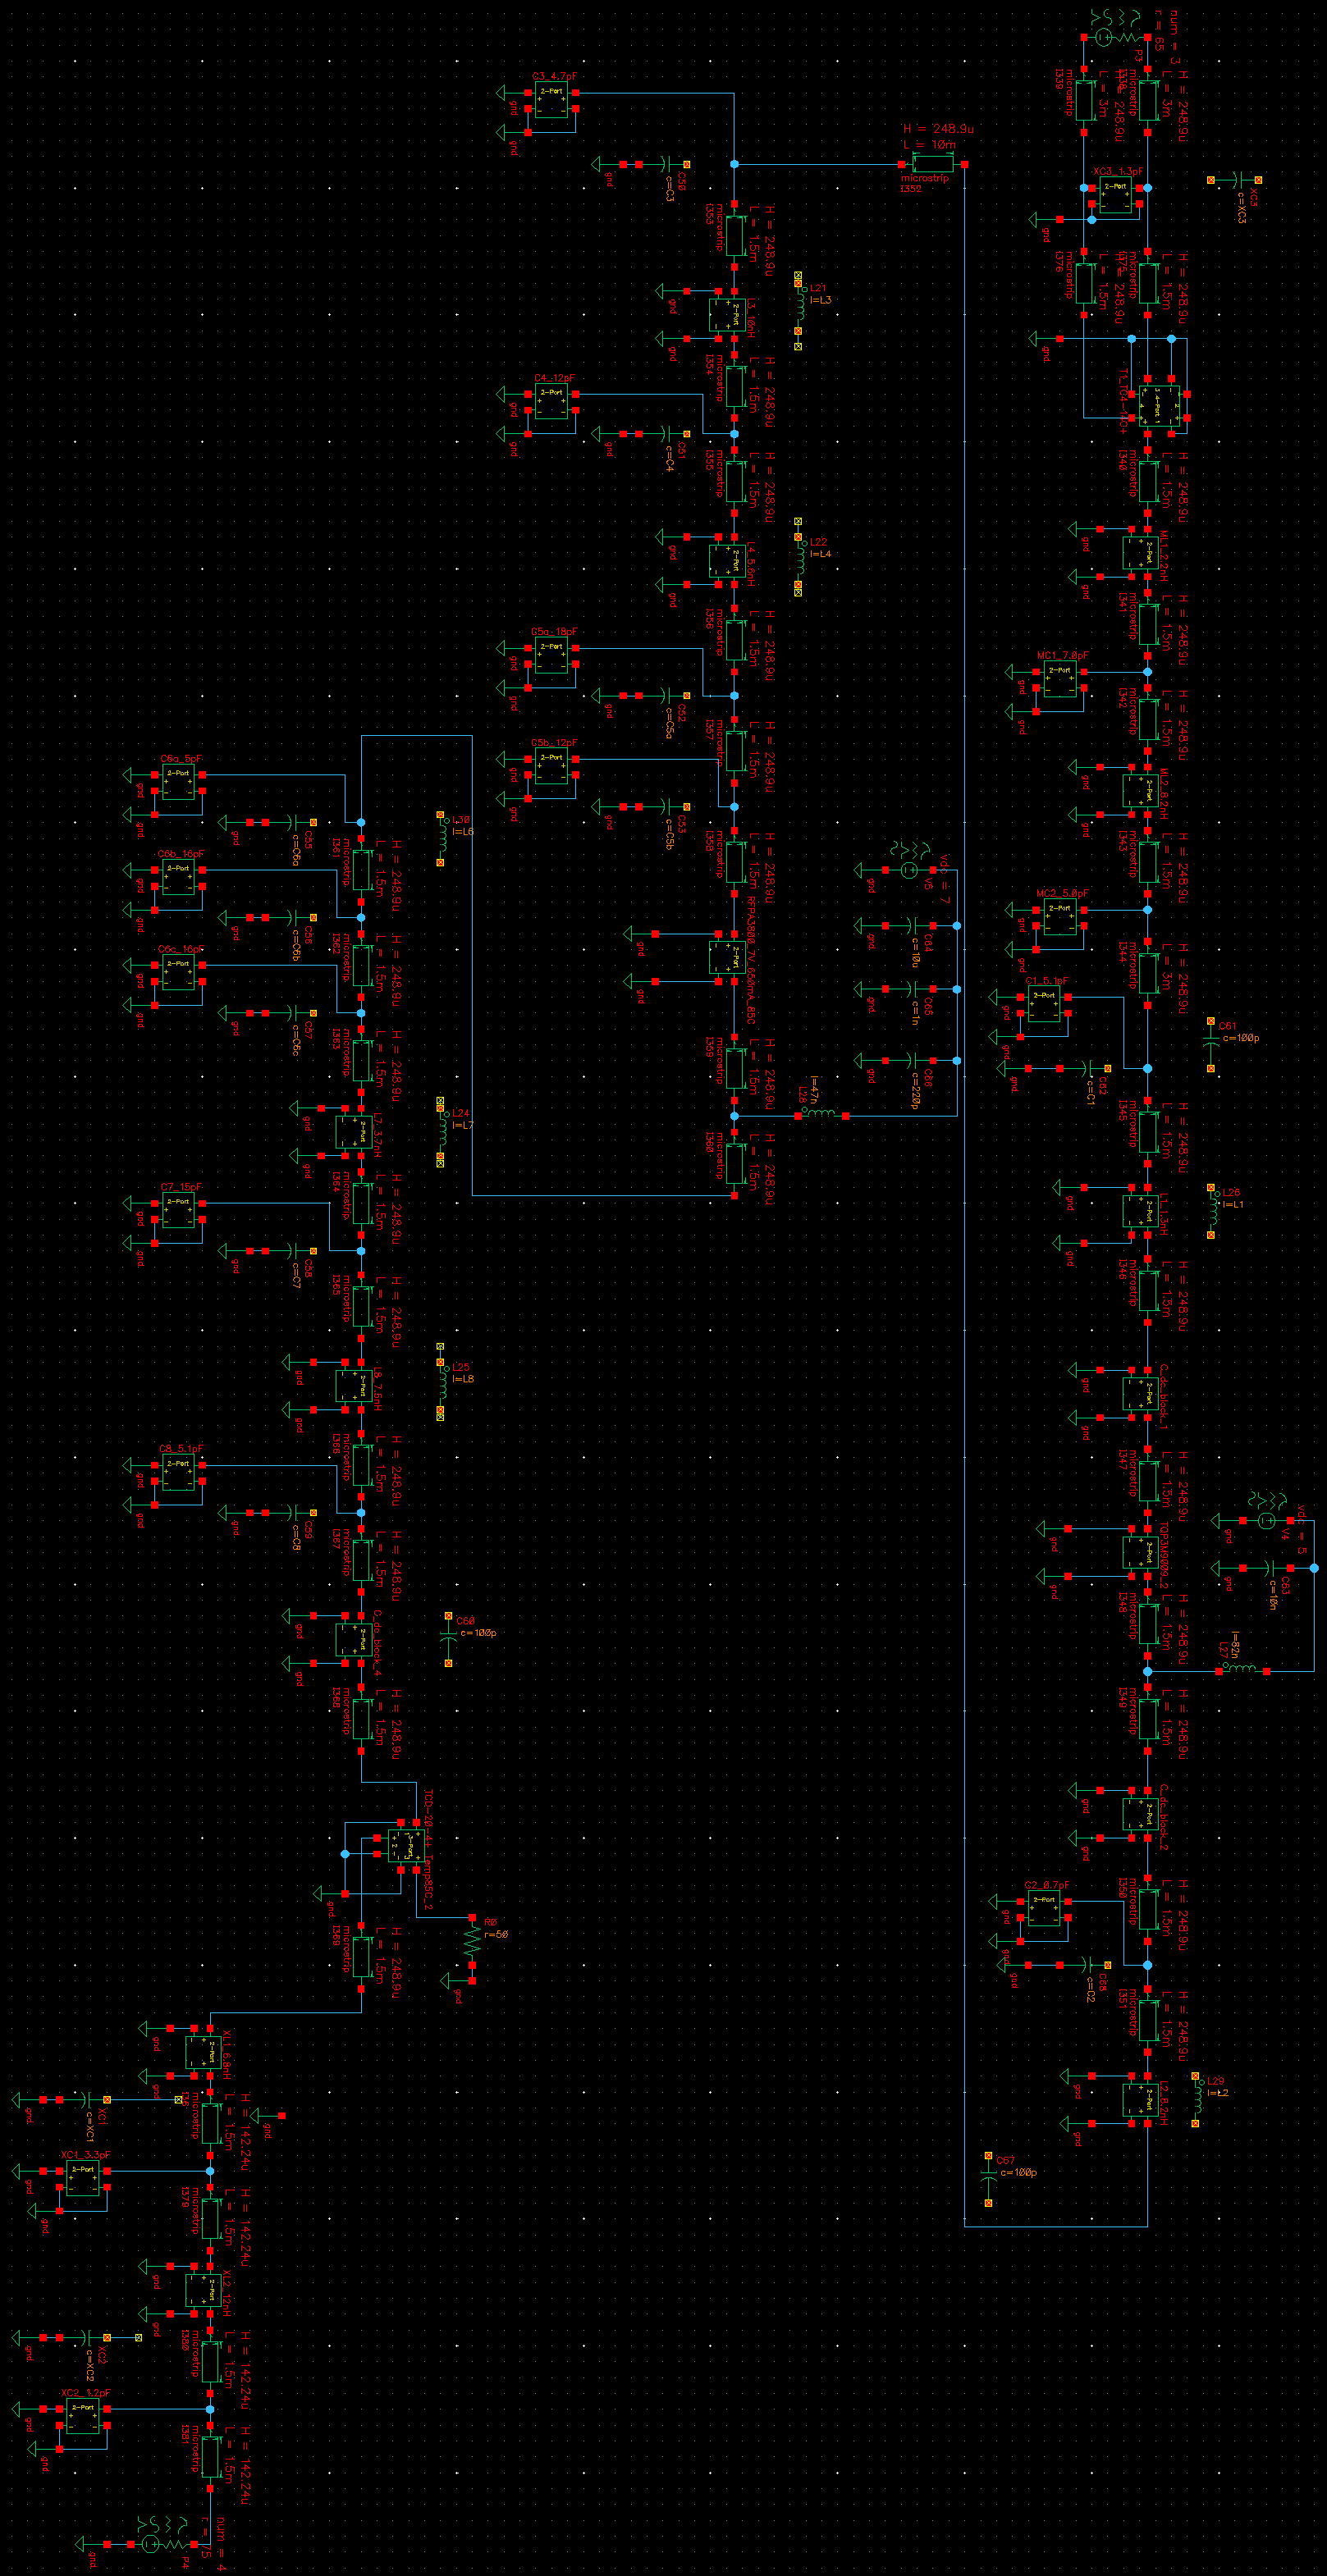
\includegraphics[width=0.75\linewidth]{figs/matching/spectre_uhf_tx_complete_chain}   
    \caption{Simulation model of full UHF transmit chain in Cadence Virtuoso SpectreRF.}
\label{fig_spectre_uhf_circuit}
\end{figure}
% PAGEBREAK  ^^^^^^^^^^^^^^

	The simulated results for the SpectreRF system in Figure~\ref{fig_spectre_uhf_circuit} are shown in Figure~\ref{fig_spectre_uhf_results}.
	Here, we present two results: 1) the gain performance of the system where each lumped element is replaced with an ideal capacitor or inductor while all other active components, switches, and traces are modeled by their empirical representations with parasitics (red); and 2) the gain performance when each ideal component has been replaced with an empirical S-parameter model and hand-tuned individually to bring performance as close to the ideal as possible (green).
	
	The hand-tuning procedure is inherently greedy but produces satisfactory results: 
	\begin{itemize}
		\item \textbf{Step 1}: select an arbitrary ideal component, replace the ideal component with its S-parameter small-signal model;
		\item \textbf{Step 2}: replace this component with the small-signal model for a component with a smaller or larger common value (\emph{e.g.} a 9~pF capacitor would be compared with a 10~pF and 8~pF component in this step);
		\item \textbf{Step 3}: select the component with system frequency response that is most like the ideal system frequency response, set this component selection;
		\item \textbf{Step 4}: repeat from Step 2 until no improvement in the system frequency response is gained;
		\item \textbf{Step 5}: repeat from Step 1 until all ideal components have been replaced with small-signal models.
	\end{itemize}
	
	Since there are generally fewer inductor step sizes in commonly-available \ac{SMT} components than capacitor step sizes, we perform the greedy tuning algorithm first on all of the inductors in a model and \emph{then} on the capacitors.
	
	We can see that the final circuit frequency response in Figure~\ref{fig_spectre_uhf_results} has good, flat performance with only 4~dB ripple from 470 - 750~MHz, and that the modeled gain diverges by 2-3~dB from ideal modeled performance primarily at the high frequencies above 550~MHz.
	The overall system gain in the SpectreRF simulation in Figure~\ref{fig_spectre_uhf_results} is smaller than that predicted by XSPICE in Figure~\ref{fig_spice_results}, but it also considers losses from component parasitic resistances, switch and filter insertion loss, and microstrip losses and is closer to that of the physical circuit realization.
	
%##################################################
\subsubsection{Evaluation of Broadband Matching Networks with Parasitics}
\label{sec_wurc_parasitic_eval}
	
	Finally, having considered all physical impairments in our simulation model and after hand-tuning the simulated design, we realized this new circuit design in the first \ac{WURC} prototype shown in Figure~\ref{fig_wurc_versions} as the green PCB.
	Additional simple resistive impedance matches were made from the source LMS6002D 65~$\Omega$ differential to the system 50~$\Omega$ single-ended and from the system 50~$\Omega$ to the 75~$\Omega$ output antenna ports, but these were not difficult and the process is omitted here.

% SpectreRF simulation results
\begin{figure}[ht]
\centering
  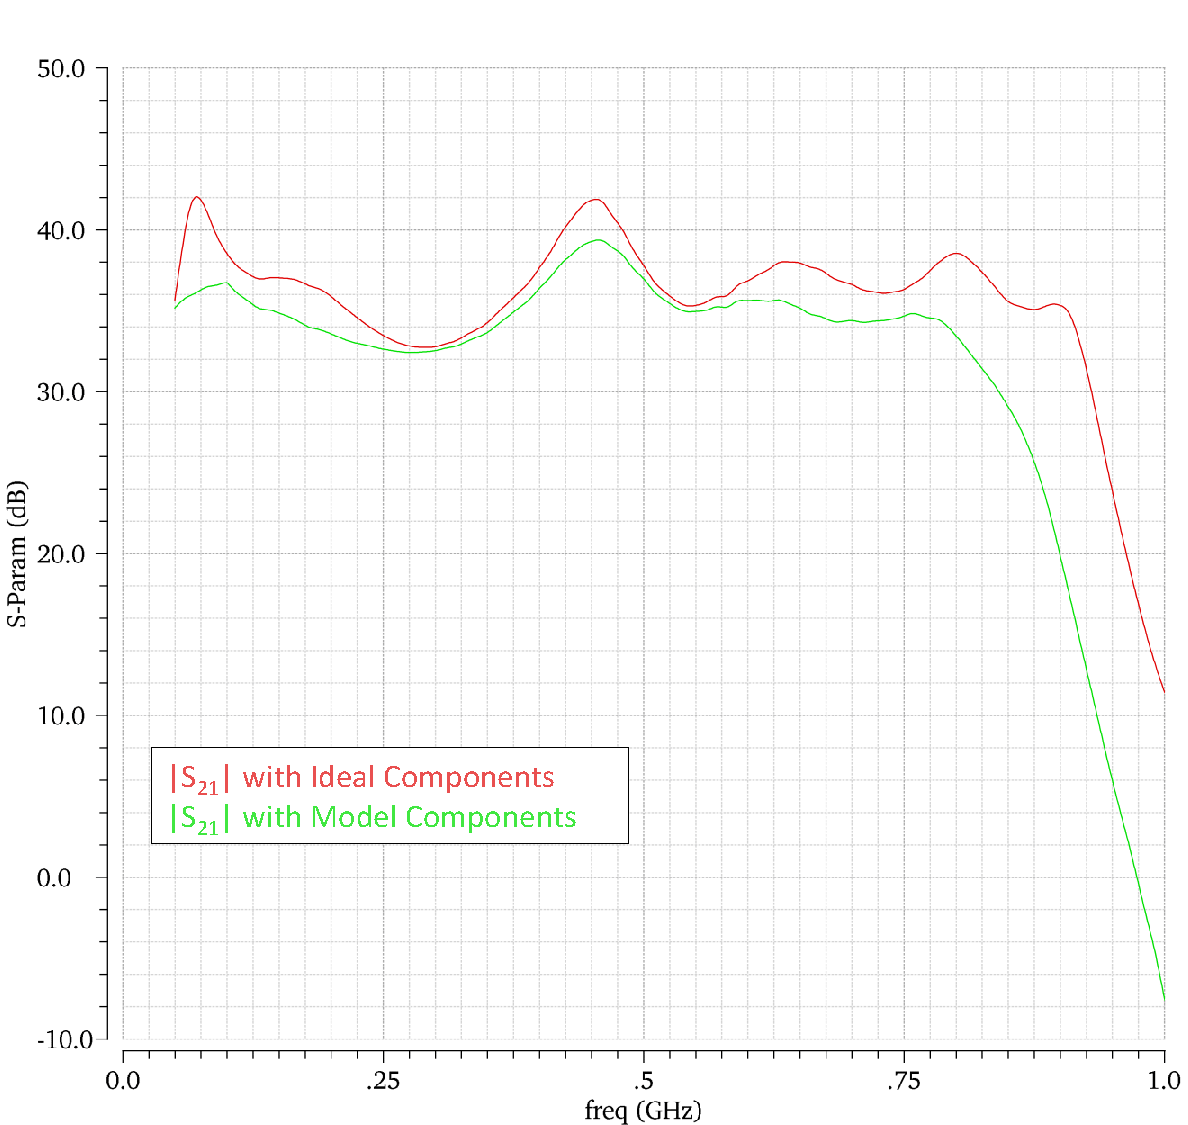
\includegraphics[width=0.7\linewidth]{figs/matching/spectre_simulation_results}   
    \caption{Simulated gain for the SpectreRF system in Figure~\ref{fig_spectre_uhf_circuit}.}
\label{fig_spectre_uhf_results}
\end{figure}
	

	In order to validate the final implemented design and understand how manufacturing process variation might effect the output frequency response of multiple RF chains in a \ac{MU-MIMO} system, we built a Python-based batch interface to the \ac{WURC}'s serial UART in order to sweep transmit frequencies while simultaneously controlling a bench-top vector signal analyzer to measure the output power \cite{guerra2012wurc_cal}.
	We implemented a digital frequency synthesizer within the digital baseband reference design for \ac{WURC} in order to generate a constant-power \ac{CW} complex sinusoid for ease of measurement.

% Output WURC power across multiple boards
\begin{figure}[ht!]
\centering
  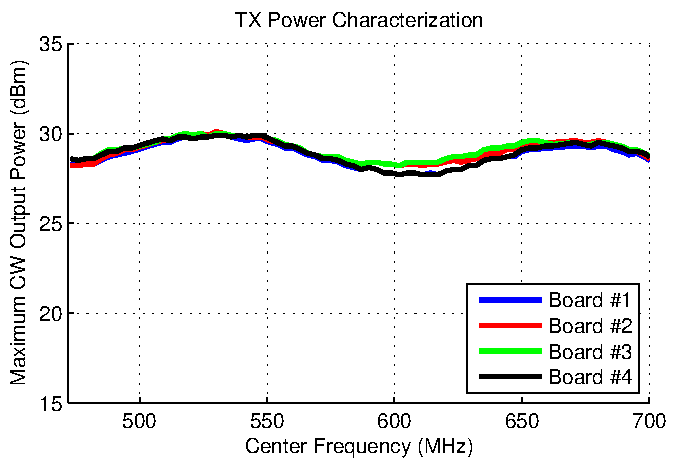
\includegraphics[width=0.8\linewidth]{figs/wurc/wurc_tx_power_plot}
    \caption{Maximum linear \ac{CW} output power as a function of center frequency for multiple \ac{WURC} units.}
		\label{fig_wurc_linear_power}
\end{figure}

	The process variation plot in Figure~\ref{fig_wurc_linear_power} was generated by increasing the output transmit gain of each \ac{WURC} at each center frequency until its output power amplifier began to saturate (\emph{i.e.} the last tested value where a 1:1 input:output gain relationship still held).
This is the delivered output power of \ac{WURC} just before the 1~dB compression point of the RF chain.
Notably, the process variation across different boards is less than 1~dB, with passband ripple on the order of 2.5~dB.
This means that multiple RF chains will maintain similar output power across the entire UHF frequency range, vastly simplifying system planning and gain control processes.

\subsection{Conclusion and Discussion}

	While this is a lengthy discussion, we believe there is valuable insight in presenting the step-by-step design and optimization of the \ac{WURC} broadband power transfer network as this work took years to develop and refine through various steps of manufacture and has application beyond this single design.
	We have attempted to not only provide enough information to replicate these design steps, but also provide motivation as to why certain decisions were made.
	%In addition, the real-frequency design code is also available open-source with permission from Yarman \cite{a_github_repo}.

	The final implemented UHF-band analog RF chain for \ac{WURC} provides up to 30~dB of static transmit gain, and up to 61~dB of dynamic receive gain, which combined with its on-board static \ac{LNA} can provide up to 83~dB of receive gain for improved sensitivity, although noise figure considerations generally limit this application to 72~dBm of dynamic receive gain.

 While we present a direct comparison of different manufactured \ac{WURC} boards demonstrating their consistent performance in Figure~\ref{fig_wurc_linear_power}, today we have manufactured dozens of \ac{WURC} boards with consistent results and also hundreds of related radio modules that utilize this same broadband power transfer design techniques for a wide range of operational frequencies and components.
	
	In conclusion, we find that the original real frequency circuit synthesis technique doesn't capture physical implementation tradeoffs well and made several changes to the design technique in order to improve the chance for success of the physical circuit realization:

\begin{enumerate}
	\item Instead of cascading multiple amplifier blocks in a series of dependent optimizations as proposed by Yarman \cite{yarman1982simplified}, we instead match the input and output of each amplifier to 50~$\Omega$ as proposed in our Section~\ref{sec_srft_problem_statement} problem statement and cascade them into each other. This allows us to decouple the design and optimization of the broadband matching network for each component and avoid the need to accurately model the microstrip feeds between amplification stages so long as they are placed in a nominal 50~$\Omega$ system.
	
	\item We utilize a simulation environment that either explicitly models package, pad, and trace parasitics or utilized empirical S-parameter models for linear system analysis. These types of tools are able to model and highlight implementation issues that are not apparent from the ideal circuits synthesized by the real frequency technique. Specifically, we present an example using Cadence Virtuoso SpectreRF in this thesis and currently use Keysight Genesys for this purpose.
	
	\item Finally, we add an additional hand-optimization step that utilizes linear analysis tools like SpectreRF or Genesys to adjust real component values based on their packages and parasitic properties in order to tune the physical circuit so that it approaches the ideal synthesized behavior. Today this is done in a greedy method whereby each component is individually hand-optimized, however the roadmap for future work to automate this with a discrete non-linear optimization algorithm using a library of empirical parts data is clear.
\end{enumerate}
	%##############################################################
\section{Fast Automatic Gain Control for SDR Systems}
\label{wurc_agc}

In radio communications, receivers must tolerate a wide range of input power levels in order to accommodate both near and distant transmitters; this effect is aggravated in large-scale UHF systems.
For example, the free-space path loss for a 400~MHz system operating over 10~km is $(\frac{4\pi d}{\lambda})^{2} = 104.5$~dB. This can present serious problems to the \ac{ADC} subsystem of a software-defined radio receiver if it must be capable of decoding signals from both nearby transmitters and those at a distance.

Intuitively, imagine a noisy room where one guest is yelling through a megaphone into your ear while another is whispering quietly in a corner; it would be difficult to understand what they were saying in either case.

Technically, the cause of distortion in a strong signal comes from the inability of an \ac{ADC} to distinguish between input voltage levels above and below its maximum and minimum codeword values.
This results in a phenomenon called \textit{clipping} where the analog signal is limited in its digital representation to the upper and lower bounds of the \ac{ADC} codeword, thus destroying information in the signal.
When the \ac{ADC} encounters this condition, we call it \textit{saturated}.

For a weak signal, distortion is generated when variation in the input signal is smaller than the minimum resolution of the \ac{ADC} or it becomes indistinguishable from systemic noise in the receiver.
Under these conditions, we say the signal is below the resolution of the \ac{ADC} or \textit{under-resolved}.

In addition, the amount of \ac{ADC} quantization error is proportional to the relative size of the quantization steps and the power of the signal of interest \cite{middleton2007agc}.
Thus, there is incentive to ensure that the power of the input signal is as large as possible without saturating the \ac{ADC}.

\ac{AGC} systems attempt to estimate the power input to a radio receiver and adjust the analog gains of that receiver in order to ensure that the \ac{ADC} input signal power falls within an optimal window and is not saturated while ensuring sufficient resolution available for the signal of interest.

\begin{figure}[t] % Idealized AGC block diagram
\centering
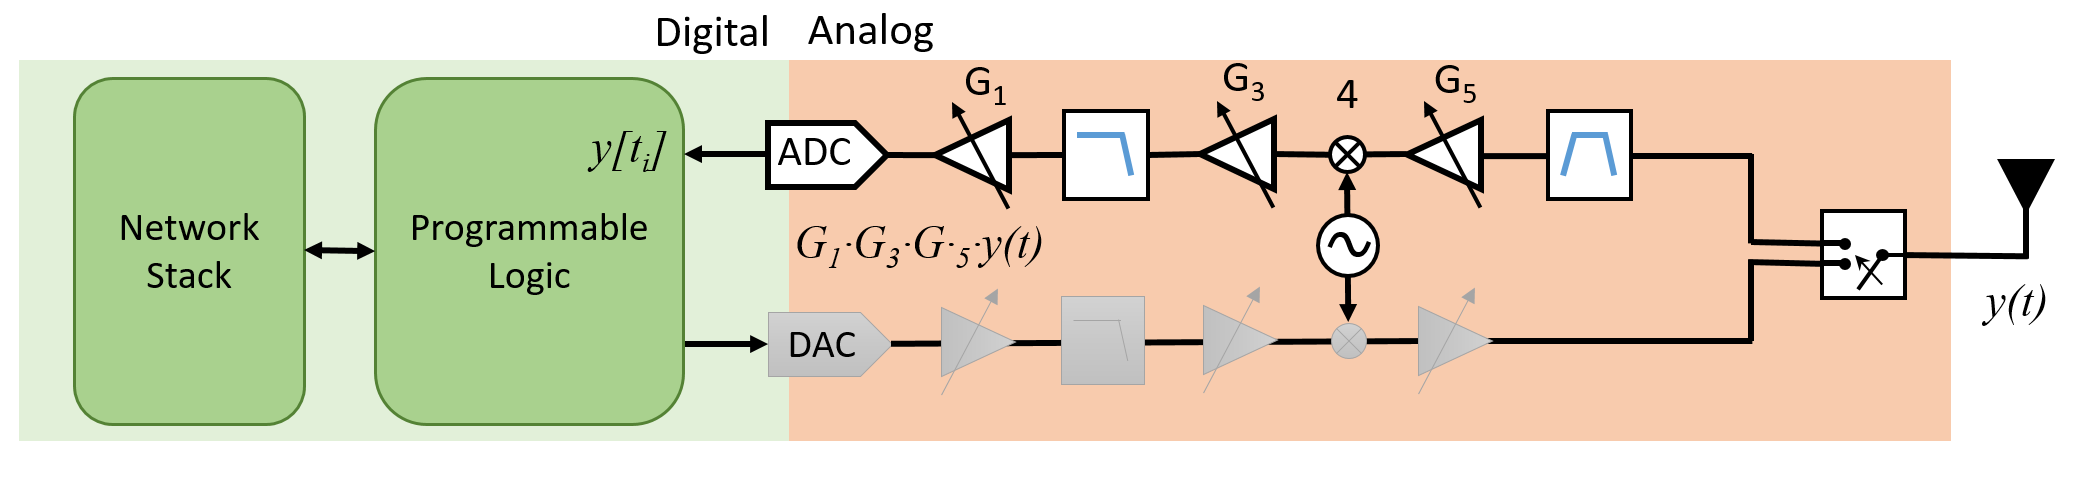
\includegraphics[width=1\linewidth]{./figs/agc/agc_rx_diagram}
\caption{Block diagram of the software-defined radio receive chain.}
\label{fig_sdr_ideal_rx}
\end{figure}

Figure~\ref{fig_sdr_ideal_rx} shows our block diagram of a generic software-defined radio system's receive chain with three programmable gain blocks: pre-mixer $G_5$, post-mixer $G_3$, and post-filtering $G_1$ that together control the input gain to the \ac{ADC}.
Under ideal conditions, when the input signal $y(t)$  is perfectly band-limited and all components are linear, the signal present at the \ac{ADC} input, $G_1\cdot G_3\cdot G_5\cdot y(t)$, will be converted to a digitally sampled signal, $y[t_i]$, that contains the full information present in the input signal $y(t)$.

In this section, we present the design, hardware implementation, and over-the-air validation of a new \emph{analog} \ac{AGC} subsystem designed for the \ac{WURC}.
This \ac{AGC} subsystem is novel in that it does not require the assistance of an external analog power estimation block and can therefore be implemented on any \ac{SDR}, yet it can still converge rapidly within the strict time constraints of common random-access communications standards such as IEEE 802.11 \cite{std11_2012}.
This differs from \ac{AGC} systems implemented on other \ac{SDR} platforms such as WARP \cite{middleton2007agc, warp} or SORA \cite{sora} that respectively utilize other analog circuitry or have a slow update loop limited by software processing times.

This novel architecture enables the implementation of critical \ac{AGC} functionality in systems that may be limited in analog hardware yet have sufficient real-time digital resources to implement our solution.

%#######################################
\subsection{AGC Design Specification}

The design goal of our \ac{AGC} system is to adjust the receive gains in our system such that any incoming packet with \ac{RMS} power between $[-103.6, -15.1]$~dBm at the input antenna port will have \ac{RMS} power between $[-42.6, -15.1]$~dBm when it reaches the \ac{ADC} as shown in Figure~\ref{fig_sdr_ideal_rx}.
Convergence to stable recieve gain values should be complete within $5.6~\mu s$ after reception of a inbound data packet.
We consider this ``fast'' \ac{AGC} since the gain is being dynamically adjusted on a symbol-level timescale ($\mu s$) rather than a packet timescale ($ms$).
In fact, we will see how many architectural decisions are guided by this relatively short timeframe.

These particular values are selected based on the parameters of the \ac{WURC} transceiver hardware \cite{lime2012lms6002d} and the expected characteristics of our signal waveform \cite{perahia2013next}; however the following design procedure can generally be applied to any \ac{SDR} system.

%=========================
\subsubsection{ADC Dynamic Range}
\label{sec_adc_dyn_range}

\begin{figure}[h] % AGC Design Diagram
\centering
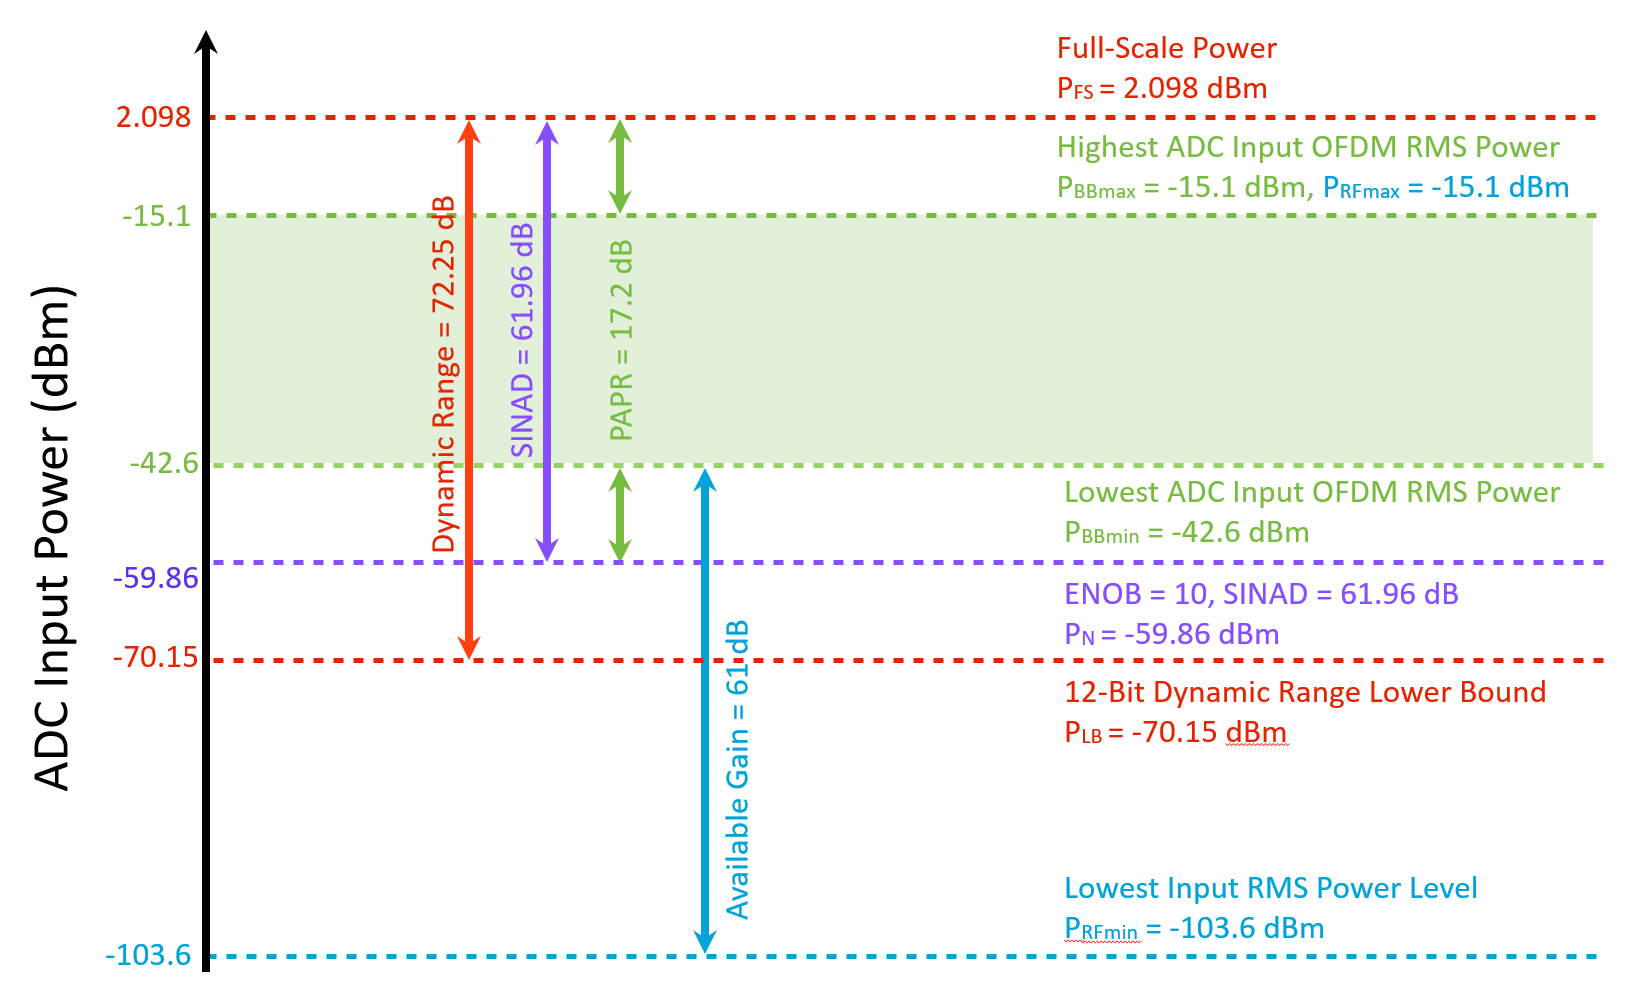
\includegraphics[width=1\linewidth]{./figs/agc/agc_dynamic_range}
\caption{Illustration of AGC resolution, system available gain, and signal dynamic range for the LMS6002D \cite{lime2012lms6002d}.}
\label{fig_agc_dynamic_range}
\end{figure}

\ac{ADC} components are characterized by their \ac{ENOB}, or the number of bits available for the digitization of signals after accounting for the systemic noise generated by the \ac{ADC} circuitry, and their \ac{FSR}, or the minimum and maximum voltage values that can be encoded by the \ac{ADC}.
These two values provide the lower and upper bounds, respectively, of the \ac{ADC} power resolution \cite{adi2008sinad}.
Since the voltage of an \ac{ADC} is measured across a static resistive load, voltage level bounds translate directly into power level bounds.

Formally, \ac{FSR} is defined as:
\begin{equation} \label{eq_fsp}
\text{FSR} := P_{FS} = \frac{V_{MAX}^2}{R_{ADC}} = \frac{(1.8)^2~\text{V}^2}{2000~\Omega} = 2.095~\text{dBm},
\end{equation}
where $V_{MAX}$ is the voltage of the maximum ADC codeword and $R_{ADC}$ is the value of the ADC load resistor in Ohms \cite{lime2012lms6002d}.

\ac{SINAD} is defined as the ratio of the desired signal to noise and distortion from all sources excluding the power of the DC spectral component \cite{adi2008sinad}.
As an empirically determined specification, it captures the practical dynamic range of an ADC by incorporating ADC non-linearities and distortions and indicating the level at which a desired signal would become indistinguishable from interfering signals.
When the input signal is a full-scale sinusoid, it is related to the \ac{ENOB} according to the following relationship that follows from the definition of an ideal ADC \cite{rohde2011enob}:

\begin{equation} \label{eq_enob}
\text{SINAD} := \text{ENOB} \cdot 6.02 - 1.76~\text{dB}.
\end{equation}

The \ac{SINAD} is plotted in Figure~\ref{fig_agc_dynamic_range}, where it defines the operational range of the \ac{ADC}.

%===========================
\subsubsection{Peak-to-Average Power Ratio}
\label{sec_agc_papr}

The 802.11ac and 802.11af standards define a high throughput mode that utilizes \ac{OFDM} waveforms for physical-layer communication \cite{perahia2013next, flores2013ieee80211af}.
Due to the statistically independent nature of the symbols transmitted on each subcarrier, the overall time-domain signal of a wideband \ac{OFDM} waveform with many subcarriers may be modeled as a zero-mean random Gaussian process \cite{proakis1995digital}.
Modeled thus, the ratio of the highest power time-domain sample to the mean time-domain sample grows with the variance of the aggregate Gaussian process, or grows with $\sqrt{K}$, where $K$ is the number of subcarriers.

When a signal is represented as a series of time-domain complex values, $s[t_i]\in \mathbb{C}$, indexed by time $t_i$, we can define the \ac{PAPR} \cite{bauml1996reducing}: 
\begin{equation}
\text{PAPR} := 10 \cdot\log_{10}(\frac{\max_{i}(|s[t_i]|^2)}{\mathbb{E}\{|s[t_i]|^2\}}).
\end{equation}

For 802.11af, a 20~MHz VHT frame contains 52 subcarriers, resulting in a worst-case \ac{PAPR} of approximately 17.2~dB.
In order to guarantee that reception of this signal can take place without clipping at the ADC, the input power at the ADC should be less than 17.2~dB below the ADC's \ac{FSR}.
Similarly, in order to guarantee that time-domain samples are not under-resolved, the input power to the ADC should be more than 17.2~dB above the ADC's effective noise floor (FSR - SINAD).
These two additional \ac{PAPR} margins (green) are illustrated in Figure~\ref{fig_agc_dynamic_range} to yield the target operational range of the ADC (shaded green region).

Other literature has focused on how the \ac{PAPR} of signals may be reduced with digital pre-processing steps \cite{bauml1996reducing}, however we assume these techniques will not be applied to the standard 802.11af waveform.
If \ac{PAPR} mitigation techniques, also know as \emph{crest-factor reduction}, are utilized, this will simply decrease the required \ac{PAPR} margin in our design accordingly.


%===========================
\subsubsection{AGC Timing Constraints}
\label{sec_agc_timing}

	A necessary condition for generic fast analog gain control to be feasible is that the digital logic must be able to react to and effect changes in the analog gain blocks within the deadline allowed for \ac{AGC} operations.
	This becomes particularly important in random-access systems like 802.11 since the receiver generally doesn't have information about the transmitter until after its signal is already being processed and therefore must rapidly adapt reception parameters in order to detect and decode the received packet accurately.

	Perhaps the most challenging requirement of the \ac{WURC} AGC system design is that of meeting the strict 802.11af/ac frame timing.
	In this section, we analyze the timing constraints of our particular \ac{SDR} system and what this means for other system implementations of our fast \ac{AGC} system.

\textbf{Frame Preamble Timing.} The \ac{PLCP} component of the 802.11 standard defines a common preamble for packet transmissions that enables receiving devices to synchronize to the transmitted waveform \cite{perahia2013next, 80211ac} and simplifies interaction with higher layer of the network stack.
	Displayed logically in Figure~\ref{fig_agc_80211_plcp}, the \ac{PLCP} consists of two training fields of $8~\mu s$ for receiver synchronization and a \emph{SIGNAL} field of $4~\mu s$ containing rate and data length information for the rest of the packet or \ac{PPDU}.

\begin{figure}[h] % Idealized AGC block diagram
\centering
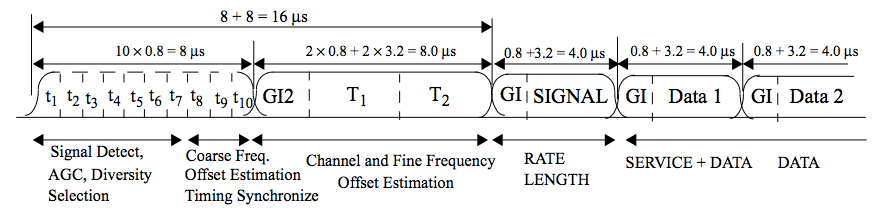
\includegraphics[width=1\linewidth]{./figs/agc/agc_80211_plcp_format}
\caption{IEEE 802.11-2012, \S18.3.3 \ac{PLCP} preamble format and timing \cite{std11_2012}}
\label{fig_agc_80211_plcp}
\end{figure}


	While precise receiver operation is not specified in the 802.11 standard, generally the first 7 sub-fields of the short training field, L-STF, are reserved for packet detection, gain control, and antenna diversity selection.
	The fields are labeled $t_1$ through $t_7$ in Figure~\ref{fig_agc_80211_plcp}.
	The remaining 3 fields of the L-STF and the long training fields, L-LTF, are reserved for timing recovery, channel estimation, and transmitter frequency offset calculation \cite{perahia2013next}.

	In this particular \ac{SDR} realization, that means that incoming packets must be detected and gains must be dynamically set within $5.6~\mu s$ in order to meet the timing constraints given in the 802.11 standard.
	For 40~MHz \ac{ADC} sampling rates, that's less than 224 samples since the \ac{AGC} system must perform signal processing; at 20~MHz sampling rate, the system must react with less than 112 samples of data.

\textbf{Serial Interface Timing.} The LMS6002D transceiver containing the receive variable-gain amplifiers is controlled by a \ac{SPI} controller accessing an 8-bit command register space \cite{lime2012lms6002d}.
	Each write command consists of an 8-bit instruction concatenated with an 8-bit data payload.
At a maximum interface speed of 50~MHz, it takes $0.32~\mu s$ to complete each \ac{SPI} transaction.
	Gain settings for the LMS6002D transceiver require \ac{SPI} transactions to three separate registers; however, we observe that one register controls the first-stage \ac{LNA}, which should always be left active for noise performance and should therefore not be adjusted by the \ac{AGC} system.
	Since it take approximately 100~$ns$ for the receive gain stages to settle once programmed, we can expect at least 0.74~$\mu s$ of delay for each change in receive gain to be implemented, or around 14\% of the total timing budget allowed.

	In general, our design for an analog \ac{AGC} system must be able to set receive gains several times within the time budget allocated since it can not rely on saturated digital observations to estimate the input power to the \ac{ADC}.
	Other commercial \ac{SDR} platforms (\emph{e.g.} based on AD9363, ADRV9009, or LMS7002M transceivers \cite{adi2016ad9363, adi2018adrv9009, lime2018lms7002M}) operate on similar timescales with respect to digital control interfaces, making our design feasible across a wide range of SDR platforms.


%##############################################################
\subsection{Alternative AGC Architectures}
\label{sec_agc_related}

In this section, we present a detailed comparison of our approach with alternative \ac{AGC} systems used in other commercial \ac{SDR} systems.

\subsubsection{Digital Gain Control}
\label{sec_agc_dig_alt}

\begin{figure}[h] % AGC Design Diagram
\centering
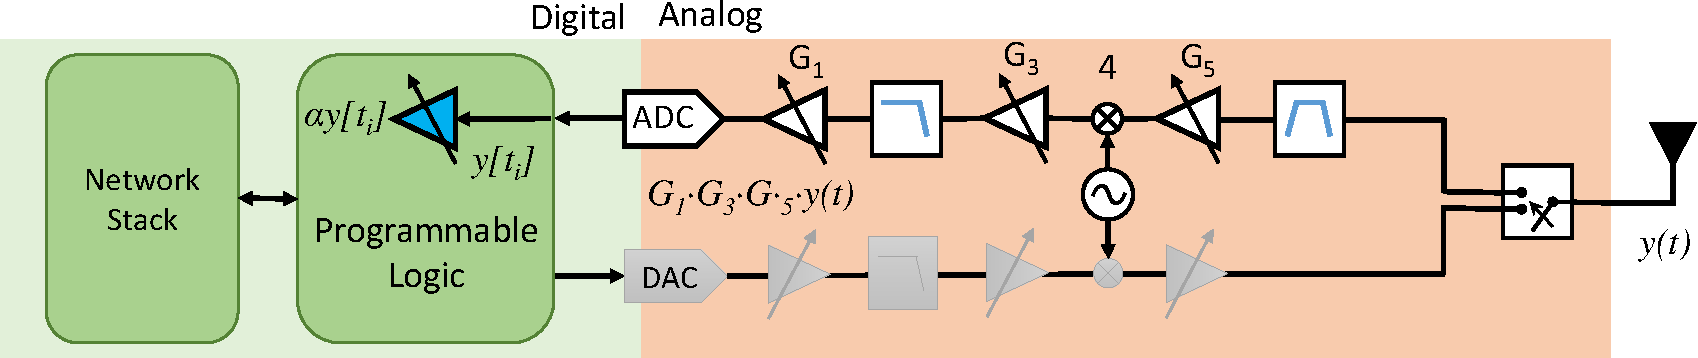
\includegraphics[width=0.9\linewidth]{./figs/agc/agc_digital_diagrams}
\caption{Diagram of digital gain control circuitry (blue).}
\label{fig_dig_agc_diagram}
\end{figure}

	When \ac{DSP} processing blocks are designed with fixed point precision, it is sometimes critical to ensure that the input \emph{digital} signals do not exceed certain minimum or magnitude bounds in order to avoid numerical precision errors or overflow.
	For that reason, \emph{digital} automatic gain control is often implemented in radio systems in order to ensure the integrity of downstream fixed precision processing blocks \cite{lee2006agc}.
	In Figure~\ref{fig_dig_agc_diagram}, we show that these subsystems are generally implemented in the programmable logic of the \ac{SDR} with a digital gain block, providing a scalar gain of $\alpha$ multiplied with the digital IQ sample stream before being further processed. 
	
	However, once the baseband analog signal has been sampled at the \ac{ADC}, any chance to avoid under-resolved or clipped analog signals is lost, thus its utility is somewhat limited.
	Therefore, our approach of using digital feedback to control analog gain rather than digital gain can be used to meet both the requirement of reliable signal magnitude for fixed-precision \ac{DSP} blocks as well as analog signal power within the operational range of the \ac{ADC}.


\subsubsection{Analog Input Power Estimation}
\label{sec_agc_analog_alt}

\begin{figure}[h] % AGC Design Diagram
\centering
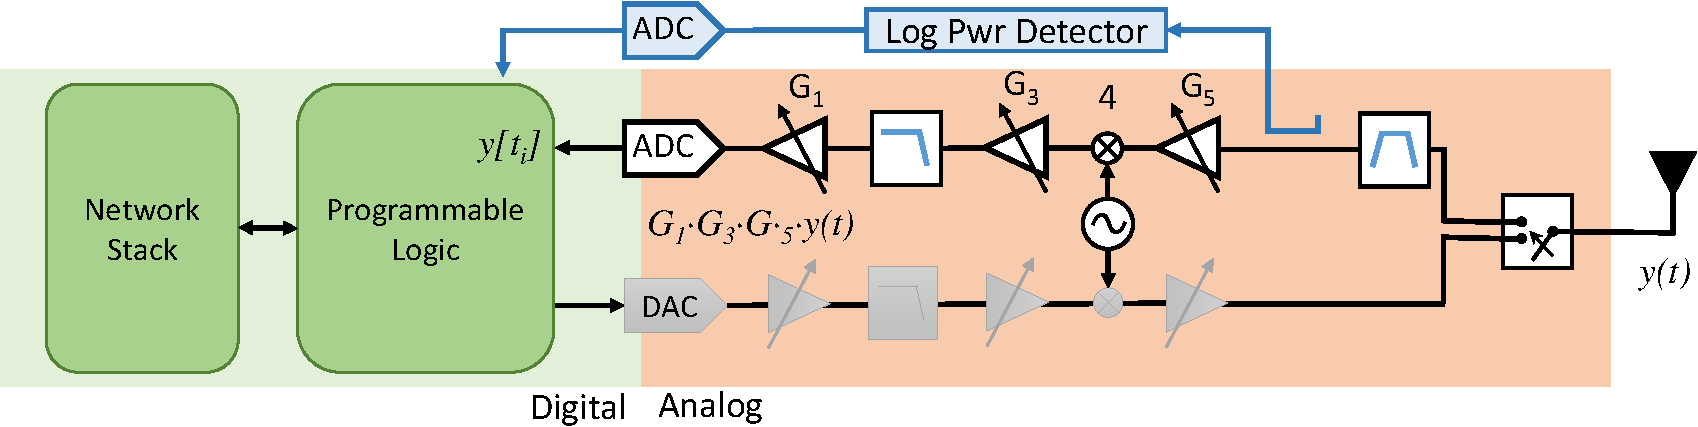
\includegraphics[width=0.9\linewidth]{./figs/agc/agc_diagrams_analog}
\caption{Diagram of analog power detection circuitry (blue).}
\label{fig_pwr_detection_diagram}
\end{figure}

	The most commonly used alternative architecture for analog gain control for \acp{SDR} is to directly estimate the input power to the \ac{SDR} at the input antenna port using a power coupler,\footnote{Alternatively, this estimation can take place at any point along the receive chain, provided gains between the measurement point and the input to the \ac{ADC} are known.} log power detection circuitry, and an auxiliary \ac{ADC} to convert the sensed analog power to a digital representation Figure~\ref{fig_pwr_detection_diagram} (blue).

	When designing \ac{WURC}, we first implemented analog power detection in our first development PCB prototype.
In Figure~\ref{fig_pwr_detection_proto}, we show a prototype analog gain control circuit utilizing a Maxim MAX2015 log-power detector and the built-in \ac{ADC} within the Stellaris microcontroller (bottom right PCB).
This same architecture was used to develop the Lime Microsystems LMS6002D control library \cite{guerra2013lms6002d}.

\begin{figure}[ht] % AGC Design Diagram
\centering
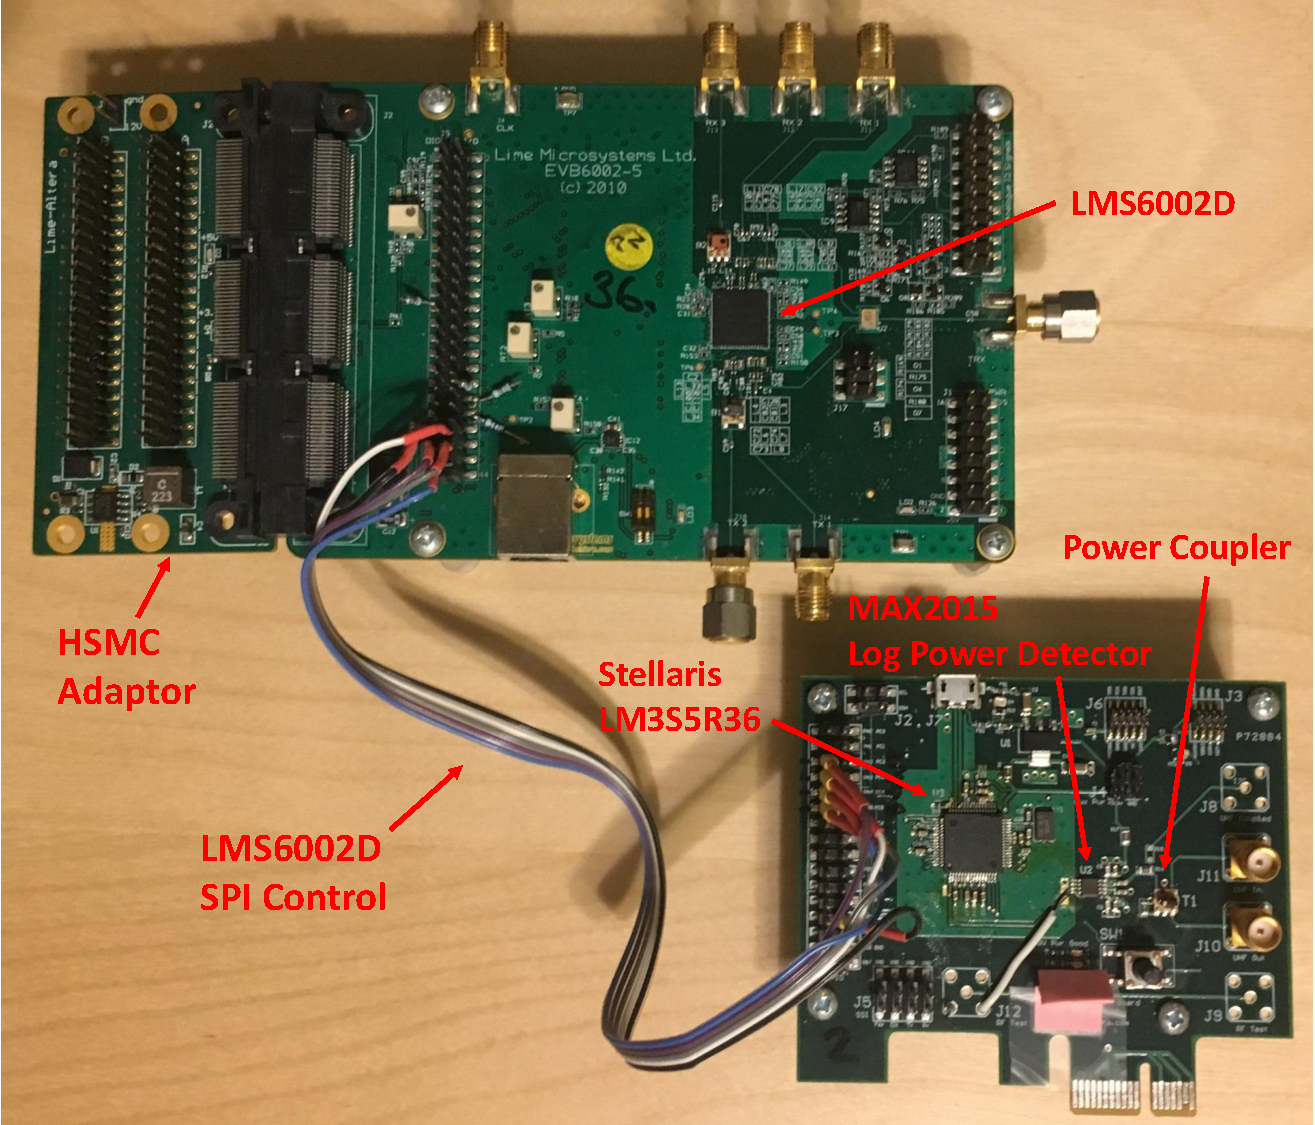
\includegraphics[width=0.9\linewidth]{./figs/agc/agc_dev_board}
\caption{Prototype analog log-power detector and LMS6002M development PCB.}
\label{fig_pwr_detection_proto}
\end{figure}

Three challenges were encountered:
	First, the extra analog power estimation components require additional cost and impose constraints on circuit layout and signal integrity.
	Second, and more subtlety, the division of gain control logic between multiple components requires synchronization and overhead that begins to eat into the \ac{AGC} timing budget.
For example, in our implementation, the Stellaris LM3S5R36 required a significant delay to estimate input power, make receive gain and packet detection decisions, and issue gain setting commands to the LMS6002D transceiver.
	Third, the MAX2015 has a dynamic detection range between -65 and +5~dBm, whereas we already expect to support packet reception well below -65~dBm.
	An additional RF amplifier could be provisioned to boost the detector input level or the RF coupler could be inserted somehow after various gain stages, however the former approach would add additional system cost and the latter was not possible with our highly-integrated LMS6002M transceiver IC.

	Instead, by eliminating analog power detection circuitry and integrating these functions within the digital \ac{SDR} logic in our proposed design, we reduced the overall cost and complexity of the radio design and provided tighter integration of \ac{DSP} logic and gain control functions to improve reaction speeds.
	
		The most recent generation of \ac{SDR} transceivers are starting to integrate this type of analog power estimation circuitry \cite{adi2018adrv9009}; however, our final design can be implemented in legacy \ac{SDR} devices that don't provision analog circuitry, increasing the number of systems that can benefit from our approach while providing equivalent performance.

%##############################################################
%\subsection{Fast Hybrid Packet Detection}
%\label{sec_pkt_detection}
%
%\rgnote{Packet detection across a wide range on input signal levels is difficult with any one detection technique; thus we design a hybrid detector that uses both energy detection and cyclostationary detection (autocorrelation) to quickly detect an incoming packet reliably and trigger AGC.}
	%
%\begin{figure}[h] % AGC Design Diagram
%\centering
%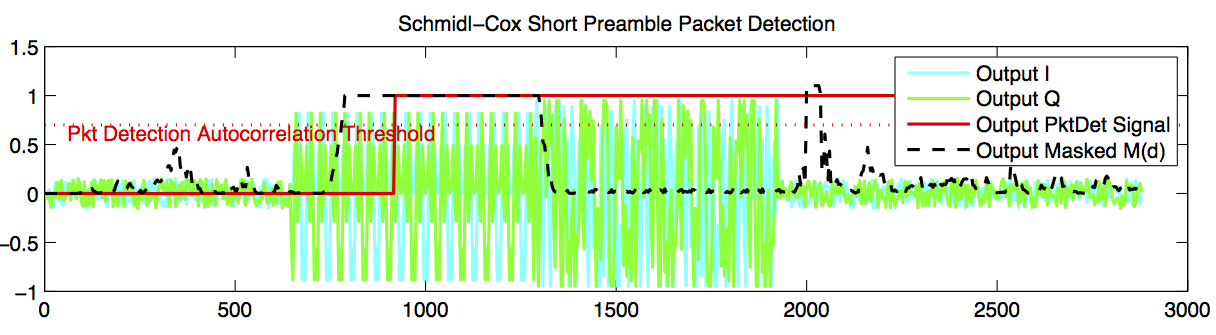
\includegraphics[width=1\linewidth]{./figs/agc/agc_schmidtl_cox_autocorrelation}
%\caption{Example of digital autocorrelation packet detection.}
%\label{fig:agc_autocorr}
%\end{figure}
%
%A key observation is that detecting a saturated  or strong input signal is more reliable and quicker than detecting an under-resolved or weak signal.

%##############################################################
\subsection{Hybrid Packet Detection}
\label{sec_pkt_detection}

	The challenge with implementing \ac{AGC} with only the input of the \ac{ADC} as a reference is that signals that fall outside of the ADC's dynamic range are unreliable.
	Taking the 802.11af standard as a reference, it may not only be difficult to detect the incoming packet when the digital samples are under-resolved or clipped, but any input power estimate will also be inaccurate since the digital samples are not capturing the full power of the incoming signal.

	Our solution is to approach this problem in steps: first, detect that a packet is being received; second, quickly detect and remove saturation with coarse gain steps; third, once saturation has been removed, fine-tune receive gains with a reliable estimate of the \ac{ADC} input power.

	The first step is addressed by utilizing the Schmidl-Cox digital packet and timing detection technique \cite{schmidl1997robust} for sensitivity in parallel with an energy detection block for quick packet detection.
	
\begin{figure}[ht] % Packet Detection Example
\centering
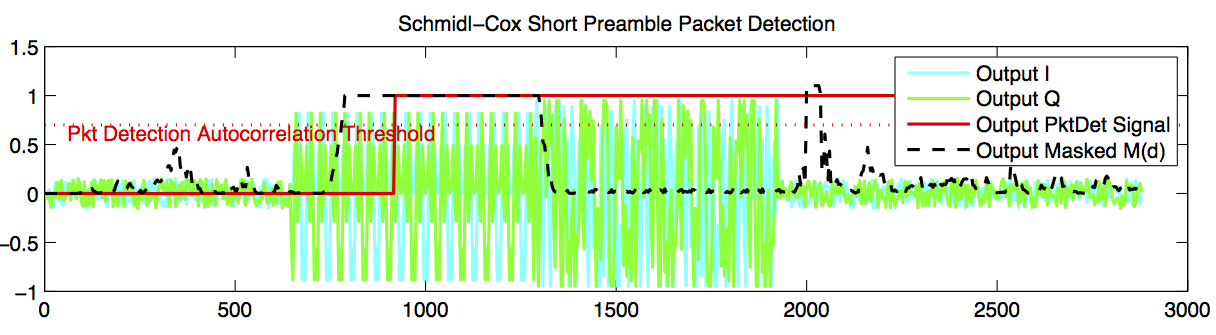
\includegraphics[width=1\linewidth]{./figs/agc/agc_schmidtl_cox_autocorrelation}
\caption{Example of digital autocorrelation packet detection.}
\label{fig_agc_autocorr}
\end{figure}
	
	The Schmidl-Cox detector works by auto-correlating the input signal and normalizing this result by the input power level in order to produce a large detection metric $M(d)$ when a repetitive signal with period equal to the 802.11 short timing sequence period is observed (0.8~$\mu$s, Figure~\ref{fig_agc_80211_plcp}).
	A simulation of digital packet detection using this method is shown in Figure~\ref{fig_agc_autocorr}, where the in-phase (I) and quadrature component (Q) are given in green and cyan, the auto-correlation metric value is shown in black, and the packet detection decision is shown in red (transition from $0 \rightarrow 1$).
	In order to reject false-positive packet detection, the Schmidl-Cox detector waits for the decision metric $M(d)$ to cross a threshold (red dotted line) for a specified period of time.
	
	Both the value of the threshold and the number of samples required to be above that threshold before deciding a packet is detect can be adjusted to tune the probability of a false-positive and missed-detection.
	We show the simulation in Figure~\ref{fig_agc_autocorr} at relatively low \ac{SNR} value in order to demonstrate that the Schmidl-Cox detector is relatively slow to produce a decision even under ideal conditions: by the time the packet detection signal is raised, over half of the 5.6~$\mu$s time budget for \ac{AGC} has been consumed.
	
	In contrast, a simple energy-based detection algorithm can react relatively quickly, during the first 0.8~$\mu$s, however it has fundamental detection limits for low-\ac{SNR} signals in the presence of noise \cite{shellhammer2006performance}.
	Our key observation is that energy detection works well and quickly for high-\ac{SNR} signals, which is when we will need additional time to remove potential \ac{ADC} saturation.
	In contrast, auto-correlation techniques perform well but respond slowly for low-\ac{SNR} signals, where we may expect little to no \ac{ADC} saturation.
	
	In our design, the packet detection is taken as the logical-OR of the detection output of both detectors, resulting in the best-case packet detection performance in both high-SNR and low-SNR regimes.
	The transceiver's idle receive state is initially set to maximum receive gain, ensuring that even weak packets will be detected reliably.

	%\rgnote{it really would be great to have a plot here showing detection probabilities or detection speeds for various detection methods... this could be actual hardware-in-the-loop or simulation, both are relatively easy.}

%##############################################################
\subsection{Coarse Gain Control for Saturation Removal}
\label{sec_coarse_gain}

	Once a packet is detected via energy or auto-correlation detection methods, we then wish to detect and remove \ac{ADC} saturation.
	Lee \emph{et. al.} \cite{lee2006agc} proposed a digital saturation detector aimed at adjusting the \emph{digital} gain level for fixed-precision digital logic in \ac{OFDM} transceivers.
	We utilize this same saturation detection logic in order to instead detect \emph{analog} \ac{ADC} saturation.
	Our implementation is presented in Figure~\ref{fig_agc_sat_block}, where the raw I and Q streams are independently observed for saturation conditions: crossing a magnitude threshold a specific number of times (3) within a window of 16 samples.
	If at any time more than 3 samples are observed above this conservative threshold, the input is declared ``saturated;'' however at least 16 consecutive samples must be observed after reset before the input can be declared ``not saturated.''

\begin{figure}[ht] % AGC Saturation Detection Block Diagram
\centering
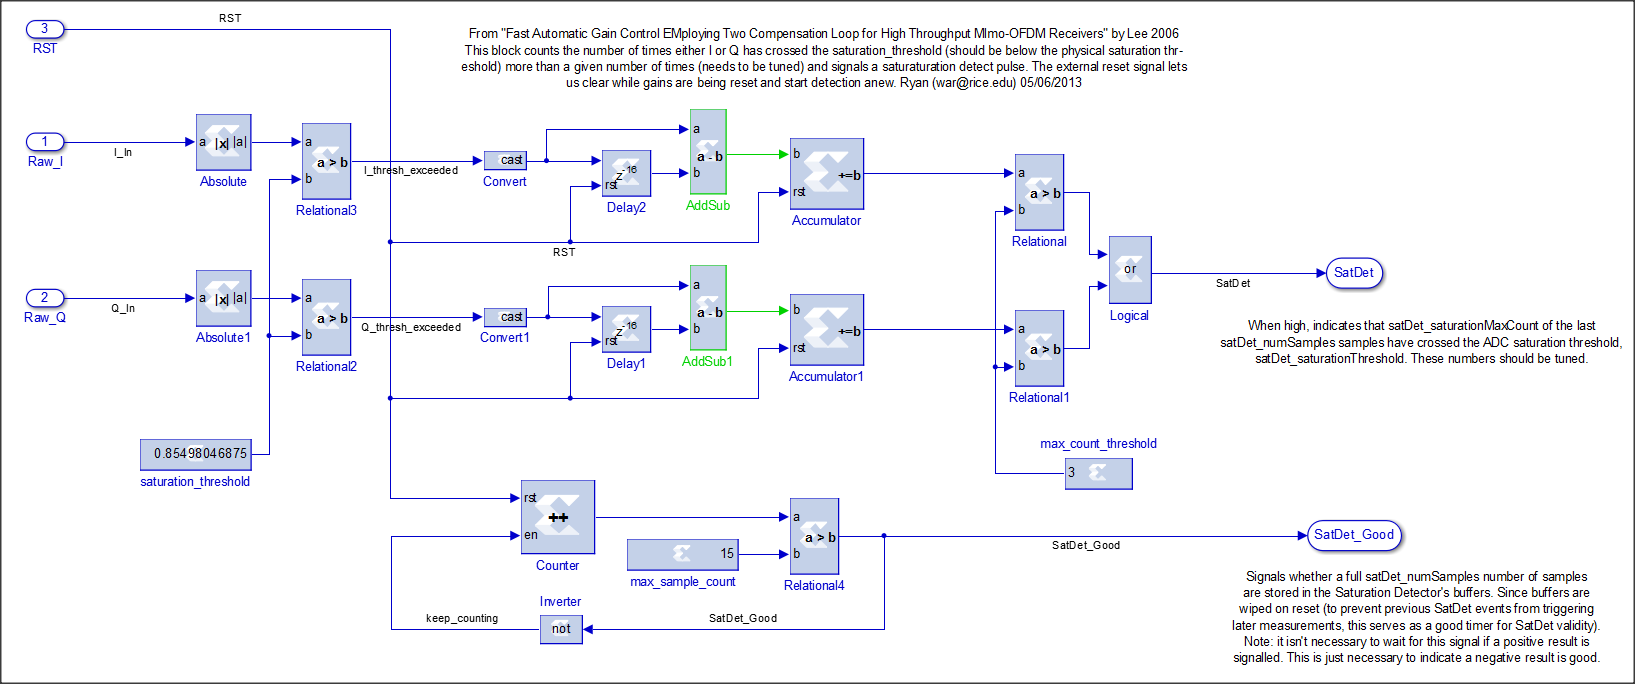
\includegraphics[width=1\linewidth]{./figs/agc/agc_saturation_block_implementation}
\caption{Digital logic block diagram implementation of ADC saturation detection.}
\label{fig_agc_sat_block}
\end{figure}

	Once saturation is detected, the analog receive gain is reduced in large steps to remove it.
	Since the ideal dynamic range of the \ac{ADC} is $[-15.1, -42.6]$ as per our calculations in Section~\ref{sec_adc_dyn_range}, we back off analog receive gains by 27~dB each time that saturation is detected on the \ac{ADC}.
	This results in decision regions as shown in Figure~\ref{fig_agc_coarse_gain}: if the input signal power falls within the green region from $[-103.6, -76.1 ]$ and the receive gain is set to 61~dB then we expect to detect no saturation and no coarse gain control cycles are required.
	Similarly, if the input signal power falls within the yellow region from $[-76.1, -49.1 ]$, then we expect saturation to be detected and one coarse gain fallback to 34~dB will be required, and so forth for the red region and purple region.
	
% AGC Coarse Gain Control Ranges
\begin{figure}[ht]
\centering
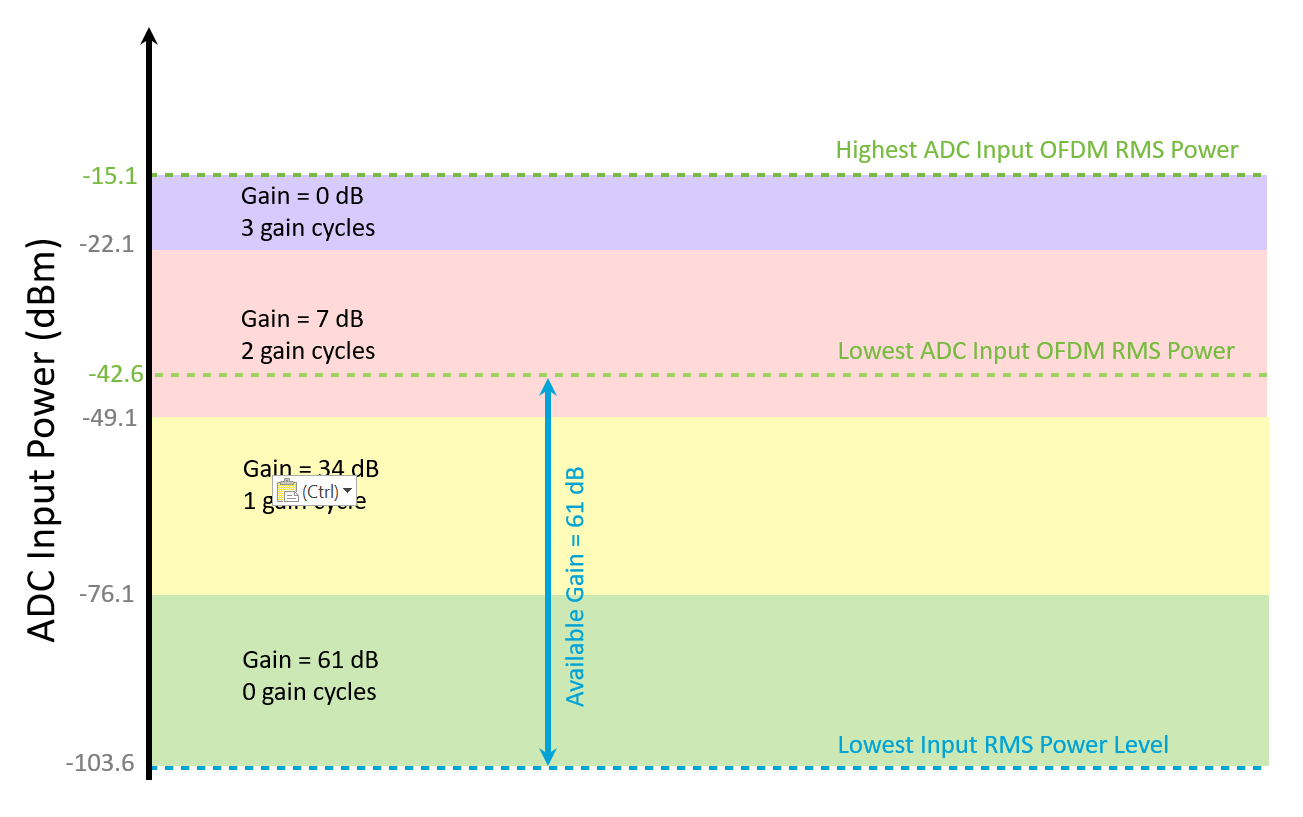
\includegraphics[width=1\linewidth]{./figs/agc/agc_control_ranges}
\caption{AGC input power regions for coarse gain control.}
\label{fig_agc_coarse_gain}
\end{figure}
	
	This entire sequence is governed by a digital Mealy state machine that is triggered upon a packet detection event.
	Implemented with lookup tables in \ac{FPGA} fabric, the AGC state machine flow diagram is given in Figure~\ref{fig_agc_state_machine}.
	Program execution begins once a packet is detected and a issues a trigger signal to bring the machine out of \emph{IDLE} state.
	The state machine then performs successive rounds of saturation detection and removal, entering the fine AGC state once saturation is removed.
	Once the fine gains have been set and a final power estimation round stores the settled input power level for higher layer control, the AGC state machine enters the \emph{IDLE} state, waiting for the next packet detection trigger.
	
	%====================== State Machine Diagram
%http://madebyevan.com/fsm/
\begin{figure}[p]
\begin{center}
\begin{tikzpicture}[scale=0.2]
\tikzstyle{every node}+=[inner sep=0pt]
\draw [black] (13.7,-10.7) circle (3);
\draw (13.7,-10.7) node {$Idle$};
\draw [black] (13.7,-10.7) circle (2.4);
\draw [black] (34.2,-8.4) circle (3);
\draw (34.2,-8.4) node {$Detect\mbox{ }Saturation$};
\draw [black] (50.4,-14.7) circle (3);
\draw (50.4,-14.7) node {$SetGain$};
\draw [black] (59.7,-24.7) circle (3);
\draw (59.7,-24.7) node {$Detect\mbox{ }Saturation$};
\draw [black] (59.7,-39.7) circle (3);
\draw (59.7,-39.7) node {$SetGain$};
\draw [black] (44.3,-47.9) circle (3);
\draw (44.3,-47.9) node {$Detect\mbox{ }Saturation$};
\draw [black] (20.4,-50.5) circle (3);
\draw (20.4,-50.5) node {$SetGain$};
\draw [black] (13,-30.1) circle (3);
\draw (13,-30.1) node {$Measure\mbox{ }Power$};
\draw [black] (16.347,-9.293) arc (114.45584:78.34724:24.286);
\fill [black] (31.31,-7.61) -- (30.62,-6.96) -- (30.42,-7.94);
\draw (22.53,-6.33) node [above] {$Trigger\mbox{ }=\mbox{ }1$};
\draw [black] (37.161,-8.873) arc (78.41398:59.08501:34.306);
\fill [black] (47.9,-13.05) -- (47.47,-12.21) -- (46.95,-13.07);
\draw (47.24,-9.91) node [above] {$SatDet\mbox{ }=\mbox{ }1$};
\draw [black] (53.209,-15.731) arc (62.82159:23.02406:12.223);
\fill [black] (58.88,-21.82) -- (59.02,-20.89) -- (58.1,-21.28);
\draw (57.11,-16.82) node [right] {$GainDone\mbox{ }=\mbox{ }1$};
\draw [black] (60.928,-27.432) arc (18.48993:-18.48993:15.035);
\fill [black] (60.93,-36.97) -- (61.66,-36.37) -- (60.71,-36.05);
\draw (62.2,-32.2) node [right] {$SatDet\mbox{ }=\mbox{ }1$};
\draw [black] (59.32,-42.664) arc (-16.11491:-107.81738:9.749);
\fill [black] (46.97,-49.24) -- (47.58,-49.96) -- (47.89,-49.01);
\draw (60.68,-49.08) node [below] {$GainDone\mbox{ }=\mbox{ }1$};
\draw [black] (42.201,-50.038) arc (-49.47394:-118.10886:17.209);
\fill [black] (22.91,-52.14) -- (23.38,-52.95) -- (23.85,-52.07);
\draw (33.93,-54.97) node [below] {$SatDet\mbox{ }=\mbox{ }1$};
\draw [black] (17.658,-49.299) arc (-119.96087:-200.16315:13.64);
\fill [black] (11.67,-32.78) -- (10.92,-33.36) -- (11.86,-33.7);
\draw (10.89,-42.92) node [left] {$GainSet\mbox{ }=\mbox{ }1$};
\draw [black] (32.1,-10.55) -- (15.1,-27.95);
\fill [black] (15.1,-27.95) -- (16.01,-27.73) -- (15.3,-27.03);
\draw (24.13,-20.72) node [right] {$SatDet\mbox{ }=\mbox{ }0,\mbox{ }SatDetGood\mbox{ }=\mbox{ }1$};
\draw [black] (56.72,-25.04) -- (15.98,-29.76);
\fill [black] (15.98,-29.76) -- (16.83,-30.16) -- (16.72,-29.17);
\draw (33.54,-25.89) node [above] {$SatDet\mbox{ }=\mbox{ }0,\mbox{ }SatDetGood\mbox{ }=1$};
\draw [black] (15.852,-31.03) arc (70.90436:49.84271:82.428);
\fill [black] (15.85,-31.03) -- (16.44,-31.76) -- (16.77,-30.82);
\draw (41.4,-36.75) node [above] {$SatDet\mbox{ }=\mbox{ }0,\mbox{ }SatDetGood\mbox{ }=\mbox{ }1$};
\draw [black] (14.02,-32.92) -- (19.38,-47.68);
\fill [black] (19.38,-47.68) -- (19.57,-46.76) -- (18.63,-47.1);
\draw (17.46,-39.51) node [right] {$SetCount\mbox{ }\le\mbox{ }MaxCounts$};
\draw [black] (13.11,-27.1) -- (13.59,-13.7);
\fill [black] (13.59,-13.7) -- (13.06,-14.48) -- (14.06,-14.52);
\draw [black] (6.7,-10.7) -- (10.7,-10.7);
\draw (6.2,-10.7) node [left] {$Reset$};
\fill [black] (10.7,-10.7) -- (9.9,-10.2) -- (9.9,-11.2);
\draw [black] (11.428,-8.759) arc (257.22696:-30.77304:2.25);
\draw (6.15,-3.94) node [above] {$Trigger\mbox{ }=\mbox{ }0$};
\fill [black] (13.86,-7.72) -- (14.52,-7.05) -- (13.55,-6.83);
\draw [black] (34.964,-5.511) arc (192.90953:-95.09047:2.25);
\draw (45.6,-2.82) node [above] {$SatDetDone\mbox{ }=\mbox{ }0$};
\fill [black] (36.96,-7.25) -- (37.85,-7.56) -- (37.63,-6.58);
\draw [black] (51.142,-11.805) arc (193.34585:-94.65415:2.25);
\draw (60.98,-9.09) node [above] {$GainDone\mbox{ }=\mbox{ }0$};
\fill [black] (53.15,-13.53) -- (54.04,-13.83) -- (53.81,-12.86);
\draw [black] (62.29,-41.191) arc (87.80455:-200.19545:2.25);
\draw (69.63,-45.81) node [below] {$GainDone\mbox{ }=\mbox{ }0$};
\fill [black] (60.09,-42.66) -- (59.56,-43.44) -- (60.56,-43.48);
\draw [black] (60.824,-21.931) arc (185.63354:-102.36646:2.25);
\draw (65.29,-18.76) node [right] {$SatDetDone\mbox{ }=\mbox{ }0$};
\fill [black] (62.58,-23.91) -- (63.43,-24.33) -- (63.33,-23.33);
\draw [black] (46.253,-50.162) arc (68.53554:-219.46446:2.25);
\draw (51.17,-55.39) node [below] {$SatDetDone\mbox{ }=\mbox{ }0$};
\fill [black] (43.69,-50.83) -- (42.93,-51.39) -- (43.86,-51.75);
\draw [black] (18.094,-52.401) arc (-22.75948:-310.75948:2.25);
\draw (13.07,-52.46) node [left] {$GainDone\mbox{ }=\mbox{ }0$};
\fill [black] (17.49,-49.83) -- (16.94,-49.06) -- (16.56,-49.98);
\end{tikzpicture}
\end{center}
\caption{Mealy state machine diagram of \ac{AGC} operation.}
\label{fig_agc_state_machine}
\end{figure}
	


% Worst-case AGC timing example on WURC platform.
\begin{figure}[p]
\centering
  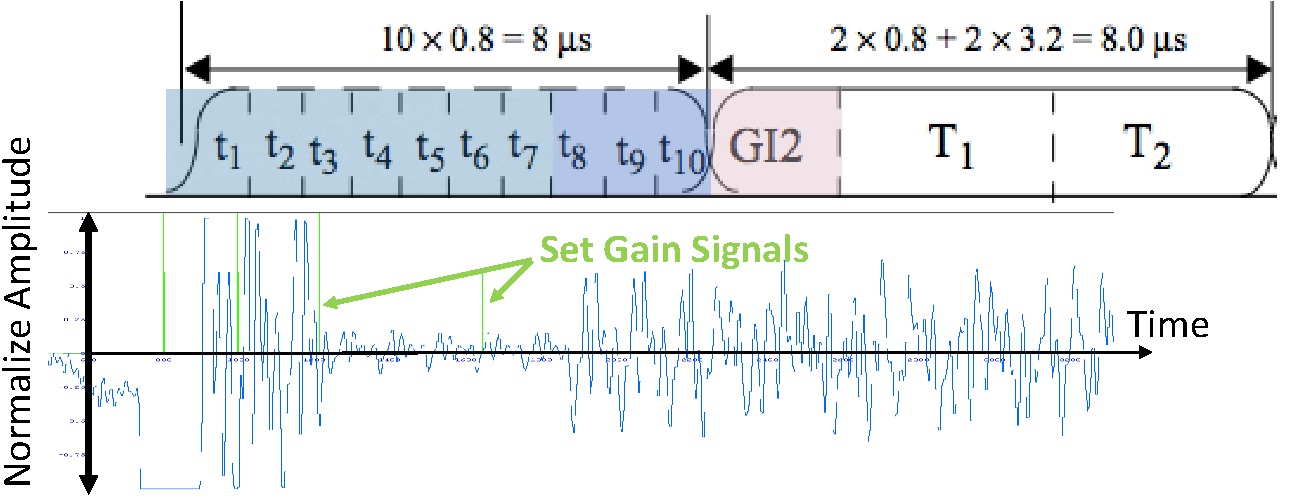
\includegraphics[width=0.9\linewidth]{figs/agc/agc_timing_validation}   
    \caption{Worst-case AGC timing convergence on WURC hardware platform.}
\label{fig_agc_convergence}
\end{figure}
	
\subsection{State Machine Timing Analysis}
\label{sec_agc_timing_analysis}

	In this section, we analyze the timing of the designed system and present recommendations for other system designers to improving timing performance.

	If each saturation detection step take 16 samples and 0.4~$\mu$s at a 40~MHz sampling rate and each round of gain setting takes 0.74~$\mu$s due to the \ac{SPI} bus latency (Section~\ref{sec_agc_timing}), then each coarse gain step takes 1.14~$\mu$s.
	A maximum of three steps takes 3.42~$\mu$s, leaving a remaining 2.18~$\mu$s for packet detection and fine gain control.
	Reliable energy detection of high-SNR signals can be achieved within 16 samples (0.4~$\mu$s), and robust power detection can use any cyclically-shifted version of the 802.11 short training symbols since they are all the same power (0.8~$\mu$s), leaving a small budget of 9 samples (0.225~$\mu$s) for signaling overhead and propagation delays within the digital design.
	
	Unfortunately, in the worst case, when the input signal power is within the purple region in Figure~\ref{fig_agc_coarse_gain}, propagation delay and signaling delays are more than 9 samples, as shown in Figure~\ref{fig_agc_convergence}.
	In this figure, the buffered input \ac{ADC} samples are retrieved from a \ac{WURC} prototype and juxtaposed against the transmitted 802.11 \ac{PLCP} header (top) and the digital gain setting signals (green triggers).
	Three rounds of saturation removal are shown after packet detection (first three green triggers), followed by a long period of fine input power estimation and a final round of gain setting (last green trigger).
	The entire worst-case gain control process is finished within 6.4~$\mu$s, well within the short training preamble, but slightly longer than the 802.11 standards-compliant target of 5.6~$\mu$s.
	
	In each outlined step, decision sample times may be shortened or the logic fine-tuned to reduce the overall worst-case \ac{AGC} convergence time, however it should be clear that the \ac{AGC} timing budget necessitate the use of digital logic as close to the \ac{ADC} as possible.
	
	Luckily, for WARPv3's \ac{OFDM} receiver, the entirety of the 8~$\mu$s short training sequence may be used for \ac{AGC} and fine gain control, thus our system meeting timing requirements for 802.11af-like transmissions utilizing the \ac{WURC} platform.
	Other standards-compliant 802.11 receivers may require that gains must be settled before short training sequence $t_8$, in which case additional optimizations will be required.


%#######################################
\subsubsection{Hardware Controller Architecture}
\label{sec_agc_hw_controller}

	A common design challenge for \ac{SDR} platforms is balancing the desire for flexibility and rapid code development inherent in purely software-based designs with the demand of real-time performance in communications systems.
	We identify a fundamental tradeoff in how the radio physical layer is partitioned: the more abstracted that signal processing becomes from the analog system components, the longer it takes for digital logic to react to events.

\begin{figure}[t] % AGC Design Diagram
\centering
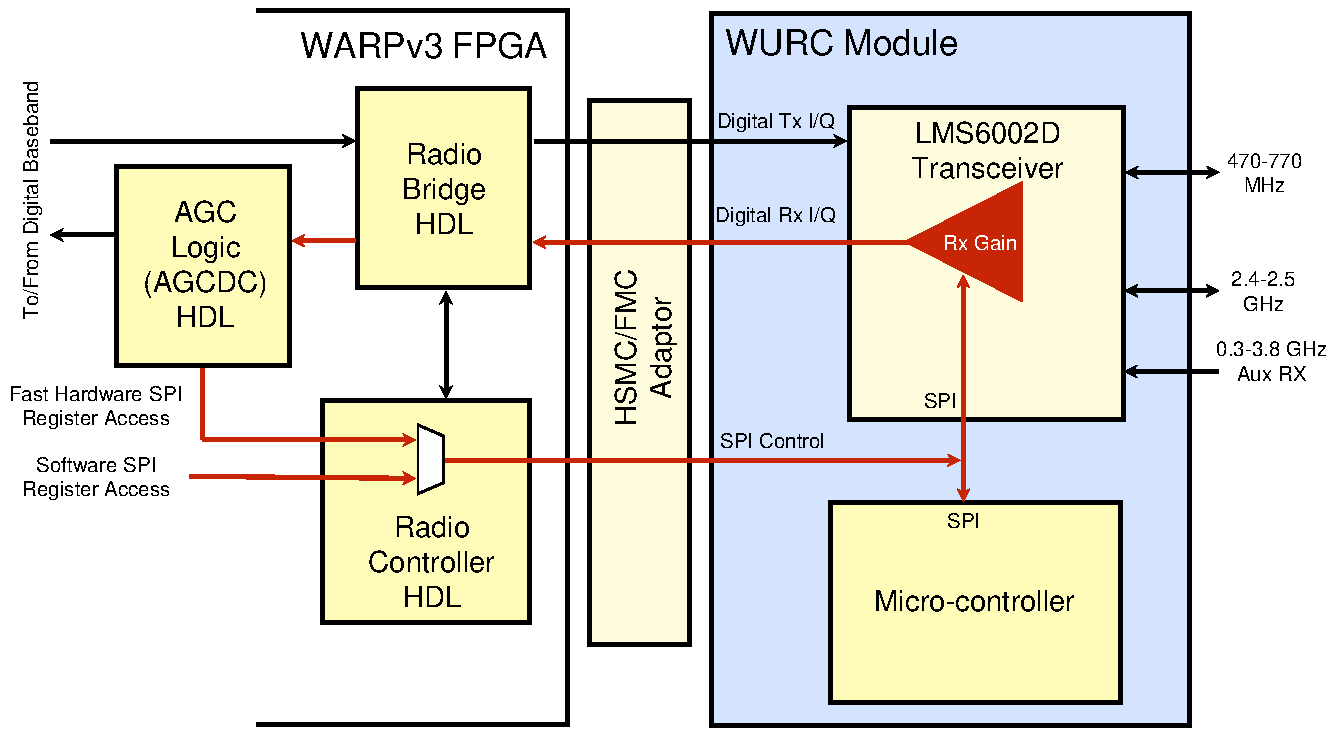
\includegraphics[width=0.9\linewidth]{./figs/agc/agc_block_diagram}
\caption{Hardware control flow of analog AGC design.}
\label{fig_agc_block_diagram}
\end{figure}

	As analog radio transceivers become more integrated and controlled with digital logic, it is important that system designers make architectural decisions that minimize control latencies.
	In order to achieve low-latency operation on \ac{WURC}, we identified time-critical functions such as gain control and embedded their logical functions as close to the digital/analog interface as possible to maximize performance.
	There are four design patterns that are critical to ensuring \ac{SDR} systems can meet high-speed system design demands in \ac{WURC} and other applications:

\begin{enumerate}
\item Direct access to analog control registers from programmable logic or real-time processes enables quick digital reactions,
\item Direct access to analog control registers from software enables cross-layer designs and well-designed software interfaces for complex transceiver configuration options,
\item Register caching in programmable logic avoids lengthy read-modify-write delays when setting analog gains,
\item Control register mappings that consolidate receive gain settings in the smallest number of registers to minimize bus latencies. \label{item_reg_design}
\end{enumerate}

	While we did not have control of Item~\ref{item_reg_design} in this particular system, we observe that transceiver memory maps are increasing in size with complexity and increased programmability and this should be a consideration for future designers of digital transceiver hardware.
	The next-generation LMS7002M utilizes a 16-bit address space with 16-bit depth registers whereas previous generation LMS6002D had an 8-bit address space and 8-bit register depth \cite{lime2012lms6002d, lime2018lms7002M}.
	AD9361 devices use a ``$11+5$'' bit address space and 8-bit register depth.
	However, \ac{SPI} control interfaces remain low-speed for ease of implementation\footnote{\ac{SPI} interface speeds above 50~MHz start to require more advanced design techniques such as length matching, differential signaling, skew and impedance compensation, and provide less safety margin for process variation.}, thus resulting in more time to issue commands to next-generation transceivers.

	The remaining design patterns were implemented with a locally-cached bus arbiter that enabled multi-master direct register access to the LMS6002D transceiver from \textbf{both} high-layer software as well as low-layer programmable logic.
	This new architecture was \emph{required} in order to meet 802.11 standard timing in the \ac{WURC} design without introducing additional analog hardware components as discussed in Section~\ref{sec_agc_related}.
	The multi-master control interface is shown in Figure~\ref{fig_agc_block_diagram}, where both hardware and software \ac{SPI} masters share control over the transceiver \ac{SPI} control bus and arbitration between the masters is implemented in the Radio Controller IP block.
	In addition to performing bus arbitration, the Radio Controller locally caches gain register values so that redundant \ac{SPI} transactions are avoided, eliminating read-modify-write operations in a way that is transparent to the multiple \ac{SPI} masters.
	
	The presented \ac{AGC} logic blocks are available open-source for use in other projects \cite{guerra2012pcores}.
	While some implementation details of this logical design are specific the the hardware platform it was implemented on, the design procedure is generalized for all \acp{SDR} architectures with the same general components as those shown in Figure~\ref{fig_sdr_ideal_rx}.
	In fact, this same system design is being ported to platforms with completely different programmable logic (Xilinx Zynq 7000) and transceiver (Lime Microsystems LMS7002M) subsystems, yet the requirements for high-speed automatic analog gain control have not changed.

%##############################################################3
\subsection{AGC System Evaluation}
\label{sec_agc_system_eval}

	In this section, we evaluate the performance of our fast \ac{AGC} design.
	%Specifically, we are interested in seeing if it can converge fast enough to perform real-time gain control under realistic conditions.
	We wish to show that the designed \ac{AGC} system performs consistently and predictably over all channel gains and consistently meets 802.11 timing requirements.
	A drawback of using the \ac{ADC} as the only sensor for estimating input RF power is that these estimates will be unreliable when the input power falls outside the dynamic range of the \ac{ADC}.
	However, we will show that this system is only unreliable in the high-SNR operating regime where the estimation error does not matter for receiver performance.

\begin{figure}[t]
\centering
  \includegraphics[width=0.9\linewidth]{figs/agc/wsd_manual2_05}   
    \caption{Test setup for AGC evaluation; adjustable attenuator not shown.}
		\label{fig_agc_test_setup}
\end{figure}

	The experimental setup will control the wireless channel between two transmitters to be a simple flat fading channel over a cable between two \ac{WURC} nodes with a variable attenuator (Figure~\ref{fig_agc_test_setup}) where we vary the channel path loss with a variable attenuator in 10~dB steps.
	Assuming that the attenuator provides ideal flat negative gain, this setup ensures that the transmit \ac{SNR} remains constant and the only experimental variables are the receive gain settings and therefore the receive-side \ac{SNR} at the \ac{ADC} input.
	By transmitting a 16-QAM modulated signal (802.11af waveform, 20~MHz channel bandwidth), we are able to detect, decode, and estimate the receive \ac{EVM} of the received signal.
	We expect two sources of increased \ac{EVM}: signals at the \ac{ADC} input that are outside the dynamic range of the \ac{ADC} as identified in Section~\ref{sec_adc_dyn_range}, and decreased \ac{SNR} at the \ac{ADC} input due to weak input power at the antenna port.
	
	With this setup, we program our \ac{AGC} system to target various \ac{ADC} input powers and then transmit 50 802.11af 20~MHz packets constructed in MATLAB using the packet generation framework we built in Section~\ref{sec_static_beamforming}.
		The received packet without \ac{FEC} is decoded and its received \ac{EVM} is calculated as the mean across subcarriers and OFDM symbols of the normalized distance between the received decoded symbol and the intended decoded symbol.

	This experiment is repeated for each target input power between $[-40, 0]$~dBm, with channel attenuation settings between $[60, 100]$~dB in 10~dB steps.
	Figure \ref{fig_agc_rxgain} depicts the performance of the implemented power estimator and \ac{AGC} subsystem design by reporting the mean static receive gain setting that the \ac{AGC} subsystem selected for that packet.
	Error bars in Figure~\ref{fig_agc_rxgain} display the standard deviation across the 50 trials, showing consistent packet detection and input power estimation for all channel attenuation greater than 60~dB.
	At 60~dB, the input power to the \ac{ADC} is so strong that even with all receive gains backed off, the input is still saturated, resulting in inaccurate power estimation and therefore wide variance across selected receive gains for the same input power.
	However, when we look at the receiver \ac{EVM}, we will see that this input gain variance in high input \ac{SNR} conditions is irrelevant to receiver performance.


% AGC RxGain Evaluation
\begin{figure}[ht]
\centering
  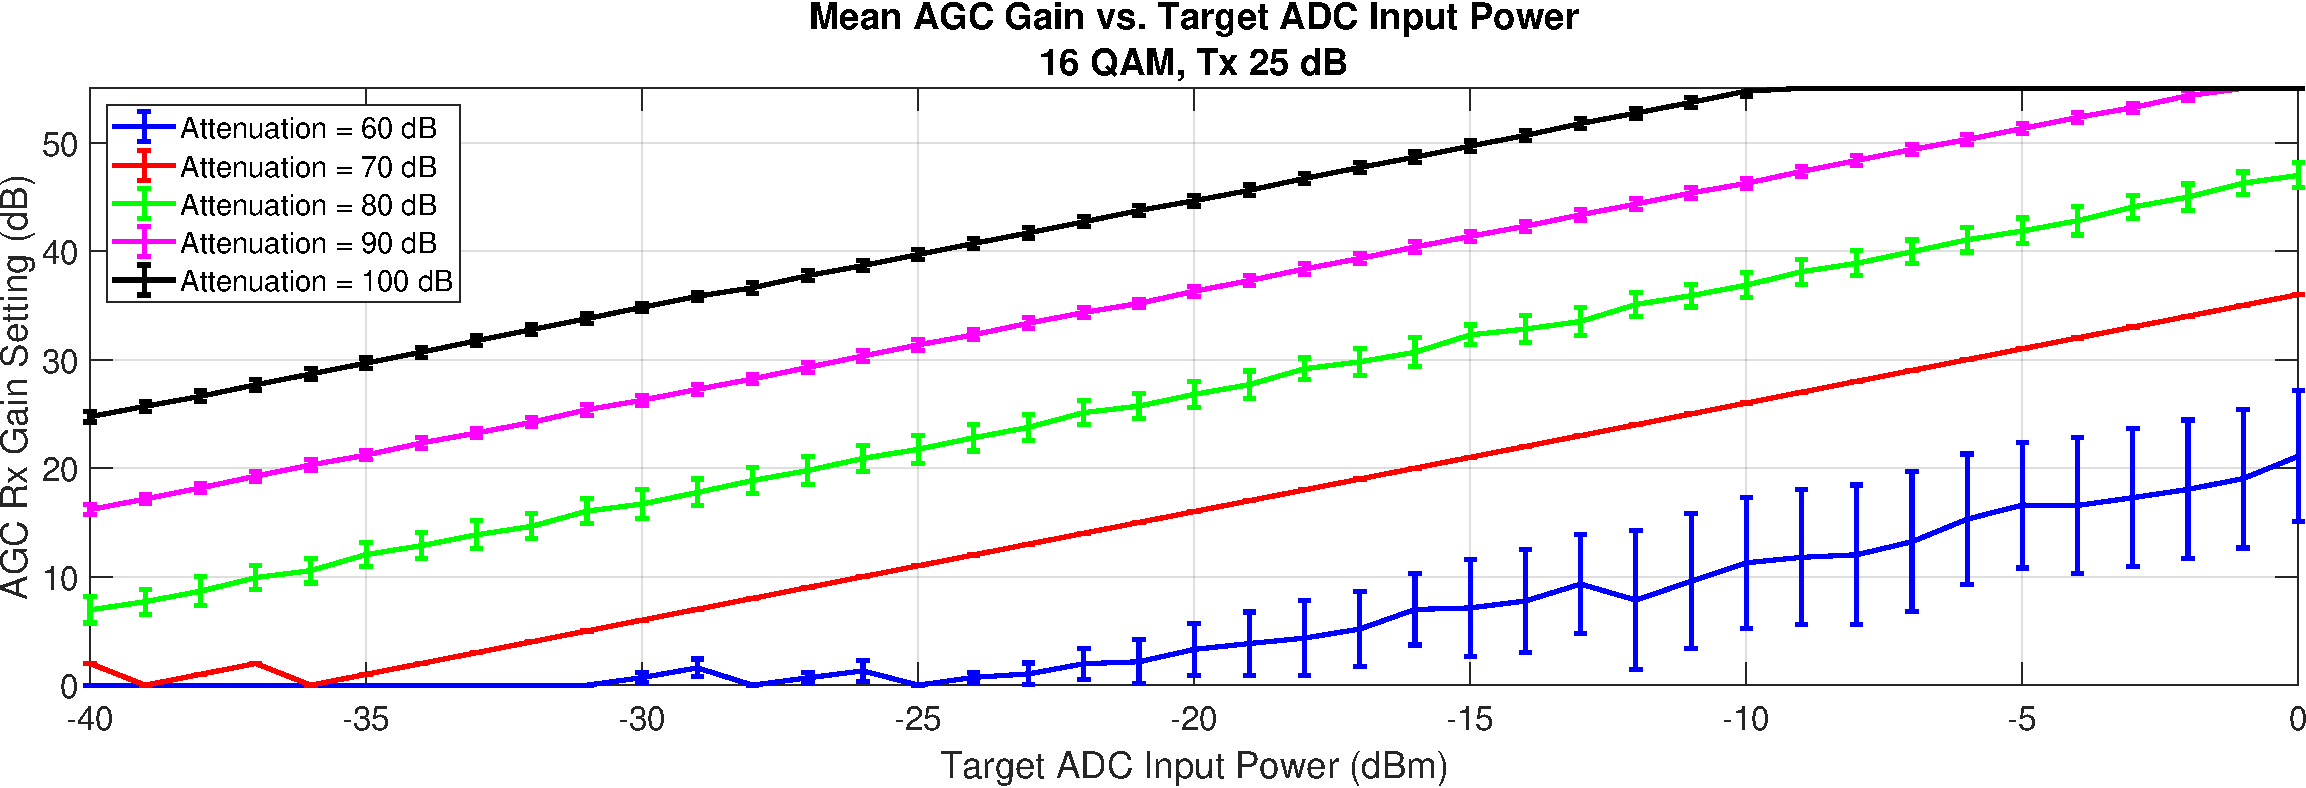
\includegraphics[width=1\linewidth]{figs/agc/AGCTarget_v_EVM_16QAM_ALLdBAtten_Tx25_20MHz_rxgain}   
    \caption{AGC-controlled receive gain setting as a function of ADC input power setting for various channel attenuation and fixed transmit power. Error bars indicate standard deviation across trials.}
\label{fig_agc_rxgain}
\end{figure}
	
	Figure~\ref{fig_agc_evm} shows the measured receive \ac{EVM} for the same set of trials.
	For each attenuation value, the bowl of the EVM curve represents the lower bound on the system's 16-QAM receive EVM, and we have drawn a green shaded region to indicate the target \ac{ADC} input power range that achieves this minimum \ac{EVM} for all input power levels with this 16-QAM modulation.
	The right-most bound of this range is limited by saturation at the ADC and the left-most bound is determined by the system noise floor and quantization error.
	
	% AGC EVM Evaluation
\begin{figure}[hb]
\centering
  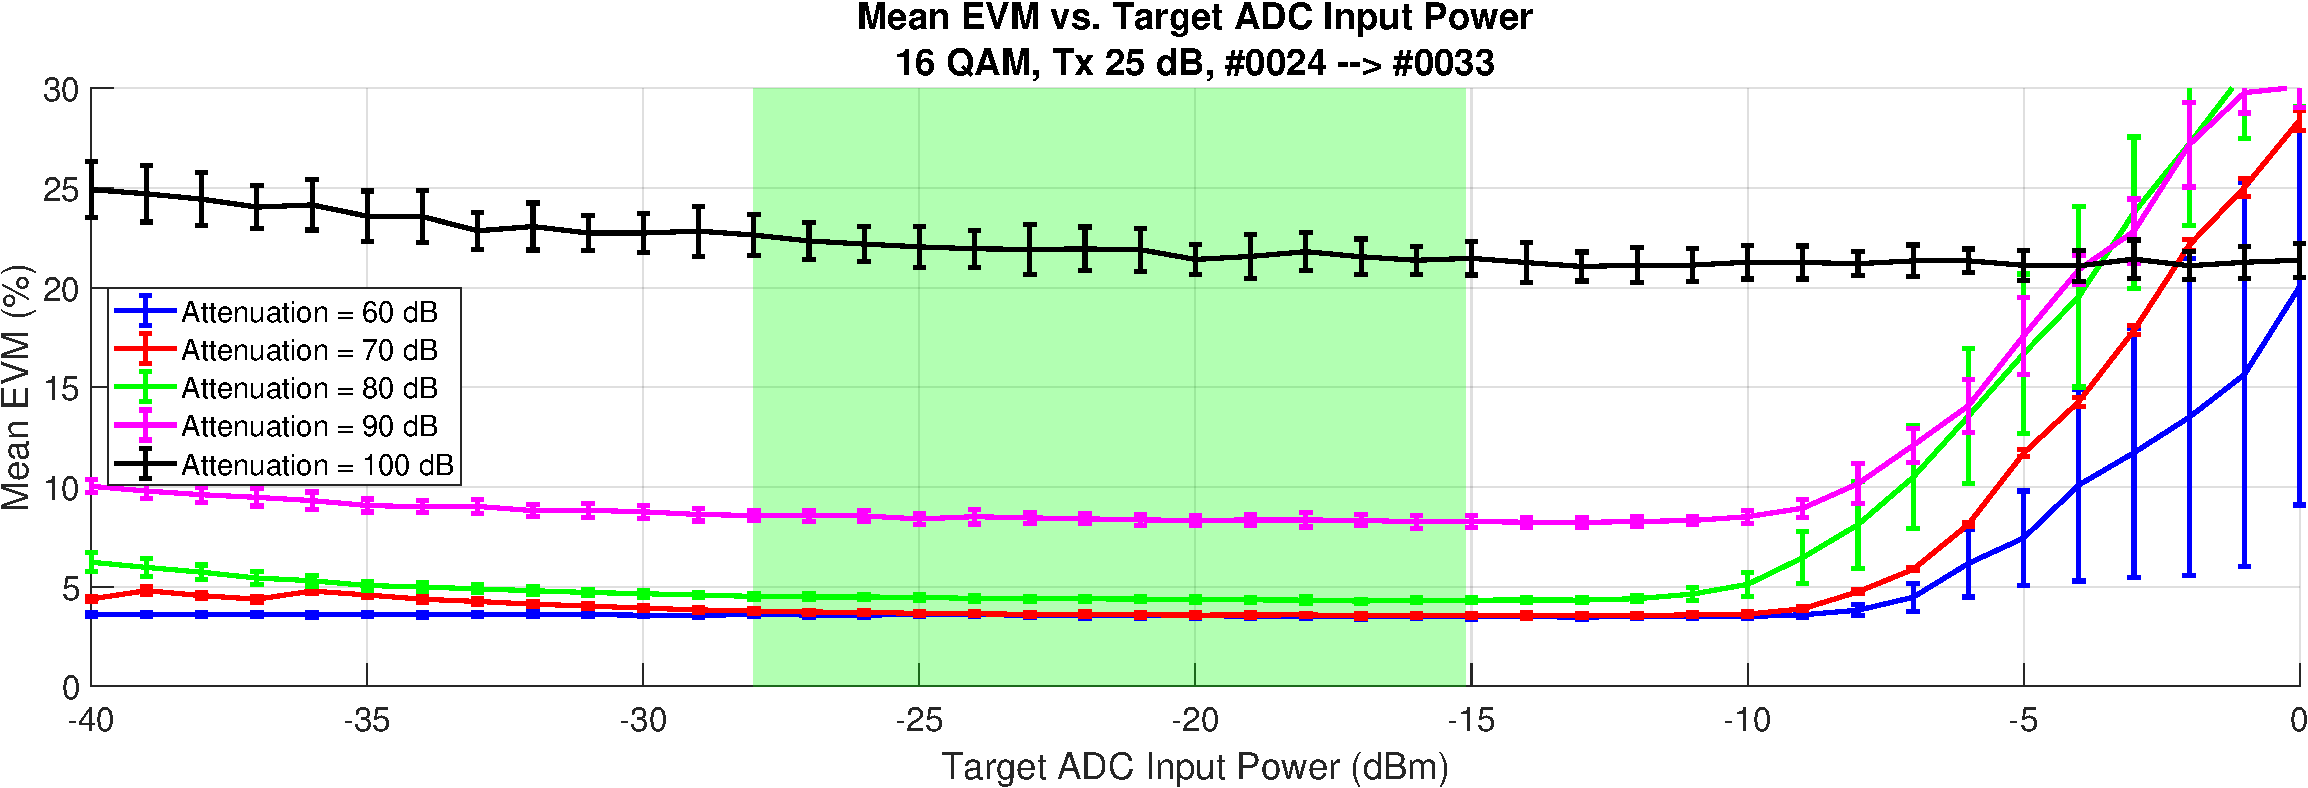
\includegraphics[width=1\linewidth]{figs/agc/AGCTarget_v_EVM_16QAM_ALLdBAtten_Tx25_20MHz_evm}   
    \caption{Received 16-QAM \ac{EVM} as a function of \ac{ADC} input power setting for various channel attenuation. Error bars indicate standard deviation across trials.}
\label{fig_agc_evm}
\end{figure}
	
	To provide some intuition regarding these \ac{EVM} curves, 4\% is the maximum allowed \emph{transmit} \ac{EVM} for an 802.11n transmitter using 64-QAM with $\frac{5}{6}$ coding; 10\% is the maximum allowed transmit \ac{EVM} for 16-QAM with $\frac{5}{6}$ coding; and 2\% is what is required for a 256-QAM transmitter with $\frac{5}{6}$ coding.
	Therefore, although the experiment only used 16-QAM, our implemented system can support the maximum 802.11n modulation rate.
	
	As the channel attenuation increases beyond 70~dB, we see that the achievable minimum \ac{EVM} becomes limited by the signal \ac{SNR} at the \ac{ADC}.
	This effect is particularly obvious at the limits of our testbed at 100~dB channel attenuation, where the mean input power can be reliability estimated as evidenced by the small variance in Figure~\ref{fig_agc_rxgain}, but the receive \ac{SNR} is high and \ac{EVM} becomes dominated by channel and receiver noise in Figure~\ref{fig_agc_evm}.
	
	Based on this evaluation, we fix our target ADC input power to -18 dBm in order to ensure that all received packets are detected and received with minimal quantization error and without clipping.
	This is particular important for the channel measurement studies in Chapter~\ref{sec_environment_chapter}, where channel phase and magnitude estimation accuracy will be important.
	
	Finally, we return to the observation that when the channel attenuation is only 60~dB, saturation causes the \ac{AGC} subsystem to estimate the input signal power inaccurately and select a wide range of receive gain settings for the same input power.
	For the same 60~dB conditions in Figure~\ref{fig_agc_evm}, we can see there is no impact on the \ac{EVM} performance at all in this regime.
	



%##############################################################3
\subsection{Conclusion and Discussion}
\label{sec_agc_conclusion}


	In this section, we have presented the design of an \acf{AGC} system designed for generic \ac{SDR} hardware that does not require the use of external power estimation components.
	We implemented this design on our custom \ac{TVWS} \ac{SDR}, integrating it with the WARPv3 \ac{SDR} platform to construct the first real-time 802.11af-like system with full dynamic range of operation.
	
	A key observation is that the \ac{SPI} control bus between programmable logic and the analog transceiver is the largest arbitrary timing bottleneck, limiting the speed at which we can control receive gains.
	Poor digital design of transceiver register maps has resulted in the need to execute multiple \ac{SPI} bus transactions to change receive gains when fundamentally these settings could be located in a single control register.
	Our recommendation for the design of future \ac{SDR} platforms is to aggregate the digital receiver gain settings in a single control register on the transceiver, making similar \ac{AGC} systems respond more quickly and able to meet even more challenging timing constraints.
	
		While not all \ac{SDR} platforms will be able to use our \ac{AGC} design as-is, we have taken care to present the design motivations and implementation steps such that the same design steps can be applied to other platforms.
	In particular, we discussed the timing limitations required to implement our design in Section~\ref{sec_agc_timing_analysis}; it is clear that \acp{FPGA} or similar programmable digital logic that operates at a high clock speed is required to implement our system and hope to meet very tight 802.11 timing requirements.
	Should another \ac{SDR} platform meet these requirements, then the digital logic blocks we have released open-source \cite{guerra2012pcores} and design procedures we have presented here will allow them to realize the entire dynamic range of their receiver front-end without additional analog hardware components.


	%	\section{Physical Layer Calibration for SDR Systems}
		\subsection{System Architectures}
			\rgnote{Present the architecural diagram of a direct-conversion transceiver and where analog impairments give rise to distortion in the signal path. I may just cut this section if time goes short. It's critical hardware development and involved testing of which parts were process or temperature variant, but it also requires a lot of detailed diagrams and explanation that is probably not worth it. Practically, this kind of discussion and information is VERY useful to other system designers and I wish I'd had a thesis-level discussion regarding this material rather than having to figure it out via lengthy trial and error.}
		\subsection{Calibration Algorithm Design}
			\rgnote{TODO: expand beyond the brief.}
			Based on our observations of calibration behavior, we designed a non-volatile database approach to IQ imbalance correction to shorten calibration time and complexity, allowing us to avoid the inclusion of dedicated analog feedback paths in the hardware design.
			However, \ac{LOFT} calibration varied with time, temperature, and center frequency, requiring on-demand calibration.
			Therefore, we designed the software driver framework to support on-demand calibration of LOFT components when setting center frequencies and validated our calibration libraries with direct measurement and over-the-air testing.
	%###############################################
%\section{Fast Tx/Rx Switching Design for 802.11 TDD Support}
%%\label{wurc_tdd_switching}
%
%\rgnote{Discussion on the design, implementation, and testing of the 5~us Tx/Rx switching necessary to support 802.11 on WURC. This is also a section that may get cut in the interest of time or there not being sufficient research contribution vs. engineering documentation.}
%
%
%\begin{figure}[t]
%\centering
 %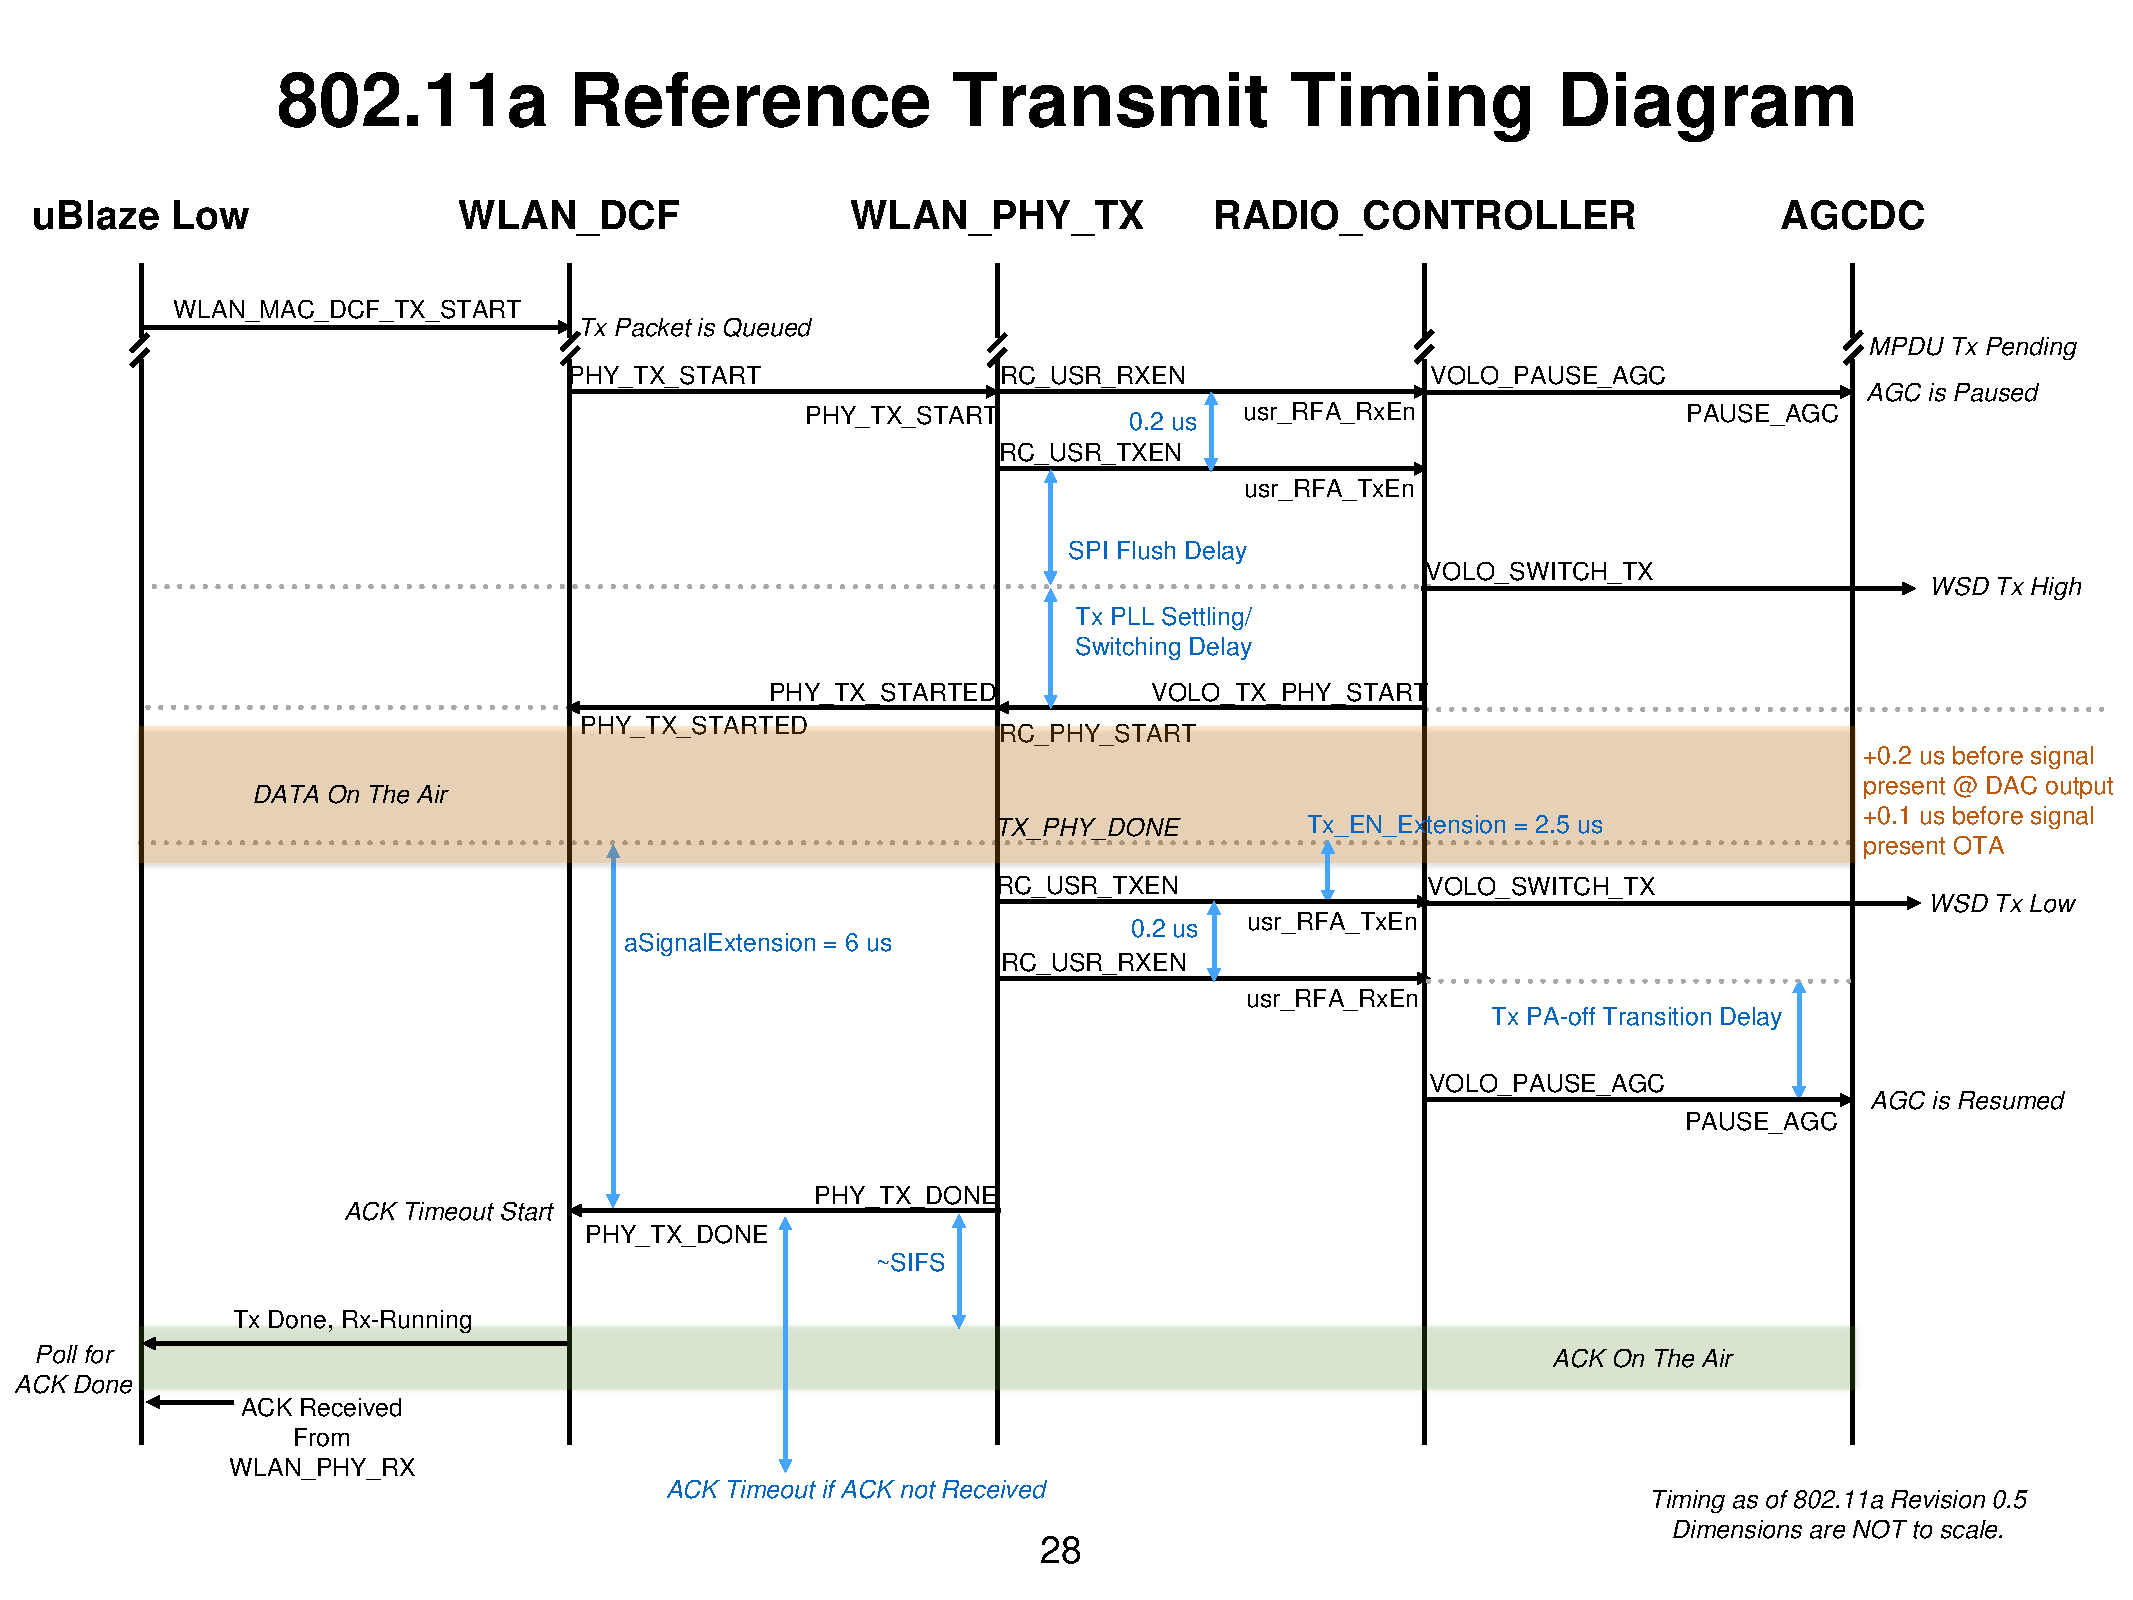
\includegraphics[width=0.9\linewidth]{figs/wurc/wurc_80211_timing_reference}   
    %\caption{Timing diagram for calibrating PHY hardware delays. \rgnote{TODO: write up this section regarding fast 802.11 Tx/Rx switching and its impact on performance} }
%\label{fig_wurc_timing}
%\end{figure}



%%###############################################
 \section{WURC Software Architecture}
\label{sec_wurc_sw_arch}

	As a software-defined radio system, the real-time software architecture of the \ac{WURC} platform represented a significant design challenge spanning high-level software architecture and low-level \ac{HDL} development.
	First, \ac{WURC} was designed as a modular, scalable system, and we desired to compartmentalize as many functions as possible while still retaining cross-layer access and control.
	Second, we wished to utilize existing \ac{PHY} prototyping frameworks such as WARPLab \cite{warplab} and the 802.11 Reference Design \cite{warp80211} from the \ac{WARP} project to provide starting points for implementing our \ac{MU-MIMO} testbed and 802.11af platform, respectively.

	To that effect, we designed a platform with an embedded micro-controller, the Texas Instruments Stellaris LM3S5R36 \cite{ti2012stellaris}, that would serve as a controller and abstraction layer for the agile software-defined radio transceiver, Lime Microsystems LMS6002D, and present high-level radio control functions to the host system.
	The software libraries embedded within the micro-controller were designed to be self-contained and portable, thus allowing a host system to integrate \ac{WURC} with minimal changes to the platform code, and to port this driver library to other hardware architectures easily.
	In this section, we present the software and firmware architectures for the WURC-based platformed presented in this thesis.

% WURC 802.11 Software/Firmware Architecture
\begin{figure}[p]
	\centering
  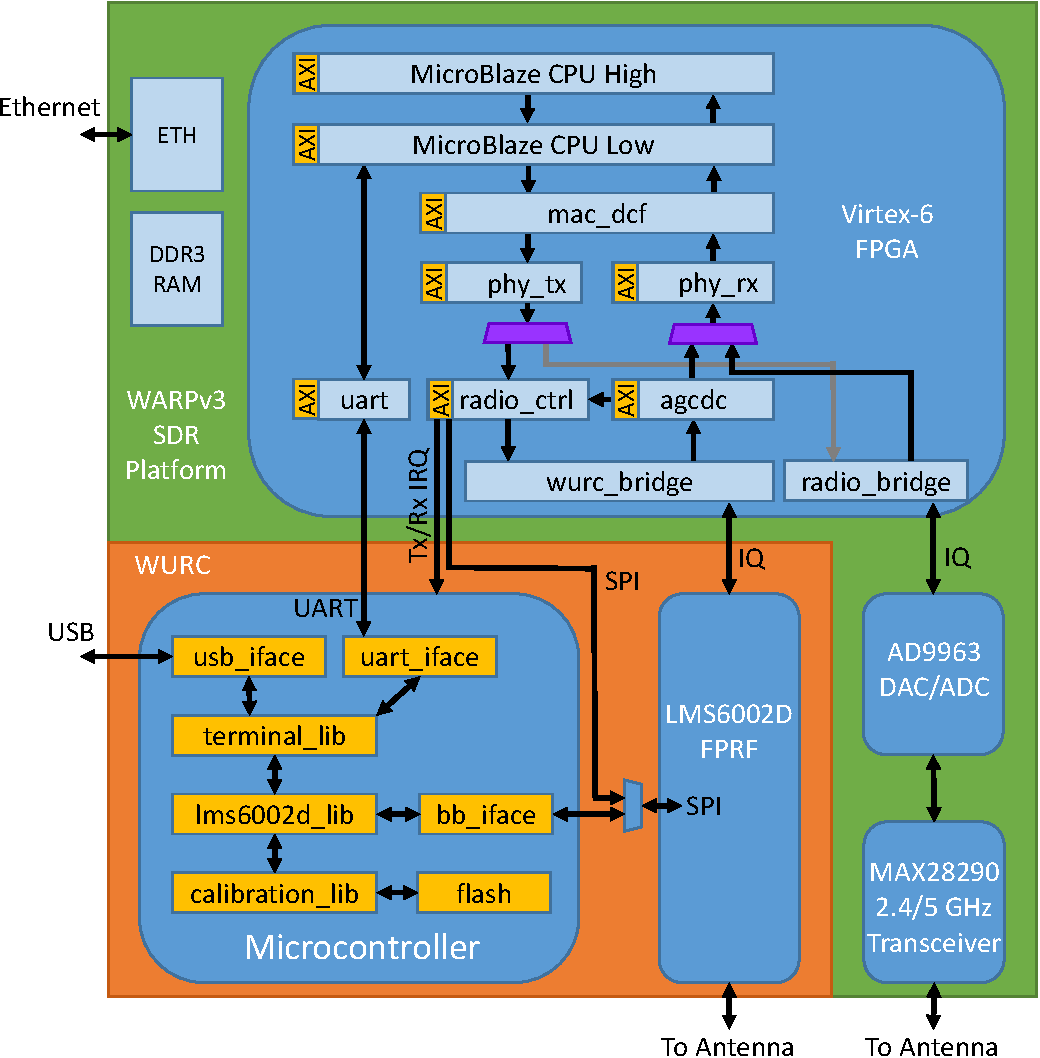
\includegraphics[width=1\linewidth]{figs/wurc/wurc_80211_hdl_design}   
  \caption{Software and HDL architecture of WURC/WARPv3 802.11 design.}
	\label{fig_wurc_80211_arch}
\end{figure}
	
% LMS6002D Library
\subsection{Agile \ac{SDR} Transceiver Driver \texttt{lms6002d\_lib}}
\label{sec_wurc_lms_lib}

	We designed and tested a platform-agnostic open-source C library of general calibration and configuration functions tailored for the LMS6002D agile RF transceiver \cite{guerra2013lms6002d}.
	The general architectural design and major interfaces between components is presented in Figure~\ref{fig_wurc_80211_arch}.
	The \ac{WARP} hardware components are contained within the green part of the system diagram while the \ac{WURC} hardware components are encapsulated within the red part (matching the color scheme in Figure~\ref{fig_warp_wurc_hw}; \ac{FPGA} code blocks for new \texttt{radio\_ctrl}, \texttt{agcdc}, and the \texttt{wurc\_bridge} modules were also developed.
	Aside from extremely time-sensitive operations such as receive gain control, all communications to the transceiver are filtered through a driver library \texttt{lms6002d\_lib} executing on a microcontroller embedded on each \ac{WURC} board.
	
	This encapsulation is necessary since the amount of parameter tuning, calibration, and self-test necessary to support basic analog transceiver functions grows significantly the more flexible a \ac{SDR} transceiver becomes.
	In application-specific radios, a discrete set of operational modes may be programmed and optimized; a truly agile transceiver must support a continuous range of center frequencies, modes of operation (TDD/FDD), channel bandwidths and analog waveforms, each requiring specific optimization.

	For example, changing the radio center frequency in an agile transceiver requires a complex set of actions: select the appropriate frequency synthesizer, tune synthesizer RC constants for optimal noise performance, load analog calibration values for IQ imbalance compensation, tune anti-aliasing filter RC constants, and calibrate analog component DC levels to remove \ac{LOFT} amongst other actions.
	As a result, many simple radio functions take hundreds of control register interactions with the underlying LMS6002D transceiver; we managed this complexity by encapsulating these actions with high-level functions designed to abstract the analog front-end and enumerated in Appendix~\ref{sec_wurc_console}.

	For large arrays of \ac{WURC} radios, a host can broadcast simple commands to initialize and configure the analog \ac{WURC} baseband via the \ac{UART}, and the on-board microcontrollers will compensate for the state and process variation for each radio while monitoring and reporting faults to the host system.
	
	This design offloaded a very significant amount of complexity and computation from the FPGA host and is one necessary component for scaling the number of radio modules in a large-scale \ac{WURC} array.

% LMS6002D Calibration
\subsubsection{SDR Transceiver Calibration \texttt{calibration\_lib}}
\label{sec_wurc_calibration}

	The calibration library is designed to interact with non-volatile flash memory on each \ac{WURC} device to store and retrieve radio calibration data generated for each \ac{WURC} during manufacturing.
	These analog compensation values are loaded in response to frequency and gain settings for the purpose of compensating for process variation in the LMS6002D direct-conversion transceiver.
		There are two types of analog radio calibration that are dependent on \ac{IC} manufacturing process variation and that we found were persistent for the lifetime of the LMS6002D transceiver.

	The first, \acf{LOFT}, is caused when the RF oscillator couples to the input of the receive mixer such that it mixes with itself down to baseband and appears as a strong tone at the 0th frequency, or DC component.
	This is a well-known impairment that is intrinsic to direct-conversion transceiver architectures and which can be compensated by applying a correction DC offset signal proportional to the strength of the receive \ac{LOFT}.
	We have found this value to be consistent, frequency-dependent, and smooth across the UHF band using \ac{WURC} hardware, therefore we store a series of scalar DC analog voltage correction levels in non-volatile flash memory that are loaded into correction DACs embedded in the LMS6002D receive chain each time the receive frequency is tuned by the driver.
	The goal of the compensation signal is to counter-act the known \ac{LOFT} DC component such that the finite \ac{ADC} dynamic range is not exceeded.
	Once a compensation signal is added to the analog signal, the remaining \ac{LOFT} DC component can be easily removed in the digital domain with a digital low-pass filter.

	The second calibration is for IQ imbalance, which is caused by differences between the I and Q circuit paths within the LMS6002D quadrature transceiver in terms of gain and phase.
	These imbalances result in the generation of image tones on both the input and output signals after quadrature mixing \cite{tubbax2005compensation}.
	Similar to \ac{LOFT}, this impairment is consistent, frequency-dependent, and smooth across the UHF band.
	However, given the digital architecture of our system, these corrections must be applied in the digital domain on the FPGA and are therefore more complex to implement\footnote{Recent generations of agile RF transceivers include these digital correction block on-chip \cite{lime2018lms7002M, adi2018adrv9009}}.
	We calculate optimal phase and magnitude compensation values during manufacture for each 6~MHz UHF channel, then store a triplet of pre-computed coefficients in non-volatile flash memory that will perform the needed vector rotation and gain adjustment on the digital IQ stream.
	These values are loaded to the respective transmit or receive data flow each time the frequency is changed via the UART terminal interface to the host logic.
	
	Since we find the correction values to be smooth functions,\footnote{In fact, a sure indicator of a damaged or malfunctioning \ac{WURC} transceiver is non-smooth calibration coefficients with respect to frequency.} we are able to conserve non-volatile memory space by storing calibration values at several discrete points across our operating frequency range and interpolating calibration values for any arbitrary center frequency between calibration points.
	

% Discussion of the Terminal Interface
\subsubsection{WURC User Control Interface \texttt{terminal\_lib}}
\label{sec_wurc_terminal}

	In order to make the architecture portable and extensible, we separated I/O functions with the \ac{FPRF} transceiver into a separate \texttt{bb\_iface} \ac{API} and user \acp{API} into a custom terminal (\texttt{terminal\_lib}) with the ability to interact through multiple, abstracted character-based interfaces like \ac{USB} (\texttt{usb\_iface}) or \ac{UART} (\texttt{uart\_iface}).
	This makes our designed driver libraries useful for other systems based on the LMS6002D \ac{IC} and readily portable to other CPU architectures.

	The available top-level console commands are described in Appendix~\ref{sec_wurc_console} and can be accessed at any time from either a user connected to the \ac{WURC} terminal directly via \ac{USB}, or from the host via the WARP terminal.

% Tx/Rx Optimization
\subsubsection{Transmit/Receive Switching IRQ Abstraction}
\label{sec_txrx_switching}

For \ac{TDD} protocols like 802.11af, the hardware switching time to turn a radio from transmit to receive or vice-verse is one of the fundamental parameters that drives protocol timing and can be as low as 10~$\mu$s \cite{std11af}.

	This seemingly simple operation encapsulates a number of sequential operations to disable the previously active RF chain and enable the previously inactive chain; on an agile \ac{SDR}, the precise timing of that sequence becomes necessary to manage carefully.
	To this effect, we designed the \ac{WURC} to present a single I/O pin to the host hardware that could be switched high or low while the \ac{WURC} is configured for \ac{TDD} mode to signal the module to shift into transmit or receive mode, respectively.
	Similar to the fast analog gain control design presented in Section~\ref{wurc_agc}, careful analysis and optimization of sequence timing is important to meet timing deadlines.

	We designed the single-pin abstraction to provide a simple Tx/Rx interface to the host that would trigger an interrupt-driven subroutine within the Stellaris microcontroller.
	Figure~\ref{fig_wurc_80211_arch} shows the ``Tx/RX IRQ'' line directly connecting the radio controller to a Stellaris interrupt pin.
	In order to meet timing requirements, it was necessary to flatten the interrupt functional structure and hand-optimize serial command writes and GPIO signals in assembly code in order to enable/disable amplifiers in a precisely timed sequence.
	Combined with tuning of the \ac{WURC} amplifier noise-immunity RC constants and the LMS6002D's frequency synthesizer settling times, we were able to achieve a Tx/Rx turnaround time less than 5~$\mu$s, providing sufficient margin for the MAC layer to make decisions.
	
	%This same logical interface, allowing a host to simplify Tx/Rx switching while pushing real-time control of radio hardware to separate embedded logic, is a key design concept in more recent \acp{SDR} platforms.


%% Discussion of the 802.11 Integration 
%\subsection{WARP 802.11 Integration}
%\label{sec_wurc_80211}
%
	%We integrated the \ac{WURC} \ac{SDR} radio platform with the WARP platform as shown in Figure~\ref{fig_wurc_80211_arch}.
%\rgnote{I couldn't think of anything not engineering to put here. So cut.}

% Discussion of the WARPLab Integration
\subsection{WARPLab Integration}
\label{sec_warplab}

	The WARPLab framework from Mango Communications is an open-source experimental framework that enables a host to synchronize an arbitrarily large number of WARPv3 hosts connected via a Layer 3 backhaul network to perform non-realtime over-the-air experiments \cite{warplab} using MATLAB as a signal processing and coordination environment.
	When a subset of those WARPv3 radios physically share their RF reference clocks and timing reference triggers, the over-the-air transmissions can be made coherent.
	
	WARPLab operates by utilizing MATLAB scripts to generate transmit sample buffers for arbitrary topologies of coherent radio arrays and individual radio nodes with arbitrary baseband signals.
	Once pre-loaded across the experimental topology, a synchronized and hardware-accelerated ethernet trigger\footnote{Handling of the received ethernet trigger on WARPv3 node is performed in \ac{FPGA} hardware, avoiding non-deterministic network stack processing latency.} packet is sent to all nodes, causing them all to simultaneously transmit and/or receive on their radios as pre-configured.
	The receive waveforms are stored in a local receive sample buffer for retrieval.
	A layer 2 communications framework built on MATLAB allows rapid distribution of transmit samples buffers and retrieval of receive sample buffers for post-processing. 
	Of particular importance for enabling conherent \ac{MIMO} transmissions, an array of coherent WARPv3 nodes sharing an RF reference clock does not simply use the ethernet trigger packet for timing synchronization as that would introduce non-deterministic transport delays between nodes.
	Rather, they designate a master node that distributes a simultaneous \ac{GPIO} trigger signal to all slave WARPv3 nodes in order to ensure sample-level synchronization of the coherent radios.
	More details are provided within the WARP project documentation \cite{warplab}.
	
	In Appendix~\ref{sec_warplab_arch}, we present a mapping of WARPLab's functional architecture and highlight parts of the MATLAB code base where we were able to extend WARPLab functionality to transparently support \ac{WURC} transceivers in addition to the built-in WARPv3 transceivers.
	This enabled WARPLab-based experiments to be performed in \ac{TVWS} bands.
	
% WARPLab timing analysis
\subsubsection{WARPLab Latency Analysis}
\label{sec_warplab_timing}

	WARPLab 7 contains a number of transport improvements that result in the ability to perform near-real-time experiments by rapidly performing cycles of: precompute, load, transmit/receive, fetch, and process on the order of 2.5~ms.
	A fast central coordinator using jumbo ethernet frames for transporting IQ buffers and a compiled MATLAB-mex transport layer can operate at per-packet time intervals by decreasing both ethernet transport overhead and network stack latency.
	We observed that extra switches between WARPLab nodes produce measurable switching delay and recommend the use of long ethernet cables and minimization of the number of ethernet hops for WARPLab backhaul.

	While WARPLab is a powerful \ac{PHY} prototyping tool, the two largest drawbacks of WARPLab is that it: 1) requires a central coordinator connected via gigabit ethernet switches; and 2) real-time protocol implementations generally require processing at microsecond symbol-level timescales whereas WARPLab performs centralized signal processing on millisecond packet-level timescales.
	These two factors hinder long-distance or mobile experiments where the installation of a wired ethernet backhaul is quite difficult or nodes move too rapidly to make protocol decisions using WARPLab's centralized framework.
	
	%\rgnote{Put the WARPLab 4x1 HDL architecture diagram here}
	
%\subsubsection{WARPLab Example Application: Spectrum Scanner}
%\label{sec_scanner_app}
%
%
%
%\begin{figure}[p]
	%\centering
  %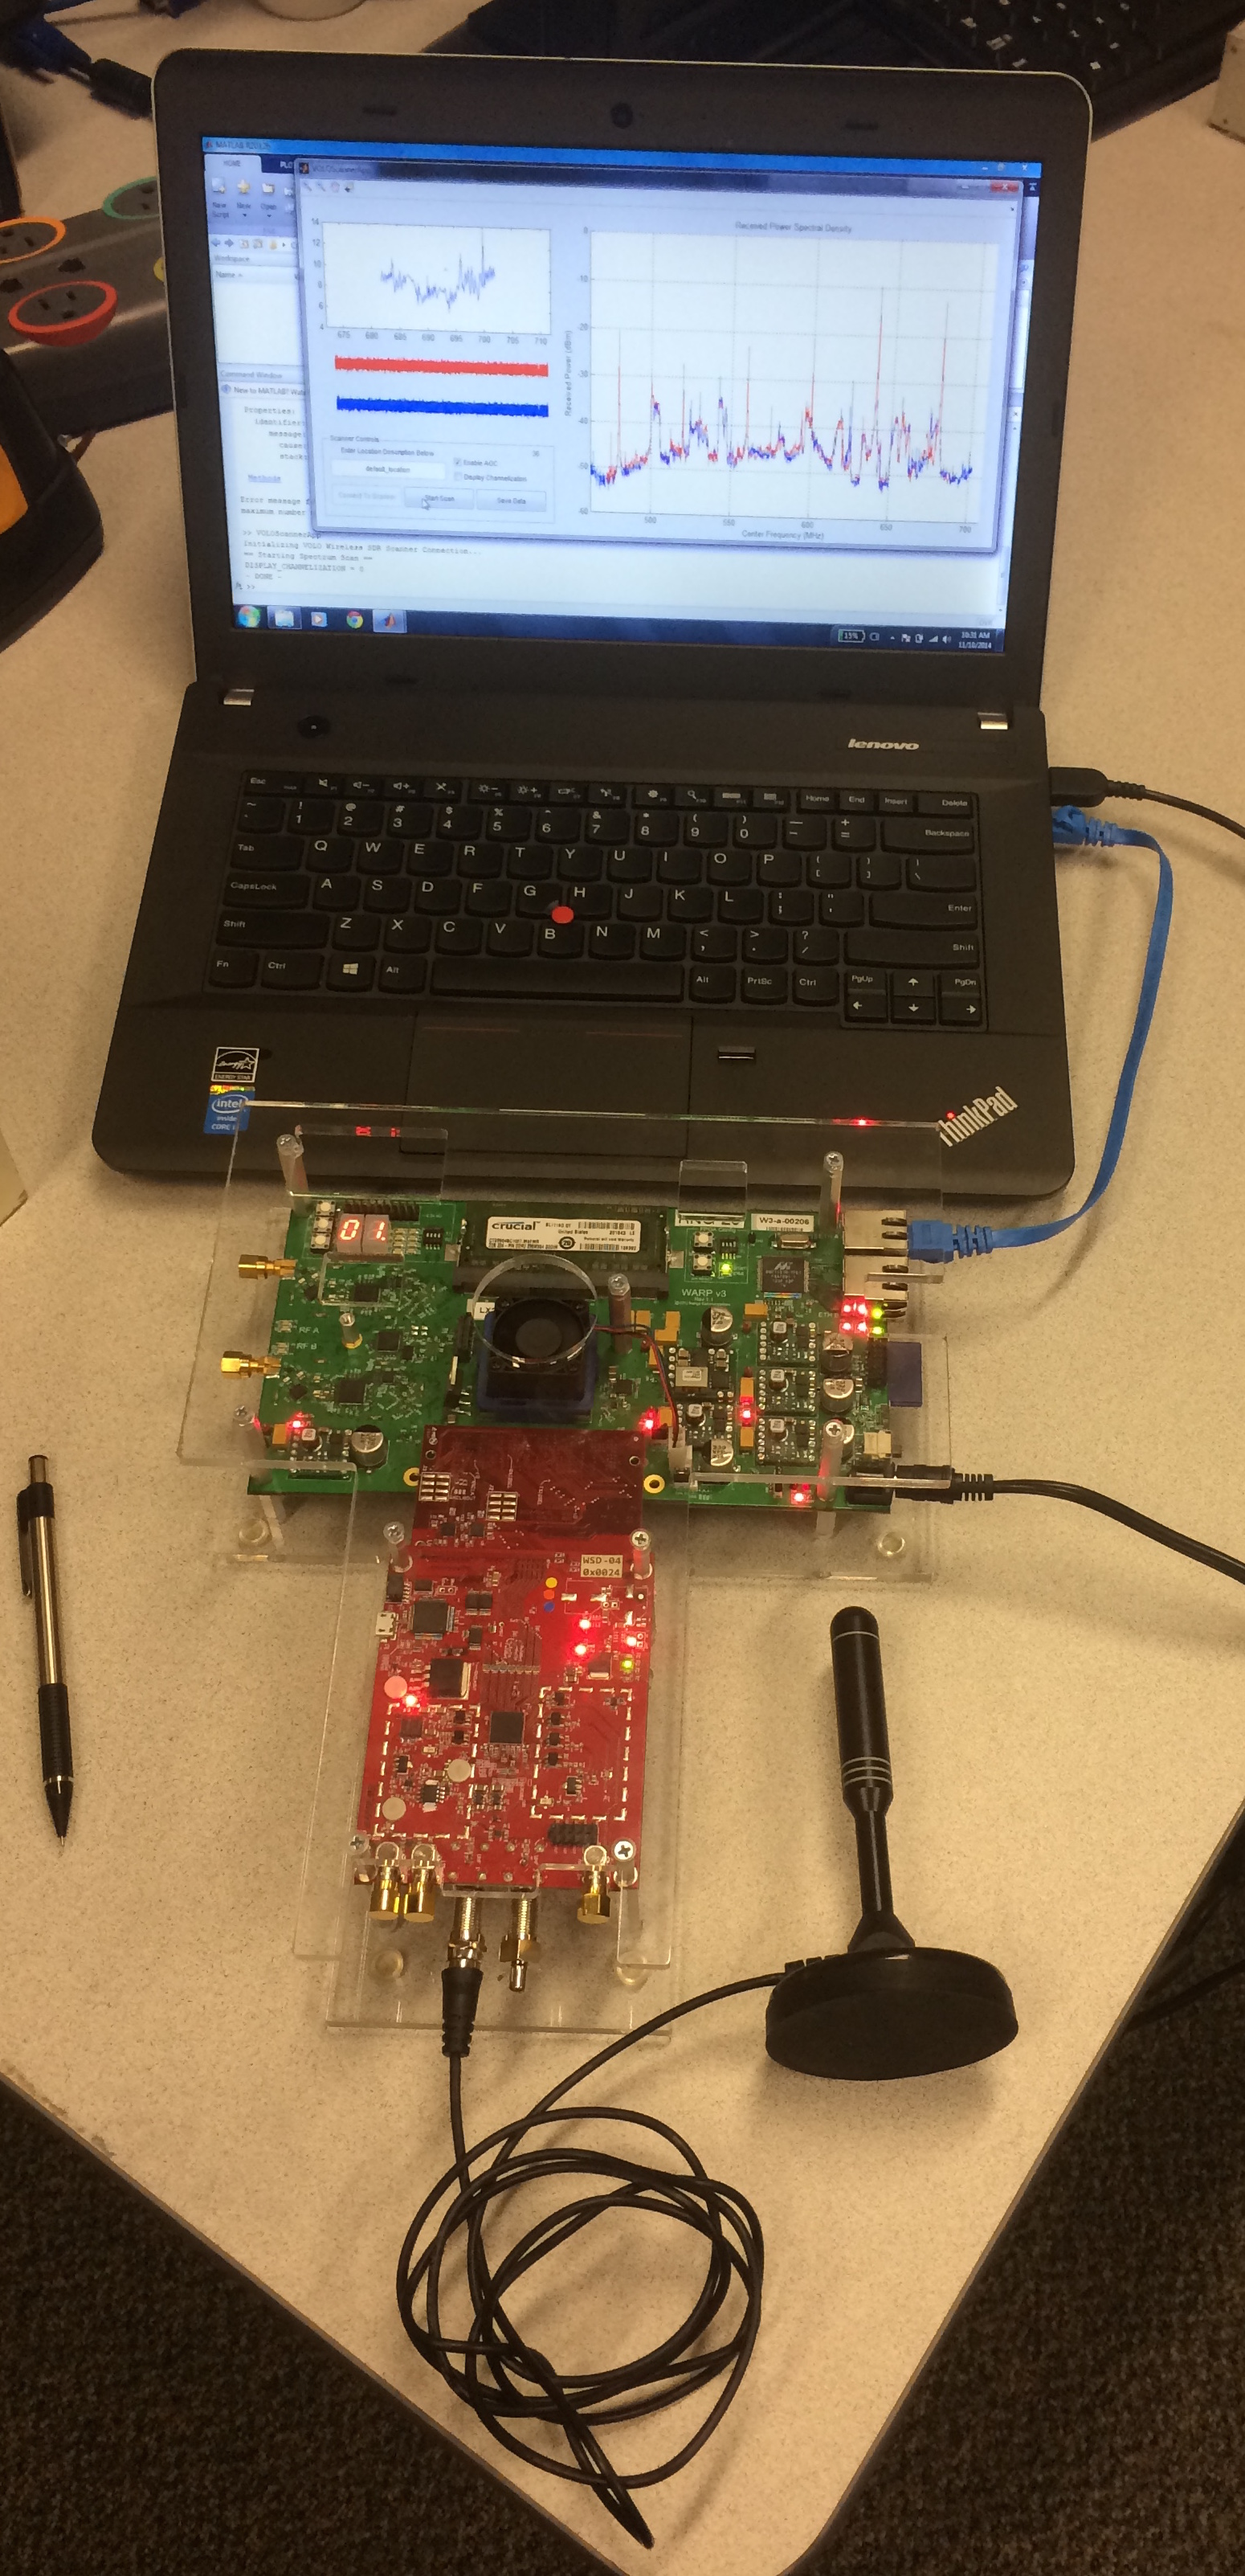
\includegraphics[width=0.4\linewidth]{figs/wurc/scanner_hw}   
  %\caption{Hardware setup for WURC Spectrum Scanner application.}
	%\label{fig_wurc_scanner_hw}
%\end{figure}
%
%\begin{figure}[p]
	%\centering
  %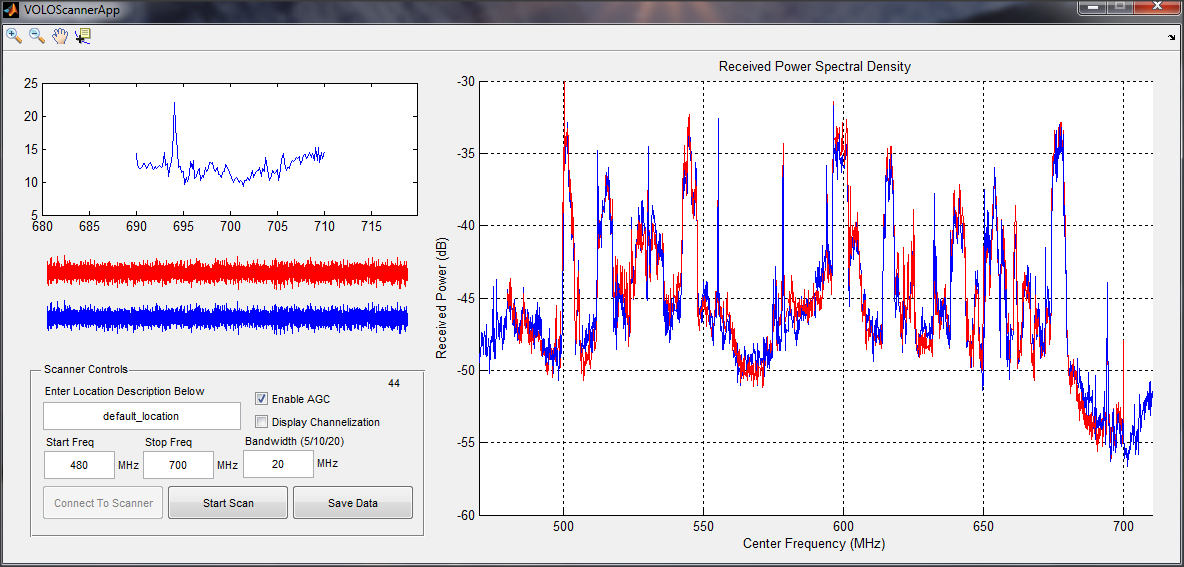
\includegraphics[width=0.8\linewidth]{figs/wurc/scanner_run_indoor}   
  %\caption{GUI for WURC Spectrum Scanner application.}
	%\label{fig_wurc_scanner_gui}
%\end{figure}



	\section{WURC Array 4x4}
\label{sec_wurc_4x4}

	Building upon the single-radio \ac{WURC} module developed in Section~\ref{sec_wurc_module}, we constructed a 4x4 \ac{MU-MIMO} testbed using the WARPv3 platform augmented with the \ac{WURC} UHF-band \ac{SDR} modules (Figure~\ref{fig_wurc_4x4_testbed}).
	
	
% WURC 4x4 Testbed system diagram
\begin{figure}[p] 
\centering
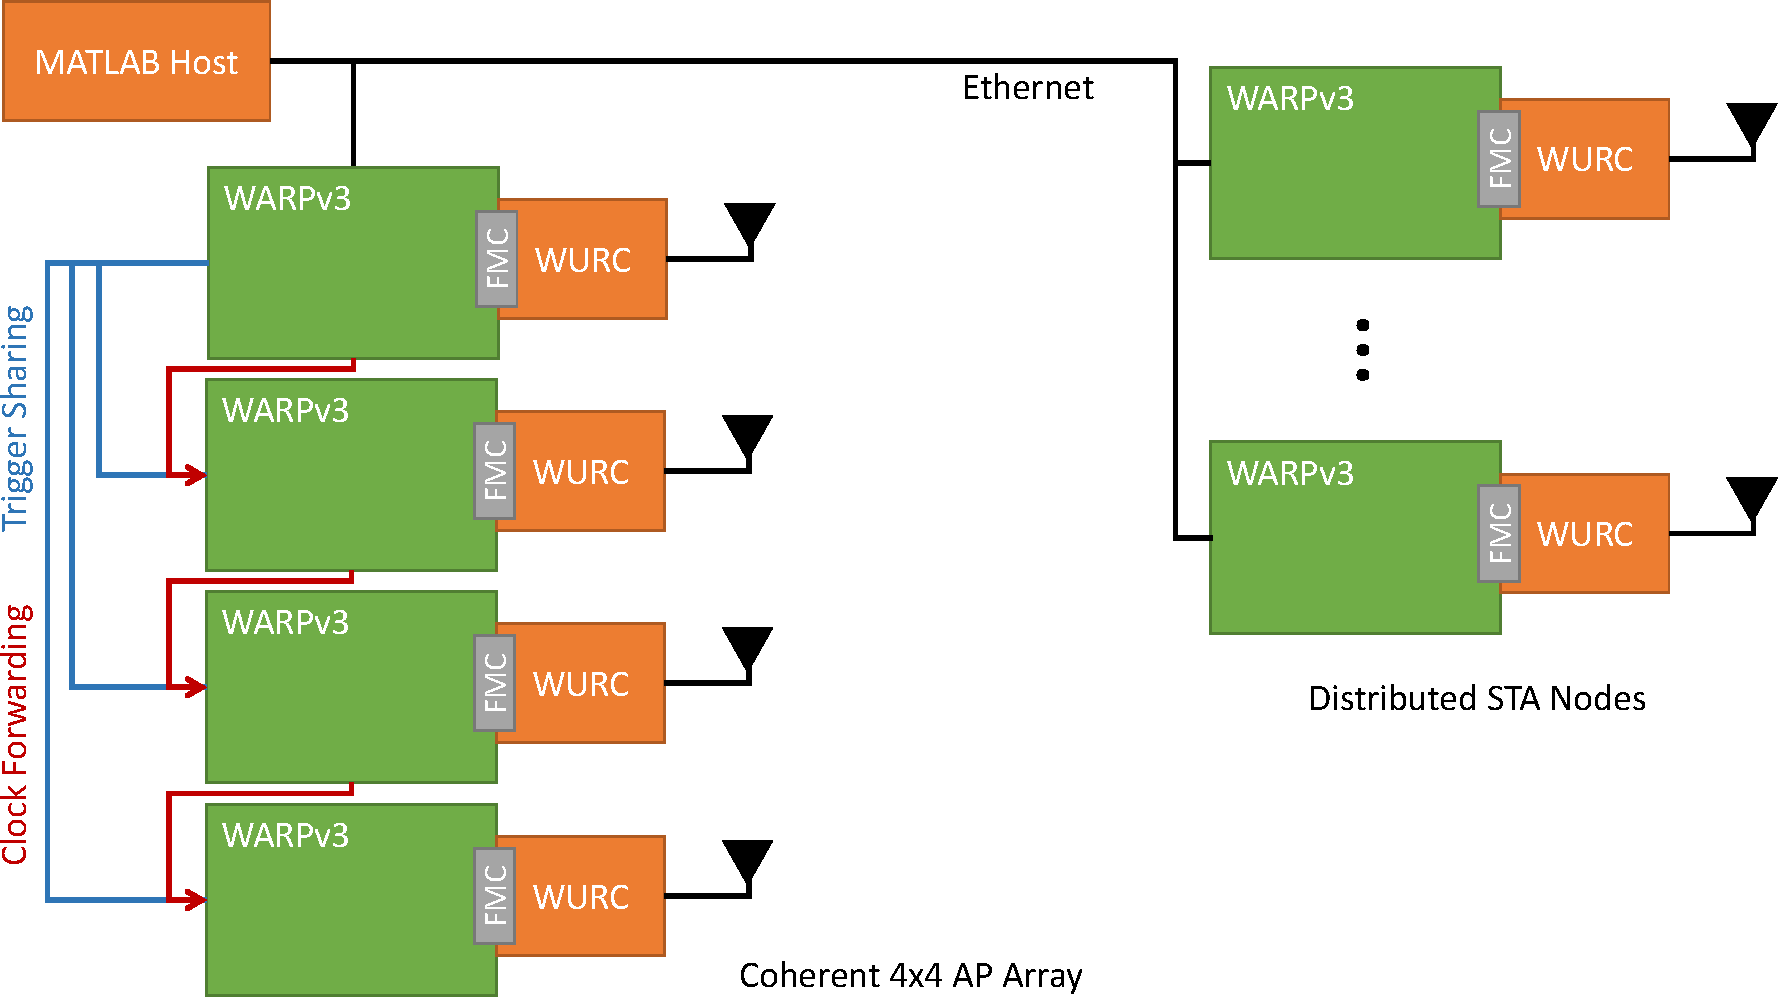
\includegraphics[width=0.9\linewidth]{./figs/wurc/wurc_warplab_sys_diagram}
\caption{System diagram of the $4\times4$ WARPLab-WURC \ac{AP} and \acp{STA}.}
\label{fig_wurc_4x4_sys_diagram}
\end{figure}

% WURC 4x4 Testbed photos
\begin{figure}[p]
\centering        
   	\subfigure[\ac{WURC} Array Internals.]{
		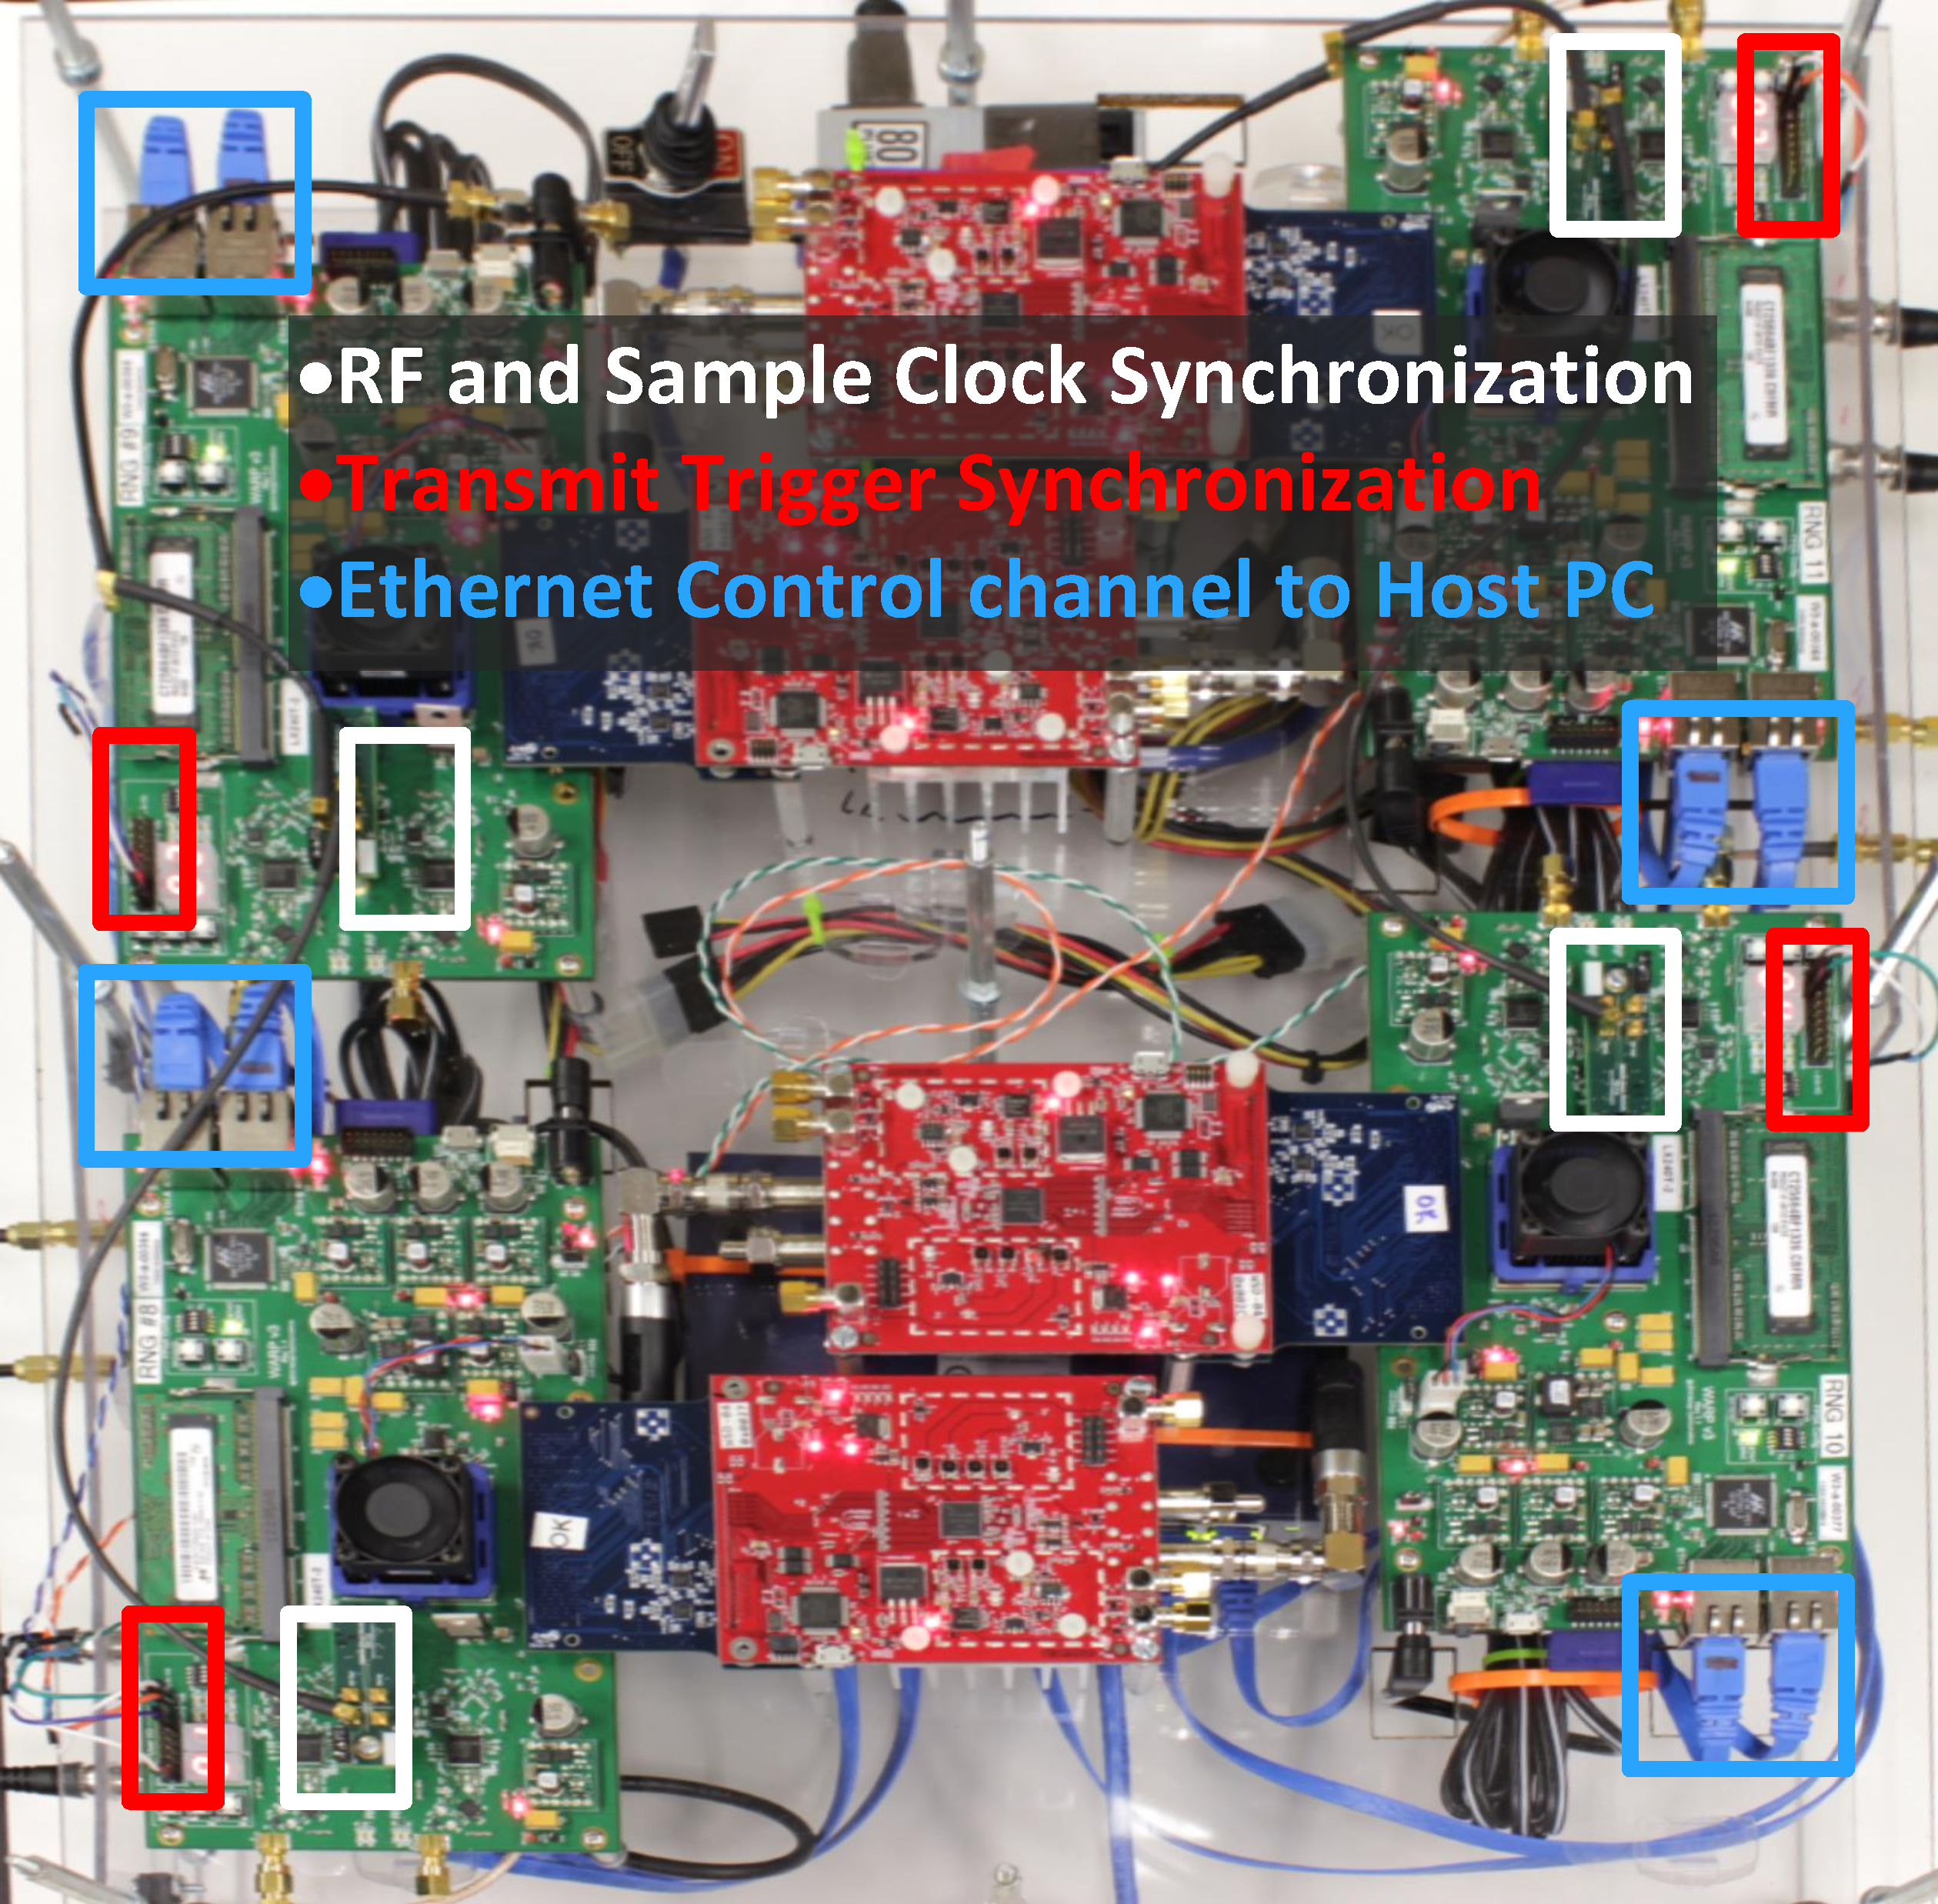
\includegraphics[width=0.45\linewidth]{figs/wurc/wurc_array_2}   \label{fig_wurcarray}
        	}
	\subfigure[\ac{WURC} Array Antennas.]{
		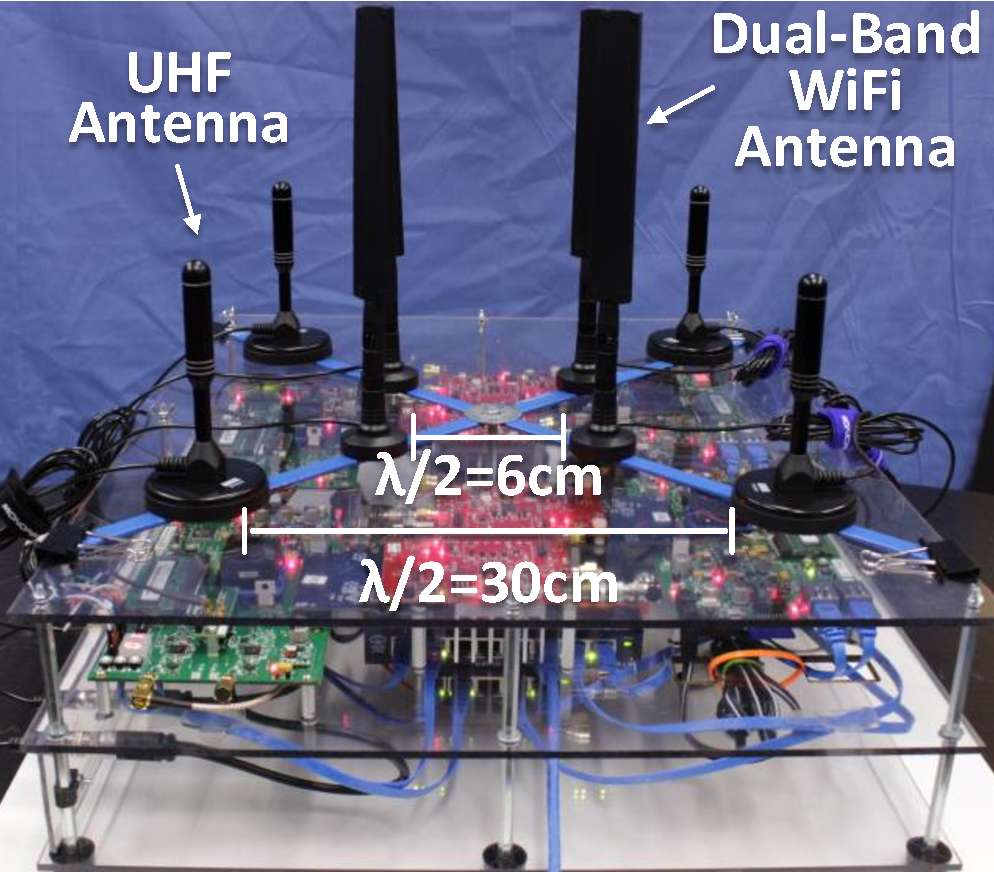
\includegraphics[width=0.45\linewidth]{figs/wurc/wurc_array_3}   \label{fig_wurcarrayTop}
        	}
\caption{Photo of the implemented $4\times4$ WARPLab-WURC \ac{AP} for UHF-band operation.
\label{fig_wurc_4x4_testbed}}
\end{figure}
	
	Utilizing the \ac{ISM}-band 2.4~GHz and 5.8~GHz radios on the WARPv3 platform as well as the 470-698~MHz UHF radios on the \ac{WURC}, we were able to build an \ac{SDR} \ac{MU-MIMO} platform with the largest operational tuning range available at the time.
	A key design consideration was to enable the use of a wide range of frequencies using the same \ac{MAC} and \ac{PHY}, allowing side-by-side comparison of performance in various RF environments.
		Each radio on each node can respectively transmit the similar 802.11af, 802.11g, and 802.11b-like \ac{OFDM} sounding and payload waveforms, controlling the \ac{PHY} implementation as an experimental variable that remains constant.
	
	The designed platform and experimental topology with an arbitrary number of distributed \ac{STA} nodes is shown in Figure~\ref{fig_wurc_4x4_sys_diagram}.


%\begin{figure}[b!]
		%\centering  
	%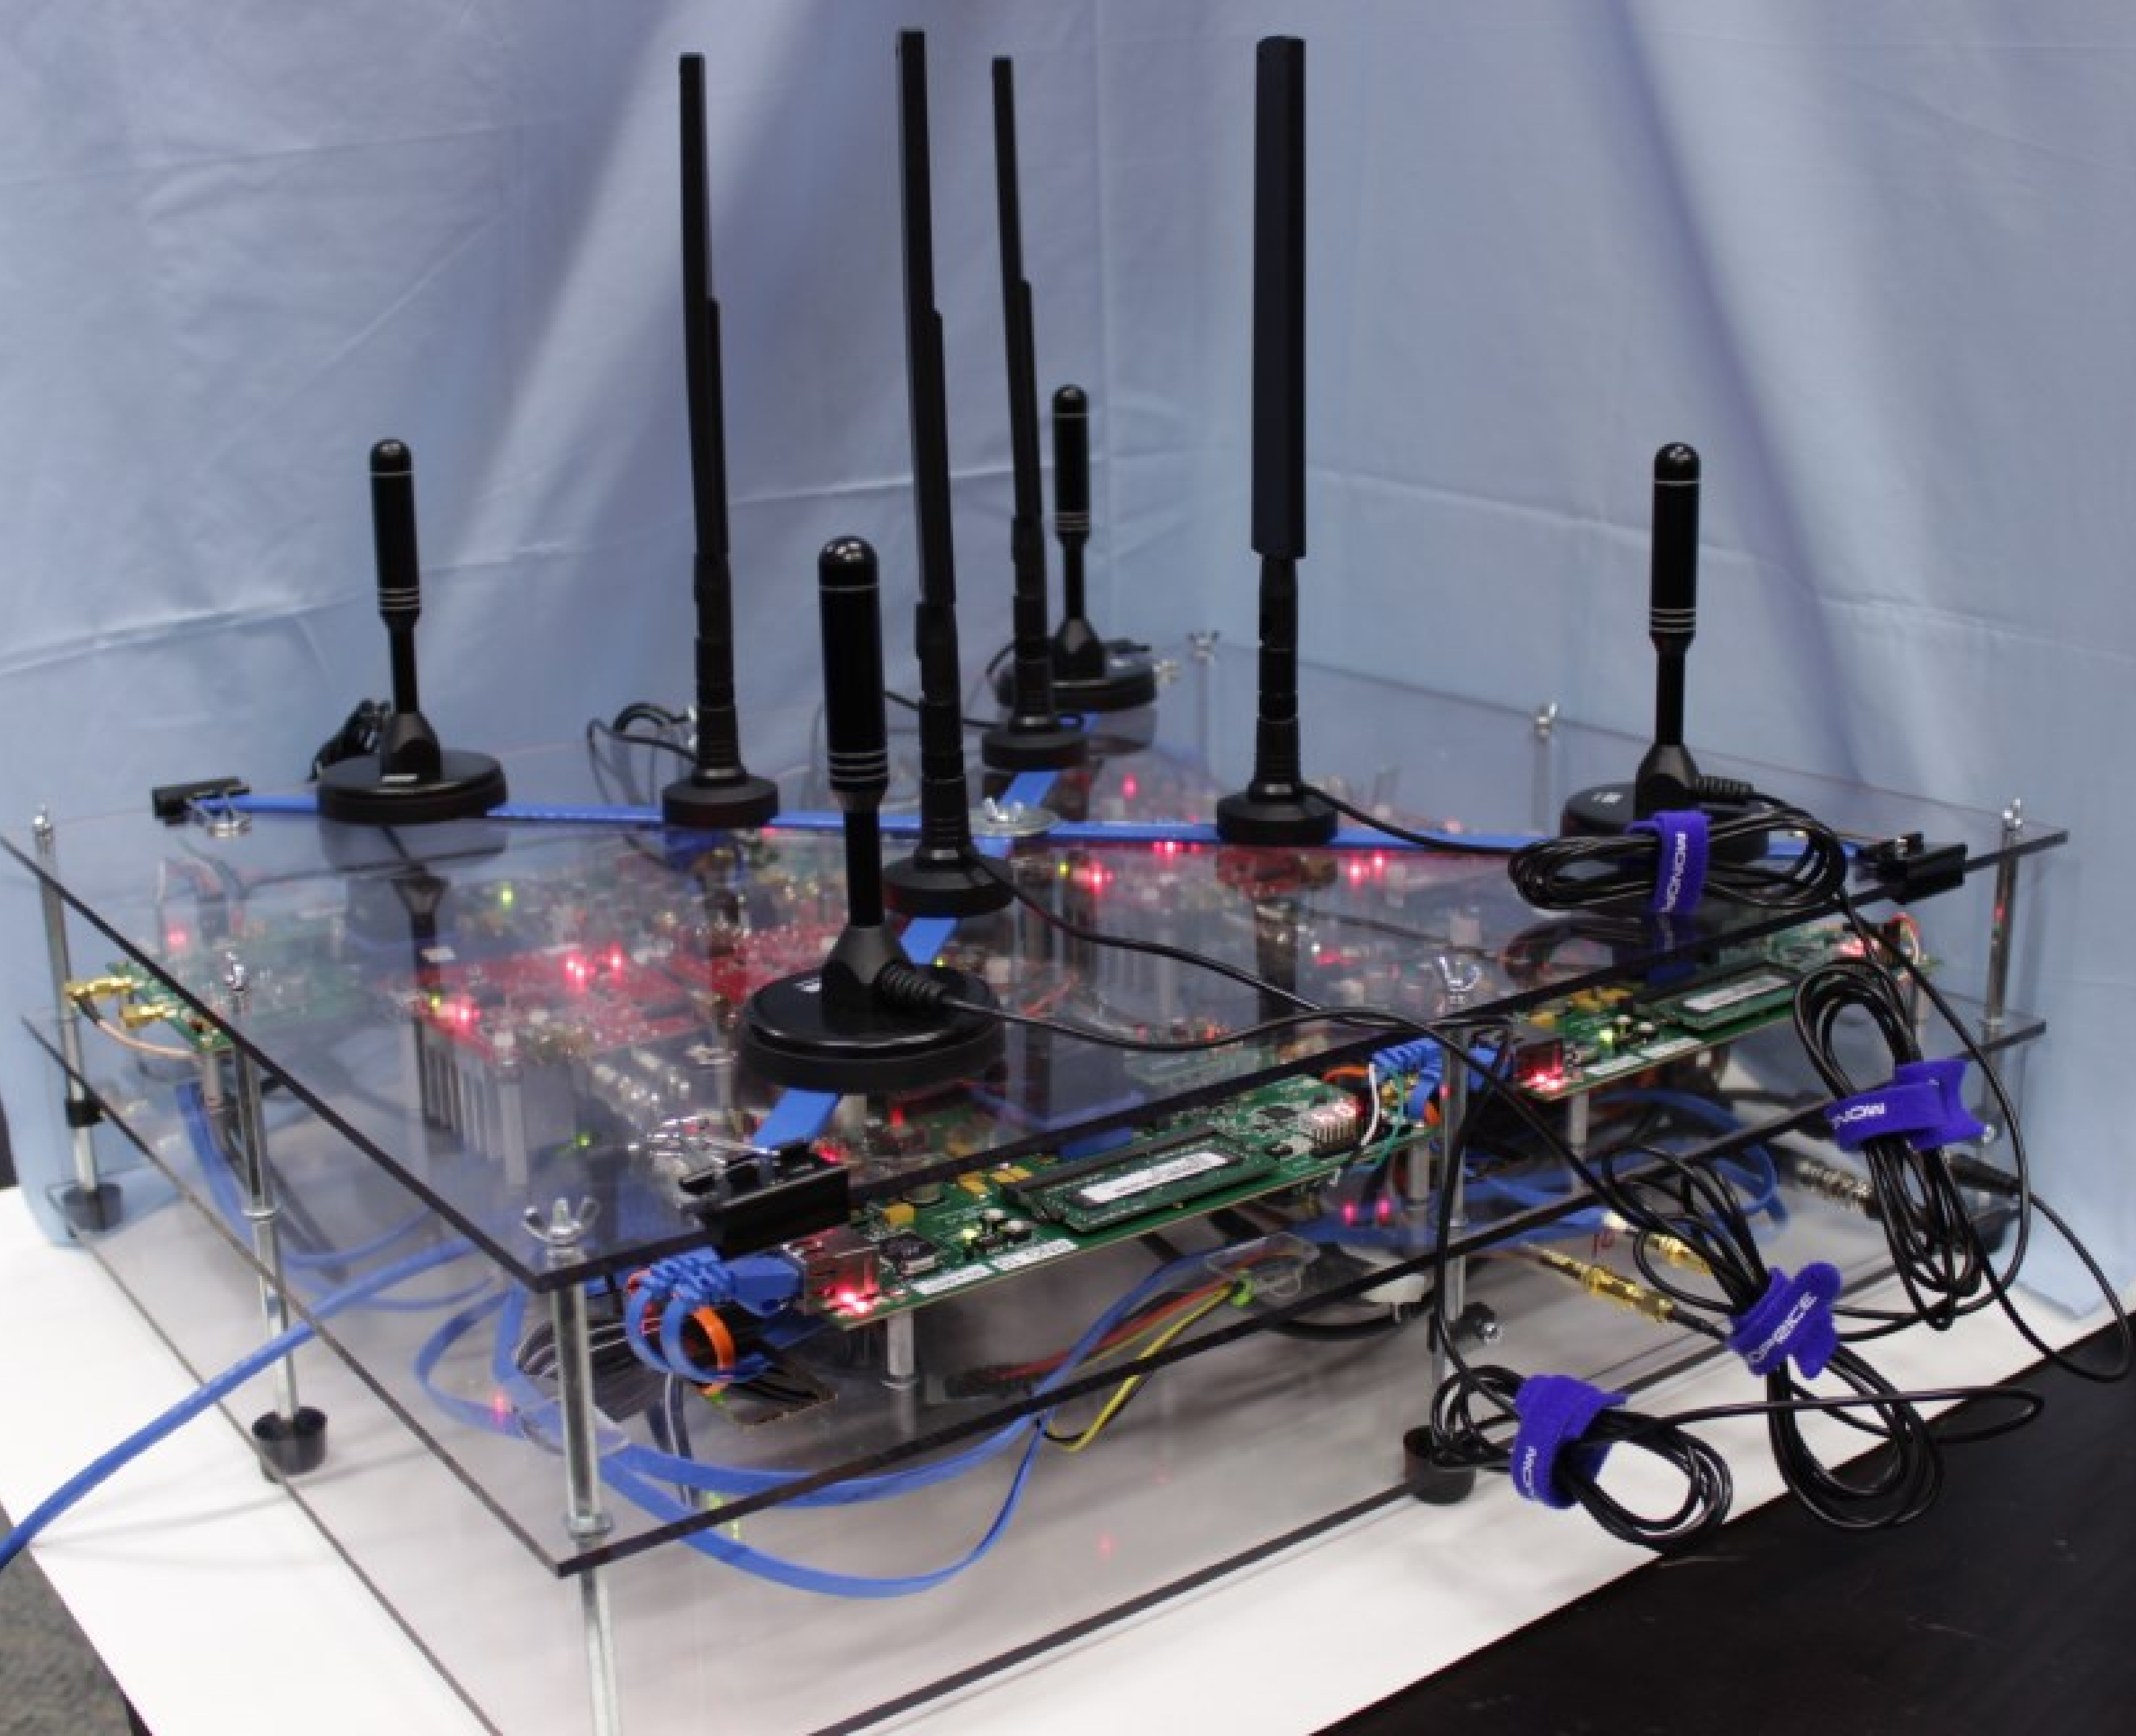
\includegraphics[width=4.5in]{figs/wurc/wurc_array_1} 
   	 %\caption{The \ac{WURC}-enabled MU-MIMO array.\label{fig:wurc_array_iso}}
%\end{figure}

%In order to evaluate \ac{MU-MIMO} transmissions at various carrier frequencies and node topologies, we integrate \ac{WURC} and four WARPv3 modules into a coherent 4-radio array.

\subsubsection{Timing and Clock Synchronization}
	The \ac{MU-MIMO} \ac{WURC} array combines four WARPv3 boards and 4 \ac{WURC} daughtercards into a single prototype base station providing combined sample and RF-reference clock synchronization, power, and structural support.
	Synchronization of reference clocks for ADC sampling and RF frequency synthesizers is required for coherent beamforming and is accomplished by forwarding a daisy-chained reference clock from one master WARPv3 baseband board to the others in the array as shown by the red clocking lines in Figure~\ref{fig_wurc_4x4_sys_diagram}
	All radios derive their sampling and RF reference clocks from this forwarded clock and thus remain phase-synchronized for transmit and receive beamforming.
	In addition, we ensure symbol timing synchronization by designating a master node that transmits a \ac{GPIO} pulse to any number of slave WARPv3 nodes in order to trigger simultaneous start of transmission as shown by the blue trigger lines in Figure~\ref{fig_wurc_4x4_sys_diagram}.

\subsubsection{Antennas}
	Most studies of UHF propagation involve large, directional antennas intended for signal reception over many kilometers.
	This is because optimal signal reception and transmission requires antennas of at least 1/2 wavelength to generate a resonating standing wave.
	On the other hand, a \ac{WLAN} deployment utilizing UHF frequencies may wish to keep the size of the base station somewhat limited, particularly for indoor deployments.
	In our experiments, we utilize off-the-shelf passive, omni-directional 3 dBi DTV antennas (August DTA240) that would provide the largest range of coverage with minimal dependance on direction.
	In our experimental platform (Figure \ref{fig_wurcarrayTop}), it is actually the dual-band 2.4/5.8 GHz band antennas (L-com HG2458-5RD-RSP with 3~dBi and 5~dBi gain, respectively) that are larger in size.

	This type of omni-directional antenna array is ideal for indoor \ac{MU-MIMO} as it provides many opportunities for multipath reflections \cite{aryafar2010design}.
	Indoor multi-path environments with reflections that are incident on the antenna from all azimuth angles are most like the \textit{i.i.d.} Rayleigh channel distributions that were first used to prove scaling benefits for many-antenna \ac{MU-MIMO} systems \cite{marzetta2010noncooperative}.
	In order to guarantee the required channel diversity, each antenna was spaced at least 1/2 wavelength for its respective transmit frequency as shown in Figure \ref{fig_wurcarrayTop}.

% ###########################
%\subsection{Software Framework}
%
%In addition to the development of custom hardware to meet our design requirements, we build upon or modify a number of existing applications in order to develop an experimental framework for the \ac{WURC} \ac{MU-MIMO} array.
%
%
%\subsubsection{WARPLab}
%\label{sec:warplab}
%
%The WARPLab 7 framework for WARP hardware provides a means to pre-compute baseband signals in MATLAB, load transmit sample buffers into an array of WARP boards, and then trigger a simultaneous RF transmission of all buffered signals via a back-end ethernet network or a GPIO trigger \cite{warp}. Similarly, an arbitrary number of radios can be configured to perform \ac{AGC} and store their received RF samples in buffers for off-line retrieval and processing.
%
%We extend WARPLab's object-oriented framework with additional classes and methods to support the \ac{WURC}'s interfaces. This system provides a powerful workflow for UHF PHY prototyping and measurement studies for multi-antenna systems. 




	\section{WURC Array 8x8}
\label{sec_wurc_8x8}

	Once we had demonstrated basic \ac{MU-MIMO} feasibility using the experimental 4x4 \ac{SDR} platform in Section~\ref{sec_wurc_4x4}, the next step was to leverage the modular design of \ac{WURC} and develop a more integrated platform suitable for scaling the beamforming performance of the system.
	
\begin{figure}[p] % WURCLab MIMO Node
\centering
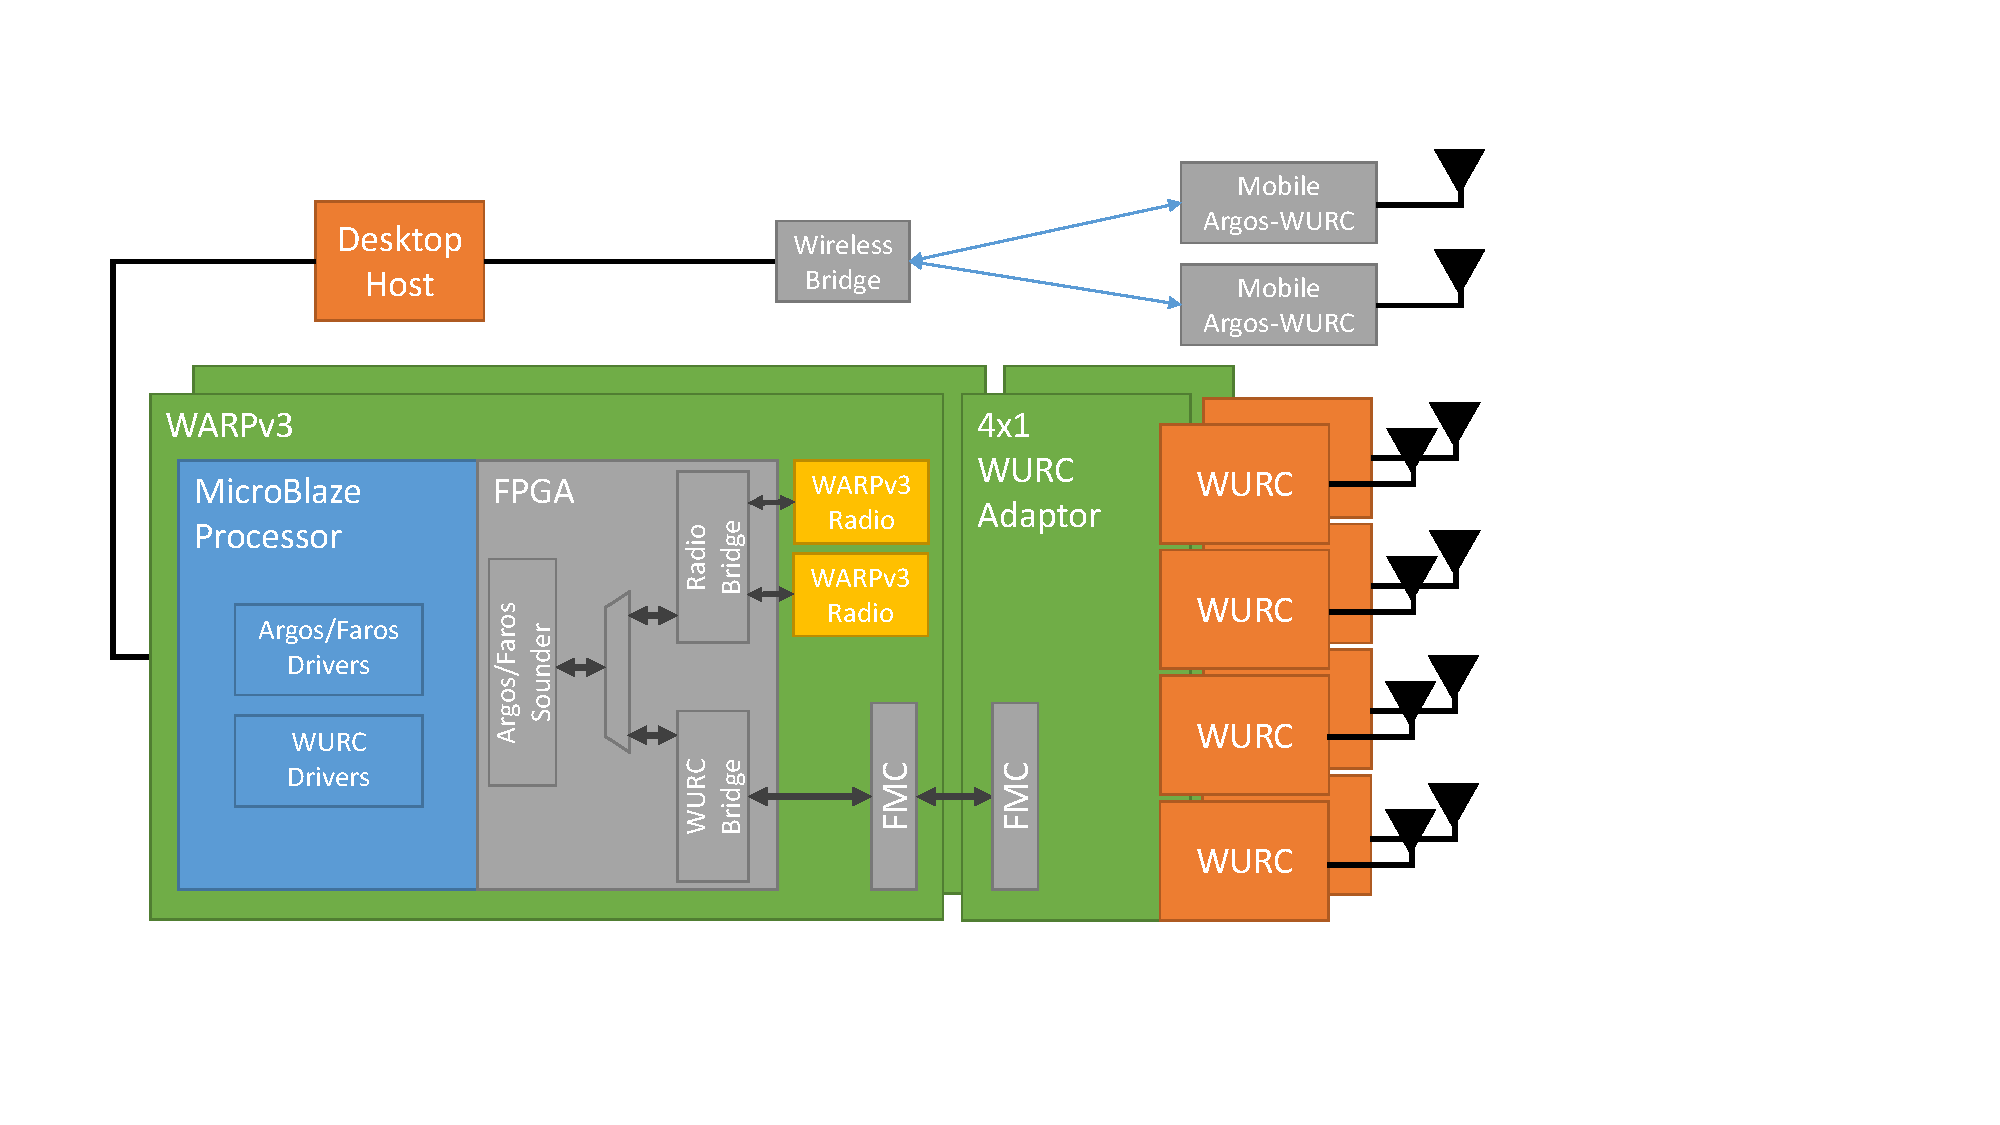
\includegraphics[width=1\linewidth]{./figs/argos-wurc_system_diagram}
\caption{System diagram of the $8\times8$ WURC \ac{AP} and mobile \acp{STA}.}
\label{fig:wurc_argos_hw}
\end{figure}


\begin{figure}[p] % WURCLab MIMO Node
\centering
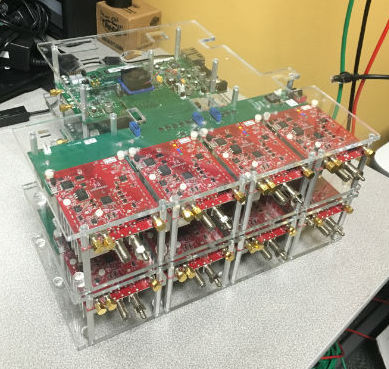
\includegraphics[width=0.7\linewidth]{./figs/MIMO_node.jpg}
\caption{Photo of the implemented $8\times8$ WURC \ac{AP} for UHF-band operation.}
\label{fig:mimohw}
\end{figure}

	Although \ac{MU-MIMO} capabilities are available on ``wave-two'' 802.11ac \ac{ASIC} chips, the research community has been limited by the lack of cross-layer observability and access that can be had on commodity hardware, making experimentation with \ac{MU-MIMO} systems difficult.
 In addition, to the best of our knowledge, no 802.11af \acp{ASIC} has yet been announced, and certainly not one that implements the maximum 4-stream with 8-transmit antennas, 8x1x1x1x1 \ac{MU-MIMO} beamforming allowed in the 802.11 standard \cite{std11af}.
 For that reason, we developed the hardware and software stack of a custom \ac{SDR} platform that allows us to arbitrarily generate, intercept, and modify \ac{MU-MIMO} transmissions that are designed to be 802.11af-compatible with 8x1x1x1x1 operation.
	In this section we discuss the architectures and challenges involved in designing and scaling our \ac{WURC}-based \ac{MU-MIMO} platform.
	
\subsection{Hardware Platform Design}
\label{sec:wurc_argos_design}

%We further extend the \ac{WURC} UHF test equipment that we developed in previous sections for rapid physical-layer prototyping in UHF bands \cite{anand2014case, WURC}.
	%\ac{WURC} was designed to enable high-power transmission up to 1~W and reception of wide-band radio signals in frequencies between 470-698~MHz \cite{WURC} and each module provides one complete analog radio chain for use with a single WARPv3 \ac{SDR} baseband \cite{warpProject}.
	%Multiple WARPv3 boards can be clock synchronized with a daisy-chained reference clock and shared sampling trigger.

	The equipment and daisy-chain topology for the 4x4 system in Figure~\ref{fig_wurc_4x4_sys_diagram} suffers from two key impairments that limit the scalability of the hardware.
	First, the system utilizes a daisy-chain clocking topology that introduces additional transmission and reception phase errors and aperture jitter as the reference clock signal is forwarded \cite{kester2008aperture}.
	The timing error introduced on each hop due to clock skew and system noise can be viewed as a zero-mean Gaussian random process where the variance of the aggregate Gaussian random process sampled at each hop increases proportionally to the number of hops.
	As the system scales from 4x4 to 8x8 and more, a daisy-chained clocking structure becomes more difficult to maintain, particularly when each interconnect is cabled and prone to damage or disconnect during transport and setup.
	
	In addition, the topology in Figure~\ref{fig_wurc_4x4_sys_diagram} also requires the sharing of a timing synchronization trigger that also suffers from signal bi-stability caused by signals crossing from one clocking domain to the next \cite{cummings2008clock}.
	When a bi-stable trigger falls on a different cycle of the destination clock in a coherent \ac{MIMO} system, it looks like a shift in channel phase equal to a full clock sampling period, and significantly disrupts coherent beamforming.
	This is a problem that can be managed in smaller-scale systems but requires more engineered solutions for large-scale systems.

	In order to address these issues and support modular, scalable, and mobile \ac{MIMO} \ac{SDR} arrays, we design, layout, and manufacture a clock-synchronized 4-radio adapter board that can connect up to 4 \ac{WURC} radio front-ends to a single WARPv3 baseband board (Fig.~\ref{fig:wurc_argos_hw}: the $4\times1$ WURC Adapter).
	With this architecture, RF reference clocks are now buffered and distributed in a tree topology, while inter-radio triggering is no longer needed since all data streams come from the same \ac{FPGA} and same clock domain.
	This has the added advantage of reducing the cost and hardware footprint of a 4-radio UHF \ac{AP} by eliminating extraneous WARPv3 boards compared to the previous design.
	
	To support the newly developed adaptor hardware, we develop the WARPLab software support (FPGA HDL, MicroBlaze C, and WARPLab extensions in MATLAB) to transparently integrate the four UHF radio front-ends with the existing WARPLab version 7.4 framework \cite{warpProject}, expanding upon the initial integration presented in Section~\ref{sec_warplab}.

\subsubsection{Antennas.}
\label{sec_8x8_antennas}

	Our over-the-air experiments utilize omni-directional 3~dBi August DTA240 portable UHF antennas for the \ac{AP}, mobile \acp{STA}, and indoor \acp{STA} while the static outdoor \acp{STA} use Comtelco Y42400WB 7~dBi log-periodic antennas.
	During experiments, the \ac{AP} antennas are configured in a linear array separated by a minimum of $\lambda/2$ distance to ensure sufficient de-correlation of the received signals.


%\subsubsection{Wireless Mobility.}
%\label{sec_8x8_backhaul}
%
	%Another key upgrade to the experimental design o
	%
	%\cite{shepard2015faros}


	\section{Scalable RF Clock Synchronization}
\label{sec_iris_clocking}

	Stable, low-noise, and synchronized clocking is necessary for a coherent \ac{MIMO} array.
	For example, when a noisy reference clock is used for \ac{ADC} or \ac{DAC} sampling clocks it results in \textit{aperature uncertainty} error \cite{brannon2006jitter} by causing the system to sample at non-ideal and randomly-varying time intervals.
	When the noisy reference clock is used as a reference for carrier synthesis, it manifests as \textit{phase noise} in the input and output RF signal \cite{an687}.
	
	In addition to the noise caused by RF reference clock jitter, additional transceiver impairments such as carrier frequency offset of the radio's frequency mixer circuits and sample frequency offset of the radio's \acp{ADC} rapidly degrades the performance of \ac{ZFBF} in even small $4\times 4$ systems \cite{rogalin2014scalable}.
		Theoretical studies of many-antenna systems in the presence of phase noise have shown that this noise source can result in well over 50\% or more decrease in sum throughput in both the many-antenna uplink \cite{krishnan2014impact} and downlink \cite{pitarokoilis2012effect} systems.
	As \ac{MIMO} systems increase in size, the generation and distribution of a reference clock becomes a more difficult system-level design challenge whether for a single co-located array of radios or in a distributed \ac{MIMO} system such as those proposed for 5G cellular \cite{cui2014evolution, ali2014evolution}.
	
	In this section, we present the design and evaluation of a number of different practical clocking topologies in large-scale coherent \ac{SDR} systems, presenting new measurement results of unique clocking topologies that we have implemented.
	Based on our insight gained from developing the $8\times 8$ \ac{WURC} \ac{SDR} in Section~\ref{sec_wurc_8x8} we present a novel daisy-chained clocking architecture for next-generation systems that increases the number of radios while reducing the amount of cabling required compared to other large-scale \ac{MU-MIMO} systems.
	Consequently, reliability and portability is improved.
	
	Another consideration for large-scale \ac{TVWS} systems is that the large size of antennas spaced at a half-wavelength for spatial diversity will need to be addressed.
	We develop a robust, distributed, and low-cost system for distributing an RF reference clock with a daisy-chain radio topology as a new approach to solving this challenge.
	An added benefit is that the modularity of the design yields freedom when considering the physical configuration of the radios and can enable new experiments in distributed \ac{MIMO}, \ac{CoMP}, and other coherent radio technologies at very large scale.

%\rgnote{This section is the new work I've done on the Iris platform that Dr. Zhong asked for and is beign finalized right now. A discussion regarding clock synchronization techniques, GPS timing synchronization and how it is not appropriate for coherent CoMP (seriously, literally everyone I talk to about CoMP brings this up incorrectly), and a measurement study of our innovative clock regeneration scheme for Iris that ensures essentially unlimited clock domain scaling and absolute deployment flexibility vs. all other approaches I've seen to date. This section builds on the concept in sections, presenting the clocking structure design and evaluation for WURC, WURC Array, IRIS, then finally Faros as the evolution of scalable clocking.}



%###############################################
\subsection{Cooperative Multi-Point and Network \ac{MIMO}}
\label{sec_comp_brief}

% Table generated by Excel2LaTeX from sheet 'Sheet1'
\begin{table}[h]
  \centering
  \caption{Comparison of CoMP Techniques and Required System Support.}
  \resizebox{1\textwidth}{!}{%
    \begin{tabular}{llllll}
          & \multicolumn{5}{c}{\textbf{Coordinated Multi-Point (CoMP)}} \\
\cmidrule{2-6}          & \multicolumn{2}{c}{\textbf{Coordinated Switching/Beamforming (CS/BF)}} & \multicolumn{3}{c}{\textbf{Joint Processing (JP)}} \\
\cmidrule{2-6}          & \multicolumn{1}{c}{\multirow{2}[2]{*}{\textbf{Coordinated Beam-Switching (CBS)}}} & \multicolumn{1}{c}{\multirow{2}[2]{*}{\textbf{Coordinated Switching (CS)}}} & \multicolumn{2}{p{12.64em}}{\textbf{Joint Transmission (JT)}} & \multicolumn{1}{c}{\multirow{2}[2]{*}{\textbf{Dynamic Point Selection (DPS)}}} \\
          &       &       & \multicolumn{1}{c}{\textbf{Coherent}} & \multicolumn{1}{c}{\textbf{Non-Coherent}} &  \\
    \midrule
    \midrule
    \textbf{User Data Location} & One BTS & One BTS & All   & All   & All \\
    \textbf{Pre-coding Decision} & Individual & Individual & Joint & Individual & Individual \\
    \textbf{Timing Sync Needed} & \cellcolor[rgb]{ .922,  .945,  .871}Yes & \cellcolor[rgb]{ .922,  .945,  .871}Yes & \cellcolor[rgb]{ .922,  .945,  .871}Yes & \cellcolor[rgb]{ .922,  .945,  .871}Yes & \cellcolor[rgb]{ .922,  .945,  .871}Yes \\
    \textbf{Clock Sync Needed} & \cellcolor[rgb]{ .949,  .863,  .859}No & \cellcolor[rgb]{ .949,  .863,  .859}No & \cellcolor[rgb]{ .922,  .945,  .871}Yes & \cellcolor[rgb]{ .949,  .863,  .859}No & \cellcolor[rgb]{ .949,  .863,  .859}No \\
    \end{tabular}%
	}
  \label{tab_comp_types}%
\end{table}%


	\ac{CoMP} typically refers to multi-cell transmit coordination \cite{ali2014evolution} for improving user signal strength or mitigating inter-cell interference.
	However, taken to its limit, a logically modular, coherent, and distributed \ac{MIMO} system may not have a clear concept of a ``cell.''
	For example: clusters of coherent \ac{WURC} radios could be distributed across a rooftop or across an office ceiling to provide ubiquitous coverage and large array aperature size.
	For the purpose of this discussion, we will define \ac{CoMP} as the simultaneous use of transmitters that are physically located much further than a single wavelength apart in order to increase signal strength and reduce interference in a wireless network.
		
	There are many different types of inter-cell or inter-\ac{AP} coordination, each with their sets of system requirements and tradeoffs.
	We present an overview of \ac{CoMP} techniques in Table~\ref{tab_comp_types} corresponding to the taxonomy proposed by Ali et. al. \cite{ali2014evolution} in order to clarify our target system design; for more details regarding these techniques, we direct the reader to the references therein.
	Other work has shown that while the system burden can be quite high, the performance of coherent \ac{JT}-\ac{CoMP} consistently outperforms other techniques for users at the cell edge \cite{cui2014evolution, kim2017call}, and is one of the few techniques that increases network spectral efficiency, making it very desirable for next-generation networks.
	
	We focus on delivering a scalable, physical layer clock synchronization solution that enables coherent \ac{JT}-\ac{CoMP} or, equivalently, ``network \ac{MIMO}'' \cite{huh2012network}.
	
		At this point, it is useful to define a few terms that will be useful for this discussion.
	Relative clock \textbf{skew} is the time difference between two clocks as defined by their edge, or the relative point in time when two clock signals cross a voltage threshold.
	Clock \textbf{jitter} is the short-term variation in clock frequency, often empirically measured as the \ac{TIE}, or the distribution of error between the actual clock edge and an ideal clock edge over a large sample size.
	Clock \textbf{wander} is the long-term variation in clock frequency, sometimes characterized as frequency dynamics occuring below 10~Hz.
	Finally, we will use the term \textbf{syntonized} to refer to two clocks that have the same oscillation frequency, but may each have arbitrary phase relative to each other; once those two clocks share absolute phase (or have information regarding the offset such that it can be removed or ignored), then they are considered \textbf{synchronized}.
	
%###############################################
\subsection{Alternative Distributed Clocking Architectures}
\label{sec_comp_alts}

\textbf{Massive MIMO Clocking.}
	Several Massive \ac{MIMO} testbeds have been constructed from \ac{NI} hardware using the \ac{NI} CDA-2990 or ``OctoClock'' to form a two-tiered or radial clocking network with coaxial cables linking back to a grand master reference clock \cite{luther20145g}.
	Identical hardware and clocking topologies have been reported for the testbeds used by Lund and Bristol Universities \cite{vieira2014flexible}, as well as Facebook Project ARIES \cite{choubey2016introducing}.
	Previous generations of many-antenna systems at Rice University have also used a similar, flat clocking topology \cite{shepard2012argos, shepard2013argosv2}.
	Both timing and synchronization are accomplished via flat or tiered clock distribution buffers and each link requires a coaxial cable for both clock distribution and timing synchronization reference, resulting in large, bulky systems.
	
\textbf{GPS-Disciplined Oscillators.}
	Jungnickel et. al. report a carrier frequency offset of $6\cdot10^{-10}$ between two Rubidium GPS-conditioned oscillator platforms after 24 hours of outdoor signal conditioning \cite{jungnickel2008synchronization}.\footnote{It might be unintuitive at first glace, but \ac{GPSDO} platforms increase in precision over time as they integrate more timing observations from more \ac{GPS} satellites.}
	This corresponds to 0.6~ppb at their 10~MHz reference, or 3.12~ppb at 52~MHz, the reference frequency of our system's \ac{MEMS} oscillators with 100~ppb accuracy.
	The authors claim that syntonization between \ac{JT}-\ac{CoMP} points is not required since residual carrier offset can be tolerated.
	Nevertheless, their system only demonstrates a low-order $2\times 2$~\ac{ZFBF} and required a \ac{GPS} synchronization period of 24 hours before the \ac{GPS} oscillators had sufficient observations to avoid excessive noise with 5~ms of time between channel sounding and \ac{ZFBF} transmission.
	This represents a relatively easy demonstration case since longer transmission intervals with older \ac{CSI} would have required even lower carrier frequency offset than that demonstrated, and our system targets array sizes much larger than two radios which increases the performance requirements proportionally.
	With the inability to practically operate indoors or at large time scales between refreshing \ac{CSI}, we disagree with the author's conclusion that RF syntonization is not necessary for large-scale \ac{CoMP}.
	
\textbf{Over-the-Air Synchronization}
 Rogalin et. al. proposed an over-the-air frequency synchronization and offset compensation algorithm that allowed distributed \ac{MIMO} nodes to perform coherent operations \emph{without} syntonization; however the achievable rate degrades extremely rapidly due to clock drift over the course of \emph{milliseconds} in just a $4\times 4$ system (28\% loss of achievable rate over 16~ms, \cite{rogalin2014scalable}, Figure 5).

	For these reasons, we argue that syntonization is a system-level requirement for \ac{JT}-\ac{CoMP} with many radios and that \ac{GPS} and over-the-air techniques proposed in the literature are inadequate for large-scale distributed systems.
	
\textbf{White Rabbit.}
	The White Rabbit Project seeks to solve a similar distributed clock and timing synchronization problem.
	Custom networking hardware was developed for the \ac{CERN} Large Hadron Collider experiment and manufactured by Seven Solutions S.L., \cite{lipinski2011white, serrano2013white} utilizing a Layer 1 Synchronous Ethernet (Sync-E) switching network \cite{rec2007g} for syntonization, the IEEE1588 \ac{PTP} protocol for coarse synchronization, and a custom \ac{DDMTD} algorithm to fine-tune clock phase offsets in order to produce distributed clock synchronization with sub-ns accuracy \cite{wlostowski2011precise}.

In our solution, we seek to remove the hardware complexity, cost, and deployment restrictions of large-scale radial or tiered clock distribution topologies while achieving the high-precision syntonization among a distributed set of coherent radios achievable with White Rabbit.
	Our key observation is that unlike the White Rabbit solution, coherent \ac{CoMP} requires only syntonization, provided all timing events are deterministic without variable delay exceeding some threshold.
	For instance, there are significant provisions within White Rabbit to compensate for the light propagation delay for uplink vs. downlink fiber lasers that are not necessary in a system-level design of a \ac{JT}-\ac{CoMP} radio access network.
	
	This relaxation of our \ac{CoMP} system requirements compared to those of the Large Hadron Collider results in the ability to design a distributed, high-precision clocking architecture that utilizes a commodity Layer 1 synchronous fiber-channel Ethernet backplane.
	This design can be implemented with little additional hardware components on the distributed radio heads compared to White Rabbit hardware implementations.
	A benefit of this system design choice, shared with White Rabbit, is that \ac{JT}-\ac{CoMP} requires user data to be distributed to the cooperating base stations anyway, so re-using the existing data backplane for high-precision clock distribution is ideal.

\pagebreak

%###############################################
\subsection{Tiered Modular Clock Synchronization}
\label{sec_tiered_clocking}

%\rgnote{Tiered clocking: what I did for WURC and 4x1 WURC with a flat clocking hierarchy}

Since the transmit and receive chains in a \ac{MU-MIMO} base station require precise phase synchronization, \ac{WURC} was designed to draw RF reference clocks from the host digital baseband board as shown in Fig.~\ref{fig:wurc_clock_diagram}.
This simplifies the digital design since both the \acp{DAC} and \acp{ADC} are driven with the same clock as the rest of the digital signal processing path in the \ac{FPGA}.

%\rgnote{Discussion of FPGA and native clocking jitter and the evolution of the adaptor design based on iterative measurements and testing.} 

\begin{figure}[h]
\centering
  \includegraphics[width=4.5in]{figs/clk/wurc_clock_diagram_2}   
    \caption{Source-synchronous sampling clocks and RF reference clocks are buffered in stages, permitting fanout to up to 4 radios.}
\label{fig:wurc_clock_diagram}
\end{figure}

We placed an additional RF reference and sampling clock buffer, a Texas Instruments LMK001055, on the FMC/HSMC adapter rather than on the daughtercard itself so that the designed system can scale up to four \ac{WURC}s driven from a single host FPGA with synchronized clocks.
A single forwarded clock branch is used in the 1:1 HSMC/FMC adaptor shown in Figure~\ref{fig_warp_wurc_hw}, however the full 4 branches of clock buffering available in the design was used in the 4:1 HSMC/FMC adaptor used in the $4\times 4$ and $8\times 8$ \ac{WURC} arrays shown in Figures~\ref{fig:wurc_argos_hw} and \ref{fig:mimohw}.

Multi-tiered clocking trees have been proven out in the literature, in industry, and in our first \ac{WURC} \ac{SDR} platform as a reliable and manageable way to create coherent multi
Nevertheless, when we consider the task of delivering a single reference clock to potentially hundreds of discrete radios, the tiered topology quickly becomes unwieldy.
In the following section, we evaluate a new clocking architecture that addresses these concerns using next-generation \ac{SDR} hardware. 



%###############################################
\subsection{Multi-Hop Clock Synchronization}
\label{sec_daisy_chain_clocking}
	
In this section, we present the design and evaluation of a key architectural innovation required to scale our $8\times 8$ \ac{WURC}-array by an order of magnitude to 100s of radios that we designed and implemented on a new generation of commercial \ac{SDR} hardware.
	This newer ``IRIS-020'' and ``IRIS-030'' \ac{SDR} radio hardware is informed by our experience implementing the \ac{WURC} radio arrays, but for the sake of brevity, we will omit most of the system design since it architecturally mirrors that of \ac{WURC}.
	Instead, we will focus in this section on the design of IRIS's new many-radio clocking architectures as the primary research contribution of this new platform.

	An important feature of the IRIS \ac{SDR} hardware design is the ability to provide reference clock synchronization to a very large chain of Iris modules in order to act as a single, coherent array.
	In such an array, ensuring the integrity and accuracy of the RF reference clock is extremely important, since reference clock jitter manifests as noise in the digitized signal, potentially limiting system performance \cite{brannon2006jitter}.
	
	The design goal for the IRIS-020 system shown in Figure~\ref{fig_iris_pictures} (left) was to achieve a forwarded clock phase jitter less than 3~ps RMS given the initial system design parameters of 40~MHz modulation bandwidth and \ac{ADC} resolution of 10 bits \cite{brannon2006jitter}.
	This prototype \ac{SDR} module utilized a daisy-chained clock fanout buffer topology that buffered the reference clock signal at each intermediate node before forwarding to the next node (Figure~\ref{fig_020_chain})
	
% Daisy Chain Clocking Diagram- 020
\begin{figure}[p]
\centering
\includegraphics[width=0.7\textwidth]{figs/clk/iris020_diagram}
\caption{Block diagram of IRIS-020 buffered daisy chain clocks.}
\label{fig_020_chain}
\end{figure}

% Daisy Chain Clocking Diagram -030
\begin{figure}[p]
\centering
\includegraphics[width=0.9\textwidth]{figs/clk/iris030_diagram}
\caption{Block diagram of IRIS-030 jitter cleaned daisy chain clocks.}
\label{fig_030_chain}
\end{figure}
	
	The improved design goal for the IRIS-030 system shown in Figure~\ref{fig_iris_pictures} (right) was to achieve a forwarded clock phase jitter less than 1.5~ps RMS given system design parameters of 80~MHz modulation bandwidth and \ac{ADC} resolution of 10 bits \cite{brannon2006jitter}.
	This \ac{SDR} module utilizes a daisy-chained clock jitter cleaner at each intermediate node in order to filter clock phase noise at each step and re-synthesize RF and baseband reference clocks from the cleaned clock and forward to the next node (Figure~\ref{fig_030_chain}).
	
	Based on these specifications, we chose to use a temperature-controlled MEMS oscillator for the IRIS-020 with a specification of 1.7~ps \ac{RMS} period jitter and a clock buffer IC with a specification of 0.02~ps additive phase jitter to minimize additive jitter from forwarded steps.
	The IRIS-030 received an improved specification of 0.8 \ac{RMS} period jitter to match the more stringent specifications for the later design.
	
	The clock jitter cleaner topology and general clocking diagram for the IRIS-030 is presented in Figure~\ref{fig_030_clk_diagram}.
Upstream clocks are filtered through a high-performance \ac{PLL} and digitally-controlled frequency synthesizer, Si5344, which generates low-jitter reference clocks for the high-speed serializer circuits, \ac{DAC}/\ac{ADC} blocks, and RF frequency synthesizers.

We tested the clocking jitter using the jitter measurement feature of a Keysight DSO8040B 40 GSa/s oscilloscope and three operational IRIS-020 prototypes with daisy-chained clocks, comparing their results to that of a set of four daisy-chained IRIS-030 modules with jitter-cleaned clocks.
Figure~\ref{fig_iris_pictures} shows the implemented radio clock chain hardware, representing a 6-radio \ac{MIMO} cluster (left) and an 8-radio \ac{MIMO} cluster (right).

% Iris Clocking Diagram with Jitter Cleaning
\begin{figure}[p]
\centering
\includegraphics[width=1\textwidth]{figs/clk/iris_clocking_diagram}
\caption{Diagram of IRIS-030 clocking system with jitter cleaner.}
\label{fig_030_clk_diagram}
\end{figure}



% Daisy Chain Clocking Setup
\begin{figure}[p]
\centering
\includegraphics[width=1\textwidth]{figs/clk/iris020_iris030_pics}
\caption{Test setup for IRIS-020 (left) and IRIS-030 (right) clocking measurements.}
\label{fig_iris_pictures}
\end{figure}

% Buffered vs. Cleaned Jitter Performance
\begin{figure}[p]
\centering
\includegraphics[width=1\textwidth]{figs/clk/iris_jitter_barplot}
\caption{Measured clock RMS TIE jitter as a function of the number of daisy-chain hops for both IRIS-020 (buffered) and IRIS-030 (jitter cleaned) daisy-chains.}
\label{fig_multihop_jitter}
\end{figure}

	At the time of the measurement, only three prototype IRIS-020 units were available for characterization.
	Furthermore, the equipment available at the time could not directly measure phase jitter noise spectra; instead we chose to measure RMS Time Interval Error (TIE), which is loosely equivalent, yet on a different measurement scale \cite{an687}.
	Forwarded output clock jitter measurements were made from over 10,000 recorded clock transitions at each output stage of the clocking daisy chain.
	We compared the buffered clock forwarding on the IRIS-020 module with that of the jitter-cleaned clock forwarding on the IRIS-030.
	The recorded measurements in Figure~\ref{fig_multihop_jitter} are given in picoseconds of RMS time-interval jitter. The targeted 1.5~ps RMS TIE jitter target is given as the black solid line.
	The DSO80404B has a 0.85 ps rms TIE jitter measurement floor shown as the red dotted line.
	
	For the buffered clock forwarding scheme, we observed a maximum of 0.07 ps additive TIE jitter for each additional daisy chained IRIS-020 module, which is consistent with our target specifications, but which provides little margin for additional chain length.
	In addition, we found that the orientation and order of modules impacted our measurements significantly, since the output buffer jitter proved to be very sensitive to the cable connections for input and output clocking within the daisy-chain.
	In the middle of the chain, any weak connection or poor cable would decrease the quality of the clock for the rest of the downstream chain significantly.
	The results presented in Figure~\ref{fig_multihop_jitter} are the best-case measurements out of the set of data observed in order to best represent the buffered clock topology rather than any particular physical implementation of it.
	
	This issue of noisy channels for forwarded clocks on the IRIS-020 was addressed in the later IRIS-030 design by the use of direct-attach connectors without cabling as well as the use of differential clock signaling, which proves to be more robust to common-mode noise.
	In addition, the clock jitter cleaner topology shown in Figure~\ref{fig_030_clk_diagram} provides the ability to filter jitter from the clocking signal at each step as it moves down the daisy-chain.


% Iris Jitter Cleaned Clock
\begin{figure}[p]
\centering
\includegraphics[width=1\textwidth]{figs/clk/iris030_multihop_jitter}
\caption{IRIS-030 reference clock jitter as a function of daisy chain hops.}
\label{fig_030_clk_jitter}
\end{figure}


In Figure~\ref{fig_030_clk_jitter} we show the measured \ac{RMS} \ac{TIE} jitter \ac{PDF} for each hop of the IRIS-030 chain shown in Figure~\ref{fig_iris_pictures} (right).
We find that the noise \ac{PDF} does appear to be Gaussian, with a mean relative to the measurement time base that is arbitrary, indicating that the forwarded clocks are, in fact, syntonized, with similar jitter distributions at the output of the clock jitter cleaners. 

This experimental setup was repeated with a longer chain of 10x IRIS-030 modules shown in Figure~\ref{fig_10x_hop_setup} with similar findings: for up to 10x daisy-chain hops, the successive clock jitter cleaning stages keep reference clock jitter well below the threshold for measurement with the test equipment used.
The use of 1.8~V \ac{LVDS} for clock forwarding provided additional systemic noise immunity.

% Jitter comparisons of various hardware and IOs.
\begin{figure}[h]
\centering
  \includegraphics[width=1\linewidth]{figs/clk/030_clocking_chain}   
    \caption{Test setup with 10x daisy-chained IRIS-030 modules with Si5344 development board on the second hop.}
\label{fig_10x_hop_setup}
\end{figure}


% Jitter comparisons of various hardware and IOs.
\begin{figure}[h]
\centering
  \includegraphics[width=1\linewidth]{figs/clk/iris_jitter_common_things}   
    \caption{Experimental comparison of \ac{RMS} \ac{TIE} jitter for various clock sources and \ac{FPGA} I/O standards.}
\label{fig_jitter_comparisons}
\end{figure}

Although provided in vendor specification sheets, we took the extra step of comparing the reference clock jitter of clocking outputs of the various generations of equipment used in our test setups and show the resulting \ac{RMS} \ac{TIE} jitter measurements in Figure~\ref{fig_jitter_comparisons}.

Based on our measurements, the noise on the output of the jitter cleaner on the IRIS-030 has the lowest \ac{TIE} value, with the source SiT5256 (``IRIS Oscillator'') reference a close second.
The buffered reference clock sourced from an SiT5000 oscillator on the IRIS-020 module has slightly better performance than the original WARPv3 reference hardware, which we can attribute to the method of directly probing the oscillator pads on the WARPv3 hardware with a single-ended probe while we used a coaxial cable to measure the IRIS-020 reference clock.
This reference derived from the SiT5000 has just about the same performance as a modern-day \ac{LVDS} output from an UltraScale Zynq, whereas the WARPv3 Vertix-6 CMOS I/O architecture has extremely high clocking noise.

In conclusion, we empirically demonstrate that the coherent clock distribution system behaves as designed in-situ across various platforms, and provide a direct comparison allowing the future system designer to trade cost (jitter cleaner hardware is expensive in both energy and price) against RF performance (maximum modulation bandwidth supported by system clock jitter) in future designs.


%###############################################
\subsection{Distributed Multi-Hop Clock Synchronization}
\label{sec_clk_sfp}

In this final section, we put the pieces together to implement and test a distributed, coherent \ac{MIMO} RF clock distribution network using the recovered clocks from fiber channel links in order to provide syntonicity to physically separate radio clusters.
In this design, we use a 64B/66B encoder/decoder pair to embed and recover the serial clock reference implicitly included in a high-speed serial link \cite{toyoda2010100gbe}.
The 64B/66B encoder ensures that level transitions are always present in the serial data stream, thus enabling Xilinx \ac{PHY} transceiver primitives to recover and export the reference clock, which remains syntonized to the input serial stream.
On Synchronous Ethernet systems such as the Arista 7150S SFP+ switch hardware used in our evaluation, the source serial transmitters share reference clocks across data ports, meaning that all serial receivers will also be synchronized \cite{rec2007g}.

Our contribution is to recognize the relatively poor jitter performance of the recovered serial reference clock (Figure~\ref{fig_jitter_comparisons}, ``Ultrascape Zynq LVDS18 GPIO'') and to route that clock through the on-board clock jitter cleaner in the IRIS-030 architecture in order to create a syntonized, low-jitter RF reference.
Since the clock is distributed over fiber channel links, the source and destination syntonized nodes may be as much as 10~km apart based on the maximum distance of commodity fiber channel single-mode laser transceivers.

We provide the complete design for distributed, modular, and frequency-agile \ac{SDR} systems that can be rapidly re-configured in any of a number of different configurations.

We first test this system implementation and the ability of a recovered fiber-channel serial clock to maintain syntonicity over a long period of time by implementing the prototype design in Figure~\ref{fig_zcu_diagram_pic} utilizing two different GTH serial transceiver channels operating on independent transceiver ``tiles'' on a Xilinx ZCU102 \ac{FPGA} development board.
Two 10~Gbps fiber channel links with synchronous source clock references from the switch are recovered and exported independently to a Keysight DSO8040B oscilloscope for analysis.

We then repeat this test using production IRIS-030 serial transceiver hardware and the built-in Xilinx GTX serial transceivers using two separate \ac{SDR} modules and observe the same performance, proving that syntonicity was not an artifact of the single \ac{FPGA} architecture or the prototype ZCU102 project.

% ZCU102 Clocking Diagram
\begin{figure}[p]
\centering
\includegraphics[width=1\textwidth]{figs/clk/zcu102_clocking_diagram}
\caption{Diagram of distributed clocking structure prototype on Avnet ZCU102 board.}
\label{fig_zcu_diagram_pic}
\end{figure}

% IRIS-SFP Clocking Diagram
\begin{figure}[p]
\centering
\includegraphics[width=1\textwidth]{figs/clk/sfp_clock_diagram}
\caption{Diagram of distributed clocking structure on production IRIS-030 equipment.}
\label{fig_sfp_diagram}
\end{figure}

The recovered and exported clocks directly exported by the 1.8~V \ac{FPGA} \ac{LVDS} were observed to have the \ac{RMS} \ac{TIE} jitter as shown in Figure~\ref{fig_030_clk_jitter}, with the standard deviation of approximately 3.8~ps.
While this clock exceeds the 1.5~ps limit to be used as an RF reference for an 80~MHz modulation bandwidth converter with 10 bits, we are abe to demonstrate that these reference clocks are long-term syntonized by displaying a persistent plot of the two RF reference clocks in both systems with (right) and without (left) reference fiber channel locks in Figure~\ref{fig_zcu_lock}.

In both cases, the system is left to run over 24 hours, triggering constantly on the clock A (yellow). When clock A and B are syntonized, the relative phase between A and B should remain locked.
In the left image, without fiber channel lock, clock B is constantly sweeping all relative phase positions to clock A, resulting in the uniform green grayed out region in the persistent oscilloscope display.
In the right image with a fiber channel lock, clock B is consistently phase locked (or syntonous) to clock A over the course of 24 hours and never changes its phase relationship.


% ZCU102 Recovered Clock Jitter
\begin{figure}[p]
\centering
\includegraphics[width=1\textwidth]{figs/clk/zcu102_recovered_jitter}
\caption{Fiber channel recovered clock jitter for ZCU102 FPGA board.}
\label{fig_030_clk_jitter}
\end{figure}

% Clock Lock Experiment
\begin{figure}[p]
\centering
\includegraphics[width=1\textwidth]{figs/clk/zcu102_clock_lock}
\caption{24-hour clock phase lock results for ZCU102 setup.}
\label{fig_zcu_lock}
\end{figure}

These system validations, when combined with the daisy-chain clocking topology presented in Section~\ref{sec_daisy_chain_clocking}, allow us to create arbitrarily-sized radio daisy-chains using IRIS-030 hardware and distribute them over a large geographical area.

In practice, this is important when distributing radios and antennas in an arbitrarily-large \ac{TVWS} array where the spatial separation of antennas may be on the order of a half-meter.
Having the flexibility to configure any number of radios in any position and maintain RF coherency is a key benefit of our modular clocking design.

\pagebreak

	
	\section{Discussion and Conclusion}
	
	In this chapter, we designed a new scalable and modular \ac{MU-MIMO} \ac{SDR} platform for \acp{TVWS}, addressing challenging low-layer \ac{PHY} challenges and implemented the first 8x8 \ac{MU-MIMO} measurement platform for 802.11af-like systems.
	While some of the \ac{PHY} subsystems designed for the \ac{WURC} are highly-specific to the architecture of the hardware itself, most components are designed as generic signal-processing blocks for any \ac{SDR} that contains the minimal amount of hardware capabilities in the generic \ac{SDR} model presented in Section~\ref{sec_sdr_back}.
	By designing a complete, operational real-time \ac{MU-MIMO} \ac{SDR} system from the ground up, we have provided valuable insight into the potential bottlenecks and proposed future design directions for next-generation \ac{SDR} systems.
	In addition, we have produced a valuable experimental research platform that both we \cite{guerra2016opportunistic, anand2014case} and others \cite{wei2015acoustic, sur2015bridging, zhang2016watch, tarver2016sub} have used to explore \ac{TVWS} channel dynamics and prototype innovative new systems leveraging \ac{TVWS}.
	
	Today, the hardware platform that we designed operates as a system prototype and experimental platform, but future systems are already being designed that leverage our contributions and lessons for 5G wireless systems and commercial applications \cite{shepard2017argosv3}.
	%What this means is that many SDR systems that lack real-time, full-range random access capabilities using 802.11 standards can now be upgraded with this capability and achieve full.
	%While a complex digital design, this allows more general purpose SDR hardware to be designed without additional dedicated hardware or \acp{ASIC}.


%###########################################################
\chapter{Environmental Studies of TVWS Systems}
\label{sec_env_study_chapter}

% Introduction to TVWS Measurement Campaign

\section{Introduction}
\label{sec_environment_chapter}

	The switch to more efficient digital broadcast television released hundreds of megahertz of ``beachfront'' radio spectrum in the VHF/UHF frequency band for reassignment (54~MHz to 608~MHz in the United States and 470~MHz to 790~MHz in Europe \cite{fcc2010second, fcc2015ro, ofcom2012tvws}).
	However, only a limited number of channels are available in some locations and in many cases those channels are expected to be non-contiguous \cite{mishra2009much}.

	As a technique for increasing the spectral efficiency of wireless systems, \acf{MU-MIMO} beamforming promises significant gains that could mitigate the narrow\footnote{We consider the 6~MHz broadcast TV channels to be narrow in comparison with 5~GHz \ac{ISM} 80+80~MHz channels.} \ac{TVWS} channels by transmitting data across multiple spatial streams to multiple clients simultaneously.
	However, in Section~\ref{sec_mubf_back}, we showed how \ac{MU-MIMO} gains are contingent upon both having access to accurate and timely \ac{CSI} as well as having sufficient spatial diversity in the environment and system architecture to leverage.
	\ac{MU-MIMO} measurement campaigns at Rice \cite{aryafar2010design, anandpuma} and Lund \cite{kolmonen2010measurement, flordelis2015spatial} Universities have shown that the amount of spatial diversity (or equivalently, the strength of multi-user channel correlation) in 2.4, 2.6, and 5.8~GHz environments is critical for system performance.
	
	Since measurement campaigns performed in UHF bands had previously only been point-to-point, we must rely on theoretical extrapolation of existing channel models.
	State-of-the-art \ac{MU-MIMO} channel models based on empirical measurements have been developed that predict increased channel correlation in lower frequency bands, but are inconclusive with respect to the effect on receiver separability simply because a direct comparison of diverse frequency bands in the same environment had not been attempted \cite{poutanen2011cost, zhu2013cost}.
	For instance, one might assume that increased propagation through building materials might reduce the amount of multi-path for an indoor environment compared to an 802.11n WLAN \cite{flores2013ieee80211af}.
	This would have the effect of reducing the ability of a MU-MIMO base station to beamform separate spatial streams to simultaneous users.
Without a comparative study of different frequency bands in actual physical environments, it is difficult to draw conclusions for UHF MU-MIMO performance from existing work in 802.11n WLANs \cite{aryafar2010design}.

	In this chapter, we close that experimental gap.
	We first analyze channel availability, coverage, and performance with a measurement study of the first residential \ac{TVWS} deployment in the US.
	Rather than accept the decreased capacity that comes with smaller channel bandwidths, we instead develop a \ac{MU-MIMO} \ac{TVWS} testbed using the \ac{SDR} platform developed in Chapter~\ref{sec_hw_intro}.
	We perform a series of measurement campaigns of indoor and outdoor, fixed and mobile channels in a variety of environments.
	We are uniquely able to perform a comparative study of \ac{ISM}-band 802.11-like operation in \ac{TVWS}, 2.4, and 5.8~GHz band because of the wide tuning range of our agile \ac{SDR} platform.

	We find that while the temporal characteristics of the \ac{TVWS} band are improved, the amount of spatial diversity observed remains equivalent to that of higher frequency bands.
	This has direct consequences for both the performance of \emph{mobile} \ac{TVWS} systems and the design of wireless systems and protocols that seek to leverage multi-user spatial multiplexing.

\section{Techniques for Channel Sounding}
\label{sec_sounding_techniques}

Methods and systems for evaluating \ac{MU-MIMO} transmissions have evolved over the years as the \ac{WURC} platform matured as has our understanding of the logistical and signal processing complexities of large-scale \ac{MU-MIMO} beamforming on an \ac{SDR} platform.

In this section, we present the methods and systems used for the channel sounding experiments presented in this chapter, building from narrowband \ac{MU-MIMO} channel estimation for \textit{static} \acp{STA} all the way to a wideband, real-time channel sounding systems supporting completely \textit{mobile} \acp{STA}.


%\subsection{Mobile Signal Strength Mapping (Wardriving)}
%\label{sec_wardrive_technique}
	%
	%\rgnote{Hacked Atheros driver and frequency translation wardriving method: GPS puck and tagged packet receptions -- no channel estimates are available from the hardware, though}

%#################################################
\subsection{Static Single-Carrier Sounding}
\label{sec_static_miso_mubf}

	One of the primary reasons to develop the WARPLab platform integrations in Section~\ref{sec_warplab} was to be able to plan and execute multi-user channel sounding experiments with over-the-air multi-user beamforming in real-world scenarios.
	
	Consider a 4x2 system performing a downlink transmission where we wish to estimate the downlink beamformed \ac{SINR} from a 4-radio \ac{AP} to two \acp{STA}.
	Ideally, the linear pre-coder would eliminate interference from each spatial stream to each unintended receiver; however, we know that channel estimation errors and receiver spatial separation potentially increase the inter-user interference and would like to measure this effect in real environments.
	
	We employ a WARPLab-based MU-MIMO framework that is based on directly estimating the channel \ac{SINR} in its constituent terms and then computing the Shannon capacity to estimate the achievable rate of a transmission system.
	This is accomplished by a single-carrier measurement technique adapted from \cite{aryafar2010design} and shown in Fig.~\ref{fig_exTrans}.
	Here, the transmitter \ac{AP} beamforms sections of the transmission packet independently to accurately measure the SINR at the \acp{STA}.

\begin{figure}[ht]
\centering
  	\includegraphics[width=6in]{figs/exTrans}   
   	\caption{Example RSSI Measurement used in achievable capacity calculation.
	\label{fig_exTrans}}
\end{figure}

	In the depicted 4x2 transmission example, the transmitter first sends an 802.11 \ac{STF} and \ac{LTF} preamble for gain control and timing synchronization (blue) and then performs a MU-MIMO transmission to both users (red).
	In the following two sections (green, purple), the transmitter sequentially zeroes out the data stream to each receiver individually in order to measure noise and interference at each receiver during the \ac{MU-MIMO} transmission.
	In the example 4x2 case, this becomes a single-user beamformed transmission, however in the 4x3 or 4x4 case, two or three receivers would be beamformed to during this measurement.

	Thus, the difference between the full MU-MIMO transmission containing both signal, noise, and interference at each receiver (red) and the transmission containing just interference and noise at the zeroed-out receiver (green or purple) is each transmitter's SINR.
	From there, we can compute aggregate Shannon Capacity as $C=log_2(1+\text{SINR})$.

	This method is quite effective to obtain an estimate for the multi-user interference in a downlink \ac{MU-MIMO} transmission, however it does have one drawback aside from the time required for cycling through different transmission modes.% and obtaining a statistically significant number of samples to estimate \ac{RSSI}.
	Since it directly measures channel noise power during a silent period, it is possible that the noise power estimation is amplified since it measures both channel noise and receiver noise simultaneously.
	Most of the time, the interference term will dominate noise floor in \ac{SINR} and this would not matter, but in highly-separable channels, it is possible that the channel noise will be smaller than the receiver thermal noise and this method will underestimate the channel quality.


%#################################################
\subsection{Static 802.11 Channel Sounding}
\label{sec_static_miso_chan_est}

	While the single-carrier system is useful for performing narrowband experiments, 802.11af is a wideband protocol utilizing channel bandwidths up to 32~MHz wide \cite{flores2013ieee80211af}.
	In addition, UHF channels have reported empirical indoor 0.9 coherence bandwidth between 6-16~MHz \cite{varela2001rms} and empirical outdoor urban/suburban 0.5 coherence bandwidth on the order of 0.5-2~MHz \cite{bajwa1985large}.
	Additional experimental results have indicated very small resolution channel estimation on the order of 19.5~kHz may be relevant for signal processing in \ac{TVWS} systems \cite{zhang2016watch}.
	All together, this means that we wish to obtain channel state information and perform beamforming at a small granularity across the wide 802.11af channel bandwidths to be sure to capture UHF channel dynamics.

	%Luckily, our implementation of a real-time 802.11af-like stack implements a real-time layer-2 wireless bridge utilizing an 802.11a/g AP and STA design with a completely open network stack.
	To perform wideband channel sounding to multiple user \acp{STA}, the real-time capabilities of the 802.11 reference design are leveraged to provide fine-grained continuous channel estimates from multiple transmitting antennas in order to directly measure the \ac{MU-MIMO} channel capacity instantaneously and over a long period of time.

	The legacy 802.11 design calculates and stores channel state information as required by its OFDM channel equalizers, however, this information is generally discarded after packet reception.
	The channel estimation extracted from each received 802.11 PLCP header \cite{std11ac} provides a complete \ac{CSI} estimation matrix that can be used as a single-antenna sounding event.
	We modify the physical layer of the WARP 802.11 Reference Design \cite{warp80211} to treat each of a series of transmitted PLCP headers as separate ``packets'' for the purpose of \ac{CSI} measurement from multiple transmitting antennas.

	Our custom sounding ``packet'' is a brief 802.11g-like signal containing PLCP header for packet detection, AGC convergence, and symbol timing extraction.
	The payload is just long enough to provide error detection bits and identifying information about the transmitter so that the transmitting antenna can be identified.
	Due to the small size of this sounding packet, it is not compliant with the requirement that 802.11 packets contain an 802.11 and link-layer header.
	Therefore, we modify the MAC software to pass all packets regardless of valid header or fields to the Ethernet interface for processing.
	
	\begin{figure}[htb]
\centering
  \includegraphics[width=2.7in]{figs/ryan_sounding_example}   
    \caption{Short timing packets are sent from each of the \ac{WURC} array antennas in rapid succession consisting of an 802.11 PLCP preamble and a short, 14-byte payload.}\label{fig:sounding}
\end{figure}

	We construct this special sounding packet in MATLAB and preconfigure the \ac{WURC} array, running our WARPLab modification, to transmit these packets continuously staggered in time as shown in Figure \ref{fig:sounding}.
	Tests show that WARPLab continuous-transmit mode remains synchronous over long periods of time if the boards are clock synchronized.
	We provide sufficient spacing between sounding packets to allow the 802.11 PHY to process the previous packet and reset, and we find that the WARPLab buffer size of 32768 samples over 819.2~$\mu s$ is sufficient to capture channel variation even at higher frequencies.

We combine this structure with a set of multiple listening nodes that process these channel sounding packets and can then store them for later retrieval.
A ten-minute packet trace for a single antenna can run over 1 GB in size, so substantial buffering and disk I/O speed is required for the recording nodes.
	
%#################################################
\subsection{Static 802.11 MU-MIMO Beamforming}
\label{sec_static_beamforming}

	We wish to perform the same type of multi-user beamformed channel estimation as in Section~\ref{sec_static_miso_mubf}, except modified for wideband channel sounding.

	A fundamental tradeoff of \ac{SDR} equipment is that one generally sacrifices processing speed for the sake of flexibility, which becomes a problem when performing closed-loop beamforming operations where performance can be severely degraded by processing delays and transmission latency.
	For this reason, very few published papers have attempted to perform actual over-the-air beamformed transmissions, opting instead to post-process and \emph{estimate} beamforming performance from channels estimated in both uplink and downlink directions.

	Our approach to solving the processing delay in \ac{SDR} equipment is to take advantage of the higher coherence time of low-frequency channels and perform over-the-air experiments on selected UHF (470-698~MHz) channels, where the processing latency becomes much less significant.
	We will show in Chapter~\ref{sec_environment_chapter} that this approach is suitable to the longer channel coherence times and reduced sensitivity to user mobility.

	To this end, we implement a beamforming and channel-sounding framework based around the 802.11af WiFi standard, in order to compare against 2.4/5~GHz implementations of 802.11ac since the physical \ac{OFDM} layers of 802.11ac VHT 40~MHz and 802.11af TVHT 5~MHz are identical aside from the radio sampling rate \cite{std11af,std11ac} \cite{guerra2018toolbox}.
	
	Standards-compliant piloted phase correction is implemented to compensate for sample timing drift during the payload, necessary to yield accurate measurements of received \ac{EVM}.
	Two copies of the cyclicly-shifted L-STF provide ample time to account for AGC settling and the WARPLab trigger jitter.
	Timing recovery and carrier-frequency offset correction operates on the L-LTF field, while we utilize the TVHT-LTF symbols with the 802.11af spatial spreading matrix for channel estimation.
	
%\rgnote{This is where the development work for Uri's experimental paper goes. I basically implemented MATLAB's 802.11ac toolbox on WARP/WURC before it was a toolbox. As a personal, note, this was a significant development contribution, but I ended up not using it for any experimental study. Based on what I learned building the system and attempting to implement implicit calibration, I decided to move on to a complete system redesign (IRIS and ``Argos''). However, this work was used in currently submitted CSI security work that was led by Uri and also Naren.}

%#########
\subsubsection{Multi-Stream Noise and Channel Estimate}
\label{sec_static_mubf_chan_est}

	Our analysis requires updated \ac{CSI} for each downlink beamformed packet as well as \ac{CSI} noise variance.
	To provide these measurement metrics, we take two approaches depending on the transmission direction and number of streams.

% WURCLab multi-stream bemformed channel sounding with ground truth
\begin{figure}[ht] 
\centering
\includegraphics[width=1\linewidth]{./figs/packet_format.pdf}
\caption{Multi-stream beamformed packet format implements the 802.11af TVHT 5~MHz PHY, utilizing the TVHT-LTF for multi-stream channel sounding.}
\label{fig:packet_format}
\end{figure}

	On the multi-stream downlink beamformed packet, we send an extra \textit{non-beamformed} TVHT-LTF (blue) immediately following the beamformed TVHT-LTF (green) as shown in the timing diagram in Figure~\ref{fig:packet_format}.
	
		In the case where power is allocated equally across receivers, each transmit antenna has the same transmit power budget, and the channel is \emph{i.i.d.} Rayleigh, the per-user expected beamformed \ac{SINR} can be expressed \cite{anandpuma} as
\begin{equation} \label{eq_expected_bf_sinr}
\mathcal{E}\{ SINR\} = 10\cdot \log_{10}\bigg( \frac{M-K+1}{K}\frac{(P/N_O)}{M} \bigg).
\end{equation}
	This approximation, valid for environments with rich multipath, provides a power scaling factor for the non-beamformed \ac{LTF} fields that allows a receiver that has performed \ac{AGC} on the beamformed \ac{STF} (orange) in Figure~\ref{fig:packet_format} to also resolve non-beamformed signals.
	
	When scaled according to the expected degradation in beamformed \ac{SNR} compared to broadcast \ac{SNR} \cite{anandpuma} to avoid \ac{AGC} clipping, this extra TVHT-LTF provides an estimate of the multi-user wireless channel \emph{at the exact moment} that the beamformed packet is sent.

	On the single-stream uplink channel, we assume that the wireless channel is constant for the WARPLab buffer, then we can apply the noise variance estimation technique developed in \cite{ren2009snr} to estimate the packet noise variance \ac{SNR}. 
	The same estimator may be used for the individual zero-forced streams of the multi-stream downlink packet.
	
	The end-to-end latency of a sound-precode-transmit operation on our \ac{WURC} array using WARPLab 7.4 ranges from 71~ms for a $4\times 1$ transmission to 173~ms for a $4\times 4$.
	This approach of operating on UHF channels is validated in that we are consistently able to achieve less than 5\% receive \ac{EVM} at 16-QAM in an office environment with $4\times 2$ \ac{MU-MIMO}, provided the \acp{STA} are static.
	
	%The MATLAB library developed for this is released open-source for use on WARPv3 or WARPv3 platforms \cite{guerra2018toolbox}.
	
	
%#################################################
\subsection{Mobile Measurement System: Rapid Implicit Sounding}
\label{sec_mobile_chan_est}

 Channel sounding of mobile devices has always presented a challenge for \ac{SDR} systems, which require extensive computational resources, power sources, and  synchronization to operate as a stand-alone mobile device.
 For that reason, our early multi-user UHF research focused solely on fixed devices \cite{anand2014case} and avoided investigations of channels with nodal mobility.

	As \ac{MU-MIMO} channel sounding techniques advanced, we once again leveraged the modular and compartmentalized design of \ac{WURC} and our driver libraries to port another \ac{SDR} framework to our platform in order to perform \emph{mobile} multi-user wide-band channel measurements.

 In order to sound the multi-user environment rapidly between a \ac{MU-MIMO} \ac{AP} and multiple mobile \acp{STA}, we ported the published Argos \ac{MU-MIMO} control channel \cite{shepard2015faros} to inter-operate with our new $8\times 8$ MIMO WURC array (Section~\ref{sec_wurc_8x8}) by integrating custom HDL and embedded C libraries for the WARPv3 platform. 
 The robust wireless synchronization scheme utilizing long correlatable signal sequences in Argos allows us to operate mobile \acp{STA} remotely, using a low-rate wireless side channel (the wireless bridge in Fig.~\ref{fig:wurc_argos_hw} for \ac{STA} initialization and control messages, while sample-level synchronization and implicit channel sounding occurs over the UHF channel.
 More details about the design of Argos are available in \cite{shepard2015faros}; we configure the system to allow us to sound the uplink channel of a set of mobile/static \acp{STA} every 2.5 to 5~ms.

	In order to increase the number of antennas available at the \ac{AP}, we share reference clocks between two $4\times4$ WURC \acp{AP} as discussed in Section~\ref{sec_wurc_4x4} to create a single $8\times8$ \ac{WURC} \ac{AP}.
	This significantly shortened clocking topology introduces no measurable decrease in signal or triggering error and has been validated over hours of operation. %, thus achieving our original design goals and providing new measurement capabilities in UHF bands.
	
	By starting from relatively simple narrowband channel sounding and building to wideband channel estimation as beamforming hardware and software support evolved, we developed a real-time multi-user and frequency-agile channel sounding system that allowed for true nodal mobility and could capture channel dynamics in small, millisecond packet timescales.

% Introduction to SISO Fixed Wireless System Evaluation
\section{Fixed Outdoor SISO System Evaluation}
\label{sec_siso_tvws}

	In this section, we present the planning, design, and evaluation of the first permanent residential \ac{TVWS} communication link inspired by the same frequency-translation radio architecture.
	Utilizing only \ac{SISO} transmission mode with a single antenna and radio, this limited architecture nevertheless provides a reference point for understanding the deployment challenges of TVWS as well as valuable insight regarding the real-world range and performance of TVWS systems.
	At the time of its development and installation in 2011, the installation of a frequency translation-based \ac{TVWS} network represented the first residential TVWS installation in the United States.

%===============================================
\subsection{Frequency Translation Platform for SISO TVWS Connectivity}
\label{sec_freq_xlator_platform}

% ALU Frequency Translator Hardware
\begin{figure}[ht]
\centering
  	\includegraphics[width=1\linewidth]{figs/wardrive/TFA_translator_chain}   
   	\caption{TVWS frequency translation of 802.11g device.
	\label{fig_freq_translator_hw}}
\end{figure}

	Figure~\ref{fig_freq_translator_hw} shows the main components of the frequency-translator device that we designed.
	From left to right: a 802.11g mini-PCI 2.4~GHz transceiver (red), USB-controlled frequency translator and amplifier from Alcatel-Lucent (green), band-pass resonant cavity filter (blue) providing a 6~MHz passband centered at 563~MHz (UHF channel 29) with approximately 45~dB dropoff into adjacent channels.

%============
\subsubsection{TVWS Spectral Mask}

	The regulatory framework in the United State requires that a \ac{TVWS} transmitter maintain a very sharp spectral mask for radio emissions in order to protect the operation of incumbent broadcast television receivers.
	Figure~\ref{fig_spectral_mask} compares the spectral mask of a \ac{TVWS} transmitter in a single 6~MHz channel (green in-band, red out-of-band) with the mask of an 802.11g 5~MHz transmission.
	The spectral mask of a 20~MHz 802.11g transmitter is also shown in the upper-right section of Figure~\ref{fig_spectral_mask} for comparison.
	In this context, the reference signal strength unit, dBr, can be read as dBc, or signal strength in decibels relative to the desired carrier.

	% FCC Spectral Mask
\begin{figure}[h!]
\centering
  	\includegraphics[width=1\linewidth]{figs/wardrive/fcc_spectral_mask}   
   	\caption{Comparison of FCC TVWS spectral mask and 5 MHz 802.11g mask.
	\label{fig_spectral_mask}}
\end{figure}

	Regulations specify that out-of-band power of a \ac{TVWS} device in any 100~kHz slice of spectrum must be less than 72.8~dB below the maximum average in-band power within a 6~MHz channel.
	Assuming a flat power-spectral density, this translates to a -55~dBc out-of-band rejection as shown in Figure~\ref{fig_spectral_mask}.\footnote{802.11 \ac{OFDM} waveforms have a flat power-spectral density, whereas legacy 802.11 \ac{DSSS} waveforms do not.}
	
	This means that any off-the-shelf 802.11-based transmitter will not be able to meet the stringent transmission specifications for a \ac{TVWS} device, requiring the cavity bandpass filter shown in Figure~\ref{fig_freq_translator_hw}.
	
	In addition to controlling the transmit waveform spectral mask, the same high-performance channel bandpass filter is required at the \ac{TVWS} receiver in order to avoid saturating the receiver's \ac{LNA} with high-power out-of-band signals.
		The problem is particularly important with \ac{TVWS} systems where a low-power 40~mW \ac{TVWS} device may be within 12~MHz of a 2~kW broadcast TV station. 
	Out-of-band interference from high-power broadcast transmitters severely decreases the sensitivity and achievable \ac{SINR} of \ac{TVWS} receivers; this phenomenon was observed in multiple deployments during our investigations when bandpass filters were not used.

%============
\subsubsection{Modified 802.11g Driver}

% ALU Frequency Translator PLatform
\begin{figure}[t!]
\centering
  	\includegraphics[width=1\linewidth]{figs/wardrive/TFA_translator_platform}   
   	\caption{Integrated TVWS frequency-translation platform and installation.
	\label{fig_freq_translator_system}}
\end{figure}

	Figure~\ref{fig_freq_translator_system} shows the tower installation of a two-sector \ac{TVWS} \ac{AP} with overlapping sector coverage using 6~dBi log-periodic antennas (left), and the completed \ac{TVWS} node with a power supply and embedded x86-based Linux computer platform.
	Each \ac{TVWS} node operates in either \ac{AP} or \ac{STA} mode using a frequency-shifted 802.11b/g Dbii Networks F20-PRO mini-PCI card and a modified open-source ath5k driver that we developed.
	
	The F20-PRO utilized an Atheros AR5414 802.11b/g chipset, which could be controlled with the open-source Linux ath5k driver module.
	While the AR5414 supports multiple channel bandwidths (5/10/20~MHz), at the time the bleeding edge ath5k driver did not.
	We made significant modifications to the ath5k driver in order to first enable these transmission modes and then to control them using the Linux debugfs kernel API \cite{vipin2010analysis}.
	802.11b \ac{DSSS} mode transmissions were disabled in order to meet spectral mask requirements and 802.11 control packets were configured to use 802.11g mode 1: 6~Mbps \ac{OFDM} \ac{BPSK} with coding rate $\frac{1}{2}$.
	In 5~MHz transmission mode on a single 6~MHz \ac{TVWS} channel, this provided a base data rate of 1.5~Mbps.
	Transmission modes up to 802.11g mode 6 (SISO, 16-QAM, 3/4 coding rate) were achievable using this platform in over-the-air \ac{TVWS} channels, with a theoretical maximum data rate of 9~Mbps. Rates up to 7~Mbps were regularly achieved during our trials.
	
	Additional driver modifications were included to extract \ac{PHY} and \ac{MAC}-layer parameters, such as the number of re-transmissions, source and destination node, received signal strength, and estimated channel noise floor.
	These parameters were recorded for each received packet, providing enhanced cross-layer information beyond that reported by wireless Linux drivers at the time.
	
	All \ac{TVWS} frequency-translator nodes used this modified driver and additional command and control scripts to deploy a fixed 802.11 infrastructure network using available \ac{TVWS} channels in Houston.
	The modified driver code is available open-source on GitHub \cite{guerra2013ath5kmod}.
	
\subsubsection{Cognitive Radio Sensing Technique}
	Whereas the Microsoft KNOWS platform \cite{narlanka2007hardware} utilized a separate built-in spectrum analyzer for determining TVWS channel vacancies, we instead chose to rely on shared spectrum database lookup as the enabling cognitive radio technology \cite{flores2013ieee80211af}.

	In order to meet the primary user detection thresholds required of TVWS systems, simple energy detection is not sensitive enough to protect incumbent broadcast television stations within their geographic protection contours \cite{wu2000comparison, gautier2011cyclostationarity, shellhammer2008spectrum}.
	The regulatory protection contour \cite{hessar2015capacity} for a digital broadcaster within the United States is the geographic region defined by the 41~dBu~F(50/90) contour, or the region where 50\% of locations will have a signal strength greater than the given dBu value 90\% of the time.
	A dBu is legacy unit that is a decibel measure of the \ac{RMS} voltage level referenced to 0.775~Vrms.

	Rather than implement more complex feature detection \cite{shellhammer2008spectrum} or experimental cooperative spectrum sensing \cite{mishra2006cooperative}, we instead choose to utilize a centralized national spectrum database for experimental planning and regulatory compliance.
	Since the input to a spectrum database lookup is a geolocation and the database directly estimates primary user protection contours utilizing the same propagation models used to determine those contours, it is a more reliable method for primary user protection than direct spectrum sensing when radio devices have access to that database.

	This choice of synchronization technology reduces the amount of engineering effort in system design while providing reliable protection for primary users.
	As of today, database synchronization remains the only cognitive radio technology in use for TVWS devices.

%===============================================
\subsection{TVWS Channel Availability and Selection}
\label{sec_tvws_chan_availability}

	\ac{TVWS} radios are allowed to determine what available white space radio spectrum is available through one of two methods: 1) location-based lookup in a national radio spectrum database; or 2) sensing the presence of an incumbent television broadcaster with signal strength below -114~dBm over a 100~kHz window.\footnote{A received signal strength above -114~dBm in any 100~kHz window indicates that a channel is ``occupied'' by an incumbent and can not be considered a ``white space.''}
	When planning the installation of a new \ac{TVWS} network in Houston, we chose to test database predictions against radio spectrum sensing to better understand the accuracy of the database as well as potential noise or interference on UHF channels.
	
	% Locations of Spectrum Scan
\begin{figure}[ht]
\centering
  	\includegraphics[width=1\linewidth]{figs/wardrive/houston_scan_locs}   
   	\caption{Scan locations (yellow pins) in the Houston metropolitan area, December 2010.
	\label{fig_houston_scan_locs}}
\end{figure}

	Power spectral density measurements were taken at diverse locations in the Houston metropolitan area using an Agilent e4402b spectrum analyzer with a 100~kHz resolution bandwidth and 100~point \ac{RMS} power average.
	The scan location are marked as yellow pins in Figure~\ref{fig_houston_scan_locs}.
	
	This measurement was repeated with two different antennas: a Fractal UACM-V 150-6000~MHz omnidirectional fractal antenna and a Radio Shack Model ``20-032'' 25-1300~MHz omnidirectional whip antenna, both with approximately 0~dBi gain across their sensitivity range.
	The observed power spectral density at these locations measured between 08:00 and 19:00 on December 15, 2010 is displayed in Figure~\ref{fig_all_spectrum_occupancy}, showing significant under-utilization of radio resources in the Houston area.
	The large empty section between 235-440~MHz is reserved for fixed mobile space communications and radio-navigation applications, with the active sections between 440-470~MHz for fixed mobile, radio-navigation, satellite, and medical radio applications \cite{fcc2018spectrumtable}.
	
	We focus on our UHF band of interest, 470-698~MHz in Figure~\ref{fig_uhf_channel_availability}, where we display the UHF channelization numbers (black numbers 14-51), 6~MHz channelization boundaries (dashed red lines), and the mean and standard deviation of the observed power spectral density across all measurement locations to demonstrate the range of observations.
	
% All Spectrum Scan
\begin{figure}[ht!]
\centering
  	\includegraphics[width=1\linewidth]{figs/wardrive/Houston_Wardriving_12_17_2010_v2}   
   	\caption{Measured VHF/UHF occupancy in the Houston metropolitan area, Dec 2010.
	\label{fig_all_spectrum_occupancy}}
\end{figure}

% UHF Spectrum Channelization
\begin{figure}[ht!]
\centering
  	\includegraphics[width=1\linewidth]{figs/wardrive/Houston_UHFOnly_12_17_2010}   
   	\caption{Measurement UHF channel occupancy in Houston metropolitan area, December 2010.
	\label{fig_uhf_channel_availability}}
\end{figure}

	We show that channel occupancy in the Houston area has approximately 9 channels that may be available for secondary \ac{TVWS} reuse below channel 37.\footnote{In March 2016, the FCC performed the first reverse-spectrum auction to re-allocate all radio spectrum above UHF channel 37 for licensed purposes \cite{gomez2015broadcast}, thus removing it from consideration for \ac{TVWS} purposes. Notable exclusions are the 652-663~MHz ``duplex gap,'' which may become available for \ac{TVWS} operation, and channel 37, which is reserved for medical telemetry. These frequent changes to spectrum policy and future uncertainty provides additional motivation for agile, software-defined \ac{TVWS} platforms.}
	Confirmation of channel vacancy was provided by certified spectrum databases from Google, Spectrum Bridge, and Telcordia.
	Vacancy of a primary transmitter combined with the low power of the adjacent-channel primary broadcasters on channels 28 and 30 led us to select channel 29 for deployment of our trial \ac{TVWS} network.
	
%%====================
%\subsubsection{Updates to TVWS Availability} \label{sec_tvws_regulation}
%\rgnote{Discussion regarding regulatory changes since the initial measurements were taken.}

%===============================================
\subsection{TVWS Fixed Wireless SISO Coverage}
\label{sec_tvws_fixed_siso}

	The neighborhood of Pecan Park is primarily residential, consisting of low-income households in the Houston, TX East End region \cite{camp2006developing}.
	Previously, a hybrid wireless 2.4~GHz/5.8~GHz 802.11a/b/g network was established utilizing a two-tier 802.11s mesh topology, blanketing the approximately 20,000 residents with wireless coverage and access throughput up to 6~Mbps \cite{camp2006measurement, camp2008measurement}.\footnote{At the time, the access tier utilized 802.11b \ac{DSSS} technology, with a maximum 11~Mbps \ac{PHY} rate. Higher \ac{PHY} rates would almost certainly be achievable with modern 802.11n/ac/ax technology utilizing the same link budget.}
	In this section, we directly evaluate the performance of an 802.11af-like network overlay in the same neighborhood in order to compare and contrast \ac{TVWS} system performance with other \ac{ISM}-band alternatives.

% ##################
\subsubsection{Expected Model Performance}
\label{sec_hata_model}

	We wish to generate a first approximation of the expected coverage range of a \ac{TVWS} network within the Pecan Park neighborhood in order to plan network deployments.
	While more detailed propagation models such as the Longley-Rice terrain-based model are available, we focus first on the Hata-Davidson curve-fitting model as a more simple model with relatively good accuracy in \ac{TVWS} bands \cite{kasampalis2014comparison}.
		
	We estimate the maximum distance from a 20~meter transmitter to a 3~meter receiver when the transmit power is 30~dBm and the receiver’s minimum sensitivity is -80~dBm as a function of the transmit frequency and display the resulting maximum distance of coverage in Figure~\ref{fig_hata_model}.
	Sensitivity of -80~dBm approximately matches the receive performance of the frequency-translation system presented in Section~\ref{sec_freq_xlator_platform}.
	Free-space propagation curves are also displayed for the previously reported free-space path loss exponent of $\gamma = 3.3$ for the same region \cite{camp2006measurement}, and we highlight the intended center frequency of operation in the Pecan Park installation as the vertical red line at 563~MHz.
		
	Based on the model predictions, we can expect the maximum range under Hata propagation to be approximately 1300~meters and approximately 600~meters utilizing the previously observed path-loss value of $\gamma = 3.3$.
	We shall see in the next section how well these model predict propagation behavior.
		
		
% Hata/Free Space Models
\begin{figure}[ht!]
\centering
  	\includegraphics[width=0.8\linewidth]{figs/wardrive/Hata_v_FreeSpace_11_02_2018}   
   	\caption{Expected maximum -80~dBm receive range using Hata and Free-Space models.
	\label{fig_hata_model}}
\end{figure}

% ##################
\subsubsection{Measured Performance}
\label{sec_tfa_wardrive_performance}
	
% TFA Wardrive Coverage Visualization
\begin{figure}[ht]
\centering
  	\includegraphics[width=1\linewidth]{figs/wardrive/TFA_wardrive_coverage}   
   	\caption{Measured RSSI coverage map of TFA \ac{SISO} \ac{TVWS} installation, \ac{AP} and \ac{STA}.
	\label{fig_uhf_rssi_map}}
\end{figure}

	In order to test the coverage range and expected achievable rate, we deployed two overlapping \ac{AP} sectors of \ac{TVWS} coverage (black log-periodic antennas in Figure~\ref{fig_freq_translator_system}) utilizing the frequency-translation system introduced in Section~\ref{sec_freq_xlator_platform} on a 20-meter tower.
	In addition, a permanently installed \ac{STA} was similarly configured, except it was installed under-the eaves of a residential home at a height of approximately 3~meters.
	Both \acp{AP} and the \ac{STA} were configured with 6~dBi log-period 400-700~MHz antennas.
	Each node was configured to transmit broadcast beacons once per second at the lowest \ac{PHY} rate.
	An additional listener \ac{STA} node configured in promiscuous mode (to avoid the need to maintain association with the \ac{AP}) was driven at 5~MPH within the expected coverage region utilizing the same 0~dBi whip antenna as in Section~\ref{sec_tvws_chan_availability} mounted on the roof of the car at approximately 1.5~meters height.

	A visual representation of the received signal strength from both the \ac{STA} and \ac{AP} at the mobile car receiver is shown in Figure~\ref{fig_uhf_rssi_map} for all measurement points.

% TFA Wardrive Pathloss and Range Estimation
\begin{figure}[p]
\centering
  	\includegraphics[width=1\linewidth]{figs/wardrive/TFA_Wardrive_Pathloss}   
   	\caption{Free-space pathloss model fitting of TFA \ac{SISO} \ac{TVWS} installation.
	\label{fig_uhf_siso_fspl}}
\end{figure}

	We observe much improved coverage distance utilizing the 563~MHz 802.11af-like system compared to the legacy 2.4~GHz previously installed in the same environment, as expected from the comparison in \cite{flores2013ieee80211af}.
	For example: the mean -80~dBm reception radius was approximately 300~m within the same environment with the previous 2.4~GHz network \cite{camp2006measurement}, whereas we observe a mean -80~dBm reception distance radius of approximately 1.15~km from the \ac{AP} as observed for the \ac{TVWS} network (Figure~\ref{fig_uhf_siso_fspl}, tower modeled curve).
	In terms of network planning impact, coverage of the Pecan Park neighborhood was projected to require 30 2.4~GHz mesh nodes to serve nomadic and residential users \cite{camp2006developing, camp2008measurement} using a two-tier topology; a single-tier network utilizing \ac{SISO} \ac{TVWS} could cover the entire region with \ac{NLoS} coverage using only 2-4 nodes, representing the potential for significant cost savings.
	
	We also plot the sensitivity threshold for various 20~MHz 802.11g \ac{PHY} layer rates in Figure~\ref{fig_uhf_rssi_map}.
	This provides an estimate regarding the 802.11g/af \ac{PHY} layer rates that would be available at various distances from a commercial \ac{TVWS} system should the channel bandwidth be increased from 5~MHz to 20~MHz, or from a single 6~MHz UHF channel to 4 bonded channels with 24~MHz total channel bandwidth.

%===============================================
\subsection{TVWS Long-term Channel Stability}
\label{sec_tfa_stability}

	A common expectation of large-scale \ac{TVWS} is that there may be fluctuations in performance due to a number of potential sources: 1) ionosphere bounce propagation, which should only be apparent below 20~MHz; 2) tropospheric irregularities where diurnal temperature cycles and random weather effects can produce weak dielectric changes in the troposphere, resulting in wave reflections; 3) swaying or movement of the tower and antennas; and even 4) extreme phenomenon such as meteor-burst effects \cite{raab2002hf}.
	These effects could be apparent in the desired signal as well as varying the environmental noise floor.
	Therefore, we configure a longitudinal series of \ac{RSSI} and noise floor measurements using the installed infrastructure in order to test this hypothesis.

% TFA Channel Stability
\begin{figure}[p]
\centering
  	\includegraphics[width=1\linewidth]{figs/wardrive/TFA_long-term-rssi}   
   	\caption{TFA fixed TVWS \ac{RSSI} and noise floor over several days.
	\label{fig_uhf_siso_stability}}
\end{figure}

	The recorded mean uplink \ac{RSSI} value recorded in 5~minute intervals at the ``TFA Tower AP'' from transmissions from the ``Quince St. STA'' nodes shown in Figure~\ref{fig_uhf_rssi_map} is plotted in Figure~\ref{fig_uhf_siso_stability} for the duration of just over 3~days.
	The \ac{STA} was configured to send a base-rate beacon every five seconds; the \ac{RSSI} estimated at the \ac{AP} was recorded and averaged for each 5-minute time interval.
	While we did not have calibration data to relate the measured \ac{RSSI} to an absolute input power to the receiver, we were more interested in relative changes in \ac{RSSI} and were able to confirm that the \ac{RSSI} value reported by our modified ath5k driver was in fact log-linear with respect to power (\textit{i.e.} a 1~dB increase in \ac{RSSI} corresponded to a 1~dB increase in power).
	
	There was only a small window of three days where this experimental topology was able to operate before damage to one of the transceivers impeded operation, however we find that mean signal strength for the \emph{fixed} UHF-band link at 563~MHz varies approximately 5~dB over the course of a few days, where both uplink and downlink \ac{RSSI} measurements appear to agree with each other.
	From one viewpoint, 5~dB can be a large change and requires that care to be taken when provisioning margin in deployment planning; from another viewpoint, the slow and relatively manageable drift in fixed link signal strength can be easily compensated by receiver channel equalizers that are accustomed to compensating for widely varying mobile signal strength.
	The observed signal strength variation at large distances should not be an impediment for large-scale \ac{TVWS} networks.
	
	The recorded data are inconclusive regarding weather effects and diurnal patterns, which would require longer data logs to extract repetitive fluctuations and correlated against known weather patterns.
	Nevertheless, we present our limited data set in order to provide an initial measurement and reference point for future studies on these effects in terrestrial \ac{TVWS} two-way communications.
	

%===============================================
\subsection{Discussion and Conclusion}
\label{sec_siso_conclusion}

	The frequency translation architecture provides a rapid pathway to utilizing \ac{COTS} components to prototype a \ac{TVWS} system; however, it suffers from some severe limitations on performance.

	Firstly, the 802.11b/g standard was designed with relatively lax spectral masks that are inappropriate for \ac{TVWS} systems.
	This leads to large and expensive band-pass filters required for frequency-translation systems that perform the translation in one frequency translation step.
	Since this limits agility, re-designing the frequency translation architecture with a second intermediate frequency for filtering might be necessary for this architecture to be a viable choice.
	
	Second, legacy 802.11 systems scale system capacity by increasing channel bandwidth up to 80+80~MHz, limiting spatial diversity gains to only 4 separate streams maximum according to the 802.11 standard \cite{bejarano2013tutorial}.
	We have shown that the available channel bandwidths in \ac{TVWS} systems operating in the Houston area are fragmented and narrow, which means that we will not be able to practically sustain gigabit network capacity using only 4 spatial streams.
	
	On the positive side, we have shown that there are significant benefits in coverage range of \ac{TVWS} systems compared to other \ac{ISM} bands.
	The ability to deploy fewer towers or installations to cover the same region has a direct impact on the cost and practicality of wireless systems and our evaluation is certainly promising in this regard.
	In order to address the drawback and scaling limits of \ac{SISO} \ac{TVWS} translation architectures, we will now focus on agile \ac{SDR} solutions utilizing \ac{MU-MIMO} techniques.



%############################################################################################
%############################################################################################
\section{Fixed Model-Driven MU-MIMO Evaluation}
\label{sec:model}
In order to understand how different environments and operational frequencies will effect the performance of a \ac{MU-MIMO} system, we first turn to modern statistical MIMO channel models \cite{liu2012cost}.
Since this statistical model requires tuning for different environments and frequencies, we compare the results using two published parametrizations  for 300~MHz \cite{zhu2013cost} and 5.8~GHz\cite{poutanen2011cost}. These results provide the theoretical motivation for over-the-air experiments to explore common application scenarios for UHF and 2.4/5.8~GHz WiFi.

\subsection{UHF vs. 2.4/5 GHz: Channel Models}
\label{sec:specDiff}

	Spectrum differences between 2.4/5~GHz WiFi and sub-gigahertz frequencies are essentially due to the different manifestations of Doppler effects given each band's wavelength.
	Doppler effects are a result of transmitter, receiver, and client movement with respect to a transmission's wavelength.  
	Because sub-gigahertz wavelengths are 2-4 times longer than 2.4/5~GHz, environmental variation will affect sub-gigahertz transmissions 2-4 times less (without considering multi-path effects).  

	Fig.~\ref{fig:doppler} shows the theoretical, freespace 50\% coherence time for various sub-gigahertz and 2.4/5~GHz frequencies \cite{rappaport1996wireless}.
	The 50\% coherence time is expected length of time that the channel characteristics will  vary at most 50\% given some velocity (effectively channel variation).

	The coherence time difference between 2.4/5~GHz WiFi and sub-gigahertz frequencies is between 1-2 \textit{orders of magnitude}.
	This channel characterization does not consider many real world effects such as multi-path or fading but provides a coarse characterization of the key differences in the two bands.

\begin{figure}[htbp!]
	\centering
  	\includegraphics[width=0.7\linewidth]{figs/doppler}   
    	\caption{50\% coherence time for various sub-gigahertz and 2.4/5~GHz WiFi frequencies.}
	\label{fig:doppler}
\end{figure}

	For a more realistic characterization of the spectrum differences, we employ the COST 2100 MIMO channel model, a flexible channel model that is well suited for \ac{MU-MIMO} scenarios \cite{liu2012cost}.
	This channel model is tuned with parameters that are extracted from empirical measurements and thus does consider real-world channel effects such as fading,  multi-path, and \ac{NLoS} transmissions.
	Parametrized realizations of the COST 2100 model have been created for 300~MHz \cite{zhu2013cost} and 5~GHz \cite{poutanen2011cost} bands.
	Using these models, we generate 15,000 channel snapshots at a simulated rate of 100 snapshots per second to characterize the variation of channel state over time and the separability of individual users. 
	Specifically we explore the temporal correlation  and receiver separability  (shown in Fig.~\ref{fig:corr}) of the generated matrices.

\begin{figure}[ht]
	\centering
	\subfigure[Temporal correlation between channel snapshots from 0 to 10 seconds apart.  Higher time correlation allows for more robust MU-MIMO performance. $T_{0.9}$ is 50~ms and 4~s for 5 GHz and 300 MHz respectively.] {
	\includegraphics[width=0.48\linewidth]{figs/theo_tempDiff}
		\label{fig:theo_tempCorr}
	}
	\subfigure[CDF of model-generated Demmel condition number. Left is better for \ac{MU-MIMO}] {
		\includegraphics[width=0.48\linewidth]{figs/dcond_cdf}  
		\label{fig:spatCorr}
	}
  	\caption{Temporal correlation and channel condition of 300~MHz and 5~GHz 2x2 MU-MIMO channels generated by COST 2100 MIMO channel model. \label{fig:corr}} 
\end{figure}
 
	The correlation coefficient $\rho$ presented in Equation~\ref{eq_corr_coeff} is calculated for all combinations of transmit antenna, receive antenna, and starting time sample.
	We show the magnitude of the temporal correlation coefficient in Fig.~\ref{fig:theo_tempCorr} for our generated channels.  
	Lower temporal correlation results in less robust MU-MIMO transmissions because the measured channel state has a high probability of being stale.
	As seen in Fig.~\ref{fig:theo_tempCorr}, the temporal correlation of 5~GHz WiFi almost immediately drops to below 0.9 ($T_{0.9}$) a point when when re-sounding the channel is strongly suggested \cite{breit2009coherence}. 

According to the channel models, the approximate re-sounding time for 5~GHz is 50~ms and 300~MHz is approximately 4.5~s (almost two orders of magnitude longer). 
This result is similar to what we expect from Doppler effects of the different frequency bands (Fig.~\ref{fig:doppler}) and is similar to our indoor temporal characterization in \S~\ref{sec:indoor}.

\subsection{Demmel Condition Number}
\label{sec:demmel}

User separability refers to how well a multi-antenna transmitter can serve a set of users in parallel.  
The Demmel condition number is a modified matrix condition number that directly predicts the efficacy of an adaptive MIMO or MU-MIMO transmission for a particular channel realization \cite{zhong2011distribution}.

The Demmel condition number is computed using the eigenvalues $\lambda_k$ of $HH^{\dagger}$ as:
\begin{align}
d\triangleq\frac{\sum^{n}_{k=1}{\lambda_k}}{\lambda_{n}}
\label{eq:dcond}
\end{align}
where $\lambda_1 > \lambda_2 > \hdots > \lambda_n$.
This ratio represents how well a matrix can be inverted, a key component of many adaptive MU-MIMO techniques such as Zero-Forcing Beamforming \cite{goldsmith2006zf} and MMSE \cite{tse2005fundamentals}.
Specifically, the higher the condition number, the more numerically unstable the inverse and thus the more inter-user interference during MU-MIMO transmissions reducing received SINR.  
The condition number ranges from 1 to infinity for well to ill-conditioned matrices, respectively.  

This method of calculating the condition number is less forgiving than the traditional singular value ratio. 
The singular values of $H$ are the square root of the eigenvalues of $HH^{\dagger}$.
Thus, instead of $\sigma_k/\sigma_n$, the Demmel condition number is equivalent to $\sum{\sigma^2}/\sigma_n^2$ meaning that channel matrices with low singular values (resulting in inaccurate inversion) are even further ``penalized.``
This modification to the condition number better predicts MU-MIMO performance, in fact, it is consistent and accurate enough to be used for determining parameters such as supported modulation rate and user selection \cite{zhong2011distribution}.


The COST channel models show a significant difference between the 5~GHz WiFi and UHF bands.  
The CDF shown in Fig.~\ref{fig:spatCorr} depicts how almost all of the generated 5~GHz channel matrices have a Demmel condition number less than 10 while UHF's channel condition varies far more and is significantly worse.
This results in an increased ability for a \ac{MU-MIMO} transmitter to invert the channel matrix and send orthogonal streams to each intended user. 


Thus, existing MIMO channel models show that while the UHF channel is more temporally stable over time, its ill-conditioned channel matrices can result in lower served SINR due to inter-user interference. 
However, the available parametrizations of the COST model are for indoor 5~GHz  and outdoor UHF scenarios.  
%We show in \S~\ref{sec:expDrivenEval} how restricting these bands to these transmission environments does not tell the full story.

\section{Fixed Indoor MU-MIMO Channel Characterization}
\label{sec:mumimo_channels} 

%############################################################################################
%############################################################################################
%\subsection{Experiment-Driven Fixed Wireless Evaluation}
%\label{sec:expDrivenEval}
The models analyzed in Section~\ref{sec:model} are parametrized for particular environments, frequency bands, and topologies. While they suggest that the performance of \ac{MU-MIMO} beamforming in UHF bands may be advantageous, it it difficult to directly predict or simulate UHF performance using these models as they were not validated for application scenarios such as indoor or urban outdoor, nor the UHF frequency band.

In order to address uncertainty in these models for our target application (indoor and outdoor \ac{WLAN}), we perform a set of  experiments utilizing our custom \ac{SDR} radio platform that allows us to measure the performance of a \ac{MU-MIMO} transmission over a diverse set of carrier frequencies and characterize the wireless \ac{MU-MIMO} channel for important temporal and spatial correlation properties.

We perform over-the-air beam-forming transmissions in a densely packed, challenging office scenario with multiple subscriber nodes and demonstrate not only the ability to simultaneously beamform to distinct users in relatively close proximity, but also the relative improvement that shifting to UHF frequencies provides.

Finally, we perform two sets of experiments with a customized MAC and PHY designed to gather dense, wideband, over-the-air channel estimates in realistic indoor and outdoor \ac{WLAN} scenarios with multiple subscriber nodes. Using this data, we then demonstrate that the spatial correlation for outdoor users remains similar to that of 2.4~GHz WiFi, thus incurring no beamforming ``penalty'' for utilizing a frequency band with superior propagation and temporal correlation.

\subsection{Indoor MU-MIMO Transmissions}
\label{sec_static_indoor_exp}

\label{sec:indoor}
\textbf{Experimental Setup.}
First, we evaluate the performance of UHF \ac{MU-MIMO} in an indoor \ac{NLoS}  office environment.
Experiments were conducted during the work day with people walking through the halls in the environment depicted in Fig.~\ref{fig:indoorExp}.


\begin{figure*}[t!]
	\centering
  	\includegraphics[width=1\linewidth]{figs/indoor_wl_all}   
    	\caption{Indoor fixed MU-MIMO achievable rate.\label{fig:indoor_cap_all}}
\end{figure*}


\begin{figure}[th]
\vspace{-5mm}
	\centering
  	\includegraphics[width=0.7\linewidth]{figs/indoorExp}   
    	\caption{Indoor fixed WURC-based experimental test setup.
	\label{fig:indoorExp}}
\end{figure}


The \hspace{0.01pt} transmitting \hspace{0.01pt} array\hspace{0.01pt}  was \hspace{0.01pt}  placed \hspace{0.01pt} on \hspace{0.01pt} a \hspace{0.01pt} third \hspace{0.01pt} floor \hspace{0.01pt} walkway bridge and 6 separate receivers in two adjacent offices within the adjoining hallway.
Note that the to-scale depiction in Fig.~\ref{fig:indoorExp} shows the relative co-location of all receiving nodes with respect to the distance from the transmitter to simulate a densely packed office environment.
This represents a realistic, challenging case for indoor stationary MU-MIMO transmissions due to the co-located receivers.

To encompass a wide range of user grouping conditions, every possible combination of transmit and receive antennas are considered. Sixty transmissions are performed for each topology. The center frequencies for each frequency band (\textit{i.e.} channel) were chosen so that transmissions did not encounter interference from other equipment. Specifically, the UHF channel was first directly scanned for existing DTV or microphone transmissions and an experimental license was obtained to operate equipment on that channel. The channels selected for 2.4 and 5.8 GHz are not currently supported by the regulatory domain where these experiments were performed, thus ensuring minimal ISM-band interference.
	Using the measurement technique specified in Section~\ref{sec_static_miso_chan_est}, every possible topology's MU-MIMO capacity is measured for each frequency band and shown in Fig.~\ref{fig:indoor_cap_all}.



\begin{figure}[th]
		\centering  
	\includegraphics[width=0.7\linewidth]{figs/meas_indoor_dcond} 
    	\caption{Demmel condition number measured for the indoor environment. Left is better for \ac{MU-MIMO}.
	\label{fig:indoor_demmel}}
\end{figure}


      
\subsubsection{Fixed Wireless Measured Achievable Sum-Rate Capacity.}

Based on the channel models and accompanying analysis presented in Section~\ref{sec:specDiff}, we expect that the increased spatial correlation of UHF channels will not \  allow \ for \ MU-MIMO \ transmissions\ to \ accurately separate nearby users.
However, we find that UHF \ac{MU-MIMO} transmissions can actually achieve a sum capacity similar to that of 2.4~GHz WiFi transmissions (always between 1-2~b/s/Hz above of below the 2.4~GHz band).

In fact, we find that majority of the intuition and channel models surrounding UHF MU-MIMO are not specific to the frequency band itself but rather generalized characteristics of MU-MIMO transmissions.
For example, the available MU-MIMO channel models characterize \textit{indoor} WiFi and \textit{outdoor} UHF channel environments where, regardless of frequency band, we expect increased difficulty in user separability in outdoor environments.  
Note the channel condition of the different transmission bands in the NLOS environment in Figure~\ref{fig:indoor_demmel} are similar in contrast to Fig.~\ref{fig:spatCorr}.  
Even though the wavelength of UHF is longer resulting in better propagation through materials, the UHF-band transmission still experiences enough multi-path to successfully beamform to multiple users in parallel.



Additionally, the results shown in Figure~\ref{fig:indoor_cap_all} show a known trend of achievable capacity for MU-MIMO transmissions where the MU-MIMO gain plateaus as the available \ac{DoF}\footnote{\ac{DoF} here refers to how many more transmit antennas there are than receive antennas in a MIMO transmission.} are reached.
The consistently worse performance of 5.8~GHz is explained by the high attenuation experienced by that frequency band in \ac{NLoS} conditions combined with its sensitivity to environmental variation.    

Note that UHF MU-MIMO consistently outperforms 2.4~GHz transmissions except for in the 2x2 transmission scenario.  
Because the sum transmit power emanating from the array is held constant regardless of the number of transmit antennas in use, the performance differential is solely a result of channel state, specifically it is an indicator of temporal channel correlation due to the WARPLab measurement platform.


	As discussed in Section~\ref{sec_warplab_timing}, the latency in the WARPLab platform is due to the rate at which the host PC can download and upload samples to each of the WARP boards over Ethernet. 
	In our system, we benchmark a read/write rate of approximately 2.5~ms per buffer and the closed loop beamforming method employed requires between  10 to 20~ms to complete depending on the number of transmit and receive antennas (the difference between a 2x2 and 4x4 transmission scenario).


\subsection{Fixed Wireless Measured Temporal Correlation.}
\label{sec_fixed_temporal}

To gain additional insight into the measured capacity results and to infer real world performance from 
our MU-MIMO transmissions, we also consider the channel correlation measured during each experiment.

For each topology, we consider each of the 60 MU-MIMO transmissions and their channel matrices.
We calculate channel correlation between varying times during the experiment to measure the rate of change of the channel information with respect to time.  
These calculations are an average over all topologies (all combinations of transmit and receive antennas).


\begin{figure}[th]
	\centering
 	 \includegraphics[width=0.7\linewidth]{figs/measCorrWl}   
   	 \caption{Measured Temporal Channel Correlation, depicting Beacon Interval, and $T_{0.9}$.  WARPLab latency is 10-20~ms depending number of transmit and receive antennas.
	\label{fig:meas_corr}}
\end{figure}


Fig.~\ref{fig:meas_corr} shows how the channels decorrelate over the course of one measured second in time.
This is effectively an indicator of how long a transmitter has after measuring the channel matrix and before actually transmitting parallel streams using that measurement.  
A coherence time of $T_{0.9}$ represents when the probability of the channel being too stale to successfully beamform over is high.

First, note that the WARPLab latency range of 10 to 20~ms is approximately $T_{0.9}$ for the 
the two WiFi frequency bands.
This indicates why only the 2x2 transmission scenario has the 2.4~GHz transmitter outperform UHF MU-MIMO; the latency between the sounding and transmission phase was the lowest and just at the $T_{0.9}$ limit.

While the 2.4/5~GHz frequencies both drop significantly within 100~ms, UHF remains above the $T_{0.9}$  threshold for the maximum one measured second difference between channel matrices.  
While these correlation values are not asymptotic and will eventually degrade, the performance of 2.4 and 5.8~GHz is sufficently low for stationary devices \cite{breit2009coherence}. 

The 802.11 infrastructure \ac{BSS} beacon rate\footnote{The IEEE Std 802.11-2012 Target Beacon Transmission Time (TBTT) is configured in ``Time Units'' defined as 1 TU = 1024 $\mu s$, and is often set to 100~TU.} (102.4~ms \cite{std11_2012}) is greater than the interval that 2.4/5~GHz MU-MIMO channels decorrelate.  
However, the stability of the UHF channel implies that a UHF MU-MIMO system could use periodic protocol packets for exchanging channel state information. 

Finally, the channel correlation result shown in Fig.~\ref{fig:meas_corr} effectively scales the MU-MIMO achievable rate shown in Fig.~\ref{fig:indoorExp}.
The rate at which the 2.4/5~GHz channel decorrelates necessitates channel sounding on a per packet basis adding considerable overhead to MU-MIMO transmissions. 
However, the temporal stability of the UHF MU-MIMO channel allows a transmitter to significantly reduce this overhead intensive sounding process and thus significantly increase the potential MU-MIMO gains. 

%############################################################################################
%############################################################################################

\begin{figure}[p]
	\centering
	\subfigure[Experimental setup for outdoor channel sounding.] {
	\centering
	\includegraphics[width=0.48\linewidth]{figs/meas/outdoorExp}
		\label{fig_fix_outdoor_diagram}
	}
	\subfigure[Example of outdoor STA with dual antennas.] {
		\includegraphics[width=0.48\linewidth]{figs/meas/ryan_tripod_platform}  
		\label{fig_fix_outdoor_sta}
	}
  	\caption{Fixed outdoor multi-band measurement setup \label{fig_fixed_outdoor}} 
\end{figure}

\section{Fixed Outdoor MU-MIMO Channel Characterization}

%\rgnote{TODO: I'm missing autocorrelation results from this experiment. Need to add.}

%\begin{figure}[th!]
%\centering
  %\includegraphics[width=0.5\linewidth]{figs/meas/outdoorExp}  
    %\caption{}\label{fig:outdoor}
%\end{figure}




	Finally, using the experimental framework developed in Section~\ref{sec_static_miso_chan_est}, we perform outdoor channel sounding experiments to directly compare the performance and stability of UHF \ac{MU-MIMO} channels.
	To that end, we setup an experimental network of a collection of nodes located outdoors being served by our array from a third floor balcony.  
	Although the UHF transmitter is capable of transmitting much further distances, we limited the scale of the topology as shown in Figure~\ref{fig_fix_outdoor_diagram} to ensure a fair comparison between UHF and 2.4/5~GHz bands.   
	The locations of the nodes were chosen such that the transmissions from the UHF and 2.4/5~GHz bands would reach the receivers (the UHF band transmitters can easily transmit further than 50~m).
	However, even by reducing the receiver distance to what is shown in Figure~\ref{fig_fix_outdoor_diagram}, the 5~GHz band transmissions did not reliably reach the receiving nodes.
	Since this severely limited the number of measured channel matrices at 5~GHz, we restrict our outdoor comparison to the UHF and 2.4~GHz bands.

	Just as we evaluated  temporal correlation in the multi-path rich, indoor transmission environment, we seek to similarly characterize the most detrimental aspect of the outdoor MU-MIMO channel: receiver separability.  
	Ill-conditioned channel matrices, as discussed in \S~\ref{sec:specDiff}, have a detrimental effect on an MU-MIMO enabled transmitter's ability to separate multiple users.  

	In the previous section, we found that while temporal stability of UHF was greater than that of 2.4/5 GHz, spatial correlation did not suffer as the UHF MU-MIMO transmissions were able to separate the co-located receivers.
	However, in an open, outdoor \ac{LoS} environment, we find that both the UHF and 2.4~GHz bands exhibit the same Demmel condition number. 
	Additionally, the CDF of the Demmel condition number closely matches the COST UHF channel condition shown in Fig.~\ref{fig:spatCorr}.
	This suggests that the comparison shown in Fig.~\ref{fig:spatCorr} is not a result of the frequency band itself, but rather the wholly different channel environments in which the model was parametrized.

\begin{figure}[t]
\centering
  \includegraphics[width=0.7\linewidth]{figs/measSpatCorr}   
    \caption{Measured Demmel Condition Number of the outdoor MU-MIMO channel.}\label{fig:measSpat}
		\vspace{-5mm}
\end{figure}

%% UHF-band MUMIMO Conclusions
%\subsection{Discussion}
		%\rgnote{what does this mean for system design? the implications are very important}

		
\pagebreak
\section{Mobile UHF-Band MU-MIMO Channel Characterization}
\label{sec:uhf_mobile}

	In this final series of experiments, we wish to extend our investigation of \ac{MU-MIMO} beamforming to the case where \acp{STA} are mobile, both in indoor and outdoor environments.
	Intuitively, one can imagine that a beamforming \ac{AP} will have to continually steer the beam towards an intended user as the user moves, disrupting the temporal stability in \ac{TVWS} environments that we observed in the previous sections.
	While 802.11n/ac/af beamforming standards utilize channel sounding techniques that refresh the \ac{CSI} before each multi-user transmission, we are interested in leveraging UHF-band \ac{CSI} stability to re-use old or ``stale'' \ac{CSI} estimates.
	In this section, we explore the temporal characteristics of pedestrian mobile nodes and explore the timescales under which stale \ac{CSI} remains useful in real scenarios.

% Describe the S-T interval
\subsection{Sounding-Transmission (S-T) Interval}
\label{sec_st_interval}

	In the following analysis of various alternative resounding policies for 802.11af systems, we focus our analysis on the effect of the time interval between when a channel is sounded and when the final beamformed transmission takes place.
	We call this time the ``Sounding-Transmission Interval,'' or S-T interval.
	Differences in the sounded \ac{CSIT} compared to the actual physical channel at the time of zero-forcing transmission result in inter-stream interference between \acp{STA} as well as reduction in their desired signal strength.
	In mobile environments, it is highly likely that a larger S-T interval will yield higher inter-stream interference due to increased \ac{CSIT} error and therefore lower \ac{SINR}.
	
	%This staleness threshold is determined by the scenario and the target performance of the system. \csnote{this sounds really handwavy... either define the threshold here or point to where it is defined}

	The S-T interval is important for understanding the performance of opportunistic implicit sounding since an opportunistic \ac{AP} may have cached, or ``stale'' \ac{CSIT} obtained from previous uplink transmissions made at different times.
	In order to use this \ac{CSIT}, it will need to make a decision about future beamformed transmissions utilizing that stale \ac{CSIT}.
	On the other hand, an implicit or explicit \ac{AP} refreshes all \ac{CSIT} simultaneously at the beginning of a multi-user packet, yielding an S-T interval of nearly zero.
	
	Depending on the length of the S-T interval, an opportunistic system could exhibit high inefficiency due to unnecessary sounding overhead, or poor performance due to stale \ac{CSIT}.
	In order to emulate opportunistic collection of \ac{CSIT}, we need to characterize how drift in the \ac{CSI} of a single \ac{STA} will affect the performance of a future beamformed transmission including multiple other \acp{STA}.

%% Measurement Technique
\subsection{Experimental Setup}
\label{sec_uhf_mobile_setup}

	For mobility experiments, we wished to explore two scenarios: indoor with rich multipath in the same environment characterized in Section~\ref{sec_static_indoor_exp}; and outdoor with \ac{NLoS} coverage through dense trees.
	The locations for the indoor measurements performed in Rice University's Duncan Hall office building are given in Figure~\ref{fig_mobile_indoor_location}, with the mobile node labeled in black.
	The location for the outdoor measurement is shown in Figure~\ref{fig_mobile_outdoor_location}, where we moved outside the Houston City UHF protection contours in order to avoid evironmental noise and interference.

	We obtained experimental radio licenses from the \ac{FCC} with call signs WH2XJV and WJ9XFF to operate our experimental equipment on UHF channels and performed a series of indoor and outdoor measurement campaigns in various mobility scenarios to analyze \ac{MU-MIMO} beamforming capacity with respect to \ac{CSIT} overhead.

	%We leveraged our shift to the Argos architecture by porting the Argos synchronization and measurement framework first developed at Rice University to operate on Skylark's \ac{WURC} \ac{SDR} hardware.
	%This allowed us to quickly perform array calibration as well as provide a framework for node synchronization and fine-grained implicit channel measurements compared to in-house existing frameworks.
	We deployed the 8x8 \ac{TVWS} \ac{MU-MIMO} platform from Section~\ref{sec:wurc_argos_design} using the Argos mobile channel sounding framework as presented in Section~\ref{sec_mobile_chan_est} to increase the \ac{CSI} sampling resolution as well as to handle node synchronization over-the-air.
	Increased sampling resolution allowed us to track the mobile channel dynamics in ways that were not possible with WARPLab-based channel sounding due to WARPLab's processing latecy (Section~\ref{sec_warplab_timing}).
	
	The Argos channel sounding framework requires a side channel for command and control messaging, but since timing synchronization was handled over-the-air in-band, we could meet this requirement with a wireless 802.11n overlay wireless network operating at 5.8~GHz to avoid interference with our measurements.
	This timing synchronization allow us to have truly mobile, battery-powered \acp{STA}, since a low-latency ethernet backhaul was no longer needed.

	We used a linear antenna array of omnidirectional 3 dBi August DTA240 antennas separated by over a half-wavelength at the operational frequency of 629 MHz (Figure \ref{fig_array_truck}).

	%An Argos-WURC node consists of three components: 1) a WARPv3 \ac{SDR} kit from Mango Communications; 2) a Skylark 1x1 or 1x4 WAB adaptor board; 3) one or more Skylark \ac{WURC} front-ends.
	%Figure~\ref{fig_mobile_outdoor_ap} shows two 4x Argos-WURC base station nodes and 9 additional 1x Argos-WURC ``mobile'' nodes, with the omni-direction 3 dBi August DTA240 antennas used for the indoor measurements visible in the bottom left. Not all nodes were functional or available for all experiments.

	Figure~\ref{fig_array_truck} shows the hardware platform and linear antenna array with both properly-spaced UHF omni-directional antennas (black) and 2.4~GHz directional antennas (white) for comparison.
	Installed hanging from a tree in Figure~\ref{fig_array_tree}, we tried to best emulate an elevated \ac{AP} serving a population of fixed endpoint through a dense forest environment.
	Examples of the fixed \acp{STA} are shown in Figure~\ref{fig_sta_outdoor_tripod} for the outdoor nodes with battery-powered operation, while the indoor fixed nodes were deployed as shown in Figure~\ref{fig_sta_indoor_table} with a wired ethernet backhaul and AC power.
	In our outdoor measurements, performance of the 2.4~GHz band through dense vegetation was poor and spotty at best, so we omit those results.

%\begin{figure}[t] % WURCLab SISO Node
%\centering
%\includegraphics[width=1\linewidth]{./figs/platform_amalgam}
%\caption{Single-radio mobile node, omnidirectional antenna and outdoor installed \ac{AP}.}
%\label{fig_mobile_outdoor_ap}
%\end{figure}

% Indoor and Outdoor Measurement Locations
\begin{figure}[ht!]
\centering
\begin{minipage}{0.49\textwidth}
\centering
\includegraphics[width=1.0\linewidth]{figs/meas/duncan_layout}
\caption{Indoor node locations in Rice University Duncan Hall.}
\label{fig_mobile_indoor_location}
\end{minipage}
\hfill
\begin{minipage}{0.49\textwidth}
\centering
\includegraphics[width=1.0\linewidth]{figs/meas/protection_contours_trim}
\caption{Outdoor experiment location and \ac{TVWS} protection contours.}
\label{fig_mobile_outdoor_location}
\end{minipage}
\end{figure}

% Outdoor Measurement Platform
\begin{figure}[p]
\centering
\begin{minipage}{0.67\textwidth}
\centering
\includegraphics[width=1.0\linewidth]{figs/meas/array_on_truck}
\caption{8x8 \ac{AP} with linear antenna array.}
\label{fig_array_truck}
\end{minipage}
\hfill
\begin{minipage}{0.315\textwidth}
\centering
\includegraphics[width=1.0\linewidth]{figs/meas/array_on_tree}
\caption{8x8 \ac{AP} on tree.}
\label{fig_array_tree}
\end{minipage}
\end{figure}

% STA Measurement Platform
\begin{figure}[p]
\centering
\begin{minipage}{0.45\textwidth}
\centering
\includegraphics[width=1.0\linewidth]{figs/meas/example_single_node}
\caption{Static \ac{STA} for indoor tests.}
\label{fig_sta_indoor_table}
\end{minipage}
\hfill
\begin{minipage}{0.45\textwidth}
\centering
\includegraphics[width=1.0\linewidth]{figs/meas/antenna_horiz_vert_polarization}
\caption{Static \ac{STA} for outdoor tests.}
\label{fig_sta_outdoor_tripod}
\end{minipage}
\end{figure}

\pagebreak

	Two environments were targeted for our measurement campaign: an enterprise indoor environment and a heavily wooded outdoor location.
	We wished to investigate how well outdoor \ac{TVWS} systems performed penetrating trees in a last-mile networks and we wanted to test the superior \ac{NLoS} performance of \ac{TVWS} frequencies.
	Furthermore, we are not aware of any published results for rural \ac{MU-MIMO} systems using anything but elevated \ac{LoS} paths \cite{collings2012ngara}.

\textbf{Indoor Environment.}
	Figure~\ref{fig_mobile_indoor_location} shows the topology of the test network within Duncan Hall, a common classroom and office area at Rice University.
	The 8x8 array was deployed within one room (AP) and six client nodes (STA) are distributed around hallways and stairwells, between 50-100 feet away, at \ac{NLoS} locations indoors.
	The client labeled in black was the mobile client for this test.

\textbf{Outdoor Environment.}
Figure~\ref{fig_array_tree} shows the dense, wooded outdoor environment used, as well as the installation of the Argos-WURC base station at approximately 30 feet above the ground.
Unlike a real base station installation, our test location did not clear the treeline, thus we don't expect superior range performance.
However, it enables us to test a wooded \ac{NLoS} environment whereas additional elevation would make most of the propagation path \ac{LoS}.

We chose the location because it was outside the UHF protection contours of Houston, our home city, as shown by the dropped pin in the coverage map in Figure~\ref{fig_mobile_outdoor_location}.
This figure was obtained from Google's Spectrum Database, and shows unlicensed \ac{TVWS} channels available for operation in green.

Finally, due to our inability to elevate our base station above the 60-foot treeline at our chosen location, our range through the dense forest environment was limited to approximately 600 feet, however \ac{TVWS} connectivity remained robust, while any operation at 2.4~GHz was unreliable beyond a 100 feet.

%% Measurement Technique
\subsection{Multi-user Achievable Rate with Increasing S-T Interval}
\label{sec:uhf_outdoor_results}

 In this section, we investigate the downlink zero-forcing throughput degradation as a function of the S-T interval in indoor and outdoor environments with both nodal and environmental mobility.

 Our evaluation methodology in this section relies on the assumption of channel reciprocity, since it was not yet possible to apply reciprocity calibration to our system when measurements were taken.

 We first record a series of \textit{uplink} channel traces of an 8x4 \ac{MU-MIMO} system with 4 single-radio \acp{STA} using the platform described in Section~\ref{sec_wurc_8x8} with the mobile channel sounding framework presented in Section~\ref{sec_mobile_chan_est}.
 This system is used to record multi-user \ac{CSI} over the course of a minute at regular sampling intervals of 2.5 or 5~ms, timescales chose to balance system performance and memory size of recorded data with the time resolution needed to capture channel dynamics.

 We then assume that the variation in our channel traces is only caused by changes in the physical MIMO channel rather than the radio hardware and use the empirical capacity of the uplink channel in place of the downlink.
 In \cite{guillaud2013reciprocity}, the authors demonstrated channel reciprocity using the same transceivers, and in \cite{shepard2012argos} we demonstrated MIMO reciprocity calibration that we have repeated with our hardware from Section~\ref{sec_wurc_8x8}.
 When accurate reciprocity calibration is performed and interference is identical, the channel in one direction is the same as the other direction.

 Each of six different trials was performed either in a: \emph{(i)} indoor office building environment with non-line-of-sight propagation less than 50~m distance through a wall and a hallway; or \emph{(ii)} the outdoor heavily forested environment shown in Figure~\ref{fig_array_tree} with non-line-of-sight propagation up to 200~m directly through multiple trees and underbrush.
	The tested environments were \textit{static}, with no intentional mobility, \textit{environmental motion}, with pedestrians walking around the fixed \acp{STA}, or \textit{mobile}, with one (indoor) or two (outdoor) \acp{STA} being physically carried by a pedestrian.
		
\begin{figure}[p] % Channel Capacity Loss - Indoor
\centering
\includegraphics[width=1\linewidth]{./figs/protocol/indoor_rate_loss}
\caption{NLOS Indoor hallway 8x4 UHF-band. Colors correspond to STA.}
\label{fig:indoorRateLoss}
\end{figure}

\begin{figure}[p] % Channel Capacity Loss - Outdoor
\centering
\includegraphics[width=1\linewidth]{./figs/protocol/outdoor_rate_loss}
\caption{NLOS Outdoor forest 8x4 UHF-band. Colors correspond to STA.}
\label{fig:outdoorRateLoss}
\end{figure}


	We compare the loss of achievable per-user throughput in Figs.~\ref{fig:indoorRateLoss} and \ref{fig:outdoorRateLoss} as a function of the S-T interval.
 The zero-forcing achievable rate is the percent difference between the rate with fresh \ac{CSIT} and the estimated rate using delayed \ac{CSIT}.

\subsubsection{Effect of Mobility on Achievable Rate}

	We first compare the $8\times4$ zero-forcing results for the various \acp{STA} in Fig.~\ref{fig:indoorRateLoss}.
	When \acp{STA} are static, in Fig.~\ref{fig:indoorRateLoss}a and Fig.~\ref{fig:indoorRateLoss}b, we observe that there is minimal loss of beamforming performance as the S-T interval grows.  While we would expect that little to no change in \ac{CSIT} would occur in the largely static environment in Fig.~\ref{fig:indoorRateLoss}a, an unexpected finding is that environmental mobility, even in the non-line-of-sight environment with pedestrians walking within the same hallway, Fig.~\ref{fig:indoorRateLoss}b, had no significant effect on the averaged beamformed rate.
	Inspecting channel traces, we observe dips in beamforming performance as pedestrians walked by \acp{STA}, but such disruptions were small, momentary and had little effect on the average rate, returning to high rate after the pedestrian had passed.
	Even at 1 second S-T intervals, the system resounds rapidly enough that minimal disruption to the \acp{STA} average capacity is observed.
	
	On the other hand, when the \ac{STA} itself becomes mobile, in Fig.~\ref{fig:indoorRateLoss}c, achievable capacity for the mobile \ac{STA} dropped quickly after an S-T interval of approximately 20~ms.
	This still represents a timescale of tens of packets for a mobile \ac{STA}, indicating that when sufficient uplink traffic is available, an opportunistic sounding \ac{AP} would provide per-user beamforming performance within 15\% of ideal to \textit{mobile} nodes even with S-T interval on the order of a 20~ms. Even under environmental mobility, 15\% of ideal beamforming performance would be achieved with a S-T interval on the order of a second.

\subsubsection{Effect of Environment on Achievable Rate}

	We now repeat the same measurements with the same equipment in the outdoor forest environment in Fig.~\ref{fig:outdoorRateLoss}.
	We chose to perform channel sounding experiments in a heavily forested environment since one of the potential applications of 802.11af \ac{MU-MIMO} networks is to provide last-mile connectivity for residential networks in locations where line-of-sight channels are not available for 802.11ac equipment, which also has severe problems propagating through trees \cite{durgin1998measurements}.
	Parallel 2.4 GHz \ac{MU-MIMO} measurements were attempted at this forested location, yet the signal could barely propagate more than 15~m in the environment and the results were abandoned.
	%\rgnote{The above is anecdotal, but I think it also provides some motivation as to why we're even doing this in the first place--this environment is very hostile to RF propagation and our system performs almost exactly the same as in the indoor environment.}
	
	Our results for the forested environment are similar to the indoor environment: as the S-T interval increases, the average supported capacity of the outdoor \ac{ZFBF} system decreases slowly for the static \acp{STA} and much more rapidly for the mobile \acp{STA}.
	A noticeable difference is that the S-T interval break point for the outdoor mobile nodes appears at approximately 50~ms while in the indoor tests it appears around 20~ms.
	This would be consistent with the outdoor environment that, while also non-line-of-sight, has fewer multi-path reflectors and thus exhibits less channel variation as the \acp{STA} move.


\textbf{\ac{ZFBF} Rate Calculation.}
 Let $P_{jk}$ represent the signal power of spatial stream $j$ received at \ac{STA} $k$.
 If we let $w_{km} \in \mathbf{W}$ be the transmission precoding weight coefficients from \ac{AP} antenna $m$ to \ac{STA} $k$, and $h_{mk} \in \mathbf{H}$ be the corresponding instantaneous \ac{MIMO} 
%\eknote{comically, MIMO gets defined on page 5. a bit of acryonym overload. try to reduce the use of the ac command. too much overall}
channel coefficients at the moment of transmission, we can calculate the empirical transmission \ac{SINR} at \ac{STA} $k$ as the following:
\begin{align}
\text{SINR}_k &= \frac{P_{kk}}{N_k + \sum_{j,j\neq k}P_{jk}} \\
              &= \frac{|\sum_{m=1}^{M}h_{km}w_{mk}|^2}{N_k + \sum_{j,j\neq k} |\sum_{m=1}^{M}h_{km}w_{mj}|^2}. \label{eq_zfbf_capacity}
\end{align}
 Using the well-known Shannon-Hartley theorem, we calculate the empirical achievable rate of the beamformed channel as $R_k = \log{}_2(1+\text{SINR}_k)$.

We find that based on measured beamforming capacity, up to 1 second of S-T interval is allowable to achieve within 15\% of ideal per-user beamforming capacity to fixed \acp{STA}, or 20~ms of S-T interval to achieve within 20\% of ideal beamforming capacity with mobile \acp{STA} in an $8\times4$ zero-forcing system.


\begin{figure}[t] % Sum Channel Capacity Loss
\centering
\includegraphics[width=1\linewidth]{./figs/protocol/sum_rate_loss_w_pow_alloc}
\caption{\ac{NLoS} 8x4 UHF-band sum-rate.}
\label{fig_power_allocation}
%\vspace{-5mm}
\end{figure}

\subsubsection{Effect of Power Allocation}
\label{sec_mobile_sum_rate}

	There are several ways to allocate power when calculating beamforming weights that trade system sum-rate capacity again user fairness.
	Two versions of interest for comparison are waterfilling power allocation, where the majority of the power is allocated to the user with the best channel in order to maximize the sum-rate of the transmission, and equal power allocation, which, as the name suggests, equally allocates transmit power across the \ac{ZFBF} spatial streams without considering their channel quality \cite{spencer2004zero}.
	The performance of alternative power allocation strategies should be predicted by these two characteristic schemes.
	
	We sum the individual results obtained in Figs.~\ref{fig:indoorRateLoss} and \ref{fig:outdoorRateLoss} in Fig.~\ref{fig_power_allocation}, to find that the sum-rate rate loss with increasing S-T interval is somewhat eased when considering the sum network throughput.
	This will be used to simulate opportunistic sounding in Section~\ref{sec:protocolSimulation}.
	
	We also compare the sum-rate achievable rate of our system using equal-power \ac{ZFBF} and waterfilling \ac{ZFBF}.
	As expected, equal power allocation is strictly worse in the sum-rate sense, but there is not a particularly large gap between the two approaches in our tested indoor and outdoor scenarios, indicating that our scenario did not have users with extremely disparate channel power, in which case we would expect a large gap between the two approaches.

%\begin{figure}[t] % Sum Channel Capacity Loss
%\centering
%\includegraphics[width=1\linewidth]{./figs/protocol/sum_rate_loss}
%\caption{\ac{NLoS} 8x4 UHF-band sum-rate.}
%\label{fig:sumRateLoss}
%\vspace{-5mm}
%\end{figure}

\subsubsection{Limits of a fixed S-T interval.}
\label{sec:static_interval}
		In order to gain a more intuitive understanding of our results, we explore our raw channel traces to evaluate the effectiveness of using a fixed S-T interval to achieve a particular performance level.
	Vendors of fixed wireless 802.11 equipment for outdoor operation are increasingly replacing the 802.11 DCF MAC with \ac{TDMA} alternatives for increased long-range efficiency and QoS \cite{unni2015performance} and it is possible that they could guarantee that opportunistic \ac{CSIT} is available with a given S-T interval based on the scheduled uplink/downlink operation of these 802.11 \acp{MAC}. 

 Fig.~\ref{fig:capacity_100ms} depicts two seconds of the empirical achievable rate of the indoor 8x4 \ac{ZFBF} system in order to demonstrate the problem of using fixed resounding intervals.
 The achievable rate of three \acp{STA} are shown in different colors; the solid line is the oracle \ac{ZFBF} rate and the dotted line is the achievable \ac{ZFBF} rate assuming a fixed 100~ms re-sounding interval.
 As expected, the mobile \ac{STA}~1 in blue, which is carried at pedestrian speed within the hallway, demonstrates rapidly changing \ac{CSI} that cannot be tracked accurately by this large fixed sounding interval.
 At each re-sounding point, the periodic system matches the oracle capacity, and then rapidly degrades to approximately 20\% of optimal.
 As the mobile \ac{STA}~1 physically moves by a static \ac{STA}~2 (red, 27 seconds), it perturbs its relatively static wireless channel resulting in severe capacity loss.
 
	Such an event is difficult to predict and could result in outages or large capacity loss unless identified and corrected.
	Based on our observations, a fixed S-T interval would either result in either unnecessary sounding or excessive capacity loss due to stale \ac{CSIT} since channels can change mobility state rapidly.

 We therefore find that an opportunistic sounding policy should have an adaptive component that adjusts the maximum tolerable S-T interval based on current channel conditions and the mobility state of the \ac{STA}.

\begin{figure}[th] % Indoor Capacity Plot with 100ms Resounding
\centering
\includegraphics[width=1\linewidth]{./figs/protocol/indoor_clientmobility_100ms_in}
\caption{8x4 zero-forcing achievable rate, indoor with one mobile \ac{STA} (blue).}
\label{fig:capacity_100ms}
\vspace{-3mm}
\end{figure}

\iftoggle{isready} {

	% Reciprocity calibration for the WURC 8x4 system.
	\subsection{Reciprocity Calibration}
	\label{sec_wurc_reciprocity_cal}

		\rgnote{clean this section or remove it...}

		A necessary technology for scalable \ac{MU-MIMO} is 

	Leveraging the Argos architecture, described in \S\ref{sec:argos}, we implemented and characterized implicit calibration on its Argos-WURC hardware platform. %reciprocal 
	The calibration procedure is implemented in real-time in the node's FPGA fabric, enabling each antenna to send a pilot while all other antennas listen and calculate the channel, with an overhead of just 10 $\mu$s per antenna.
	As long as the radios stay tuned to the same channel, and the temperature does not fluctuate drastically, the calibration is stable indefinitely.
	The instantaneous error of 10,000 measurements across 3 hours is shown in Figure~\ref{fig:calibration_err_time}, and we have verified it is stable for over 12 hours.

		The calibration is very accurate even using just 1 estimation, (a) and (b), and can be much more accurate with more estimations, (c) and (d).
		The calibration is stable, indicating it only needs to be done once at initialization and remains accurate indefinitely. 
		
		Our calibration procedure is highly accurate, as shown in Figure~\ref{fig:calibration_err_cdf} (a) and (b), with an average magnitude error of 0.14\% and an average phase error of 0.43 degrees across three hours when using only a single estimation to calculate the calibration coefficients.
		This error can be further reduced by using multiple calibration estimations, e.g., with 8 estimations this magnitude and phase error is further reduced to 0.048\% and 0.14 degrees, respectively, as depicted in Figure~\ref{fig:calibration_err_cdf} (c) and (d).
		Based on the work in~\cite{lou2013comparison}, implicit calibration within 1.2\% magnitude and 0.5 degrees phase error does not negatively impact the capacity of a zero-forcing \ac{MU-MIMO} wireless system, specifications which our calibration system significantly exceeds. 



	\begin{figure*}[p]
		\centering
		%\captionsetup{justification=centering}
		\subfigure[\small \it Magnitude error.]{ \includegraphics[width=0.45\linewidth]{figs/meas/calibration_mag_err_time}} \hspace{0mm}
		\subfigure[\small \it Phase error.]{\hspace{0mm} \includegraphics[width=0.45\linewidth]{figs/meas/calibration_ang_err_time} \hspace{0mm}}
		\caption{\it Implicit calibration error over 3 hours with no averaging.}
		\label{fig_calibration_err_time}
	\end{figure*}

	\begin{figure*}[p]
		\centering
		%\captionsetup{justification=centering}
		\subfigure[\small \it Magnitude error using 1 estimation.]{ \includegraphics[width=0.45\linewidth]{figs/meas/calibration_mag_err_cdf}} \hspace{0mm}
		\subfigure[\small \it Phase error using 1 estimation.]{\hspace{0mm} \includegraphics[width=0.45\linewidth]{figs/meas/calibration_ang_err_cdf} \hspace{0mm}}
		\subfigure[\small \it Magnitude error using 8 estimations.]{ \includegraphics[width=0.45\linewidth]{figs/meas/calibration_mag_err_cdf_avg}} \hspace{0mm}
		\subfigure[\small \it Phase error using 8 estimations.]{\hspace{0mm} \includegraphics[width=0.45\linewidth]{figs/meas/calibration_ang_err_cdf_avg} \hspace{0mm}}
		\caption{\it CDF of implicit calibration error over 3 hours with and without averaging.}
		\label{fig_calibration_err_cdf}
	\end{figure*}
	
}


%% Mobile UHF-band Measurements Conclusions
%\subsection{Discussion and Conclusion}
%\label{sec_mobile_measurements_conclusion}

	
 

%####################################################################################
\chapter{Protocols for Large-Scale TVWS Systems}
\label{sec_protocols_chapter}

\section{Introduction}
\label{sec_opportunistic_intro}
	
	%\ac{MU-MIMO} is a transmission technique that enables a multi-antenna transmitter to transmit multiple, parallel data streams to distinct user nodes.
	%By pre-coding the data streams concurrently through a coherent antenna array, a transmitter can increase its spectral efficiency and overall downlink system capacity.  
	%Closed-loop \ac{MU-MIMO} transmissions first require a transmitter to measure the channel between itself and its receivers (a process known as channel sounding) before transmitting concurrent data streams to the receivers.
	%This direct measurement of \ac{CSI} adds considerable protocol overhead and must occur more often in time-varying channel environments since the beam-formed transmission is sensitive to channel variation.
	%A more temporally-correlated channel would allow a \ac{MU-MIMO} system to reduce \ac{CSI}-estimation frequency and improve the accuracy of this estimate for longer lag times.
	
		\ac{MU-MIMO} is a wireless channel coding technique that enables an \ac{AP} equipped with multiple antennas to transmit \textit{simultaneous} data streams to separate \acp{STA}, leveraging spatial diversity to scale data rates with the number of transmit antennas.
	For an \ac{AP} to use this technique, it must first estimate the \ac{CSIT} between each of its transmit antennas and each receiving antenna through a method termed \textit{channel sounding}.
	The estimated \ac{CSIT} is then	used to compute precoding weights for the multi-stream transmitter.
\ac{CSIT} can also be used for resource allocation, such as user grouping \cite{mao2012sus} and inter-cell interference mitigation \cite{rahman2010intercell}.

	IEEE 802.11af is a standard amendment for Wi-Fi to operate in unused UHF \ac{TVWS} channels \cite{flores2013af}.
	The standard can also employ MU-MIMO features of IEEE 802.11ac \cite{std11ac}: here, explicit \ac{CSIT} is obtained at the \ac{AP} by first transmitting a sounding packet from the \ac{AP} to the \ac{STA}, then having each \ac{STA} transmit the measured \ac{CSI} to the \ac{AP} as a control frame \cite{std11af}.
	Unfortunately, the transmission overhead required for \ac{CSIT} estimation increases with the number of transmit antennas at the \ac{AP}, $M$, and the number of aggregate \ac{STA} antennas, $K$, and recent results have shown that this overhead can severely decrease the achievable throughput gains \cite{xie2013adaptive, bejarano2014mute}.
	
	%In this final chapter, we explore elimination of explicit channel sounding altogether via purely \textit{opportunistic} channel sounding in which \ac{CSIT} is implicitly estimated from each received \textit{uplink} transmission, whether a data or control frame. 

	In this final chapter, we leverage our results to design a new random-access technique called Opportunistic Implicit Channel Sounding in order to support throughput scaling of 802.11 multi-user random access as the number of base station antennas continues to grow.
	
	%#######################################################
\subsection{Implicit vs. Explicit Channel Sounding}
\label{sec_im_vs_exp}

 Implicit beamforming relies on the assumption that the physical channel between the transmitter and receiver is reciprocal in nature so that estimating \ac{CSI} in the downlink direction is equivalent to estimating \ac{CSI} in the uplink direction and vice versa.
 Accurate array reciprocity calibration has been demonstrated \cite{shepard2012argos}, and \cite{guillaud2013reciprocity} has experimentally demonstrated equivalent mutual information between downlink and uplink channel estimates utilizing transceiver hardware similar to our own.
 Therefore, we assume that uplink channel estimation is sufficient to estimate the downlink channel for our purposes, and we assume that all new \acp{AP} will have the capability to perform reciprocity calibration and provide implicit channel estimation.
 
 The benefits of implicit channel sounding vary based on node/environment mobility as well as the protocol and radio configuration utilized.
For example, if the wireless channel varies rapidly due to high mobility, frequent channel sounding, whether implicit or explicit, will be required to obtain accurate \ac{CSIT}.
 Per-packet channel sounding mechanisms that incur protocol overhead, such as the multi-user implicit sounding mechanism analyzed in \cite{lou2013comparison} may be required to ensure that channel estimates are accurate in such environments.

However, in the case where the wireless channel remains coherent for long periods of time, for example, due to limited or lack of mobility, then it becomes possible to rely on previously collected \ac{CSI} for current \ac{MU-MIMO} transmissions \cite{bejarano2014mute, xie2013adaptive}.
Practically, such environments exist in wireless networks utilizing sub-GHz carrier frequencies, for instance \ac{TVWS} networks \cite{anand2014case}, as well as certain fixed Wi-Fi networks.

% 
\section{Opportunistic Channel Estimation for Implicit MU-MIMO}
\label{sec_opportunistic}

%\rgnote{This is where the setup and simulation work for [ITC 2016] goes. I've copied the paper intro--it needs to be made into a section intro.}
This approach exploits a key property of UHF bands: they can be highly stable on the order of 100~ms while maintaining high multi-user diversity \cite{anand2014case}.
Thus, the opportunistic policy eliminates \ac{CSIT} sounding overhead if the channel remains
sufficiently unchanged between uplink transmissions.
Otherwise, the AP can fall back to active channel sounding modes in the case of rapid channel variation or insufficient uplink traffic.  
	
We show that opportunistic sounding is beneficial in four operating regimes in which: \emph{(i)} channel conditions are sufficiently stable such that beamforming error due to obtaining \ac{CSIT} from a prior uplink transmission is negligible; \emph{(ii)} legacy 802.11 \acp{STA} cannot respond to beamforming requests and otherwise could not leverage full spatial diversity; \emph{(iii)} the number of spatial streams grows such that even implicit channel estimation generates significant overhead; and \emph{(iv)} the \ac{MCS} is sufficiently high that any wasted airtime due to channel sounding overhead imposes a high relative cost.
Scenario \textit{(ii)} is of particular interest because it enables new 802.11 \acp{AP} with multi-user capabilities to operate in spectral-efficient multi-user modes with legacy 802.11 equipment that does not otherwise support multi-user modes.

To explore the key performance factors of opportunistic sounding, we design and manufacture a custom MIMO \ac{SDR} front-end for the WARPv3 \ac{SDR} platform \cite{warpProject}.
This platform enables the first characterization of mobile multi-user UHF channels, enabling
evaluation of opportunistic sounding even in the presence of \ac{STA} or environmental mobility.
The design simplifies high-power UHF-band 8x8 MIMO experiments and improves synchronous clocking over previous \ac{SDR} testbeds.
In addition to implementation of custom \ac{SDR} hardware, we modify a novel \ac{SDR} channel sounding framework designed for high-speed mobile implicit multi-user channel measurements \cite{shepard2015faros} and port the framework to operate on our UHF equipment.
	
We find that fixed wireless nodes utilizing UHF spectrum exhibit long-term stable \ac{CSI} under environmental and static mobility scenarios.
Consequently, we find that with a low number of spatial streams, performance of both active and opportunistic implicit sounding policies significantly exceeds that of the current 802.11af protocol due to the reduced overhead of collecting \ac{CSI}, even when taking into account the measured beamforming inefficiency of using delayed \ac{CSIT}.
We further extend our analysis to show that opportunistic implicit sounding with more spatial streams yields increasing benefits, enabling future systems with many more antennas than the current maximum of eight in commodity \acp{AP}.
	
%####################################################################################
\subsection{Opportunistic \ac{CSIT} Collection}
\label{sec:wurcProtocol}

\begin{figure*}[t] % Channel Sounding Types
\centering
\includegraphics[width=1\textwidth]{figs/protocol/opportunistic_diagram.pdf}
\caption{Time diagram of the considered types of channel sounding. 802.11af polling packets are not included in the explicit sounding diagram.}
\label{fig:soundingDiagrams}
\end{figure*}

In this section, we propose a new approach to collecting \ac{CSIT} in 802.11af networks that avoids the overhead of \ac{MU-MIMO} channel sounding altogether by relying on the opportunistic reception of implicit \ac{CSI} for regular network traffic.

 Fig.~\ref{fig:soundingDiagrams}a diagrams explicit channel sounding, where first the downlink channel is estimated and then the channel estimates are fed back as data packets before each multi-user downlink transmission.
 This method, with additional polling and channel reservation overhead, is the version currently used in 802.11af \cite{std11af}.
 Explicit beamforming overhead scales as $\mathcal{O}(M\cdot K)$.

 A proposed implicit sounding method \cite{lou2013comparison} that transmits staggered \acp{NDP} in the uplink direction allowing implicit downlink channel estimation following a multi-user trigger from the \ac{AP}.
 Its timeline is similar to that of Fig.~\ref{fig:soundingDiagrams}a, but instead the uplink packets are short \acp{NDP} rather than \ac{CBFR} packets, and polling is avoided.
 Implicit channel estimation overhead is significantly reduced from the explicit case since no \ac{CBFR} polling or uplink payload is required before the downlink transmission.
 Implicit beamforming overhead scales as $\mathcal{O}(K)$ since all \ac{AP} antennas are sounded simultaneously and is key for scaling $M$, the number of \ac{AP} antennas.

 Fig.~\ref{fig:soundingDiagrams}b displays our proposed \textit{opportunistic} implicit sounding method that estimates the downlink channel implicitly from uplink data transmissions and utilizes that channel estimate for \ac{MUBF} so long as it remains ``fresh.''
 \ac{ACK} packets from a successful downlink transmission can also refresh \ac{CSIT} implicitly.
 Opportunistic implicit beamforming overhead scales as $\mathcal{O}(1)$ since no sounding overhead is injected to sound active \acp{STA}.

 Given that the UHF channels for 802.11af networks can remain stable for relatively long periods of time, we target to avoid channel sounding altogether and rely on standard PLCP preambles \cite{std11af} in overheard uplink transmissions to estimate the downlink channel since that estimate will remain valid over multiple packet timescales.

 The key strategy for opportunistic sounding is as follows: when historical implicit CSI is available and ``fresh,'' the \ac{AP} forms user groups and calculates precoding weights for the optimal multi-user transmission group determined by the MAC scheduler.
 We utilize two methods when implicit \ac{CSI} is unavailable or stale for a particular \ac{STA}: 1) a single downlink frame for the stale \ac{STA} is de-queued and transmitted by the AP using MISO omni-directional transmission; the subsequent \ac{ACK} will then provide an update of implicit \ac{CSI} for that \ac{STA}; or 2) alternately, the \ac{AP} could fall back to legacy implicit sounding methods, e.g., \cite{lou2013comparison}, if no traffic is available.

 In order to determine the feasibility of such an opportunistic sounding policy in 802.11af systems and explore the possible throughput gains, we measure a series of indoor and outdoor multi-user channel traces and perform protocol analysis to understand policy tradeoffs for opportunistic \ac{CSIT}.
	
\subsection{Performance of Proposed 802.11af Sounding Alternatives}
\label{sec:protocolSimulation}
%\eknote{the subsection title shold focus on the issue vs. the tool (sim vs. OTA}
%\eknote{are these trace-driven simulations?}

 In this section, we investigate the protocol gains available from an opportunistic \ac{CSIT} system with regard to various MAC-layer parameters.
 We also compare performance against an implicit sounding policy adapted from 802.11n standard proposals for multi-user operation \cite{lou2013comparison}. 
 %Although UHF radio spectrum is highly valuable due to its licensing structure and superior propagation characteristics, the fragmentation of UHF spectrum into many small 6~MHz channels and the relatively large antenna apertures of UHF bands means that scaling capacity with \ac{MU-MIMO} is critical \cite{anand2014case} and therefore reducing \ac{CSIT} overhead is very important.

 The 802.11af standard attempts to amortize explicit sounding overhead by transmitting aggregated data frames, however the efficiency of this approach depends on the number of frames actually available to aggregate.
 We analyze the protocol performance of a \ac{MU-MIMO} system with various channel sounding policies and with varying packet aggregation values in order to emulate both best and worst case scenarios.
 %Since our proposed opportunistic system will discard historical \ac{CSIT} when it is determined to be stale, the stale channel must be resounded either explicitly or via a unicast transmission to that \ac{STA} resulting in an ACK that can then be used to refresh implicit \ac{CSIT}.

 %In the worst-case transmission scenario, the system would have no fresh \ac{CSIT} and performance would revert to the implicit/explicit curves or the opportunistic \ac{AP} would send unicast transmissions to all \acp{AP} before sending multi-user data.
 
 We set the single frame size to 1500~bytes, the largest regular Ethernet frame size and the best case for \ac{CSIT} overhead amortization before aggregation.
%\eknote{bytes or kB? frame aggregation would be the best case so should rephrase}
 We compare three different channel sounding policies:

\textbf{Explicit 802.11af.} This is the current standard operation of 802.11af \ac{MU-MIMO}. \ac{CSIT} overhead in this case is caused by the \ac{NDP} Announcement, the sounding \ac{NDP}, and the sequence of polls and \ac{CBFR} responses from all 802.11af \acp{STA} before each downlink transmission \cite{std11af}.
 The upper and lower bounds on explicit performance are calculated with minimum and maximum feedback compression of the \ac{CBFR} payload, a highly vendor-specific implementation parameter.
 We assume no impairment on performance from feedback compression, and plot the median performance while indicating the bounds with a shaded red region.

 Although the 802.11af standard only supports up to 8 concurrent spatial streams, we assume that timing and protocol performance scales with the number of streams in order to provide a point of reference for scaling to large numbers of antennas.
We label this policy \textit{``Explicit 802.11af''} in the following plots.

%\eknote{I'm not in favor of calling anything 802.11af unless it IS 802.11af. there is no such thing as implicit
%11af and the reader might be confused (and might reject the paper and explain to you that you've misunderstood
%the standard and don't know how it works.}

\textbf{Implicit Proposal for 802.11af.} 
	In \cite{lou2013comparison}, the authors proposed an alternative  multi-user \ac{CSI} sounding protocol that avoids the lengthy \ac{CBFR} by estimating the channel implicitly with short \acp{NDP}.
	\ac{CSIT} overhead in this case comes from the \ac{NDP} Announcement and a staggered sequence of uplink \acp{NDP} that are used for implicit channel estimation before each multi-user transmission as proposed in \cite{lou2013comparison}.
	Since the channel is estimated implicitly, there are no levels of feedback compression to display.
	We label this policy \textit{``Implicit''} in the following plots.

\textbf{Opportunistic Proposal for 802.11af.}
	In this case, there is no \ac{CSIT} overhead to multi-user transmissions.
	We explore three regions of operation for an opportunistic \ac{AP}:
\begin{enumerate}
\item \textit{``Opportunistic.''} The best-case performance assuming all \ac{CSIT} is available opportunistically and there is no beamforming penalty for using stale \ac{CSIT}. This is an upper bound on opportunistic performance since practically all \ac{CSIT} will have some error.

\item \textit{``Opportunistic with Bootstrap.''} An alternative fallback mode where at most one \ac{STA} has stale \ac{CSIT} and the \ac{AP} sends a single
%\eknote{do not use unicast here as it seems you are contrasting to multicast but you are actually contrasting to multi-user}
packet to that \ac{STA} before each multi-user transmission in order to implicitly refresh its \ac{CSIT}.
This can be viewed as a way of quickly bootstrapping opportunistic \ac{CSIT} to a \ac{STA} that previously was inactive.

\item \textit{``Opportunistic with Stale CSIT.''} A trace-driven lower bound on opportunistic performance based on our environmental measurement traces.
We assume that \ac{CSIT} is refreshed opportunistically every second.
According to our empirical results in Figure~\ref{fig_power_allocation}, this would result in less than 10\% reduction in achievable sum-rate in an environment with static \acp{STA}.
Thus, we reduce the throughput of the best-case opportunistic scenario by the requisite amount, presenting a more fair approximation of how an implemented opportunistic system might perform.
\end{enumerate}

 %If \textit{more} than one channel is stale, it is generally better to fall back on implicit channel sounding rather than to expend overhead in a unicast transmission to refresh opportunistic \ac{CSI}.
 %We ignore the increased per-\ac{STA} \ac{SINR} that would be achieved with a MISO transmission compared to a corresponding multi-user transmission and assume the underlying PHY rate remains the same.

 All \acp{ACK} are staggered as per the 802.11af specification.
 For tractability, transmissions are assumed to be successful, requiring no retransmissions, and only downlink data flows are considered.

%\rgnote{Question for reviewer: is the ``Opportunistic w/ Stale CSIT'' curve confusing?}

% Sounding 4x4 Policy
\subsection{Sounding Policy Performance: 4x4}
\label{sec:4x4_policy}
 
 In Fig.~\ref{fig:protosim_4x4}, we vary the multi-user frame aggregation number from $1$ to $64$ for the lowest (top) and highest (bottom) 802.11af \ac{MCS} in a $4\times 4$ system where all \acp{STA} have only a single antenna.

\begin{figure}[t] % FROZEN Simulation - 4x4  6 Mhz TVWS
\centering
\includegraphics[width=0.7\linewidth]{./figs/protocol/tput_vs_agg_4x4_6mhz_im_mcs-0_crop}
\caption{Network throughput for a 4x4 802.11af system on a 6~MHz UHF channel. Base rate (top) and maximum \ac{MCS} (bottom).}
\label{fig:protosim_4x4}
\end{figure}

\begin{figure}[t] % FROZEN Simulation - 8x4  6 Mhz TVWS
\centering
\includegraphics[width=0.7\linewidth]{./figs/protocol/tput_vs_agg_8x4_6mhz_im_mcs-0}
\caption{Network throughput for an 8x4 802.11af system on a 6~MHz UHF channel. Base rate (top) and maximum \ac{MCS} (bottom).}
\label{fig_protosim_8x8}
\end{figure}

\subsubsection{Effect of Frame Aggregation}
%\eknote{rough org. this is the basic X axis so it is awkward to first discuss and conclude about grphas without
%mentioning what the x axis is and then come back to the x axis. treat graphs completely with 4 steps one by one}
	Frame aggregation allows the cost of channel sounding to be amortized over large payloads. While we expect that increased aggregation will generally decrease the efficiency of channel sounding reduction protocols, it also determines crossover points in terms of protocol performance.
	
	At the lowest \ac{MCS} in the top plot of Fig.~\ref{fig:protosim_4x4} with no frame aggregation, there is a moderate performance gap between implicit channel sounding methods (opportunistic, implicit) and the current explicit 802.11af policy.
	An opportunistic sounding policy would increase throughput at best by 31\%, while an implicit sounding policy would increase throughput by 21\% over explicit 802.11af.
	However, as the aggregation rate increases, these alternatives rapidly converge. %around $b=10$, or 15~kB
	%\eknote{check this}
	%of aggregated payload data per-user.
	
%We observe that the proposed opportunistic bootstrapping mechanism performs poorly when operating at low \ac{MCS} since there is little benefit to transmitting a payload while sounding the stale \ac{STA} and it is always better to transmit a short explicit sounding handshake.\csnote{todo:improve readability}

		%When operating at low \ac{MCS}, there is negligible benefit to using opportunistic sounding in the best case and significant penalties compared to alternatives on the order of 10\% when considering stale \ac{CSIT}.
	
\subsubsection{Effect of Modulation and Coding Scheme}
 In general, the lower the \ac{MCS} rate, the lower the relative overhead of sounding; thus the use of any particular sounding mechanism matters much less at low rates than high rates.
	
	At base rate, shown in Fig.~\ref{fig:protosim_4x4} (top), there is little advantage in opportunistic sounding, and our proposed bootstrapping method under-performs even explicit sounding.
	However, as the \ac{MCS} of the system increases, the relative cost of sounding overhead also increases since airtime becomes more valuable, potentially compensating for the stale \ac{CSIT} penalty.
	
	In Fig.~\ref{fig:protosim_4x4} (bottom), we show the same results for the maximum supported \ac{MCS}.
	802.11af sounding overhead is much more costly when the system could otherwise be operating at high \ac{MCS}, since \acp{CBFR}, polling packets, and \acp{ACK} are all sent at base rate for robustness.
	The large range in explicit 802.11af sounding performance (red region) stems from the fact that uncompressed \ac{CBFR} packets take a significant amount of airtime, resulting in very high overhead.
	At high \ac{MCS}, opportunistic sounding can improve throughput by 186\% and implicit sounding can improve by 94\% without frame aggregation.
	
	While opportunistic sounding with stale \ac{CSIT} is strictly better than explicit 802.11af up to 35 aggregated frames, it barely out-performs implicit sounding at low aggregation with fewer than $10$ frames and then performs significantly worse with higher frame aggregation.

%\eknote{again a conclusion without
%going through the figure. no description or analysis} in either implicit sounding policy since overhead incurs a relatively small penalty compared to the low \ac{MCS}.

%At the lowest \ac{MCS} in the top of Fig.~\ref{fig:protosim_4x4}, there is a severe difference in performance when only a few packets are available to be aggregated.


 %\eknote{no discussion of the VERY wide bounds at lower vs. higher aggregation rates and why they narrow}

	Therefore, we conclude that for a low number of spatial streams, opportunistic channel sounding has approximately equivalent performance compared to implicit channel sounding and potentially worse performance when considering beamforming error from stale \ac{CSIT}.
	However, both opportunistic and implicit channel sounding offer significant throughput gains over the current explicit 802.11af standard.
	
	The best usage scenario for opportunistic sounding in this regime is when implicit \ac{STA} cooperation is not possible, such as with current 802.11 devices.
	A system design that leverages this observation would utilize \textit{opportunistic} \ac{CSIT} when per-user downlink traffic queues are below 3-52~MB, depending on the current \ac{MCS}, and then revert to explicit sounding when queues exceed that size and sounding overhead can be sufficiently amortized.
	For legacy 802.11a/b/g/n devices that do not report any CSIT, only opportunistic \ac{CSIT} would be available and the decision is made between multi-user and single-user transmission modes only.

	 %We also conclude that even with low numbers of spatial streams, an implicit sounding policy can drastically increase the capacity of 802.11af systems, with negligible improvement for operation at low \ac{MCS}.
 %In high \ac{SINR} regimes with many short-lived flows, implicit channel sounding could significantly increase protocol throughput for 802.11af systems.

%\eknote{interesting subsection. needs the above structure/analysis changes} 
%\eknote{this seems to be one of the larger punchlines of the entire paper and it's buried at the very end.
%since implicit seems to do pretty well in Fig 10, the big gain seems to be when the entire system
%scales up. Given that, the paper sould really be ``Opportunistic Channel Sounding for Scaling
%to Massive MU-MIMO'' if this is a design paper. Otherwise, you're more agnostic to exp/implicit
%and opportunistic/not and the title would be more like
%``Implementation and Experimental Performance Evaluation of CSI Management Strategies on MU-MIMO
%Performance in UHF Bands''}

% Sounding 32x16 Policy
%\subsubsection{Sounding Policy Performance: 32x16}
\subsection{Scaling to 32x16}
\label{sec:scaling}

	At all \ac{MCS}, the challenge of efficiently using narrow bands of UHF radio spectrum is clear: system throughput is no more than 50~Mbps even with full 8x4 spatial diversity at the maximum \ac{MCS} (Figure~\ref{fig_protosim_8x8}).
	For this reason, we explore the possibility of leveraging additional spatial streams for UHF-band communications as a means of increasing spectral efficiency.

 Given the potential for large-scale 802.11af system installations to establish long-range point-to-multi-point networks and the need to support high throughput over narrow UHF channels, we extend our beamforming protocol analysis to a $32\times16$ system in Figure~\ref{fig:protosim_32x16}.
 Previous work on many-antenna \ac{MU-MIMO} systems has proposed implicit channel sounding as a means to avoid protocol collapse as the number of antennas at the \ac{AP} grows \cite{shepard2012argos}.
 Our results in Figure~\ref{fig:meas_corr} and Figure~\ref{fig_power_allocation} indicate that the \ac{CSI} of stationary \acp{STA} in both indoor and outdoor environments remain constant for long periods of time, which supports the possibility of using opportunistic sounding policies to increase system throughput even further.

	In all cases with a large number of spatial streams, explicit channel sounding suffers severely from protocol congestion due to the high number of spatial streams and amount of explicit data that is transmitted to the \ac{AP} to report \ac{CSI}.
	
	\begin{figure}[th!] % FROZEN Simulation - 32x16 6 Mhz TVWS
\centering
\includegraphics[width=0.7\linewidth]{./figs/protocol/tput_vs_agg_32x16_6mhz_im_mcs-0_crop}
%\vspace{-6mm}
\caption{Network throughput for a 32x16 802.11af system on a 6~MHz UHF channel.}
\label{fig:protosim_32x16}
\end{figure}

	In Figure~\ref{fig:protosim_32x16} (top), we see that for low \ac{MCS} rates and frame aggregation below $18$ frames, opportunistic sounding with stale \ac{CSIT} out-performs even implicit sounding, given the number of \acp{STA} involved in each transmission.
	
	In Figure~\ref{fig:protosim_32x16} (bottom) at the maximum supported \ac{MCS}, strict relationships emerge between the sounding policies, since \ac{CSIT} overhead dominates any other effects at this scale.
	When channel sounding becomes extremely expensive, the use of opportunistic \ac{CSIT} is able to offer significant throughput gains over implicit sounding, ranging from 112\% with no frame aggregation, to 18\% at maximum aggregation, even when considering the penalty from stale \ac{CSIT}.
	Explicit sounding should be avoided altogether.

	It is clear from Figure~\ref{fig:protosim_32x16} that network throughput for a 6~MHz channel can be significant in high-\ac{SNR} environments where high modulation rates can be achieved.
	When channel bonding multiple 6~MHz \ac{TVWS} channels, it is clear that multi-gigabit network throughput is achieveable with large-scale multi-user beamforming systems using implicit beamforming, and further increased in fixed deployments by using opportunistic beamforming.

%% Sounding 8x8 Wi-Fi Policy
%\subsubsection{Comparison with 802.11ac: 8x8}
%\label{sec:wifi_policy}
%
 %Until now, we have focused on the performance of opportunistic resounding 
%
 %The analysis in \S~\ref{sec:4x4_policy} and \S~\ref{sec:scaling} indicate that the efficiency of opportunistic channel sounding increases as the relative rate of the payload increases relative to the channel overhead.
 %This would suggest that high-rate 802.11ac systems with high channel bandwidth would benefit greatly from implicit modes of channel sounding.
 %On the other hand, the increase channel coherence time of 2.4 and 5.8~GHz channels could potentially prevent the use of opportunistic channel sounding.
 %In order to 
%
%\begin{figure}[h] % FROZEN Simulation -8x8 40 MHz Wi-Fi
%\centering
%\includegraphics[width=1\linewidth]{./figs/tput_vs_agg_8x8_40mhz_mcs-0.pdf}
%\caption{Network throughput for a 8x8 802.11ac system on a 40~MHz Wi-Fi channel.}
%\label{fig:protosim_8x8}
%\end{figure}
 
% Opportunistic Sounding Conclusion
\section{Discussion and Conclusion}
\label{sec_protocol_conclusion}
 
 In order to scale the capacity of \ac{MU-MIMO} beamforming systems, it is important to address the problem of \ac{CSIT} overhead, particularly in 802.11af systems with potentially limited system bandwidth.

 In this work, we developed a new \ac{SDR} system specifically for UHF-band \ac{MU-MIMO} that allowed us to gather the first mobile multi-user channel traces in the UHF band, which can be found in reference \cite{shepard2016understanding}.
	Based on our analysis of beamforming capacity with stale \ac{CSIT} in Section~\ref{sec:uhf_outdoor_results}, we showed large S-T intervals can be tolerated in UHF frequency bands, enabling the gathering of \ac{CSIT} purely opportunistically and enabling multi-user transmissions with legacy 802.11 equipment that can not provide \ac{CBFR} reports.

 We compared three different channel sounding policies and showed that for a small number of spatial streams, significant throughput gains are available with either of the implicit sounding policies, though the penalty of using stale \ac{CSIT} would encourage the use of implicit sounding rather than opportunistic sounding, if available.
 However, as the number of spatial streams increases, the overhead of even implicit beamforming begins to become a bottleneck on 802.11af performance and opportunistic channel sounding becomes much more beneficial when the nodes are stationary.
	%Given the limitations of our hardware platform, we were not able to experimentally validate the performance of 
%\csnote{removed `as APs and STAs grow in complexity' since it was very awkward and confusing.  perhaps we should say something about next-generation/emerging/many-antenna though} \rgnote{no room! :(}
%\csnote{I would try to make the conclusion sound more impressive 'up to XX fold gains'}



%####################################################################################
\chapter{Related Work}
\label{sec_related_chapter}
%###############################################################################
%###############################################################################

\section{Software-Defined Radio Platforms}
\label{sec_related_sdr}

	A number of common development platforms are capable of some degree of frequency-agility and programmability, e.g., \cite{yan2008spectrum, tan2011sora, nguyen2015leveraging}.
	However, these platforms are generally limited to either narrow-bandwidth applications when used for real-time applications or lack the open hardware and software stack required for research. None of them contain high-power amplifiers for long-range experiments.
	The form-factor currently required for real-time operation of platforms performing \ac{DSP} operations on a \ac{CPU} \cite{yan2008spectrum, tan2011sora} becomes a limitation when measuring wideband channel statistics for long periods of time with high temporal granularity, as such experiments often require many mobile user nodes.

	Furthermore, existing systems do not integrate all components (specifically, a high-power analog front-end or highly dynamic \ac{AGC} subsystem) necessary for high-bandwidth, long-range experiments.
	Off-the-shelf UHF amplifiers often are not designed for frequency-flat, wideband operation between 470-698~MHz and their size and external power requirements further hinder the mobility of multiple radio nodes.
	
	An agile flexible RF front-end was developed for the USRP \cite{hasan2010wideband}, but lacked amplification and system integration that would allow it to be used in \ac{MU-MIMO} applications.

	\ac{WURC} is designed to work interchangeably with any digital baseband and only draws power from the expansion card slot available on most FPGA development boards while integrating the remaining components necessary for a high-powered wideband transceiver.
	In combination with \ac{WURC}, the \ac{WARP} digital baseband platform contains a complete real-time layer 2 network stack and large experimental log storage capabilities (2~GB DDR3 RAM) within a small form-factor board, making it feasible to build and deploy a large number of wireless, mobile nodes for UHF \ac{MU-MIMO} experiments.
	
	\textbf{Real-Time SDR Software Frameworks.}
	Several real-time \ac{SDR} design frameworks have been designed in recent years attempting to increase the ease of programming platforms like WARPv3 while still achieving low-latency performance required for standards-based interoperability.
	Ziria is a \ac{DSL} that abstracts \ac{PHY} operations with a high-level coding language while still maintaining fast, pipelines data processing operations that enable real-time 802.11a/g demonstration \cite{stewart2015ziria}.
	Tick is another \ac{SDR} software framework that demonstrated over-the-air 2x2 802.11ac \ac{MIMO} operation that aims to tightly-couple digital signal processing flows in order to ensure low-latency \cite{stewart2015ziria}.
	Both Ziria and Tick, as well as other high-level software-based \ac{SDR} design frameworks like Microsoft's SORA \cite{tan2011sora}, are actually quite complementary to the work presented in this thesis.
	As a self-contained \ac{SDR} front-end hardware platform, many of the low-layer \ac{PHY} solutions (\emph{e.g.} gain control, broadband matching) we developed for \ac{WURC} could be used within these frameworks; or similarly, the frameworks could be ported to use \ac{WURC} hardware.
	This would allow them to achieve at least 8x4 \ac{MU-MIMO} operation in UHF bands, provided the software frameworks could be optimized to support it.
	
	\textbf{Frequency-Translation Platforms.}
		Prototype \ac{TVWS} equipment became available to the academic community in 2007 with the KNOWS platform from Microsoft \cite{narlanka2007hardware, yuan2007knows, bahl2009white}.
	Consisting of a programmable spectrum analyzer and a frequency translator for a 802.11g radio, the KNOWS platform was able communicate using the 802.11 \ac{MAC} and \ac{PHY} layer over \ac{TVWS} channels.
	We initially planned the SISO deployment in Section~\ref{sec_siso_tvws} assuming we would use the KNOWS platform, but found that the platform suffered from a severely under-provisioned power supply and had limited dynamic range.
	This led us to design and implement our own frequency-translation platform as discussed in Section~\ref{sec_freq_xlator_platform}.


%###############################################################################
%###############################################################################
\section{Large-Scale \ac{MIMO} Systems}
\label{sec_related_mimo}

% Network MIMO and Clocking
\textbf{Distributed and Network \ac{MIMO} (CoMP)}

	\ac{CoMP} will be one of the more advanced technologies supported by next-generation cellular standards, yet much works remains to optimize its performance and to design systems and algorithms that can meet the stringent timing requirements of \ac{JT}-\ac{CoMP} required for maximizing performance \cite{ali2014evolution, cui2014evolution}.
	
	Jungnickel et. al. derive a close-form bound for the mean \ac{SIR} for $2\times 2$ zero-forcing from two coordinated transmitters in time-invariant Rayleigh fading channels with the presence of carrier frequency offset \cite{jungnickel2008synchronization},
\begin{equation}
\text{SIR} \geqslant \frac{\epsilon^2}{1-\cos\big((\phi_2 - \phi_1) t\big)}+2 \approx 2\bigg(\frac{\epsilon^2}{\big((\phi_2 - \phi_1) t\big)^2}+1\bigg),
\end{equation}
where $\phi_2$ and $\phi_1$ are the respective carrier frequencies, $\epsilon$ is a transmit power constant, and $t$ is the time between channel estimation and joint transmission.
	With a 5~ms delay, the reported frequency offset between coordinated nodes must be less than 3~ppb at 2.6~GHz.
	We discuss our disagreement with their conclusion that RF reference syntonization is not required in Section~\ref{sec_comp_alts}.
	
	A simulated comparison of many-antenna \ac{MIMO} with \ac{ZFBF} vs. \ac{JT}-\ac{CoMP} indicated that given the same amount of spatial resources and radio equipment, a many-antenna system outperformed \ac{JT}-\ac{CoMP} \cite{hosseini2014large}, where the gain appears to be due to the statistical channel averaging effects of having a large number of co-located antennas.
	
	A simulator that investigated vehicular mobility in \ac{CoMP} networks using \ac{ZFBF} and conjugate \ac{MUBF} (or ``matched filter'') was developed by Kela et. al. \cite{kela2015borderless}, demonstrating that \ac{ZFBF} performance starts to degrade when vehicular speed increase beyond 10~km/hr due to the increased interference from stale \ac{CSI}.
	These observations are in line with our observations in real-world conditions and provides an excellent tool for testing new approaches to handling mobility, such as adaptive beamforming.
	
	More recently, researchers have tackled the complex problem of joint user scheduling and beamforming under fairness constraints in \ac{CoMP} networks \cite{liu2018load}, providing means to improve the user experience in \ac{CoMP} networks.
	
	These theoretical results are promising in terms of user performance, and motivate the need for large-scale physical testbeds for testing and validation, which this thesis addresses.

% Massive MIMO Systems
\subsection{Many-Antenna MIMO Systems}
\label{sec_related_mami}

	Previous work has addressed the scalability of many-antenna array reciprocity calibration enabling implicit \ac{CSI} estimation \cite{shepard2012argos, rogalin2014scalable}, and over-the-air user synchronization \cite{shepard2015faros}, providing the groundwork from which our scalable real-time system can be constructed.

\textbf{Massive-MIMO Measurement Studies.}
	Several environmental studies of many-antenna multi-user beamforming systems performed at frequencies above 1~GHz are complementary to our work and deserve to be listed here for readers interested .
	Lund University has prototyped several generations of many-antenna prototypes and investigated indoor \ac{MU-MIMO} channel properties \cite{kolmonen2010measurement}, outdoor channel properties \cite{gao2011linear, payami2012channel, molisch2014propagation, gao2015massive}, and outdoor user separation \cite{flordelis2015spatial}.
	These studies compare empirical studies for many-antenna systems in real-world environments and compare to theoretical channel modeling results, demonstrating the viability of many-antenna systems.

Aalborg University researcher performed a series of many-antenna measurements using different array topologies and locations with 64 elements, demonstrating that widening the aperature between antennas is generally beneficial \cite{martinez2014towards} and justifying our distributed clocking design is Section~\ref{sec_clk_sfp}.

Our collaborators at Rice University have published a series of indoor, outdoor, mobile and stationary many-antenna channel measurements that \cite{shepard2012argos, shepard2013practical, shepard2013argosv2, shepard2015faros, everett2015measurement}.
	This thesis extends their investigations to sub-1~GHz channels where we experimentally validate superior temporal channel stability.
	
	A large-scale channel sounder with 96 elements at 2~GHz was also used to report on indoor channel properties at NTT \cite{kataoka2014performance}, demonstrating interference benefits from utilizing high-order beamforming.
	
	Alcatel-Lucent utilized an ingenious synthetic 112-element antenna array at 2.6~GHz with a fixed reference antenna to perform large-scale outdoor channel sounding \cite{hoydis2012channel}, demonstrating many-antenna capacity improvement results that support theoretical results.


%\textbf{UHF-Band Channel Modeling.} Rice University \cite{anand2014case, guerra2016opportunistic}, Others \cite{daly2015measured, willink2013limits, czink2009spatial}

%\textbf{Multi-User Selection.} SUS \cite{mao2012sus}, OMUS \cite{wang2008user}, Theory \cite{goldsmith2006zf}
%\textbf{Spatial and Polarization Diversity.} \cite{anreddy2006capacity, valenzuela2006role}

\textbf{Many-Antenna Theory.}
	Thomas Marzetta is considered the ``father'' of many-antenna \ac{MIMO} based on his seminal paper that uses i.i.d. Weinert and Rayleigh models to model the theoretical properties of large-scale \ac{MIMO} systems when the number of antennas goes to infinity \cite{marzetta2010noncooperative}.
	However, real-world \ac{MIMO} channels are not i.i.d., resulting in a large difference in performance between different environments and equipment configurations \cite{yang2013performance}.
	In general, many-antenna experimental work shows a large gap between real-world performance and the theoretical upper bound using i.i.d. channels \cite{larsson2014massive}.

\textbf{Lund Massive-MIMO.}
A large series of outdoor measurements with dual-polarized 128-element circular and linear antenna arrays were performed by Lund University at 2.6 GHz \cite{gao2015massive}.
Key results included statistical models used to tune stochastic spatial channel models for many-antenna systems \cite{molisch2014propagation} as well as results suggesting strong user separability for \ac{NLoS} channel over \ac{LoS} channels \cite{flordelis2015spatial}.

Additional measurements in an indoor environment were performed at 5.3 GHz with a 30$\times$30 \ac{MIMO} channel sounder with a circular antenna array demonstrating the possibility that indoor multi-user channels could be highly-correlated when \ac{LoS} conditions or dominant reflectors existed \cite{kolmonen2010measurement}.

\textbf{Aalborg University 5.8~GHz Measurements.}
A series of indoor \ac{LoS} and \ac{NLoS} measurements of a 64-element 5.8~GHz switched antenna array \cite{martinez2014towards} was performed at Aalborg University, demonstrating the need for large aperature size, and the limited ability to scale capacity by solely increasing $M$ without also increasing spatial separation.

\textbf{Alcatel-Lucent Virtual Array.}
A virtual channel measurement technique relying on a single stationary reference antenna and a small rotating antenna array was used to emulate a virtual dual-polarized 112-element circular array by Alcatel-Lucent at 2.6 GHz \cite{hoydis2012channel}.
	When 8 \acp{UE} were used, theoretical channel capacity approached 80 b/s/Hz using \ac{MMSE} beamforming, while conjugate beamforming saturated at less than 20\% of optimal and \ac{ZFBF} was not considered (though we would expect it to perform only slightly worse than \ac{MMSE}).
	Large capacity gaps on the order of 10-20 b/s/Hz were present compared to i.i.d. channel models.

\textbf{Rice Argos.}
A prototype massive-MIMO base station with 64 elements and later 96 elements was developed by Rice University for 2.45 and 5.8 GHz operation. Both indoor multi-user measurements \cite{shepard2012argos, shepard2013argosv2, shepard2013practical} and outdoor multi-user measurements \cite{everett2015measurement} were made. Theoretical performance up to 85 b/s/Hz performance with 15 \acp{UE} and 64 \ac{BTS} antenna elements was demonstrated with \ac{ZFBF}.
Key results were the design of a scalable synchronization and backplane architecture \cite{shepard2012argos} and comparison of conjugate vs. zero-forcing beamforming performance \cite{shepard2013practical}.

\textbf{NTT DoCoMo.}
A channel sounder was used with a 96-element array by NTT DoCoMo at 2.2 GHz demonstrating rich urban multipath reflections in an urban Japanese environment as well as a tradeoff between beamforming gain power and interference from poor antenna paths \cite{kataoka2014performance}.

\textbf{CSIRO NGARA.}
A large-scale rural hardware demonstrator utilizing 32 \ac{BTS} antennas and 18 \acp{UE} demonstrated achievable rates of 20 b/s/Hz in outdoor demonstrations and 67 b/s/Hz in an indoor lab environment \cite{suzuki2012highly, suzuki2012large}.
	While this is technically the first-known demonstration of the type of large-scale UHF-band rural system proposed in this paper, few conclusions can be drawn in terms of scalability from the data currently published on this platform and all nodes were stationary.
	We complement their results by releasing fixed and mobile multi-user channel data designed around an open-source \ac{SDR} platform.
	
%###############################################################################
%###############################################################################

\section{UHF Band Characterization}
\label{sec_related_uhf}

\textbf{MU-MIMO 2.4/5~GHz Characterization.}
	While previous work emphasizes the importance of channel coherence time for \ac{MU-MIMO} systems \cite{aryafar2010design} and theoretical results suggest that center frequency is directly related to channel coherence time \cite{rappaport1996wireless}, these works do not provide the information necessary to perform a comparison based on center frequency.
	Such an investigation is necessary as \ac{MU-MIMO} theoretical models for UHF and 2.4/5~GHz WiFi bands are parametrized for different environments (outdoor and indoor respectively).
	Models suggest that UHF band MU-MIMO exhibits increased temporal correlation  at the cost of \textit{increased} spatial correlation compared to 2.4/5~GHz WiFi (which would be detrimental to \ac{MU-MIMO} due to the difficulty in providing orthogonal streams to the user \cite{aryafar2010design}).
	However, we show that this tradeoff is not a result of the frequency band; instead, it is a result of the transmission environment.  
	Thus, this discrepancy is not an inherent flaw to existing MU-MIMO channel models; rather, it is a result of incomplete parametrization and comparison of the MU-MIMO channel for all band/environment combinations.


\textbf{SISO UHF Characterization.}
	Several works explore the propagation characteristics of UHF transmissions in a variety of environments and topologies, e.g., \cite{hampton2005propagation, pham2007study, ying2013exploring}. 
	These works exhaustively analyze the performance of packetized UHF transmissions through different materials and in various environments.
	However, they focus on single-antenna, single-user transmissions  and thus the characterization is restricted to metrics such as path loss, delay profile, and attenuation through materials.
	In contrast, our work focuses on the aggregate effects of these metrics with respect to \ac{MU-MIMO} transmissions, namely temporal and spatial correlation in outdoor and indoor environments between multiple \acp{STA}.
	Additionally, our work is able to leverage our unique agile \ac{SDR} platform to compare these characteristics to 2.4/5~GHz \ac{ISM} bands where \ac{MU-MIMO} techniques are used prevalently.  


\textbf{SISO UHF Availability.}
	A series of studies were performance when \ac{TVWS} radio spectrum was first released that utilized \ac{FCC} transmitter databases and terrain data to estimate how many \ac{TVWS} channels were available for secondary use across the United States \cite{mishra2009much, mishra2010much}.
	In addition, this same data was used to estimate the amount of capacity, based on \ac{SISO} transmission methods, would be available based on the relationship between where the radio spectrum was available and where the users actually were expected to be \cite{harrison2010much}.
	These studies are excellent modeling studies that demonstrated the value of making additional unlicensed low-frequency radio spectrum available.

\textbf{MIMO UHF Characterization.}
	Other works exhaustively characterize MIMO transmissions in the UHF band \cite{boyer2007mimo, eriksson2008urban, hammons2008cooperative, jung2011multipath, parviainen2009experimental}.
	However, they focus on outdoor, \emph{single-user} MIMO transmissions and thus focus on point to point transmissions  with a single transmitter/receiver pair, each equipped with multiple antennas.
	While single-user and multi-user MIMO transmissions can have an equivalent number of transmit/receive antenna paths, the co-located receive antennas in the single-user case drastically reduces the variability in the temporal and spatial correlation with respect to environmental factors.
	Thus, the usage scenario of distinct \ac{MU-MIMO} user nodes separated by some distance is not represented in the existing work.
	Instead, our work focuses on \textit{multi-user} MIMO transmissions and specifically characterizes the effects of separated receivers.

	Lastly, uplink \ac{MU-MIMO} channels were studied in the UHF-band in a rural outdoor environment
\cite{collings2012ngara, suzuki2012large}. 
	In contrast, we focus on downlink transmissions, consider both indoor and urban outdoor environments and provide channel characterization and spatial correlation of groups of users. 
	Additionally, we evaluate \textit{both} UHF and 2.4/5~GHz band \ac{MU-MIMO} performance to comparatively characterize the performance of a UHF-band \ac{MU-MIMO} system and provide an open-source platform.
	
	A large-scale \ac{TVWS} demonstration was performed in rural Australia in parallel with the work in this thesis which proved that large-scale \ac{MU-MIMO} was possible \cite{suzuki2012highly, suzuki2012large}; however the relative expense of the prototype system limited both the number of transmitting antennas and user terminals.


%###############################################################################
%###############################################################################
\section{MU-MIMO Overhead Mitigation} 
\label{sec_related_overhead}

Managing protocol overhead is crucial for achieving multiplexing gains with \ac{MU-MIMO} transmissions and thus numerous works propose techniques that seek to lessen the impact of obtaining \ac{CSIT}.


\textbf{Protocol Overhead Amortization.}
 One category of work seeks to reduce \ac{CSI} overhead through the use of techniques such as frame aggregation that amortize overhead across multiple data frames.
 For example, the authors of  \cite{Bellalta2012} develop custom frame aggregation techniques for amortizing explicit overhead in 802.11ac systems.
 Additionally, works such as \cite{Thapa2012} concede that the overhead of \ac{CSIT} acquisition is so detrimental, that they suggest avoiding \ac{MU-MIMO} transmissions altogether.

 Our protocol simulations considering both aggregation and compression in Fig.~\ref{fig:protosim_4x4} and \ref{fig:protosim_32x16} demonstrate that implicit sounding offers significant benefits while opportunistic sounding can improve even further in certain cases.
 %Our approach leads to increased efficiency when the \ac{LAN} is operating in a regime where aggregation techniques are not useful.

%While such techniques are beneficial to any wireless communication system,  they are orthogonal to \nm \ as they attempt to increase \ac{MU-MIMO} performance though the \textit{relative} reduction of the sounding overhead's impact as opposed to overhead elimination.
%The necessity of \nm 's overhead removal mechanism is apparent when operating in conditions where queues are not fully backlogged and the existence of short data transmissions results in the throttling of \ac{MU-MIMO} performance (see Fig.~\ref{fig:frozenThroughput} for the relative difference between \nm \ and 802.11ac throughput at lower aggregation rates).

\textbf{Channel Sounding Suppression.} 
 The second category of techniques seek to reduce \ac{CSI} overhead by avoiding channel sounding when possible.
 For example, MUTE \cite{bejarano2014mute} reduces explicit sounding overhead by opportunistically sounding users when the wireless channel is free and by tracking channel variation to avoid sounding the channel unnecessarily.
 In our work, we focus on more stable 802.11af channels and higher-order MIMO systems where it becomes feasible to avoid sounding altogether and maintain the same throughput performance as with full explicit channel sounding, while scaling well.
 Our approach further enables \ac{ZFBF} to \acp{STA} without 802.11ac/af \ac{CSI} reporting enhancements.

 AFC \cite{xie2013adaptive} proposes a protocol that allows \acp{STA} to determine their own downlink \ac{CSI} variation through the use of a ``Compression Noise'' (CNo) metric which tracks the difference in \ac{CSI} measurements over time and only requests sounding when needed.
	We propose and analyze an alternative opportunistic approach that avoids explicit sounding altogether.

%We show that the per-antenna CNo metric isn't robust to common forms of phase noise and serves as a poor metric for \nm \ re-sounding decisions.

%\nm \ solves problem this by collecting \ac{CSI} from the \ac{AP}'s multiple antennas and thus allows for \mymetric \ to compare \textit{relative} phase differences between transmit and receive antenna paths, an inherently more stable method of tracking the channel as verified in Fig.~\ref{fig:differentialPhase} and validated in Fig.~\ref{fig:frozenmobility}.

%Current \ac{MU-MIMO} systems rely on explicit channel sounding, which becomes unnecessary when channel estimates are obtained passively and particularly in channels with long coherence times \cite{anand2014case}.
%\nm \ instead extracts implicit \ac{CSIT} from any uplink packet as shown in Fig.~\ref{fig:soundingDiagrams}c so that no sounding overhead is used.
%\rgnote{I should probably adjust the figure C to show uplink estimation from data}

{\bf Implicit Channel Sounding.}
	Precoding schemes rely on \ac{CSIT} provided by the radio physical layer.
	Previous work shows that under many conditions, the additional explicit protocol overhead \cite{anandpuma, bejarano2014mute} and \ac{CSI} feedback compression error \cite{lou2013comparison, xie2013adaptive} in explicit channel sounding can severely degrade the performance of the 802.11ac \ac{MU-MIMO} protocol.
 A case where implicit \ac{CSI} is not only beneficial but necessary is when the number of antenna on a given wireless device grows large, such as in ``massive'' or many-antenna MIMO, where explicit sounding cannot scale efficiently \cite{shepard2012argos}. %the nascent field of

	While not the first to propose implicit channel sounding, we are the first to measure the beamforming and protocol cost associated with various channel sounding techniques and to propose a completely sounding-free approach for fixed wireless systems with long coherence time.

{\bf CSIT Prediction.}
 Other work has focused on attempting to \textit{predict} CSIT  from historical measurements for adaptive modulation systems \cite{duel2007fading}.
	When deciding when to use opportunistic \ac{CSIT} or when to fallback to other sounding modes, knowledge of the expected cost of stale CSIT is crucial.
	Our results in Fig.~\ref{fig:outdoorRateLoss} demonstrate that beamforming degradation can vary from STA to STA based on their mobility state, therefore future work might focus on extending CSIT prediction algorithms for beamforming and sounding mode selection.


%###############################################################################
%###############################################################################
\iftoggle{isready} {

	\section{Future Work}
	\label{sec_future}

	\rgnote{Since I've left out all but the clocking component from my Iris platform, I want to include a brief section that hints at the further development of integrated systems that apply everything developed in this thesis.}

}{}


%####################################################################################
\chapter{Conclusion}
\label{sec_conclusion_chapter}

	In this thesis, we set out to scale the performance of \ac{TVWS} systems in both range and number of spatial streams by designing a hardware platform and circuit-level systems that addressed \ac{SDR} design bottlenecks.
	Our primary focus was on leveraging multi-user beamforming beyond the limit imposed by the 802.11af standard, designing systems that used spatial diversity to scale network capacity rather than increasing channel bandwith.
	
	To that effect, we were concerned with the ability to find and utilize sufficient spatial diversity in sub-GHz UHF bands and so we designed a series of static, mobile, indoor, outdoor, line-of-sight and non-line-of-sight multi-user environmental evaluations utilizing our unique software-defined radio system in real-world environments.
	Over the course of years and many failed tests later, we were able to make significant improvements to not only our \ac{SDR} system design, but also to the measurement and testing frameworks we developed in order to evaluate multi-user beamforming performance.
	
	Our experiments showed that the spatial diversity for \ac{TVWS} frequencies between 470-798~MHz in the tested environments was just as rich as that for higher-frequency \ac{ISM} bands at 2.4 and 5.8~GHz.
	In addition, we were able to experimentally confirm for the first time that theoretical expectations that temporal characteristics of multi-user \ac{TVWS} networks are extremely favorable, where the channel remain stable and unchanging for long periods of time in static deployments.
	This mitigates the need for rapid update to \ac{CSI} in large-scale \ac{MUBF} systems, a primary driver of system complexity and protocol overhead, and drove us to propose Opportunistic Channel Estimation to remove \ac{CSI} overhead altogether.
	We showed that this approach could provide large capacity increases for 802.11af-like systems in deployments where the nodes are static, particularly as the number of \ac{AP} antennas and number of \acp{STA} involved in a multi-user transmission increases.
	
	%We scaled our system to 8x8 mubf and demonstrated 802.11af mu-bf operation, but also discovered that there were going to be size, cost, weight, and clocking bottlenecks.
	%The previous three just demand greater integration, whereas the fourth demanded a re-designed, flexible and distributed coherent clocking mechanism for coherent CoMP.

	The quest to increase the utility of \ac{TVWS} frequency has taken us on a journey across the entire network stack, from physical \ac{PCB} layout to network and protocol design and simulation, addressing system and design challenges at every step of the way.
	The result is the development and evaluation of the first open-source \ac{MU-MIMO} \ac{SDR} platform developed for \ac{TVWS} systems and the first protocol that aims to eliminate \ac{CSI} overhead estimation in large-scale 802.11-like systems.
	We have shown that it is possible to construct commercial systems that achieve our goal of enabling unlicensed \ac{TVWS} networks with network throughput comparable to today's 802.11 networks, and at the very large scales enabled by \ac{TVWS} spectrum.


%We set off making a flexible agile SDR in order to innovate in mubf and teest real-world operation; we scaled that system to 8x8, testing 802.11af mubf and addressing protocol bottlenecks with our oppoortunistic protocol


%we showed that in the environments tested, static nodes are remarkably stable, yielding an incredible opportunity to design new systems that leverage this stability in mobile scenarios; given the day/night different in performance, it's not hard to imagine hybrid systems.

\pagebreak

% Where do we go from here.
\section{Future Work}
\label{sec_future_work}

	It is worth asking what the next directions for exploration are, given what we've learned over the past several years of hardware iteration and environmental studies.
	
\textbf{Mobility Support for Beamforming.}
	The primary research directions that we foresee a large amount of future effort to be focused are those areas of cross-layer \ac{MAC} and \ac{PHY} innovation to improve efficiency and manage performance tradeoffs inherent in beamforming to mobile nodes.
		There is still significant work to be done to support mobility, as we've demonstrated that the usefulness of stale CSI degrades with devices in rapidly changing environments, which is a challenge for scaling these systems in mobile contexts.

\textbf{Coordinated Multi-Point.}
		In addition, the ability to implement practical \ac{MU-MIMO} systems utilizing \ac{JT}-\ac{CoMP} communications techniques now enables real-world system implementations and trials.
		We think it is now time for these techniques to move from the theoretical realm to practical implementation, where the ability to mitigate interference and increase network capacity appear to be nearly boundless, but where implementation and engineering challenges are many.

\textbf{Optimization for Real Environments.}
	While we studied how our \ac{MU-MIMO} system would perform when scaled to $32\times 16$ from a protocol level, we did not have \ac{TVWS} systems that could operate at that scale yet, and therefore relied on simulation assumptions regarding channel characteristics.
	These assumptions and the conclusions we draw from our simulations will have to be validated or adjusted based on real-world performance data, and we expect a large amount of optimization that may be obtained with more deployment experience across different environments and very large-scale testbeds.
	
\textbf{Array Miniaturization.}
	First, the electronics industry is rapidly evolving in the direction of increased system integration, smaller radios, and increasing the number of antenna elements for more efficient beamforming.
	The tangible performance benefits of ``Massive'' MIMO are starting to be borne out in commercial pilots led by large cellular vendors.
	There seem to be many directions to take system architectures and miniaturize or integrate more, less expensive radios to improve market penetration of many-antenna systems.
	Based on the wealth of positive theoretical and practical results, we view this as a promising direction for increasing wireless network reliability and capacity by orders of magnitude.
	
	As radios and system architectures evolve, we expect to see ubiquitous deployment of 802.11ax and 5G radio systems with hundreds of radios and it is our sincere wish that the work we've presented here will assist future system designers.

%\chapter{WURC PCB Designs}
\label{sec_wurc_pcd_designs}

Multiple PCB designs were implemented as part of this thesis. In this appendix, we provide mechanical and electrical design material related to their design.

\section{RF-Protoboard}

\section{AGC-Test-Board}

\section{WURC}

\section{WAB-1x1}

\section{WAB-1x4}


%\section{WARP MicroBlaze Console API}
%
%\begin{singlespace}
%\small
%\begin{verbatim}
%
%TODO
%
%\end{verbatim}
%\end{singlespace}
%\include{append-a}
%\appendix
%\addcontentsline{toc} {chapter}{\numberline {}Appendix A}
%\include{append-a}
%\include{append-b}

%\addcontentsline{toc} {chapter}{\numberline {}Bibliography}{}
%\include{PhD_bibliography}

%\listoffixmes




% Produce the bibliography, and add a contents line for it.  I prefer the IEEE
% style, you can use your own since Rice doesn't care.  The ``cleardoublepage''
% is required to guarantee that the bibliography gets the right page number in
% the contents

%\begin{singlespace}
%\onehalfspacing
\cleardoublepage
\addcontentsline{toc}{chapter}{\bibsecname}
\renewcommand{\bibname}{\bibsecname}
%\bibliographystyle{IEEEtran} % NOT NEEDED BECAUSE of DECLARATION IN LIST OF PUBS UP FRONT
%\bibliography*{bib/bib_def,bib/nsf_sbir,bib/nsf_sttr,bib/thesis,bib/ryan}
\bibliography{bib/bib-def,bib/nsf-sbir,bib/nsf-sttr,bib/thesis,bib/ryan}

%\bibliography{bib_def,wireless}
%\end{singlespace}

\appendix
\chapter{WURC Console API}
\label{sec_wurc_console}

The following commands summarize the high-level \ac{API} provided by the \ac{WURC} on-board firmware via its console interface.
Each command is a single character followed by an optional operand. A command is stored in a character buffer where it can be edited or deleted until the ENTER keystroke is issued, at which case the console interpreter will attempt to process the command.

Special characters [0, 9] represent calibration tuning commands and are execute instantly without waiting for an ENTER keystoke. 

The host can read back the output console stream to monitor command execution; the string \texttt{wss\$} is printed when a command is finished executing.

\section{WURC Macro Console API}

\begin{singlespace}
\small
\begin{verbatim}
============== WURC Firmware Available Commands ===================
h : print this help menu
c <###> : display or edit RF calibration tables
c : Displaying the Calibration Table
c <#GGXXYYD> : Edit the Volatile LOFT Calibration
c <#FFAAAAAAAABBBBBBBBCCCCCCCCD> : Edit the Volatile IQ Calibration
s : commit volatile RF calibration tables to non-volatile memory
A : run transceiver initialization sequence
F : run core LMS DCO calibration sequence (development only)
C <T##BB> : set channel macro
x : toggle baseband control of Tx/Rx switching (default = DISABLED)
i : get WSD serial number (DEPRECATED)
j : get transceiver info, printed as a JSON string
r <HH> : read LMS register HH
w <HHKK> : write KK to LMS register HH
l : toggle WURC indicator LED
e : clear WURC error indicator LED
u : enable/disable automatic calibration value loading (dev only)
B <kHz> : set receive center frequency
D <kHz> : set transmit center frequency
R : toggle LMS6002D soft receive enable
S : toggle LMS6002D soft transmit enable
X : reset the transceiver and disable all transmit power amplifiers
U : set the transceiver into DAC ADC mode (buggy)
T: toggle RXOUTSW state
P : print current LOFT DCO values
E : enable RF loopback mode (development)
I <T, R, t, r> : set the digital DAC/ADC I/Q polarity or I/Q intlv
d : perform a configuration register dump (development)
0, 1, 2, 3, 6, 7, 8, 9 : increment or decrement Tx/Rx I/Q LOFT DCO
N : set WURC as transmitter on ANT1 (BB ctrl x overrides this)
M : set WSD as receiver on ANT1 (BB ctrl x overrides this)
Z : set transceiver mode (development)
V <0:15> : set transmit baseband LPF bandwidth
W <0:15> : set receive baseband LPF bandwidth
y <0/1><#> : set the PLL delay count (development)
z <0/1> : set Tx Rx switching mode (development)
n, G, H : Transmit Gain Settings
n <0:56> : set log-linear transmit gains
G <0:31> : set transmit TXVGA1 gain (development)
H <0:25> : set transmit TXVGA2 gain (development)
J, K, L : Receive Gain Settings
J <0:120> : set receive RXVGA1 gain (linear)
K <0:10> : set receive RXVGA2 gain (log-linear)
L <0:2> : set receive RXLNA gain (log-linear)
=================================================================
\end{verbatim}
\end{singlespace}


%\section{WARP MicroBlaze Console API}
%
%\begin{singlespace}
%\small
%\begin{verbatim}
%
%TODO
%
%\end{verbatim}
%\end{singlespace}

\chapter{WARPLab 7.4 Modifications for WURC}
\label{sec_warplab_arch}

Here, we present a generated diagram mapping the entire WARPLab Version 7.4 \cite{warplab} software architecture hierarchy of function calls and highlighting the calls that needed to be modified to support the WURC \ac{PHY}.

Function calls with \textbf{blue} titles in Figure~\ref{fig_warplab_arch} were untouched, where as functions calls with \textbf{purple} labels had to be modified to extend their functionality.

For example: operations like {IFC\_CHANNEL}: would need to be augmented to extend the WARPLab supported channels to UHF channels.

We extended the WARPLab Node object with a new \texttt{wsd\_node} object that called into overridden MATLAB functions.
WARPLab scripts that wished to utilize WARPv3 board augmented with WURC would initialize them as \texttt{wsd\_nodes} and generally follow the same procedures as before.
Finally, we wrote WARPLab \acp{API} to directly execute arbitrary \ac{WURC} macros, including raw register read/write operations on the LMS6002D register map, providing full access to WARPLab experimental scripts.

% WURC block diagram
\begin{figure}[p]
\centering
  \includegraphics[width=1.4\linewidth, angle=270,origin=c]{figs/wurc/wurc_warplab_final_tree_v7p4}   
    \caption{WURC/WARPLab Software Architecture Diagram}
\label{fig_warplab_arch}
\end{figure}



%\section{WARP MicroBlaze Console API}
%
%\begin{singlespace}
%\small
%\begin{verbatim}
%
%TODO
%
%\end{verbatim}
%\end{singlespace}


%Write the document metadata: Your name, the title, etc
\pdfinfo{
	/Title  (Large-Scale Software Defined Radio Systems: Design, Implementation, and Evaluation)
	/Creator (TeX)
	/Producer (pdfTeX)
	/Author (Ryan E. Guerra)
	/CreationDate (D:20181111000000)  %format D:YYYYMMDDhhmmss
	/ModDate (D:20181111000000)
	/Subject (PhD Thesis)
	/Keywords (Rice University, PhD Thesis, WURC, Multi-User Beamforming, Software-Defined Radio, MIMO, Spatial Multiplexing)
}


\end{document}
